\ifcase1
\or%1=A5 drafting
   \documentclass[10pt,a5paper,smallborder]{refrep}
   \addtolength{\textheight}{-1.2ex}% allows space for footer
%   \def\includeonly#1{}\usepackage{showkeys}%% iff whole book draft
\or%2=A4 drafting
   \documentclass[11pt,a4paper]{refrep}
   \def\includeonly#1{}%\usepackage{showkeys}%% iff whole book draft
\or%3=alpha version on A4
   \documentclass[11pt,a4paper]{refrep}
   \def\includeonly#1{}
   \AtBeginDocument{%
   \SetWatermarkText{\quad alpha.1a}
   \excludeversion{comment}
   \excludeversion{draft}
   \def\ajr#1{}% redundant
   \def\thmIndent{-4.4em} % useful indenting into margin ??
   \def\titlePageInfo{\vfil\small 
   Please inform me of typographical glitches, 
   writing infelicities, and errors.}
   }%end of AtBeginDocument
\fi


\includeonly{
%front,back
%,Vectors/ch
%,Vectors/secVecs
%,Vectors/secVecOps
%,Vectors/secDot
%,Vectors/secCross %draft
%,Vectors/secScript
%,Vectors/secLogic %draft
%,LinEqns/ch
%,LinEqns/secIntro
%,LinEqns/secSolve
%,LinEqns/secSpan
%,Matrices/ch
%,Matrices/secOps
%,Matrices/secInverse
%,Matrices/secSVD
%,Matrices/secSubsp
%,Matrices/secIncon
%,Matrices/secLinTran
%,EigSym/ch
%,EigSym/secIntro
%,EigSym/secProps
%,ApproxMat/ch
%,ApproxMat/secRelate
%,ApproxMat/secRegular
%,Determinants/ch
%,Determinants/secGeometry
%,Determinants/secExpand
%,EigGen/ch
%,EigGen/secFind
%,EigGen/secLinInd
%,EigGen/secDiag
%,ComVecSp/ch %draft
%,QR/ch %draft
%,back
}



\title{Linear Algebra Reformed
\\for 21st\,C Application}
\author{A.~J. Roberts
\\University of Adelaide
\\South Australia
\thanks{\url{http://www.maths.adelaide.edu.au/anthony.roberts}}}
\date{\today\titlePageInfo}


\usepackage{linearAlgebra}[2016/06/10]


\makeindex

%\usepackage{pdfcomment}
%\newcommand{\ajr}[1]{\pdfcomment[author=AJR%
%    ,color={0.8 0.8 0},subject={#1}]{#1}}
%\AtBeginDocument{\listofpdfcomments}
%\atBegin{tableofcontents}{\listofpdfcomments}


%\excludeversion{proof}
%\excludeversion{example}
%\excludeversion{exercise}
%\excludeversion{answer}%testing


\begin{document}

%!TEX root = larxxia.tex
%\frontmatter

\maketitle

\begin{comment}
\addtocounter{page}{-1}
In this draft, the blue text comments such as this are notes to developers about related references, about reasons for decisions, about more exercises, about possible future extensions, and so on.
Such comments are not intended for the published version, they are only notes for myself and developers.
%\begin{quoted}{George Cobb, 2007}
%the consensus curriculum is still an unwitting prisoner of history
%\end{quoted}


Outstanding tasks for a first version include:
\begin{itemize}
\item finalising the scope of the book and of applications;
\item exercises on computing that do not require a computer, e.g., interpretation;
%\item checking the staged use of abstract symbolism; 
\item potentially more applications that involve `real' data, especially in Chapter~5 on approximating matrices;
\item adapt information, especially some uses of the SVD, from the book by Mark Holmes (2016) ``Introduction to scientific computing and data analysis'' Springer;
%\item refining the index;
\item possibly concept maps;
\item short videos of procedures, examples, proofs.
\end{itemize}

The following page is a test of how much one page of information of OUP's style corresponds to my typesetting here: in 10pt this line length is a little shorter, but the page length is a little bigger, so roughly the same amount of info per page when in 10pt.

\newpage
\paragraph{p.10 of 2.1 Monograph Design Royal 600wpp normal SAMPLE}
Every year, thousands of students go to university to study for single or joint-honours mathematics degrees. Many of these students are extremely intelligent and hardworking. However, even the best struggle with the demands of making the transition to advanced mathematics. Some struggles are down to adjusting to independent study and to learning from lectures. Others, however, are more fundamental: the mathematics shifts in focus from calculation to proof, and students are thus expected to interact with it in different ways. These changes need not be mysterious---mathematics education research has revealed many insights into the adjustments that are necessary---but they are not obvious and they do need explaining.

Every year, thousands of students go to university to study for single or joint-honours mathematics degrees. Many of these students are extremely intelligent and hardworking. However, even the best struggle with the demands of making the transition to advanced mathematics. Some struggles are down to adjusting to independent study and to learning from lectures. Others, however, are more fundamental: the mathematics shifts in focus from calculation to proof, and students are thus expected to interact with it in different ways. These changes need not be mysterious---mathematics education research has revealed many insights into the adjustments that are necessary---but they are not obvious and they do need explaining.
\begin{equation}
F:X\backslash R^+ \to Y\backslash \Delta\,. 
\end{equation}
This book aims to offer such explanation for a student audience, and it differs from those already aimed at similar audiences. It is not a popular mathematics book; it is less focused on mathematical curiosities or applications, and more focused on how to engage with academic content. It is not a generic study skills guide; it is focused on the challenges of coping with formal, abstract undergraduate mathematics. Most importantly, it is not a textbook. Many ÔtransitionÕ or ÔbridgingÕ or ÔfoundationsÕ textbooks exist already and, while these do a good job of introducing new mathematical content and providing exercises for the reader, my view is that they still assume too much knowledge regarding the workings and values of abstract mathematics; a student who expects mathematics to come in the form of procedures to copy will not know how to interact with material presented via definitions, theorems and proofs.

This book aims to offer such explanation for a student audience, and it differs from those already aimed at similar audiences. It is not a popular mathematics book; it is less focused on mathematical curiosities or applications, and more focused on how to engage with academic content. It is not a generic study skills guide; it is focused on the challenges of coping with formal, abstract undergraduate mathematics. Most importantly, it is not a textbook. Many ÔtransitionÕ or ÔbridgingÕ or ÔfoundationsÕ textbooks exist already and, while these do a good job of introducing new mathematical content and providing exercises for the reader, my view is that they still assume too much knowledge regarding the workings and values of abstract mathematics; a student who expects mathematics to come in the form of procedures to copy will not know how to interact with material presented via definitions, theorems and proofs. Indeed, research shows that such a student will likely ignore much of the explanatory text and focus disproportionately on the obviously symbolic parts and the exercises. This book
\end{comment}



\tableofcontents


\chapter*{Preface}


\begin{quoted}{\index{Moler, Cleve}Cleve Moler, MathWorks (2006)}
Traditional courses in linear algebra make considerable use of the 
{reduced row echelon form} (\rref), but the \rref\ is an unreliable tool for computation in the face of inexact data and arithmetic. 
The [Singular Value Decomposition] \svd\ can be regarded as a modern, computationally powerful replacement for the \rref.\footnote{\url{http://au.mathworks.com/company/newsletters/articles/professor-svd.html} [9 Jan 2015]}
\end{quoted}

The Singular Value Decomposition (\svd) is sometimes called the \emph{\idx{jewel in the crown} of linear algebra}.
Traditionally the \svd\ is introduced and explored at the end of several linear algebra courses.
Question: Why were students required to wait until the end of the course, if at all, to be introduced to beauty and power of this jewel?
Answer: limitations of hand calculation.

This book establishes a new route through linear algebra, one that reaches the \svd\ jewel in linear algebra's crown very early, in \autoref{sec:fisvd}.
Thereafter its beautiful power both explores many modern applications and also develops traditional linear algebra concepts, theory, and methods.
No rigour is lost in this new route: indeed, this book demonstrates that most theory is better proved with an \svd\ rather than with the traditional \rref.
This new route through linear algebra becomes a preferred approach because of the ready availability of ubiquitous computing in the \text{21st century.}


\begin{quoted}{\cite[p.30]{Turner2014}}
As so many other disciplines use the \svd, it is not only important that mathematicians understand what it is, but also teach it thoroughly in linear algebra and matrix analysis courses.
\end{quoted}











\section*{Aims for students}

\begin{quoted}{\cite{Bressoud2014}}
How should mathematical sciences departments reshape their curricula to suit the needs of a well-educated workforce in the twenty-first century?

\ldots\
The mathematical sciences themselves are changing as the needs of big data and the challenges of modeling complex systems reveal the limits of traditional curricula.
%
%\ldots\
%more closely intertwine the learning of mathematics with the appreciation of its applications.
\end{quoted}



Linear algebra is packed with compelling results for application in science, engineering and computing, and with answers for the twenty-first century needs of big data and complex systems.
This book provides the conceptual understanding of the essential linear algebra of vectors and matrices for modern engineering and science.
The traditional linear algebra course is reshaped herein to meet modern demands.

Crucial is to inculcate the terms and corresponding relationships that you will most often encounter later in professional life, often when using professional software.  
For example, the manual for the engineering software package Fluent most often invokes the following linear algebra concepts: diagonal, dot product, eigenvalue, least square, orthogonal, projection, principal axes, symmetric, and unit vector.
Engineers need to understand these concepts.
What such useful terms mean, their relationships, and use in applications are central to the mathematical development in this book: you will see them introduced early and used often.

For those who study more mathematics, the development here also provides a great foundation of key concepts, relationships and transformations necessary for higher mathematics. 

Important for all is to develop facility in manipulating, interpreting and transforming between visualisations, algebraic forms, and vector-matrix representations---of problems, working, solutions and interpretation.
In particular, one overarching aim of the book is to encourage your formulation, thinking and operation at the crucial system-wide level of matrix\slash vector operations.

In view of ubiquitous computing, this book explicitly integrates computer support for developing the concepts and their relations.
The central computational tools to understand are the operation~\verb|A\| for solving straightforward linear equations; the function~\verb|svd()| for difficult linear equations, and also for approximation; and the function~\verb|eig()| for probing structures.
This provides a framework to understand key computational tools to effectively utilise the so-called third arm of science: namely, computation. 

Throughout the book examples (many graphical) introduce and illustrate the concepts and relationships between them.
Working through these will help form the mathematical relationships essential for application.
Interspersed throughout the text are questions labelled ``Activity'': these help form and test your understanding of the concepts being developed.

Also included are many varied applications, described to varying levels of detail.
These applications indicate how the mathematics will empower you to answer many practical challenges in engineering and science.


\begin{quoted}{\cite[p.xiii]{Arnold2014}}
The main contribution of mathematics to the natural sciences is not in formal computations \ldots, but in the investigation of those non-formal questions where the exact setting of the question (what are we searching for and what specific models must be used) usually constitute half the matter.
%
%\ldots\
%Examples teach no less than rules, and errors, more than correct but abstruse proofs.  
%Looking at the pictures in this book, the reader will understand more than learning by rote dozens of axioms
\end{quoted}








\section*{Background for teachers}

Depending upon the background of your students, your class should pick up the story somewhere in the first two or three chapters.
Some students will have previously learnt some vector material in just 2D and 3D,  in which case refresh the concepts in~\(n\)D.
% as presented in the first chapter.

As a teacher you can use this book in several ways.
\begin{itemize}
\item One way is as a reasonably rigorous mathematical development of concepts and interconnections by invoking its definitions, theorems, and proofs, all interleaved with examples.
\item Another way is as the development of practical techniques and insight for application orientated science and engineering students via the motivating examples to appropriate definitions, theorems and applications. 
\item Or any mix of these two.
\end{itemize}

One of the aims of this book is to organise the development of linear algebra so that if a student only studies part of the material, then s/he still obtains a powerful and useful body of knowledge for science or engineering.

The book typically introduces concepts in two or three dimensional cases, and subsequently develops the general theory of the concept.  
This is to help focus the learning, empowered by visualisation, while also making a preformal connection to be strengthened subsequently.
People are not one dimensional; knowledge is not linear.
Cross-references make many connections, explicitly recalling earlier learning (although sometimes forward to material not yet `covered').
\begin{quoted}{\cite{Halpern2003} [p.38]}
information that is recalled grows stronger with each retrieval \ldots\ spaced practice is preferable to massed practice.
\end{quoted}

One characteristic of the development is that the concept of linear independence does not appear until relatively late, namely in \autoref{ch:gee}.
This is good for several reasons.
First, orthogonality is much more commonly invoked in science and engineering than is linear independence.
Second, it is well documented that students struggle with linear independence:
\begin{quoted}{\cite{Uhlig02}}
there is ample talk in the math ed literature of classes hitting a `brick wall', when linear (in)dependence is studied in the middle of such a course
\end{quoted}
Consequently, here we learn the more specific orthogonality before the more abstract linear independence.
Many modern applications, especially in data science, are made available by the relatively early introduction of orthogonality.

In addition to many exercises at the end of every section, throughout the book are questions labelled ``Activity''.
These are for the students to do to help form the concepts being introduced with a small amount of work (currently, each version of this book invokes a different (random) permutation of the answers).
These activities may be used in class to foster active participation by students (perhaps utilising clickers or web tools such as that provided by \url{http://www.quizsocket.com}).
Such active learning has positive effects \cite[]{ED498555}.




\subsection*{On visualisation}

\begin{quoted}{\cite[p.38]{CUPMguide2015}}
All Linear Algebra courses should stress visualization and geometric interpretation of theoretical ideas in 2- and 3-dimensional spaces. Doing so highlights ``algebraic and geometric'' as ``contrasting but complementary points of view,''
\end{quoted}


Throughout, this book also integrates visualisation.
This visualisation reflects the fundamentally geometric nature of linear algebra.  
It also empowers learners to utilise different parts of their brain and integrate the knowledge together from the different perspectives.
Visualisation also facilitates greater skills at interpretation and modelling so essential in applications.
But as commented by \cite{Fara2009} [p.249] ``just like reading, deciphering graphs and maps only becomes automatic with practice.''
So, lastly, visual exercise questions develops understanding without a learner being able to defer the challenge to online tools, as yet.  

\begin{quoted}{\cite{Moody2009}}
Visual representations are effective because they tap into the capabilities of the powerful and highly parallel human visual system.
We like receiving information in visual form and can process it very efficiently: around a quarter of our brains are devoted to vision, more than all our other senses combined  \ldots
researchers (especially those from mathematic backgrounds) see visual notations as being informal, and that serious analysis can only take place at the level of their semantics. 
However, this is a misconception: visual languages are no less formal than textual ones
\end{quoted}









\subsection*{On integrated computation}

\begin{quoted}{\cite[p.38]{CUPMguide2015}}
Cowen argued that because ``no serious application of linear algebra happens without a computer,'' computation should be part of every beginning Linear Algebra course. \ldots\
While the increasing applicability of linear algebra does not require that we stop teaching theory, Cowen argues that ``it should encourage us to see the role of the theory in the subject as it is applied.''
\end{quoted}


We need to empower students to use computers to improve their understanding, learning and application of mathematics; not only integrated in their study but also in their later \text{professional career.}

One often expects it should be easy to sprinkle a few computational tips and tools throughout a mathematics course.
This is not so---extra computing is difficult.
There are two reasons for the difficulty: 
first, the number of computer language details that have to be learned is surprisingly large;
second, for students it is a genuine intellectual overhead to learn and relate both the mathematics and the computations.

Consequently, this book chooses a computing language where it is as simple as reasonably possible to perform linear algebra operations: \script\ appears to answer this criteria.\footnote{To compare popular packages, just look at the length of expressions students have to type in order to achieve core computations: \script\ is almost always the shortest \cite[e.g.]{Nakos1998}.  
(Of course be wary of this metric: e.g., \textsc{apl} would surely be too concise!)}
Further, we are as ruthless as possible in invoking herein the smallest feasible set of commands and functions from \script\ so that  students have the minimum to learn.
Most teachers will find many of their favourite commands are missing---this omission is all to the good in focussing upon useful mathematical development aided by only essential integrated computation.

This book does not aim to teach computer programming: there is no flow control, no looping, no recursion, nor even function definitions.
The aim herein is to use short sequences of declarative assignment statements, coupled with the power of vector and matrix data structures, to learn core mathematical concepts, applications and their relationships in linear algebra. 

The internet is now ubiquitous and pervasive. 
So too is computing power: students can execute \script\ not only on laptops, but also on tablets and smart phones, perhaps using university or public servers, \verb|octave-online.net|, \script[1]-Online or \script[1]-Mobile. 
We no longer need separate computer laboratories.
Instead, expect students to access computational support simply by reaching into their \text{pockets or bags.}

\begin{quoted}{\cite{Donoho2015}}
long after Riemann had passed away, historians discovered that he had developed advanced techniques for calculating the Riemann zeta function and that his formulation of the Riemann hypothesis---often depicted as a triumph of pure thought---was actually based on painstaking numerical work.
\end{quoted}







\section*{Linear algebra for statisticians}

This book forms an ideal companion to modern statistics courses.
The recently published Curriculum Guidelines for Undergraduate Programs in Statistical Science by \cite{StatsEduGuidelines2014} emphasises that linear algebra courses must provide ``matrix manipulations, linear transformations, projections in Euclidean space, eigenvalues\slash eigenvectors, and matrix decompositions''.
These are all core topics in this book, especially the statistically 
important \svd\ factorisation (\cref{ch:m,ch:am}).
Furthermore, this book explicitly makes the recommended ``connections between concepts in these mathematical foundations courses and their applications in statistics'' \cite[p.12]{StatsEduGuidelines2014}.

Moreover, with the aid of some indicative statistical applications along with the sustained invocation of ``visualization'' and  ``basic programming concepts'', this book helps to underpin the requirement to ``Encourage synthesis of theory, methods, computation, and applications'' \cite[p.13]{StatsEduGuidelines2014}.






\section*{Acknowledgements}

I acknowledge with thanks the work of many others who inspired much design and details here, including 
the stimulating innovations of calculus reform \cite[e.g.]{HughesHallett2013},  
the comprehensive efforts behind recent reviews of  undergraduate mathematics and statistics teaching \cite[e.g.]{Alpers2013, Bressoud2014, Turner2014, StatsEduGuidelines2014, CUPMguide2015, gaimme2016}, 
the books of \cite{Anton6, Davis99a, Holt2013, Larson2013, Lay2012, Nakos1998, Poole2015, Will04},
and the proof reading by Ben and the \textsc{oup} team.
I also thank the entire \LaTeX\ team, especially Knuth, Lamport, Feuers\"anger, and the \textsc{ams}.










\tableofcontents

%!TEX root = ../larxxia.tex

\chapter{Approximate matrices}
\label{ch:am}

\minitoc



This chapter 
develops how concepts associated with \idx{length} and \idx{distance} not only apply to vectors but also apply to matrices.  
More advanced courses on linear algebra place these in a unifying framework that also encompasses much you see both in solving differential equations (and integral equations) and in problems involving complex numbers (such as those in electrical engineering or \text{quantum physics).}

This chapter could be studied any time after \cref{ch:m} to help the transition to more abstract linear algebra.  
It also is good revision of the \svd, rank, orthogonality, and so~on.



\begin{comment} 
Huge applications of \svd{}s to video compression, experimental errors, and other areas.
Introduce digital \idx{image compression} by \svd{}s \pooliv{p.607--8} \holti{p.336--7}  \cite[\S07]{Davis99a}.
\cite{Higham86} mentions applications of \idx{polar decomposition} to the Orthogonal Procrustes problem.
\end{comment}







\endinput


%!TEX root = ../larxxia.tex
\begin{draft}
\section{Define advanced vector spaces}
\label{sec:davsof}

\secttoc

\begin{comment}
axiomatic approach.  Rebuild the foundations.
Maybe \pooliv{Ch.6 and~7} \larsvii{Ch.5 and~8} \holti{Ch.10, \S11.4--5}
\end{comment}

To take full advantage of the power of linear algebra, we extend the definition of what can be a ``vector''.
\begin{aside}
This advanced abstract algebra may be learnt anytime after \autoref{sec:dpdal}.
\end{aside}
In particular we extend analysis to complex-valued vectors, and to functions as vectors.
To do such extension, instead of `patching in' case-by-case variations, we return to the fundamentals and define what we mean by a vector through its properties.
By its properties we will know a ``vector'', not by any preconceptions about shape, form or appearance.


%
%\subsection{Fields generalise numbers}
%\label{sec:fgn}
%
%The components of vectors are commonly real or complex numbers.
%But in the spirit of removing preconceptions, let's not assume so.
%Instead let's allow the scope of components to be even more general.
%What we need is a set of `values' on which are defined operations that behave like addition, subtraction, multiplication and division for real numbers.
%Such a set together with its operations are called a \emph{\idx{field}}.
%
%However, except where otherwise specified, in these advanced sections the default field is the field of complex numbers,~\(\CC\).
%
%The following fundamental definition introduces a field as a set with addition and multiplication.
%Then subtraction and division arise as the inverse of addition and multiplication, respectively.
%
%\begin{definition}[field] \label{def:field}
%A \bfidx{field} is a set of objects, say denoted~\(\FF\), together with two binary operations called \bfidx{addition} and \bfidx{multiplication}, often denoted by symbols~\(+\) and~\(\cdot\), respectively.
%Further, the operations must satisfy the following properties for every  \(a,b,c\in \FF\):
%\begin{enumerate}
%\item \bfidx{associativity} of both addition and multiplication: \(a + (b + c) = (a + b) + c\) and \(a \cdot (b \cdot c) = (a \cdot b) \cdot c\)\,;
%\item \bfidx{commutativity} of both addition and multiplication: \(a + b = b + a\) and \(a \cdot b = b \cdot a\)\,;
%\item \bfidx{identity} for both addition and multiplication: there exist two distinct elements in the field~\(\FF\), denoted~\(0\) and~\(1\), such that \(a + 0 = a\) and \(a \cdot 1 = a\)\,;
%\item \bfidx{inverse}, for every \(a\in \FF\): 
%\begin{itemize}
%\item there exists an element in the field~\(\FF\), denoted~\(-a\), called an additive inverse of~\(a\), such that \(a + (-a) = 0\);
%\item when \(a\neq 0\) there exists an element in the field~\(\FF\), denoted by \(a^{-1}\) or~\(1/a\), called a multiplicative inverse of~\(a\), such that \(a \cdot a^{-1} = 1\);
%\end{itemize}
%\item \bfidx{distributivity} of multiplication over addition: \(a \cdot (b + c) = (a \cdot b) + (a \cdot c)\).
%\end{enumerate}
%\end{definition}
%
%
%\begin{comment}
%reals, complex, boolean, \(GF4\) are fields.  Integers are not, but clock arithmetic is.  Matrices are not.  3-vectors are not.
%\end{comment}
%
%
%\subsubsection{The field of complex numbers}
%\begin{comment}
%\CC\ is a field. With \((a,b)\) usually denoted by \(a+\i b\) (\(\i b=0+\i b\) and \(a=a+\i 0\)).
%Complex conjugate, absolute value, inverse, De Moivre.
%\end{comment}
%
%
%
%\subsubsection{General fields}
%\begin{comment}
%Most properties are very familiar for real or complex numbers, so may skip the rest of this subsection if that is all you need.
%Inverses and identities are unique;
%\((-1)\cdot x=-x\);
%if \(a+b=c+b\) then \(a=c\);
%if \(ab=cb\) and \(b\neq 0\) then \(a=c\);
%\(a\cdot 0=0\);
%\((-a)b=a(-b)=-(ab)\);
%\((-a)(-b)=ab\)
%\end{comment}
%

\subsection{The field of complex numbers}
\label{sec:fcn}

Recall from the start of \autoref{ch:v} that the term \idx{scalar} refers to a number that could be integer, real or complex, but usually was a real number.
But advanced algebra often need complex numbers as the main numbers in applications, especially engineering and physics. 
We need to cater for applications where complex numbers are the default.
Consequently, in these sections on advanced algebra the term scalar will usually mean a complex number.

Then real numbers and integers are useful special cases encompassed by the complex numbers.

Because complex numbers are the default for these advanced sections, this subsection overviews the fundamental properties of complex numbers.
\begin{aside}
Bypass this subsection if familiar with complex numbers and their basic operations.
\end{aside}

\begin{definition}\label{def:cc}
In terms of real numbers, a \bfidx{complex number} is an ordered pair of real numbers, say~\(a\) and~\(b\), written as \(a+b\i\), or~\(b\i\) when \(a=0\), or~\(a\) when \(b=0\).
The set of all complex numbers is denoted~\index{C@\CC|textbf}\CC, and sometimes called the \idx{field}~\CC.
\end{definition}

Arithmetic operations on complex numbers have much the same properties as those for real numbers.
We start with the fundamental properties for addition and multiplication, then these lead to subtraction and division of complex numbers.
But complex numbers have further properties summarised at the end.


\begin{theorem} \label{def:ccfield}
For every two complex numbers \(x=a+b\i\) and \(y=c+d\i\) define 
the two binary operations of \bfidx{addition} and \bfidx{multiplication} 
as, respectively,
\begin{itemize}
\item \(x+y=(a+b\i)+(c+d\i):=(a+c)+(b+d)\i\),
\item \(xy=x\cdot y=(a+b\i)\cdot(c+d\i):=(ac-bd)+(ad+bc)\i\).
\end{itemize}
These operations satisfy the following properties for every  \(x,y,z\in \CC\):
\begin{enumerate}
\item \bfidx{associativity} of both addition and multiplication: \(a + (b + c) = (a + b) + c\) and \(a \cdot (b \cdot c) = (a \cdot b) \cdot c\)\,;
\item \bfidx{commutativity} of both addition and multiplication: \(a + b = b + a\) and \(a \cdot b = b \cdot a\)\,;
\item \bfidx{identity} for both addition and multiplication: there exist two distinct elements in the field~\(\CC\), denoted~\(0\) and~\(1\), such that \(a + 0 = a\) and \(a \cdot 1 = a\)\,;
\item \bfidx{inverse}, for every \(a\in \CC\): 
\begin{itemize}
\item there exists an element in the field~\(\CC\), denoted~\(-a\), called an additive inverse of~\(a\), such that \(a + (-a) = 0\);
\item when \(a\neq 0\) there exists an element in the field~\(\CC\), denoted by \(a^{-1}\) or~\(1/a\), called a multiplicative inverse of~\(a\), such that \(a \cdot a^{-1} = 1\);
\end{itemize}
\item \bfidx{distributivity} of multiplication over addition: \(a \cdot (b + c) = (a \cdot b) + (a \cdot c)\).
\end{enumerate}
\end{theorem}




\subsection{Vector spaces over a field}

Previously, a vectors was defined to be an \(n\)-tuple of numbers.
But now we focus on the essential properties of such vectors in order to free ourselves for more general development and applications.

%The previous \autoref{sec:fgn} extended the idea of real and complex numbers to general fields.  
%For ease of discussion we define ``scalar'' to encompass generalised numbers.

%\begin{definition}[scalar] \label{def:vscalar}
%For any given \idx{field}~\(\FF\), the term \bfidx{scalar} refers to any element in~\(\FF\).
%\end{definition}



\begin{definition}[vector space] \label{def:vsf}
A \bfidx{vector space} over the field~\(\CC\) is a set~\(\VV\) \emph{together} with two binary operations called \bfidx{vector addition} and \bfidx{scalar multiplication}.
Elements in~\VV\ are called \bfidx{vector}s, and are often denoted by a boldface font.
Further, the operations must satisfy the following for every vector \(\uv,\vv,\wv\in\VV\) and every scalar~\(a\) and~\(b\):
\begin{enumerate}
\item \idx{vector addition} of vectors~\uv\ and~\vv\ results in a vector, denoted \(\uv+\vv\);
\item \idx{scalar multiplication} of vector~\uv\ by scalar~\(a\) results in a vector, denoted~\(a\uv\);
\item associativity of addition 	\(\uv + (\vv + \wv) = (\uv + \vv) + \wv\);
\item \bfidx{commutativity} of addition, \(\uv + \vv = \vv + \uv\);
\item \bfidx{identity} element of addition, there exists an element \(\ov\in\VV\), called the \bfidx{zero vector}, such that \(\vv + \ov = \vv\);
\item \bfidx{inverse} of addition, there exists an element \(-\vv\in\VV\)  such that \(\vv + (-\vv) = \ov\);
\item \bfidx{compatibility} of multiplication, 	\(a(b\vv) = (ab)\vv\);
\item \bfidx{identity} element of scalar multiplication, \(1\vv = \vv\), for the multiplicative identity~\(1\) in the field~\(\CC\).
\item \bfidx{distributivity} of scalar multiplication over vector addition, \(a(\uv + \vv) = a\uv + a\vv\);
\item \bfidx{distributivity} of scalar multiplication over scalar addition, \((a + b)\vv = a\vv + b\vv\).
\end{enumerate}
\end{definition}




\begin{theorem}\label{thm:avssvx}
For every vector~\uv\ in a vector space~\VV, and for every~\(c\) in the underlying field scalar, the following hold:
\begin{enumerate}
\item \(0\uv=\ov\);
\item \(c\ov=\ov\);
\item \((-1)\uv=-\uv\); 
\item if \(c\uv=\ov\), then either \(c=0\) or \(\uv=\ov\).
\end{enumerate}
\end{theorem}



\begin{definition}[subspace] \label{def:avsss} % x-ref to other subspace??
Given a vector space~\VV, a subset~\WW\ of~\VV\ is called a \bfidx{subspace} of~\VV\ if~\WW\ is itself a \idx{vector space} with the same \idx{vector addition} and \idx{scalar multiplication} as that for~\VV.
\end{definition}


\begin{theorem} \label{thm:avsss} % x-ref?? or omit and prove instead
Given a vector space~\VV, and a non-empty subset~\WW\ of~\VV,
the subset~\WW\ is a \idx{subspace} if and only if both the following two closure conditions hold:
\begin{enumerate}
\item for every \(\uv,\vv\) in~\WW, \(\uv+\vv\) is in~\WW;
\item for every \uv~in\WW\ and every scalar~\(c\), \(c\uv\) is in~\WW.
\end{enumerate}
\end{theorem}


\begin{comment}
\ov\ is in every subspace.
Spanning sets.
\end{comment}




\sectionExercises

\end{draft}

\include{Vectors/secVecOps}
\include{Vectors/secDot}
%!TEX root = ../larxxia.tex
\section{The cross product}
\label{sec:cp}
\secttoc

\index{cross product|(}


The dot product of \cref{sec:dpdal} is not the only way to multiply vectors.
In the three dimensions of the world we live in there is a second way to multiply vectors, called the cross product.
But for more than three dimensions, qualitatively different techniques are developed in \text{subsequent chapters.}

This section is optional for us, 
but is vital in many topics of science and engineering.


\subsubsection{Area of a parallelogram}
\index{parallelogram area|(}

\begin{wrapfigure}{r}{0pt} 
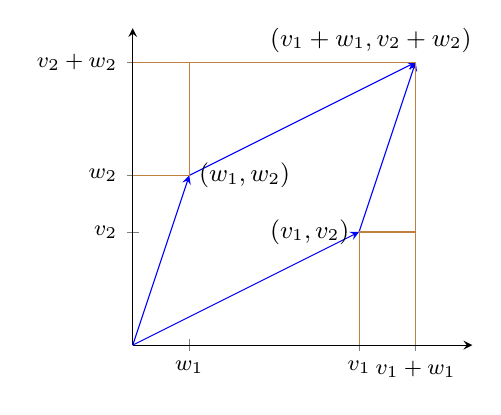
\begin{tikzpicture} 
\def\a{2} \def\b{0.5} \def\ab{2.5}
\def\c{1} \def\d{1.5} \def\cd{2.5}
\begin{axis}[axis equal image, axis lines=middle
    ,xtick={\a,\b,\ab},xticklabels={$v_1$,$w_1$,$v_1+w_1$}
    ,ytick={\c,\d,\cd},yticklabels={$v_2$,$w_2$,$v_2+w_2$}
    ,xmax=3,ymax=2.8,small
    ]
    \addplot[quiver={u=\a,v=\c},blue,-stealth] 
    coordinates {(0,0)(\b,\d)};
    \node[left] at (axis cs:\a,\c) {\small$(v_1,v_2)$};
    \addplot[quiver={u=\b,v=\d},blue,-stealth] 
    coordinates {(0,0)(\a,\c)};
    \node[right] at (axis cs:\b,\d) {\small$(w_1,w_2)$};
    \node[above] at (axis cs:\ab,\cd) {\small$(v_1+w_1,v_2+w_2) \hspace*{3.5em}$};
    \addplot[brown] coordinates {(\ab,0)(\ab,\cd)(0,\cd)};
    \addplot[brown] coordinates {(\ab,0)(\ab,\c)(\a,\c)(\a,0)};
    \addplot[brown] coordinates {(0,\cd)(\b,\cd)(\b,\d)(0,\d)};
\end{axis}
\end{tikzpicture}
\end{wrapfigure}
Consider the parallelogram drawn in blue.
It has sides given by vectors \(\vv=(v_1,v_2)\) and \(\wv=(w_1,w_2)\) as shown.
Let's determine the \idx{area} of the parallelogram. 
Its area is the containing rectangle less the two small rectangles and the four small triangles.
The two small rectangles have the same area, namely~\(w_1v_2\).
The two small triangles on the left and the right also have the same area, namely~\(\frac12w_1w_2\).
The two small triangles on the top and the bottom similarly have the same area, namely~\(\frac12v_1v_2\).
Thus, the parallelogram has 
\begin{eqnarray*}
\text{area}&=&(v_1+w_1)(v_2+w_2)-2w_1v_2-2\cdot\frac12w_1w_2-2\cdot\frac12v_1v_2
\nonumber
\\&=&v_1v_2+v_1w_2+w_1v_2+w_1w_2-2w_1v_2-w_1w_2-v_1v_2
\nonumber
\\&=&v_1w_2-v_2w_1\,. %\label{eq:cppara}
\end{eqnarray*}
In application, sometimes this right-hand side expression is negative because vectors~\vv\ and~\wv\ are the `wrong way' around.
Thus in general the \idx{parallelogram area}\({}=|v_1w_2-v_2w_1|\).


\begin{wrapfigure}[6]r{0pt}
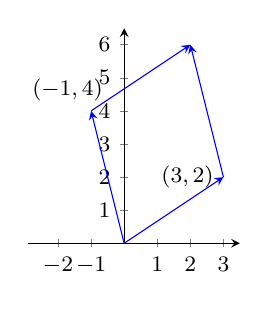
\begin{tikzpicture} 
\def\a{3} \def\b{-1} 
\def\c{2} \def\d{4} 
\begin{axis}[footnotesize,font=\footnotesize,axis equal image, axis lines=middle
    ,xmin=-2.9,xmax=3.5,ymax=6.5
    ]
    \addplot[quiver={u=\a,v=\c},blue,-stealth] 
    coordinates {(0,0)(\b,\d)};
    \node[left] at (axis cs:\a,\c) {$(\a,\c)$};
    \addplot[quiver={u=\b,v=\d},blue,-stealth] 
    coordinates {(0,0)(\a,\c)};
    \node[above] at (axis cs:\b,\d) {$(\b,\d)\qquad$};
\end{axis}
\end{tikzpicture}\end{wrapfigure}
\begin{example} 
What is the \idx{area} of the parallelogram (illustrated to the right) whose edges are formed by the vectors~\((3,2)\) and~\((-1,4)\)?
\begin{solution} 
The parallelogram area\({}=|3\cdot4-2\cdot(-1)|=|12+2|=14\)\,.  
The illustration indicates that this area must be about right as with imagination one could cut the area and move the parts about to form a rectangle roughly~\(3\) by~\(5\), and hence the area should be roughly~\(15\).
\end{solution}
\end{example}


\begingroup
\def\temp{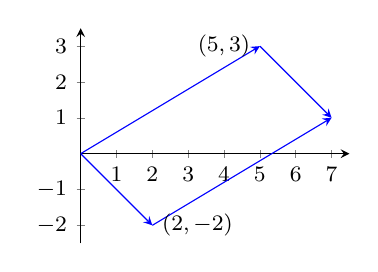
\begin{tikzpicture} 
\def\a{5} \def\b{2} \def\ab{7}
\def\c{3} \def\d{-2} \def\cd{1}
\begin{axis}[footnotesize,font=\footnotesize
    ,axis equal image, axis lines=middle
    ,ymin=-2.5,ymax=3.5,xmax=7.5
    ]
    \addplot[quiver={u=\a,v=\c},blue,-stealth] 
    coordinates {(0,0)(\b,\d)};
    \node[left] at (axis cs:\a,\c) {$(\a,\c)$};
    \addplot[quiver={u=\b,v=\d},blue,-stealth] 
    coordinates {(0,0)(\a,\c)};
    \node[right] at (axis cs:\b,\d) {$(\b,\d)$};
\end{axis}
\end{tikzpicture}}
\begin{activity}[\temp] 
What is the \idx{area} of the parallelogram (illustrated to the right) whose edges are formed by the vectors~\((5,3)\) and~\((2,-2)\)?
\actposs[4]{\(16\)}{\(4\)}{\(11\)}{\(19\)}
\vspace{1ex}
\end{activity}
\endgroup

Interestingly, we meet this expression for \idx{area}, \(v_1w_2-v_2w_1\), in another context: that of equations for a plane and its \text{normal vector.}

\index{parallelogram area|)}





\subsubsection{Normal vector to a plane}
Recall \cref{sec:nvep} introduced that we describe planes either via an equation such as \(x-y+3z=6\) or via a parametric description such as \(\xv=(1,1,2)+(1,1,0)s+(0,3,1)t\)\,.
These determine the same plane, they are just different algebraic descriptions.
One converts between these two descriptions using the \text{cross product.}




\begin{example} \label{eg:nviax}
Derive that the plane described parametrically by \(\xv=(1,1,2)+(1,1,0)s+(0,3,1)t\) has normal equation \(x-y+3z=6\)\,.
\begin{solution} 
They key to deriving the normal equation is to find that a \idx{normal vector} to the plane is~\((1,-1,3)\).
This normal vector comes from the two vectors that multiply the parameters in the parametric form, \((1,1,0)\) and~\((0,3,1)\).
The following mysterious looking procedure may be a convenient way for you to remember an otherwise involved formula: if you prefer to remember the formula of \cref{def:cp} then use that instead.
(Those who have computed \(3\times3\) determinants may recognize that the following has the same pattern---see \cref{ch:ddm}.)
Write the vectors as two consecutive columns, following a first column of the \emph{symbols} of the \idx{standard unit vector}s~\iv, \jv\ and~\kv, in
\setlength{\unitlength}{1.2ex}
\def\abc#1{\begin{vmatrix}\begin{picture}(5.3,6)
%\put(0,0){\framebox(5,5){}}
\put(0,4){$\iv$}\put(2,4){$1$}\put(4,4){$0$}
\put(0,2){$\jv$}\put(2,2){$1$}\put(4,2){$3$}
\put(0,0){$\kv$}\put(2,0){$0$}\put(4,0){$1$}
\ifnum1=#1\put(0.5,-0.5){\line(0,1)6}\put(-0.5,4.5){\line(1,0)6}\fi
\ifnum2=#1\put(0.5,-0.5){\line(0,1)6}\put(-0.5,2.5){\line(1,0)6}\fi
\ifnum3=#1\put(0.5,-0.5){\line(0,1)6}\put(-0.5,0.5){\line(1,0)6}\fi
\end{picture}\end{vmatrix}}
\def\ab#1#2#3#4{\begin{vmatrix}\begin{picture}(3,4)
\put(0,2){$#1$}\put(2,2){$#2$}
\put(0,0){$#3$}\put(2,0){$#4$}
\color{red}\put(-0.5,-0.5){\line(1,1)4}
\color{blue}\put(-0.5,3.5){\line(1,-1)4}
\end{picture}\end{vmatrix}}
\begin{eqnarray*}
\nv&=& \abc0 
\\&&\parbox{23em}{(cross out 1st column and each row in turn, multiplying each by common entry, with alternating sign)}
\\&=&\iv\abc1-\jv\abc2+\kv\abc3
\\&=&\iv\begin{vmatrix} 1&3\\0&1 \end{vmatrix}
-\jv\begin{vmatrix} 1&0\\0&1 \end{vmatrix}
+\kv\begin{vmatrix} 1&0\\1&3 \end{vmatrix}
\\&&\parbox{20em}{(draw diagonals, then subtract product of red diagonal from product of the blue)}
\\&=&\iv\ab1301
-\jv\ab1001
+\kv\ab1013
\\&=&\iv(1\cdot1-0\cdot3)
-\jv(1\cdot1-0\cdot0)
+\kv(1\cdot3-1\cdot0)
\\&=&\iv-\jv+3\kv\,.
\end{eqnarray*}
Using this normal vector, the equation of the plane must be of the form \(x-y+3z={}\)constant.
Since the plane goes through point~\((1,1,2)\), the constant\({}=1-1+3\cdot2=6\); that is, the plane is \(x-y+3z=6\) (as given).
\end{solution}
\end{example}




\begin{activity}  
Use the procedure of \cref{eg:nviax} to derive a \idx{normal vector} to the plane described in parametric form as \(\xv=(4,-1,-2)+(1,-2,1)s+(2,-3,-2)t\).  
Which of the following is your computed normal vector?
%pqr=0+round(randn(3)*2),n=cross(pqr(2,:),pqr(3,:))
\actposs[4]{\((7,4,1)\)}{\((5,6,7)\)}{\((-4,4,-10)\)}{\((2,-2,5)\)}
\end{activity}




\subsubsection{Definition of a cross product}

\paragraph{General formula}
The procedure used in \cref{eg:nviax} to derive a \idx{normal vector} leads to an algebraic formula.  
Let's apply the same procedure to two general vectors \(\vv=(v_1,v_2,v_3)\) and \(\wv=(w_1,w_2,w_3)\).
The procedure computes
{%%%%%%%%%%%%%%%%%%
\setlength{\unitlength}{1.3ex}
\def\abc#1{\begin{vmatrix}\begin{picture}(6.3,6)
%\put(0,0){\framebox(5,5){}}
\put(0,4){$\iv$}\put(2,4){$v_1$}\put(4,4){$w_1$}
\put(0,2){$\jv$}\put(2,2){$v_2$}\put(4,2){$w_2$}
\put(0,0){$\kv$}\put(2,0){$v_3$}\put(4,0){$w_3$}
\ifnum1=#1\put(0.5,-0.5){\line(0,1)6}\put(-0.5,4.5){\line(1,0)6}\fi
\ifnum2=#1\put(0.5,-0.5){\line(0,1)6}\put(-0.5,2.5){\line(1,0)6}\fi
\ifnum3=#1\put(0.5,-0.5){\line(0,1)6}\put(-0.5,0.5){\line(1,0)6}\fi
\end{picture}\end{vmatrix}}
\def\ab#1#2{\begin{vmatrix}\begin{picture}(4,4)
\put(0,2){$v_#1$}\put(2,2){$w_#1$}
\put(0,0){$v_#2$}\put(2,0){$w_#2$}
\color{red}\put(-0.5,-0.5){\line(1,1)4}
\color{blue}\put(-0.5,3.5){\line(1,-1)4}
\end{picture}\end{vmatrix}}
\begin{eqnarray*}
\nv&=& \abc0 
\\&&\parbox{23em}{(cross out 1st column and each row in turn, multiplying each by common entry, with alternating sign)}
\\&=&\iv\abc1-\jv\abc2+\kv\abc3
\\&=&\iv\begin{vmatrix} v_2&w_2\\v_3&w_3 \end{vmatrix}
-\jv\begin{vmatrix} v_1&w_1\\v_3&w_3 \end{vmatrix}
+\kv\begin{vmatrix} v_1&w_1\\v_2&w_2 \end{vmatrix}
\\&&\parbox{20em}{(draw diagonals, then subtract product of red diagonal from product of the blue)}
\\&=&\iv\ab23
-\jv\ab13
+\kv\ab12
\\&=&\iv(v_2w_3-v_3w_2)
-\jv(v_1w_3-v_3w_1)
+\kv(v_1w_2-v_2w_1).
\end{eqnarray*}
}%%%%%%%%%%%%%%%%%%%%
We use this formula to define the cross product algebraically, and then see what it means geometrically.

\begin{definition} \label{def:cp}
Let \(\vv=(v_1,v_2,v_3)\) and \(\wv=(w_1,w_2,w_3)\) be two vectors in~\(\RR^3\).
The \bfidx{cross product}  (or \bfidx{vector product}) \(\vv\times\wv\) is defined algebraically as
\index{i@$\iv$}\index{j@$\jv$}\index{k@$\kv$}%
\begin{equation*}
\vv\times\wv:=\iv(v_2w_3-v_3w_2)
+\jv(v_3w_1-v_1w_3)
+\kv(v_1w_2-v_2w_1).
\end{equation*}
\end{definition}



\begin{example} \label{eg:cpijk}
Among the \idx{standard unit vector}s, derive that 
\index{i@$\iv$}\index{j@$\jv$}\index{k@$\kv$}%
\begin{Parts}
\item \(\iv\times\jv=\kv\)\,, \item \(\jv\times\iv=-\kv\)\,,
\item \(\jv\times\kv=\iv\)\,, \item \(\kv\times\jv=-\iv\)\,,
\item \(\kv\times\iv=\jv\)\,, \item \(\iv\times\kv=-\jv\)\,,
\item \(\iv\times\iv=\jv\times\jv=\kv\times\kv=\ov\)\,.
\end{Parts}
\begin{solution} Using \cref{def:cp}:
\begin{eqnarray*}
\iv\times\jv&=&(1,0,0)\times(0,1,0)
\\&=&\iv(0\cdot0-0\cdot1)
+\jv(0\cdot0-1\cdot0)
+\kv(1\cdot1-0\cdot0)
\\&=&\kv\,;
\\\jv\times\iv&=&(0,1,0)\times(1,0,0)
\\&=&\iv(1\cdot0-0\cdot0)
+\jv(0\cdot1-0\cdot0)
+\kv(0\cdot0-1\cdot1)
\\&=&-\kv\,;
\\\iv\times\iv&=&(1,0,0)\times(1,0,0)
\\&=&\iv(0\cdot0-0\cdot0)
+\jv(0\cdot1-1\cdot0)
+\kv(1\cdot0-0\cdot1)
\\&=&\ov\,.
\end{eqnarray*}
\cref{ex:cpijk} asks you to correspondingly establish the other six identities.
\end{solution}
The cross products of this \cref{eg:cpijk} most clearly demonstrate the orthogonality of a cross product to its two argument vectors (\cref{thm:cpga}), and that the direction is in the so-called \idx{right-hand sense} (\cref{thm:cpgb}).
\end{example}




\begin{activity} 
Use \cref{def:cp} to find the cross product of \((-4,1,-1)\) and \((-2,2,1)\) is which one of the following:
\actposs[4]{\((3,6,-6)\)}{\((-3,-6,6)\)}{\((3,-6,-6)\)}{\((-3,-6,6)\)}
\end{activity}



\needlines9
\subsubsection{Geometry of a cross product}


\begin{example}[\idx{parallelogram area}] \label{eg:cppara}
Let's revisit the introduction to this section.
Consider the parallelogram in the \(x_1x_2\)-plane with edges formed by the \(\RR^3\)~vectors \(\vv=(v_1,v_2,0)\) and \(\wv=(w_1,w_2,0)\).
At the start of this \cref{sec:cp} we derived that the parallelogram formed by these vectors has \idx{area}\({}=|v_1w_2-v_2w_1|\).
Compare this area with the cross product
\begin{eqnarray*}
\vv\times\wv&=&\iv(v_2\cdot0-0\cdot w_2)
+\jv(0\cdot w_1-v_1\cdot0)
+\kv(v_1w_2-v_2w_1)
\\&=&\iv0+\jv0+\kv(v_1w_2-v_2w_1)
\\&=&\kv(v_1w_2-v_2w_1).
\end{eqnarray*}
Consequently, the \idx{length} of this cross product equals the area of the parallelogram formed by~\vv\ and~\wv\ (\cref{thm:cpgd}).
(Also the direction of the cross product,~\(\pm\kv\), is orthogonal to the \(x_1x_2\)-plane containing the two vectors---\cref{thm:cpga}).
\end{example}


\begingroup
\def\temp{\qview{30}{35}{\begin{tikzpicture} 
\begin{axis}[footnotesize,font=\footnotesize,axis equal,view={\q}{30}
    ,xlabel={$x_1$},ylabel={$x_2$},zlabel={$x_3$},label shift={-1.5ex}
    ]
    \threev[above]20{0.5}{\vec v};
    \threev[above]102{\vec w};
\end{axis}
\end{tikzpicture}}}
\begin{activity}[\temp]
Using property \ref{thm:cpgb} of the next theorem, in which direction is the cross product \(\vv\times\wv\) for the two vectors illustrated in stereo to the right?
\actposs{\(-\jv\)}{\(+\iv\)}{\(+\jv\)}{\(-\iv\)}
\end{activity}
\endgroup



\begin{figbox}{\begin{tikzpicture}
  \begin{axis}[small,thick, axis lines=none,ymax=1.3,ymin=-0.3,xmin=-0.3,xmax=1.3]
    \addplot graphics [xmin=0,xmax=1,ymin=0,ymax=1]
      {Vectors/right-hand-rule.jpg};
      % this is AJRs photo of AJRs hand
    \addplot[blue,quiver={u=-0.05,v=0.5,scale arrows=1.07},-stealth] coordinates {(0.55,0.55)};
    \node[above] at (axis cs:0.5,1.05) {$\vv$};
    \addplot[blue,quiver={u=-0.6,v=0.2,scale arrows=1.07},-stealth] coordinates {(0.55,0.55)};
    \node[left] at (axis cs:-0.05,0.77) {$\wv$};
    \addplot[blue,quiver={u=-0.4,v=-0.6,scale arrows=1.07},-stealth] coordinates {(0.55,0.55)};
    \node[below] at (axis cs:0.15,-0.05) {$\vv\times\wv$};
  \end{axis}
\end{tikzpicture}}%
\begin{theorem}[cross product geometry] \label{thm:cpg}
Let \vv\ and~\wv\ be two vectors in~\(\RR^3\):
\begin{enumerate}[ref=\ref{thm:cpg}(\alph*)]
\item\label[theorem]{thm:cpga} the vector~\(\vv\times\wv\) is \idx{orthogonal} to both~\vv\ and~\wv;

\item\label[theorem]{thm:cpgb} 
the \index{cross product direction}direction of~\(\vv\times\wv\) is in the \bfidx{right-hand sense}%
in that if \vv~is in the direction of your thumb, and \wv~is in the direction of your straight index finger, then \(\vv\times\wv\) is in the direction of your bent second\slash longest finger---all on your right-hand as illustrated to \text{the right;} 

\item\label[theorem]{thm:cpgc} \(|\vv\times\wv|=|\vv|\,|\wv|\sin\theta\) where \(\theta\)~is the \idx{angle} between vectors~\vv\ and~\wv\ (\(0\leq\theta\leq\pi\), equivalently \(0^\circ\leq\theta\leq180^\circ\)); and

\item\label[theorem]{thm:cpgd} the \idx{length}~\(|\vv\times\wv|\) is the \idx{area} of the parallelogram\index{parallelogram area} with edges~\vv\ and~\wv.
\end{enumerate}
\end{theorem}
\end{figbox}



\begin{proof} 
Let \(\vv=(v_1,v_2,v_3)\) and \(\wv=(w_1,w_2,w_3)\).

\begin{description}
\item[\ref{thm:cpga}] Recall that two vectors are orthogonal if their dot product is zero (\cref{def:orthovec}).
To determine orthogonality between~\vv\ and the cross product \(\vv\times\wv\), consider
\begin{eqnarray*}
\vv\cdot(\vv\times\wv)
&=&(v_1\iv+v_2\jv+v_3\kv)
\cdot\big[\iv(v_2w_3-v_3w_2)
\\&&{}
+\jv(v_3w_1-v_1w_3)
+\kv(v_1w_2-v_2w_1)\big]
\\&=&v_1(v_2w_3-v_3w_2)
+v_2(v_3w_1-v_1w_3)
\\&&{}
+v_3(v_1w_2-v_2w_1)
\\&=&v_1v_2w_3-v_1v_3w_2
+v_2v_3w_1
\\&&{}
-v_1v_2w_3
+v_1v_3w_2-v_2v_3w_1
\quad{}=0
\end{eqnarray*}
as each term in the penultimate line cancels with the term underneath in the last line.
Since the dot product is zero, the cross product \(\vv\times\wv\) is orthogonal to vector~\vv.

Similarly, \(\vv\times\wv\) is orthogonal to~\wv\  (\cref{ex:cpga}).

\item[\ref{thm:cpgb}] This right-handed property follows from the convention that the \idx{standard unit vector}s~\iv, \jv\ and~\kv\ are right-handed: that if \iv~is in the direction of your thumb, and \jv~is in the direction of your straight index finger, then \kv~is in the direction of your bent second\slash longest finger---all on your right-hand.

We prove only for the case of vectors in the \(x_1x_2\)-plane, in which case \(\vv=(v_1,v_2,0)\) and \(\wv=(w_1,w_2,0)\), and when both \(v_1,w_1>0\)\,.
One example is in stereo below.
\begin{center}
\qview{30}{35}{\begin{tikzpicture} 
\def\a{1.5} \def\b{0.5} 
\def\c{1} \def\d{2} 
\begin{axis}[footnotesize,font=\footnotesize,axis equal,view={\q}{30}
    ,xmin=-0.4,xmax=2.4,ymin=-0.4,ymax=2.4,xtick={0,1,2},ztick={0,1}
    ,xlabel={$x_1$},ylabel={$x_2$},zlabel={$x_3$},label shift={-1.5ex}
    ]
    \addplot3[quiver={u=\a,v=\c,w=0},blue,-stealth,thick] 
    coordinates {(0,0,0)};
    \node[right] at (axis cs:\a,\c,0) {$\vv$};
    \addplot3[quiver={u=\b,v=\d,w=0},blue,-stealth,thick] 
    coordinates {(0,0,0)};
    \node[above] at (axis cs:\b,\d,0) {$\wv$};
    \addplot3[quiver={u=0,v=0,w=1},red,-stealth,thick] 
    coordinates {(0,0,0)};
    \node[above] at (axis cs:0,0,1) {$+\kv$};
\end{axis}
\end{tikzpicture}}
\end{center}
\cref{eg:cppara} derived the cross product \(\vv\times\wv=\kv(v_1w_2-v_2w_1)\).
Consequently, this cross product is in the~\(+\kv\) direction only when \(v_1w_2-v_2w_1>0\) (it is in the~\(-\kv\) direction in the complementary case when \(v_1w_2-v_2w_1<0\)). 
This inequality for~\(+\kv\) rearranges to \(v_1w_2>v_2w_1\)\,.
Dividing by the positive~\(v_1w_1\) requires \(\frac{w_2}{w_1}>\frac{v_2}{v_1}\)\,.
That is, in the \(x_1x_2\)-plane the `slope' of vector~\wv\ must be greater than the `slope' of vector~\vv.
In this case, if \vv~is in the direction of your thumb on your right-hand, and \wv~is in the direction of your straight index finger, then your bent second\slash longest finger is in the direction~\(+\kv\) as required by the cross-product \(\vv\times\wv\)\,.

\item[\ref{thm:cpgc}] \cref{ex:cpgc} establishes the identity \(|\vv\times\wv|^2=|\vv|^2|\wv|^2-(\vv\cdot\wv)^2\).
From \cref{thm:anglev} substitute \(\vv\cdot\wv=|\vv||\wv|\cos\theta\) into this identity:
\begin{eqnarray*}
|\vv\times\wv|^2&=&|\vv|^2|\wv|^2-(\vv\cdot\wv)^2
\\&=&|\vv|^2|\wv|^2-(|\vv||\wv|\cos\theta)^2
\\&=&|\vv|^2|\wv|^2-|\vv|^2|\wv|^2\cos^2\theta
\\&=&|\vv|^2|\wv|^2(1-\cos^2\theta)
\\&=&|\vv|^2|\wv|^2\sin^2\theta\,.
\end{eqnarray*}
Take the square-root of both sides to determine \(|\vv\times\wv|=\pm|\vv||\wv|\sin\theta\)\,.
But \(\sin\theta\geq0\) since the angle \(0\leq\theta\leq\pi\)\,, and all the lengths are also\({}\geq0\)\,, so only the plus case applies.
That is, the length \(|\vv\times\wv|=|\vv||\wv|\sin\theta\) \text{as required.}

\item[\ref{thm:cpgd}] \ \\
\begin{figbox}{\rotatebox{20}{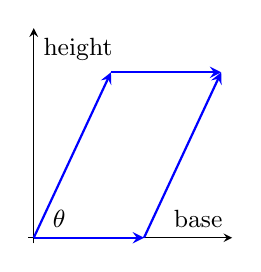
\begin{tikzpicture} 
\def\a{1} \def\b{0.7} 
\def\c{0} \def\d{1.5} 
\begin{axis}[axis equal image, axis lines=middle,xtick={0},ytick={0}
    ,xmax=1.8,ymax=1.9,ymin=-0.05,xmin=-0.05,footnotesize,font=\small
    ,xlabel={base},ylabel={height}
    ]
    \addplot[quiver={u=\a,v=\c},blue,-stealth,thick] 
    coordinates {(0,0)(\b,\d)};
    \node[above] at (axis cs:\a,\c) {$\vv\quad$};
    \addplot[quiver={u=\b,v=\d},blue,-stealth,thick] 
    coordinates {(0,0)(\a,\c)};
    \node[left] at (axis cs:\b,\d) {$\wv$};
    \node[above] at (axis cs:0,0) {$\qquad\theta$};
\end{axis}
\end{tikzpicture}}}
Consider the plane containing the vectors~\vv\ and~\wv, 
and hence containing the parallelogram formed by these vectors---as illustrated to the right.
Using vector~\vv\ as the base of the parallelogram, with length~\(|\vv|\), by basic trigonometry the height of the parallelogram is then \(|\wv|\sin\theta\).
Hence the area of the parallelogram is the product 
\(\text{base}\cdot\text{height}=|\vv||\wv|\sin\theta=|\vv\times\wv|\) by the previous part~\ref{thm:cpgc}.\end{figbox}
\end{description}
\end{proof}

\begin{wrapfigure}[7]r{0pt}
\qview{30}{34}{\begin{tikzpicture} 
\def\a{-2} \def\b{2} 
\def\c{0} \def\d{2} 
\def\e{1} \def\f{1}
\begin{axis}[footnotesize,font=\footnotesize,axis equal,view={\q}{25}
    ,xlabel={$x_1$},ylabel={$x_2$},zlabel={$x_3$},label shift={-1.5ex}
    ,ytick={0,2} ]
    \threev[above]{\a}{\c}{\e}{\vec v};
    \addplot3[quiver={u=\a,v=\c,w=\e},blue,-stealth,thick] 
    coordinates {(\b,\d,\f)};
    \threev[above]{\b}{\d}{\f}{\vec w};
    \addplot3[quiver={u=\b,v=\d,w=\f},blue,-stealth,thick] 
    coordinates {(\a,\c,\e)};
    \addplot3[gray] coordinates 
    {((\a)+(\b),(\c)+(\d),0)((\a)+(\b),(\c)+(\d),\e+\f)};
\end{axis}
\end{tikzpicture}}
\end{wrapfigure}
\begin{example} \label{eg:apvw}
Find the \idx{area} of the parallelogram\index{parallelogram area} with edges formed by vectors
\(\vv=(-2,0,1)\) and \(\wv=(2,2,1)\)---as illustrated in stereo.
\begin{solution} 
The area is the length of the cross product
\begin{eqnarray*}
\vv\times\wv
&=&\iv(0\cdot 1-1\cdot 2)
+\jv(1\cdot 2-(-2)\cdot 1)
+\kv((-2)\cdot 2-0\cdot 2)
\\&=&-2\iv+4\jv-4\kv\,.
\end{eqnarray*}
Then the parallelogram area \(|\vv\times\wv|=\sqrt{(-2)^2+4^2+(-4)^2}
=\sqrt{4+16+16}=\sqrt{36}=6\)\,.
\aqed\par
\end{solution}
\end{example}

\begingroup
\def\temp{\qview{30}{34}{\begin{tikzpicture} 
\def\a{-2} \def\b{2} 
\def\c{-1} \def\d{0} 
\def\e{0} \def\f{-1}
\begin{axis}[footnotesize,font=\footnotesize,axis equal,view={\q}{25}
    ,xlabel={$x_1$},ylabel={$x_2$},zlabel={$x_3$},label shift={-1.5ex}
    ,ytick={-2,0} ]
    \threev[above]{\a}{\c}{\e}{\vec v};
    \addplot3[quiver={u=\a,v=\c,w=\e},blue,-stealth,thick] 
    coordinates {(\b,\d,\f)};
    \threev[above]{\b}{\d}{\f}{\vec w};
    \addplot3[quiver={u=\b,v=\d,w=\f},blue,-stealth,thick] 
    coordinates {(\a,\c,\e)};
    \addplot3[gray] coordinates 
    {((\a)+(\b),(\c)+(\d),0)((\a)+(\b),(\c)+(\d),\e+\f)};
\end{axis}
\end{tikzpicture}}}
\begin{activity}[\temp]
% u=0+round(randn(1,3)*3), v=0+round(randn(1,3)*3), uv=cross(u,v), area=norm(uv)
What is the \idx{area} of the parallelogram\index{parallelogram area} (in stereo to the right) with edges formed by vectors
\(\vv=(-2,1,0)\) and \(\wv=(2,0,-1)\)?
\actposs{\(3\)}{\(1\)}{\(\sqrt{5}\)}{\(5\)}
\end{activity}
\endgroup





\begin{wrapfigure}r{0pt}
\qview{26}{31}{\begin{tikzpicture} 
\def\a{-2} \def\b{2} 
\def\c{3} \def\d{2} 
\def\e{2} \def\f{3}
\begin{axis}[footnotesize,font=\footnotesize,axis equal,view={\q}{25}
    ,xlabel={$x_1$},ylabel={$x_2$},zlabel={$x_3$},label shift={-1.5ex}
    ]
    \threev[above]{\a}{\c}{\e}{\vec v};
    \threev[above]{\b}{\d}{\f}{\vec w};
    \addplot3[quiver={u=1,v=2,w=-2},red,-stealth,thick] 
    coordinates {(0,0,0)};
    \node[below] at (axis cs:1,2,-2) {$\nv$};
\end{axis}
\end{tikzpicture}}
\end{wrapfigure}
\begin{example} \label{eg:cpnvp}
Find a \idx{normal vector} to the plane containing the two vectors \(\vv=-2\iv+3\jv+2\kv\) and \(\wv=2\iv+2\jv+3\kv\) ---illustrated below.
Hence find an \idx{equation of the plane} given parametrically as \(\xv=-2\iv-\jv+3\kv+(-2\iv+3\jv+2\kv)s+(2\iv+2\jv+3\kv)t\)\,.
\index{i@$\iv$}\index{j@$\jv$}\index{k@$\kv$}%

\begin{solution} 
Use \cref{def:cp} of the cross-product to find a normal vector:
\begin{eqnarray*}
\vv\times\wv&=&
\iv(3\cdot 3-2\cdot 2)
+\jv(2\cdot 2-(-2)\cdot 3)
+\kv((-2)\cdot 2-3\cdot 2)
\\&=&5\iv+10\jv-10\kv\,.
\end{eqnarray*}
A normal vector is any vector proportional to this, so we could divide by five and choose normal vector \(\nv=\iv+2\jv-2\kv\) (as illustrated above).

An equation of the plane through \(-2\iv-\jv+3\kv\) is then given by the dot product
\begin{eqnarray*}
&&(\iv+2\jv-2\kv)\cdot[(x+2)\iv+(y+1)\jv+(z-3)\kv]=0\,,
\\\text{that is,}&& x+2+2y+2-2z+6=0\,,
\\\text{that is,}&& x+2y-2z+10=0
\end{eqnarray*}
is the required normal equation of the plane.
\aqed
\end{solution}
\end{example}




\subsubsection{Algebraic properties of a cross product}

\cref{ex:cppa,ex:cppb,ex:cppc} establish three of the following four useful algebraic properties of the cross product.

\begin{theorem}[cross product properties] \label{thm:cpp}
Let \uv, \vv\ and~\wv\ be vectors in~\(\RR^3\), and \(c\)~be a \idx{scalar}:
\begin{enumerate}[ref=\ref{thm:cpp}(\alph*)]
\item\label[theorem]{thm:cppz} \(\vv\times\vv=\ov\);
\item\label[theorem]{thm:cppa} \(\wv\times\vv=-(\vv\times\wv)\) \quad(not commutative);\index{commutative law}
\item\label[theorem]{thm:cppb} \((c\vv)\times\wv=c(\vv\times\wv)=\vv\times(c\wv)\);
\item\label[theorem]{thm:cppc} \(\uv\times(\vv+\wv)=\uv\times\vv+\uv\times\wv\) \quad(\idx{distributive law}).
\end{enumerate}
\end{theorem}


\begin{proof} 
Let's prove property~\ref{thm:cppz} two ways---algebraically and geometrically.  \cref{ex:cppa,ex:cppb,ex:cppc} ask you to prove the other properties.
\begin{itemize}
\item Algebraically:  with vector \(\vv=(v_1,v_2,v_3)\),  \cref{def:cp} gives
\begin{eqnarray*}
\vv\times\vv
&=&\iv(v_2v_3-v_3v_2)
+\jv(v_3v_1-v_1v_3)
+\kv(v_1v_2-v_2v_1)
\\&=&0\iv+0\jv+0\kv=\ov\,.
\end{eqnarray*}
\item Geometrically: 
%from \cref{thm:cpgc} \(|\vv\times\vv|=|\vv||\vv|\sin\theta\) where \(\theta\)~is the angle between~\vv\ and~\vv, and so \(\theta=0\)\,.
%Since \(\sin\theta=\sin0=0\)\,, the length \(|\vv\times\vv|=0\) and so \(\vv\time\vv=\ov\) (\cref{thm:veclen0}).
from \cref{thm:cpgd}, \(|\vv\times\vv|\) is the area of the parallelogram with edges~\vv\ and~\vv.
But such a parallelogram has zero area, so \(|\vv\times\vv|=0\)\,.
Since the only vector of length zero is the zero vector (\cref{thm:veclen0}), \(\vv\times\vv=\ov\).
\end{itemize}
\end{proof}





\begin{example} 
As an example of \cref{thm:cppa}, \cref{eg:cpijk} shows that \(\iv\times\jv=\kv\)\,, whereas reversing the order of the cross product gives the negative \(\jv\times\iv=-\kv\)\,.  
Given \cref{eg:cpnvp} derived \(\vv\times\wv=5\iv+10\jv-10\kv\) in the case when \(\vv=-2\iv+3\jv+2\kv\) and \(\wv=2\iv+2\jv+3\kv\)\,, what is \(\wv\times\vv\)?
\begin{solution} 
By \ref{thm:cppa},
\(\wv\times\vv=-(\vv\times\wv)=-5\iv-10\jv+10\kv\)\,.
\end{solution}
\end{example}


\begin{example} 
Given \((\iv+\jv+\kv)\times(-2\iv-\jv)=\iv-2\jv+\kv\)\,, what is \((3\iv+3\jv+3\kv)\times(-2\iv-\jv)\)?
\begin{solution} 
The first vector is \(3(\iv+\jv+\kv)\) so by \cref{thm:cppb},
\begin{align*}
&(3\iv+3\jv+3\kv)\times(-2\iv-\jv)
\\&=[3(\iv+\jv+\kv)]\times(-2\iv-\jv)
\\&=3[(\iv+\jv+\kv)\times(-2\iv-\jv)]
\\&=3[\iv-2\jv+\kv]=3\iv-6\jv+3\kv\,.
\end{align*}
\end{solution}
\end{example}


\begin{activity}  
For vectors \(\uv=-\iv+3\kv\)\,, \(\vv=\iv+3\jv+5\kv\)\,, and \(\wv=-2\iv+\jv-\kv\) you are given that 
\begin{eqnarray*}
&&\uv\times\vv=-9\iv+8\jv-3\kv\,,
\\&&\uv\times\wv=-3\iv-7\jv-\kv\,,
\\&&\vv\times\wv=-8\iv-9\jv+7\kv\,.
\end{eqnarray*}
Which is the cross product \((-\iv+3\kv)\times(-\iv+4\jv+4\kv)\)?
\actposs{\(-12\iv+\jv-4\kv\)}
{\(\iv-17\jv+10\kv\)}
{\(-11\iv-16\jv+6\kv\)}
{\(-17\iv-\jv+4\kv\)}
Also, which is \((\iv+3\jv+5\kv)\times(-3\iv+\jv+2\kv)\)? %\(\iv-17\jv+10\kv\)
\end{activity}



\begin{reduce}
\begin{example} 
The properties of \cref{thm:cpp} empower algebraic manipulation.
Use such algebraic manipulation, and the identities among \idx{standard unit vector}s of \cref{eg:cpijk}, compute the cross product \((\iv-\jv)\times(4\iv+2\kv)\).
\begin{solution} In full detail:
\begin{align*}
&(\iv-\jv)\times(4\iv+2\kv)
\\&=(\iv-\jv)\times(4\iv)+(\iv-\jv)\times(2\kv) 
\quad(\text{by \ref{thm:cppc}})
\\&=4(\iv-\jv)\times\iv+2(\iv-\jv)\times\kv
\quad(\text{by \ref{thm:cppb}})
\\&=-4\iv\times(\iv-\jv)-2\kv\times(\iv-\jv)
\quad(\text{by \ref{thm:cppa}})
\\&=-4[\iv\times\iv+\iv\times(-\jv)]-2[\kv\times\iv+\kv\times(-\jv)]
\quad(\text{by \ref{thm:cppc}})
\\&=-4[\iv\times\iv-\iv\times\jv]-2[\kv\times\iv-\kv\times\jv]
\quad(\text{by \ref{thm:cppb}})
\\&=-4[\ov-\kv]-2[\jv-(-\iv)]
\quad(\text{by \cref{eg:cpijk}})
\\&=-2\iv-2\jv+4\kv\,.
\end{align*}
\end{solution}
\end{example}
\end{reduce}







\subsubsection{Volume of a parallelepiped}

\index{parallelepiped volume|(}
\newcommand{\pppd}[1]{% draw a parallelepiped
\qview{30}{34}{\begin{tikzpicture} 
\def\ua{0.5}\def\ub{0.5}\def\uc{1}
\def\va{2}\def\vb{0.5}\def\vc{0}
\def\wa{0.5}\def\wb{1.3}\def\wc{0}
\def\vw{1.7}
\begin{axis}[small,font=\footnotesize,axis equal,view={\q}{25}
    ,axis lines=none ]
    \addplot3[quiver={u=\ua,v=\ub,w=\uc},blue,-stealth,thick] 
    coordinates {(0,0,0)(\va,\vb,\vc)(\wa,\wb,\wc)(\va+\wa,\vb+\wb,\vc+\wc)};
    \node[below] at (axis cs:\ua,\ub,\uc) {$\vec u$};
    \addplot3[quiver={u=\va,v=\vb,w=\vc},blue,-stealth,thick] 
    coordinates {(0,0,0)(\ua,\ub,\uc)(\wa,\wb,\wc)(\ua+\wa,\ub+\wb,\uc+\wc)};
    \node[below] at (axis cs:\va,\vb,\vc) {$\vec v$};
    \addplot3[quiver={u=\wa,v=\wb,w=\wc},blue,-stealth,thick] 
    coordinates {(0,0,0)(\va,\vb,\vc)(\ua,\ub,\uc)(\va+\ua,\vb+\ub,\vc+\uc)};
    \node[below] at (axis cs:\wa,\wb,\wc) {$\vec w$};
  \ifnum0<#1
    \addplot3[quiver={u=0,v=0,w=\vw},red,-stealth,thick] 
    coordinates {(0,0,0)};
    \node[right] at (axis cs:0,0,\vw) {$\vec v\times\vec w$};
    \node[right] at (axis cs:0,0,0.5) {$\!\theta$};
    \addplot3[gray] coordinates {(0,0,\uc)(\ua,\ub,\uc)};
  \fi
\end{axis}
\end{tikzpicture}
}}


\begin{wrapfigure}r{0pt} \pppd0\end{wrapfigure}
Consider the \idx{parallelepiped} with edges formed by three vectors~\uv, \vv\ and~\wv\ in~\(\RR^3\), as illustrated in stereo to the right.
Our challenge is to derive that the volume of the parallelepiped is~\(|\uv\cdot(\vv\times\wv)|\).

\index{volume, parallelepiped}%
Let's use that we know the volume of the parallelepiped is the area of its base times its height.
\begin{itemize}
\item The base of the parallelepiped is the \idx{parallelogram} formed with edges~\vv\ and~\wv.
Hence the base has area~\(|\vv\times\wv|\) (\cref{thm:cpgd}).

\item 
\begin{figbox}{\pppd1}
The height of the parallelepiped is then that part of~\uv\ in the direction of a \idx{normal vector} to~\vv\ and~\wv.
We know that \(\vv\times\wv\) is orthogonal to both~\vv\ and~\wv\ (\cref{thm:cpga}), so by trigonometry the height must be \(|\uv|\cos\theta\) for angle~\(\theta\) between~\uv\ and \(\vv\times\wv\), as illustrated.
\end{figbox}

To cater for cases where \(\vv\times\wv\) points in the opposite direction to that shown, the height is~\(|\uv||\cos\theta|\).
The \idx{dot product}  determines this \idx{cosine} (\cref{thm:anglev}):
\begin{equation*}
\cos\theta=\frac{\uv\cdot(\vv\times\wv)}{|\uv||\vv\times\wv|}\,.
\end{equation*}
The height of the parallelepiped is then
\begin{equation*}
|\uv||\cos\theta|=|\uv|\frac{|\uv\cdot(\vv\times\wv)|}{|\uv||\vv\times\wv|}
=\frac{|\uv\cdot(\vv\times\wv)|}{|\vv\times\wv|}\,.
\end{equation*}
\end{itemize}
Consequently, the volume of the parallelepiped equals
\begin{equation*}
\text{base}\cdot\text{height}
=|\vv\times\wv|\frac{|\uv\cdot(\vv\times\wv)|}{|\vv\times\wv|}
=|\uv\cdot(\vv\times\wv)|.
\end{equation*}



\begin{definition} \label{def:sctrpr}
For every three vectors \uv, \vv\ and~\wv\ in~\(\RR^3\), the \bfidx{scalar triple product}\index{triple product, scalar} is \(\uv\cdot(\vv\times\wv)\).
\end{definition}



\begin{wrapfigure}r{0pt}
\qview{30}{34}{\begin{tikzpicture} 
\def\ua{0}\def\ub{2}\def\uc{1}
\def\va{-2}\def\vb{0}\def\vc{1}
\def\wa{2}\def\wb{2}\def\wc{1}
\begin{axis}[footnotesize,font=\footnotesize,axis equal,view={\q}{25}
    ,xlabel={$x_1$},ylabel={$x_2$},zlabel={$x_3$},label shift={-1.5ex} 
    ]
    \addplot3[quiver={u=\ua,v=\ub,w=\uc},blue,-stealth,thick] 
    coordinates {(0,0,0)(\va,\vb,\vc)(\wa,\wb,\wc)(\va+\wa,\vb+\wb,\vc+\wc)};
    \node[below] at (axis cs:\ua,\ub,\uc) {$\vec u$};
    \addplot3[quiver={u=\va,v=\vb,w=\vc},blue,-stealth,thick] 
    coordinates {(0,0,0)(\ua,\ub,\uc)(\wa,\wb,\wc)(\ua+\wa,\ub+\wb,\uc+\wc)};
    \node[left] at (axis cs:\va,\vb,\vc) {$\vec v$};
    \addplot3[quiver={u=\wa,v=\wb,w=\wc},blue,-stealth,thick] 
    coordinates {(0,0,0)(\va,\vb,\vc)(\ua,\ub,\uc)(\va+\ua,\vb+\ub,\uc+\vc)};
    \node[below] at (axis cs:\wa,\wb,\wc) {$\vec w$};
\end{axis}
\end{tikzpicture}}
\end{wrapfigure}
\begin{example} \label{eg:stppv}
Use the \idx{scalar triple product} to find the volume of the parallelepiped formed by vectors \(\uv=(0,2,1)\), \(\vv=(-2,0,1)\) and \(\wv=(2,2,1)\)---as illustrated in stereo to the right.

\begin{solution} 
\cref{eg:apvw} found the cross product \(\vv\times\wv=-2\iv+4\jv-4\kv\)\,.
So the scalar triple product \(\uv\cdot(\vv\times\wv)=(2\jv+\kv)\cdot(-2\iv+4\jv-4\kv)=8-4=4\)\,.
Hence the volume of the parallelepiped is~\(4\) (cubic units). 

The order of the vectors in a scalar triple product only affects the sign of the result.  
For example, we also find the volume of this parallelepiped via~\(\vv\cdot(\uv\times\wv)\).
Returning to the procedure of \cref{eg:nviax} to find the cross product gives
\setlength{\unitlength}{1.2ex}
\def\abc#1{\begin{vmatrix}\begin{picture}(5.3,6)
%\put(0,0){\framebox(5,5){}}
\put(0,4){$\iv$}\put(2,4){$0$}\put(4,4){$2$}
\put(0,2){$\jv$}\put(2,2){$2$}\put(4,2){$2$}
\put(0,0){$\kv$}\put(2,0){$1$}\put(4,0){$1$}
\ifnum1=#1\put(0.5,-0.5){\line(0,1)6}\put(-0.5,4.5){\line(1,0)6}\fi
\ifnum2=#1\put(0.5,-0.5){\line(0,1)6}\put(-0.5,2.5){\line(1,0)6}\fi
\ifnum3=#1\put(0.5,-0.5){\line(0,1)6}\put(-0.5,0.5){\line(1,0)6}\fi
\end{picture}\end{vmatrix}}
\def\ab#1#2#3#4{\begin{vmatrix}\begin{picture}(3,4)
\put(0,2){$#1$}\put(2,2){$#2$}
\put(0,0){$#3$}\put(2,0){$#4$}
\color{red}\put(-0.5,-0.5){\line(1,1)4}
\color{blue}\put(-0.5,3.5){\line(1,-1)4}
\end{picture}\end{vmatrix}}
\begin{eqnarray*}
\uv\times\wv&=& \abc0 
%\\&&\parbox{20em}{(cross out 1st column and each row, multiplying each by common entry, with alternating sign)}
\\&=&\iv\abc1-\jv\abc2+\kv\abc3
\\&=&\iv\begin{vmatrix} 2&2\\1&1 \end{vmatrix}
-\jv\begin{vmatrix} 0&2\\1&1 \end{vmatrix}
+\kv\begin{vmatrix} 0&2\\2&2 \end{vmatrix}
%\\&&\parbox{20em}{(draw diagonals, then subtract product of red diagonal from product of the blue)}
\\&=&\iv\ab2211
-\jv\ab0211
+\kv\ab0222
\\&=&\iv(2\cdot1-1\cdot2)
-\jv(0\cdot1-1\cdot2)
+\kv(0\cdot2-2\cdot2)
\\&=&2\jv-4\kv\,.
\end{eqnarray*}
Then the triple product \(\vv\cdot(\uv\times\wv)=(-2\iv+\kv)\cdot(2\jv-4\kv)=0+0-4=-4\)\,.
Hence the volume of the parallelepiped is~\(|-4|=4\) as before.
\end{solution}
\end{example}



Using the procedure of \cref{eg:nviax} to find a \idx{scalar triple product} establishes a strong connection to the matrix \idx{determinant}s of \cref{ch:ddm}.
\index{i@$\iv$}\index{j@$\jv$}\index{k@$\kv$}%
In the second solution to the previous \cref{eg:stppv}, in finding \(\uv\times\wv\), the unit vectors~\iv, \jv\ and~\kv\  just acted as place holding symbols to eventually ensure a multiplication by the correct component of~\vv\ in the dot product.
We could seamlessly combine the two products by replacing the symbols~\iv, \jv\ and~\kv\ directly with the corresponding component of~\vv:
{%%%%%%
\setlength{\unitlength}{1.6ex}
\def\abc#1{\begin{vmatrix}\ \begin{picture}(5.3,6)
%\put(0,0){\framebox(5,5){}}
\put(0,4){$\!\!\!-2$}\put(2,4){$0$}\put(4,4){$2$}
\put(0,2){$0$}\put(2,2){$2$}\put(4,2){$2$}
\put(0,0){$1$}\put(2,0){$1$}\put(4,0){$1$}
\ifnum1=#1\put(0.5,-0.5){\line(0,1)6}\put(-0.5,4.5){\line(1,0)6}\fi
\ifnum2=#1\put(0.5,-0.5){\line(0,1)6}\put(-0.5,2.5){\line(1,0)6}\fi
\ifnum3=#1\put(0.5,-0.5){\line(0,1)6}\put(-0.5,0.5){\line(1,0)6}\fi
\end{picture}\end{vmatrix}}
\def\ab#1#2#3#4{\begin{vmatrix}\begin{picture}(3,4)
\put(0,2){$#1$}\put(2,2){$#2$}
\put(0,0){$#3$}\put(2,0){$#4$}
\color{red}\put(-0.5,-0.5){\line(1,1)4}
\color{blue}\put(-0.5,3.5){\line(1,-1)4}
\end{picture}\end{vmatrix}}
\begin{eqnarray*}
\vv\cdot(\uv\times\wv)&=& \abc0 
%\\&&\parbox{20em}{(cross out 1st column and each row, multiplying each by common entry, with alternating sign)}
\\&=&-2\abc1-0\abc2+1\abc3
\\&=&-2\begin{vmatrix} 2&2\\1&1 \end{vmatrix}
-0\begin{vmatrix} 0&2\\1&1 \end{vmatrix}
+1\begin{vmatrix} 0&2\\2&2 \end{vmatrix}
%\\&&\parbox{20em}{(draw diagonals, then subtract product of red diagonal from product of the blue)}
\\&=&-2\ab2211
-0\ab0211
+1\ab0222
\\&=&-2(2\cdot1-1\cdot2)
-0(0\cdot1-1\cdot2)
+1(0\cdot2-2\cdot2)
\\&=&-2\cdot0-0(-2)+1(-4)=-4\,.
\end{eqnarray*}
}%%%%%%%%%%%%%%%%%%%%
Hence the parallelepiped formed by~\uv, \vv\ and~\wv\ has volume~\(|-4|\), as before.
Here the volume follows from the above manipulations of the matrix of numbers formed with columns of the matrix being the vectors~\uv, \vv\ and~\wv.
\cref{ch:ddm} shows that this computation of volume generalizes to determining, via analogous matrices of vectors, the `volume' of objects formed by vectors with any number \text{of components.}


\index{parallelepiped volume|)}


\index{cross product|)}




\sectionExercises


\begin{exercise} \label{ex:cpijk} 
Use \cref{def:cp} to establish some of the \idx{standard unit vector} identities in \cref{eg:cpijk}: 
\index{i@$\iv$}\index{j@$\jv$}\index{k@$\kv$}%
\begin{enumerate}
\item \(\jv\times\kv=\iv\)\,,\quad \(\kv\times\jv=-\iv\)\,,\quad \(\jv\times\jv=\ov\)\,;
\item \(\kv\times\iv=\jv\)\,,\quad \(\iv\times\kv=-\jv\)\,,\quad \(\kv\times\kv=\ov\)\,.
\end{enumerate}
\end{exercise}





\begin{exercise}  
Use \cref{def:cp}, perhaps via the procedure used in \cref{eg:nviax}, to determine the following cross products. 
Confirm each cross product is orthogonal to the two vectors in the given product.
Show your details.
% u=0+round(randn(1,3)*3), v=0+round(randn(1,3)*3), uv=cross(u,v)
\begin{Parts}
\item \((3\iv+\jv)\times(3\iv -3\jv -2\kv)\)
\answer{\(-2\iv +6\jv -12\kv\)}
\item \((3\iv  +\kv)\times(5\iv +6 \kv)\)
\answer{\(-13\jv\)}
\begin{reduce}
\item \((2\iv-\jv -3\kv)\times(3\iv +2\kv)\)
\answer{\(-2\iv -13\jv +3\kv\)}
\item \((\iv -\jv +2\kv)\times(3\iv  +3\kv)\)
\answer{\(-3\iv +3\jv +3\kv\)}
\item \((-1,3,2)\times(3,-5,1)\)
\answer{\((13,7,-4)\)}
\item \((3,0,4)\times(5,1,2)\)
\answer{\((-4,14,3)\)}
\end{reduce}
\item \((4,1,3)\times(3,2,-1)\)
\answer{\((-7,13,5)\)}
\item \((3,-7,3)\times(2,1,0)\)
\answer{\((-3,6,17)\)}
\end{Parts}
\end{exercise}





\begin{exercise}  
For each of the stereo pictures below, estimate the \idx{area} of the pictured \index{parallelogram area}parallelogram by estimating the edge vectors~\vv\ and~\wv\ (all components are integers), then computing their cross product.
% u=0+round(randn(1,3)*2), v=0+round(randn(1,3)*2), uv=cross(u,v), norm(uv)
\newcommand{\temp}[6]{\qview{30}{34}{
\begin{tikzpicture} 
\begin{axis}[footnotesize,font=\footnotesize,axis equal,view={\q}{25}
    ,xlabel={$x_1$},ylabel={$x_2$},zlabel={$x_3$},label shift={-1.5ex} ]
    \threev[above]{#1}{#2}{#3}{\vec v};
    \addplot3[quiver={u=#1,v=#2,w=#3},blue,-stealth,thick] 
    coordinates {(#4,#5,#6)};
    \threev[above]{#4}{#5}{#6}{\vec w};
    \addplot3[quiver={u=#4,v=#5,w=#6},blue,-stealth,thick] 
    coordinates {(#1,#2,#3)};
    \addplot3[gray] coordinates 
    {((#1)+(#4),(#2)+(#5),0)((#1)+(#4),(#2)+(#5),#3+#6)};
\end{axis}
\end{tikzpicture}}}
\begin{enumerate}
\item \temp{2}{-4}{0}{2}{0}{-2}
\answer{\(12\)}

\item \temp{3}{2}{1}{3}{2}{0}
\answer{\(\sqrt{13}=3.606\)}

\begin{reduce}
\item \temp{0}{4}{2}{3}{0}{1}
\answer{\(14\)}

\item \temp{3}{4}{1}{3}{-1}{0}
\answer{\(\sqrt{235}=15.33\)}
\end{reduce}

\item \temp{-3}{1}{-2}{-1}{3}{1}
\answer{\(\sqrt{138}=11.75\)}

\item \temp{4}{-3}{1}{1}{0}{2}
\answer{\(\sqrt{94}=9.695\)}

\end{enumerate}
\end{exercise}





\begin{exercise}  
Each of the following equations describes a plane in 3D.
Find a \idx{normal vector} to each of the planes.
%pqr=0+round(randn(3)*2),n=cross(pqr(2,:),pqr(3,:))
\begin{enumerate}
\item \(\xv=(-1,0,1)+(-5,2,-1)s+(2,-4,0)t\)
\answer{\(\propto(-2,-1,8)\)}

\item \(2x+2y+4z=20\)
\answer{\(\propto(1,1,2)\)}

\begin{reduce}
\item \(x_1-x_2+x_3+2=0\)
\answer{\(\propto\iv-\jv+\kv\)}

\item \(\xv=6\iv-3\jv+(3\iv-3\jv-2\kv)s-(\iv+\jv+\kv)\)
\answer{\(\propto\iv+5\jv-6\kv\)}
\end{reduce}

\item \(\xv=\jv+2\kv+(\iv-\kv)s+(-5\iv+\jv-3\kv)t\)
\answer{\(\propto\iv+8\jv+\kv\)}

\item \(3y=x+2z+4\)
\answer{\(\propto -\iv+3\jv-2\kv\)}

\begin{reduce}
\item \(3p+8q-9=4r\)
\answer{\((p,q,r)\propto(3,8,-4)\)}

\item \(\xv=(-2,2,-3)+(-3,2,0)s+(-1,3,2)t\)
\answer{\(\propto(4,6,-7)\)}
\end{reduce}

\end{enumerate}
\end{exercise}







\begin{exercise} \label{ex:cpga} 
Use \cref{def:cp} to prove that for all vectors \(\vv,\wv\) in~\(\RR^3\), the cross product~\(\vv\times\wv\)~is orthogonal to~\wv.
\end{exercise}




\begin{exercise} \label{ex:cpgc} 
Prove the identity that for every pair of vectors \(\vv,\wv\) in~\(\RR^3\), \(|\vv\times\wv|^2=|\vv|^2|\wv|^2-(\vv\cdot\wv)^2\) (an identity invoked in the proof of \cref{thm:cpgc}). 
Use the algebraic \cref{def:dotprod,def:cp} of the dot and cross products to expand both sides of the identity and show both sides expand to the same complicated expression.
\end{exercise}




\begin{exercise}  
Using \cref{thm:cpp}, and the identities among \idx{standard unit vector}s of \cref{eg:cpijk}, compute the following cross products.
Record and justify each step in detail.
% uv=0+round(randn(2,3).^2),cross(uv(1,:),uv(2,:))
\begin{Parts}
\item \(\iv\times(3\jv)\)
\answer{\(3\kv\)}
\item \((4\jv+3\kv)\times\kv\)
\answer{\(4\iv\)}
\begin{reduce}
\item \((4\kv)\times(\iv+6\jv)\)
\answer{\(-24\iv +4\jv\)}
\item \(\jv\times(3\iv+2\kv)\)
\answer{\(2\iv-3\kv\)}
\end{reduce}
\item \((2\iv+2\kv)\times(\iv+\jv)\)
\answer{\(-2\iv +2\jv +2\kv\)}
\item \((\iv-5\jv)\times(-\jv+3\kv)\)
\answer{\(-15\iv-3\jv-\kv\)}
%\item \(()\times()\)
%\answer{\(\iv \jv \kv\)
%\end{answer}
\end{Parts}
\end{exercise}




\begin{exercise}  
You are given that three specific vectors~\uv, \vv\ and~\wv\ in~\(\RR^3\) have the following cross products:
% uvw=0+round(randn(3,3)*2); uv=cross(uvw(1,:),uvw(2,:)), uw=cross(uvw(1,:),uvw(3,:)), vw=cross(uvw(2,:),uvw(3,:))
\begin{align*}
&\uv\times\vv=-\jv+\kv\,,
&&\uv\times\wv=\iv-\kv\,,
&&\vv\times\wv=-\iv+2\jv\,.
\end{align*}
Use \cref{thm:cpp} to compute the following cross products.
Record and justify each step in detail.
%cs=0+round(randn(2,3).^2), xy=cs*uvw; cross(xy(1,:),xy(2,:))

\begin{Parts}
\item \((\uv+\vv)\times\wv\)
\answer{\(2\jv -\kv\)}
\item \((3\uv+\wv)\times(2\uv)\)
\answer{\(-2\iv+2\kv\)}
\begin{reduce}
\item \((3\vv)\times(\uv+\vv)\)
\answer{\(3\jv -3\kv\)}
\item \((2\vv+\wv)\times(\uv+3\vv)\)
\answer{\(2\iv -4\jv -\kv\)}
\end{reduce}
\item \((2\vv+3\wv)\times(\uv+2\wv)\)
\answer{\(-7\iv +10\jv +\kv\)}
\item \((\uv+4\vv+2\wv)\times\wv\)
\answer{\(-3\iv +8\jv -\kv\)}
%\item \(()\times()\)
%\answer{\(\iv \jv \kv\)}
\end{Parts}
\end{exercise}







\begin{exercise} \label{ex:cppa} 
Use \cref{def:cp} to algebraically prove \cref{thm:cppa}---the property that \(\wv\times\vv=-(\vv\times\wv)\).
Explain how this property also follows from the basic geometry of the cross product (\cref{thm:cpg}).
\end{exercise}



\begin{exercise} \label{ex:cppb} 
Use \cref{def:cp} to algebraically prove \cref{thm:cppb}---the property that \((c\vv)\times\wv=c(\vv\times\wv)=\vv\times(c\wv)\).
Explain how this property also follows from the basic geometry of the cross product (\cref{thm:cpg})---consider \(c>0\), \(c=0\) and \(c<0\) separately.
\end{exercise}



\begin{exercise} \label{ex:cppc} 
Use \cref{def:cp} to algebraically prove \cref{thm:cppc}---the distributive property that \(\uv\times(\vv+\wv)=\uv\times\vv+\uv\times\wv\).
\end{exercise}





\begin{exercise}  
For each of the following illustrated \idx{parallelepiped}s:
estimate the edge vectors~\uv, \vv\ and~\wv\ (all components are integers);
then use the \idx{scalar triple product} to estimate the volume of the parallelepiped\index{volume, parallelepiped}.
% uvw=0+round(randn(3)+1),printf('{%i}',uvw),vol=det(uvw)
\newcommand{\temp}[9]{\qview{30}{34}{
\begin{tikzpicture} 
\begin{axis}[footnotesize,font=\footnotesize,axis equal,view={\q}{25}
    ,xlabel={$x_1$},ylabel={$x_2$},zlabel={$x_3$},label shift={-1.5ex} 
    ]
    \addplot3[quiver={u=#1,v=#2,w=#3},blue] 
    coordinates {(#4,#5,#6)(#7,#8,#9)(#4+#7,#5+#8,#6+#9)};
    \threev{#1}{#2}{#3}{\vec u};
    \addplot3[quiver={u=#4,v=#5,w=#6},blue] 
    coordinates {(#1,#2,#3)(#7,#8,#9)(#1+#7,#2+#8,#3+#9)};
    \threev{#4}{#5}{#6}{\vec v};
    \addplot3[quiver={u=#7,v=#8,w=#9},blue] 
    coordinates {(0,0,0)(#4,#5,#6)(#1,#2,#3)(#4+#1,#5+#2,#3+#6)};
    \threev{#7}{#8}{#9}{\vec w};
\end{axis}
\end{tikzpicture}}}
\begin{enumerate}
\item  \temp{0}{2}{2}{3}{2}{1}{0}{-1}{1}
\answer{\(12\)}

\item  \temp{2}{2}{1}{-1}{0}{1}{2}{1}{0}
\answer{\(1\)}

\begin{reduce}
\item  \temp{2}{-1}{0}{2}{2}{1}{0}{2}{-1}
\answer{\(10\)}

\item  \temp{2}{2}{0}{1}{0}{2}{-1}{2}{0}
\answer{\(12\)}
\end{reduce}

\item \temp{-3}{0}{0}{0}{1}{2}{5}{-1}{0}
\answer{\(6\)}

\item  \temp{1}{3}{0}{0}{1}{0}{1}{0}{2}
\answer{\(2\)}

\end{enumerate}
\end{exercise}









\begin{exercise}  
In a few sentences, answer\slash discuss each of the following.
\begin{enumerate}
\item What properties of the cross product differ from that of the multiplication of scalar numbers?  

\item How is the cross product useful in changing from a parametric equation of a plane to a normal equation of the plane?

\item Given the properties \(\uv\cdot\vv=|\uv||\vv|\cos\theta\) and \(|\uv\times\vv|=|\uv||\vv|\sin\theta\)\,, why is the dot product more useful for determining the angle~\(\theta\) between the vectors~\uv\ and~\vv?

\end{enumerate}
\end{exercise}

\begin{comment}%{ED498555.pdf}
why, what caused X?
how did X occur?
what-if? what-if-not?
how does X compare with Y?
what is the evidence for X?
why is X important?
\end{comment}

\include{Vectors/secScript}
%!TEX root = ../larxxia.tex
\begin{draft}

\section{Establish mathematical truths}
\label{sec:emt}
\secttoc

\begin{comment}
Perhaps do not include in a first version:  needs to be written.
\end{comment}

\begin{quoted}{\index{Weyl, Hermann}Hermann Weyl}
Logic is the hygiene the mathematician practises to keep his ideas healthy and strong.
\end{quoted}

Scientists and engineers develop knowledge using both \idx{induction} and \idx{deduction}.
\begin{itemize}
\item Induction starts with experiments and observations and then infers or fits a formula that generalises measured values---generalises to cases of later use.  
Induction recognises that nature\slash reality is the ultimate arbiter of truth: we humans can discuss as long as we like, but observation\slash experiment must check sanity.

\item Deduction starts from established truths or axioms and invokes logic to discover or suggest new truths.
The logic may be rigorous, or may be based upon `physical' understanding.

\end{itemize}
Mathematicians largely use deduction to construct magnificent edifices of useful knowledge.
But what is constructed is often suggested by, or rests on needs established by, experiment and observation.
Further, deduction is a difficult skill that is prone to error, so this section aims to consolidate the principles used throughout mathematics.


\begin{comment}
experimental mathematics somewhere.
\end{comment}


\subsection{Definitions clarify}
\label{sec:dc}
\index{definition|(}

\begin{quoted}{\index{Hobbes, Thomas}Thomas Hobbes, 1588--1679}
The light of humane minds is perspicuous words, but by exact definitions first snuffed, and purged from ambiguity; reason is the pace \ldots\ And, on the contrary, metaphors, and senseless and ambiguous words are like \emph{ignes fatui} [foolish fire]; and reasoning upon them is wandering amongst innumerable absurdities.
\end{quoted}

Isaac Newton was a great scientist and mathematician.
Among many contributions, his three laws underpin all analysis of the motion of bodies.
One of the most significant parts of the three laws was the clarification of the distinction between velocity and acceleration.
Before Newton, may people had discussed and written about the motion of bodies, but much of that discussion was confused and confounded because different people meant different things by the words they used, and often words meant different things when used by the same person at different times.
It was Newton's careful and consistent distinction between concepts such as velocity and acceleration that empowered scientific progress.

Modern science, engineering and mathematics continues to rely upon good definitions.
Good definitions are essential for providing a precise language that we all understand in order to avoid ``wandering amongst innumerable absurdities''.


Sometimes (inconsistently?) use the becomes symbol \index{:=@$:=$}\(:=\)---define here somewhere.  Define \(\in\) and \(\iff\) and \(\implies\) somewhere.  Define sets \(\{\}\) and \(\{:\}\).

\index{definition|)}



\subsection{Examples suggest or confirm}
\label{sec:egsc}
\index{example|(}

\begin{example}[\idx{Mersenne primes}]
Following the 17th century Minim friar \index{Mersenne, Marin}Marin Mersenne, let's consider the numbers of the form \(2^p-1\) where \(p\)~is prime:
\begin{itemize}
\item \(p=2\) gives \(2^2-1=3\) which is also prime;
\item \(p=3\) gives \(2^3-1=7\) which is also prime;
\item \(p=5\) gives \(2^5-1=31\) which is also prime; and
\item \(p=7\) gives \(2^7-1=127\) which is also prime.
\end{itemize}
This looks like a pattern.
These four cases clearly indicate that all numbers of the form \(2^p-1\), where \(p\)~is prime, are themselves prime.
Unfortunately these four cases mislead. 
The pattern is false.
The next case fails as \(2^{11}-1= 2047 =23\times 89\) is not prime.
\end{example}

%Fermat number are \(2^{2^n}+1\) of which \(n=0:4\) are prime and all other known cases are not.

The moral of this example is that a finite number of cases can \emph{never prove} a universal general truth.
Nonetheless we do use cases as evidence to suggest and support scientific theories, but such scientific theories may be falsified at any time by further evidence.
Although being `falsified' sounds disastrous, often it is not.
Confounding further evidence often just limits the domain of validity of a scientific theory.
For example, Einstein's theory of relativity did not falsify Newtonian mechanics; Einstein's theory just limited Newtonian mechanics to speeds much less than the speed of light.




\index{example|)}






\subsection{Direct proofs}
\label{sec:dp}

Define \bfidx{iff} and \(\iff\) means ``if and only if''.
and the \idx{converse}

Proofs often have the structure \(AXA\).
Here \(A\)~denotes some transformation, and/or its reverse, and \(X\)~denotes an key operation that is already established.
One example is the proof of the commutativity of vector addition (Theorem~\ref{thm:vecopsa}) which (\(A\))~transforms using the definition of vector addition,  (\(X\))~invokes the commutativity of scalar addition, and lastly, (\(A\))~back transforms into vector addition.
Often there is more than one transformation step: such proofs commonly have the structure~\(ABXBA\), or \(ABCXCBA\), and so on.





\subsection{Proof by contradiction}
\label{sec:pc}
\index{contradiction|(}

\begin{quoted}{\index{Hardy, G.~H.}G.~H. Hardy}
Reductio ad absurdum, which Euclid loved so much, is one of a mathematician's finest weapons.  
It is a far finer gambit than any chess play: a chess player may offer the sacrifice of a pawn or even a piece, but a mathematician offers the game.
\end{quoted}

Introduce \bfidx{pigeonhole principle}.


\index{contradiction|)}


\subsection{Proof by induction}
\label{sec:pi}
\index{induction|(}






\index{induction|)}

\subsection{Exercises}



\begin{comment}%{ED498555.pdf}
why, what caused X?
how did X occur?
what-if? what-if-not?
how does X compare with Y?
what is the evidence for X?
why is X important?
\end{comment}





\end{draft}

\makeanswers

%!TEX root = ../larxxia.tex

\chapter{Approximate matrices}
\label{ch:am}

\minitoc



This chapter 
develops how concepts associated with \idx{length} and \idx{distance} not only apply to vectors but also apply to matrices.  
More advanced courses on linear algebra place these in a unifying framework that also encompasses much you see both in solving differential equations (and integral equations) and in problems involving complex numbers (such as those in electrical engineering or \text{quantum physics).}

This chapter could be studied any time after \cref{ch:m} to help the transition to more abstract linear algebra.  
It also is good revision of the \svd, rank, orthogonality, and so~on.



\begin{comment} 
Huge applications of \svd{}s to video compression, experimental errors, and other areas.
Introduce digital \idx{image compression} by \svd{}s \pooliv{p.607--8} \holti{p.336--7}  \cite[\S07]{Davis99a}.
\cite{Higham86} mentions applications of \idx{polar decomposition} to the Orthogonal Procrustes problem.
\end{comment}







\endinput


\include{LinEqns/secIntro}
\include{LinEqns/secSolve}
\include{LinEqns/secSpan}
\makeanswers

%!TEX root = ../larxxia.tex

\chapter{Approximate matrices}
\label{ch:am}

\minitoc



This chapter 
develops how concepts associated with \idx{length} and \idx{distance} not only apply to vectors but also apply to matrices.  
More advanced courses on linear algebra place these in a unifying framework that also encompasses much you see both in solving differential equations (and integral equations) and in problems involving complex numbers (such as those in electrical engineering or \text{quantum physics).}

This chapter could be studied any time after \cref{ch:m} to help the transition to more abstract linear algebra.  
It also is good revision of the \svd, rank, orthogonality, and so~on.



\begin{comment} 
Huge applications of \svd{}s to video compression, experimental errors, and other areas.
Introduce digital \idx{image compression} by \svd{}s \pooliv{p.607--8} \holti{p.336--7}  \cite[\S07]{Davis99a}.
\cite{Higham86} mentions applications of \idx{polar decomposition} to the Orthogonal Procrustes problem.
\end{comment}







\endinput


\include{Matrices/secOps}
\include{Matrices/secInverse}
%!TEX root = ../larxxia.tex


\section{Factorize to the singular value decomposition}
\label{sec:fisvd}
\secttoc

\index{singular value decomposition|(}
\index{singular value|(}
\index{singular vector|(}

\begin{comment}
\pooliv{\S7.4} \holti{\S8.4} \cite[\S06]{Davis99a} \cite[\S8.7]{Nakos1998}
In a sense, the \svd\ replaces the \(\tr PLU\) factorization of classic linear algebra, e.g.\ \pooliv{\S3.4}.
The computation of an \svd\ is well conditioned, unlike \textsc{lu} decomposition and eigenvalue calculations which are commonly poorly conditioned.
\end{comment}


The singular value decomposition (\svd) is sometimes called the \idx{jewel in the crown} of  linear algebra.
%It is a vital part of the toolkit needed by many scientists, engineers, statisticians and mathematicians.
\begin{aside}
Beltrami first derived the \svd\ in 1873 \cite[]{Stewart1993}.  
The first reliable method for computing an \svd\ was developed by Golub and Kahan in 1965, and only thereafter did applications proliferate.
\end{aside}
Its importance is certified by the many names by which it is invoked 
in scientific and engineering applications: principal component 
analysis, singular spectrum analysis, \idx{proper orthogonal decomposition}, \idx{latent semantic indexing}, Schmidt decomposition, correspondence analysis, Lanczos methods, dimension reduction, and so on.
Let's start seeing what it can do for us.




\subsection{Introductory examples}
\label{sec:svdeg}

You are a contestant in a \idx{quiz show}.
The final million dollar question is: 
\begin{aside}
Let's introduce an analogous problem so the \svd\ procedure follows more easily.
\end{aside}
\begin{quote}
in your head, without a calculator, solve \(42\,x=1554\) within twenty seconds,
\end{quote} 
your time starts now \dotfill
\begin{solution} 
Long division is hopeless in the time available.  
However, recognize that~\(42\) factors, \(42=2\cdot3\cdot7\), and so divide 1554 by~2 to get~777, divide 777 by~3 to get~259, and divide 259 by~7 to get the answer~\(x=37\). 
You win the prize!
\end{solution}

\begin{activity} 
Given \(154=2\cdot7\cdot11\)\,, solve in your head \(154\,x=8008\) or~\(9856\) or~\(12628\) or~\(13090\) or~\(14322\) (teacher to choose): first to answer wins!
\end{activity}

Such examples show \idx{factorization} can turn a hard problem into several easy problems.  
We adopt an analogous matrix factorization to solve and understand general linear equations.  

To illustrate the procedure to come, let's write the above solution steps in detail: we solve \(42\,x=1554\)\,.
\begin{enumerate}
\item Factorize the coefficient \(42=2\cdot3\cdot7\) so the equation becomes  
\begin{equation*}
2\cdot\underbrace{3\cdot\overbrace{7\cdot x}^{=y}}_{=z}=1554\,,
\end{equation*}
and introduce two intermediate unknowns \(y\) and~\(z\) as indicated above (that is, \(z=3y=21x\) and \(y=7x\)): these are as yet unknown as~\(x\) is as yet unknown.
\item Solve \(2z=1554\) to determine \(z=777\)\,.
\item Solve \(3y=z=777\) to determine \(y=259\)\,.
\item Solve \(7x=y=259\) to determine \(x=37\)\ ---the answer.
\end{enumerate}

Now let's proceed to small matrix examples.
Each example follows analogous solutions steps to those above.
The following examples introduce the general matrix procedure empowered by a \idx{factorization} of a matrix.
Specifically, we use the matrix factorization called a singular value decomposition (\svd).
%\begin{comment}
%Other possible similar matrices are (transposes)
%[5,5;1,7]
%[7,4;1,8]
%[7,6;2,9]
%[8,1;4,7]
%[9,7;3,11]
%[9,8;1,12]
%\end{comment}
\begin{example} \label{eg:2by2svd}
Solve the \(2\times2\) system
\begin{equation*}
\begin{bmatrix} 10&2\\5&11 \end{bmatrix}\xv
=\begin{bmatrix} 18\\-1 \end{bmatrix}
\end{equation*}
for~\xv\ given the matrix factorization
\begin{equation*}
\begin{bmatrix} 10&2\\5&11 \end{bmatrix}=
\begin{bmatrix} \frac35&-\frac45\\\frac45&\frac35 \end{bmatrix}
\begin{bmatrix} 10\sqrt2&0\\0&5\sqrt2 \end{bmatrix}
\tr{\begin{bmatrix} \frac1{\sqrt2}&-\frac1{\sqrt2}\\ \frac1{\sqrt2}&\frac1{\sqrt2} \end{bmatrix}}
\end{equation*}
(remember the transpose on the last matrix).
\begin{solution} 
Optionally check the factorization if you like:
\begin{eqnarray*}&&
\begin{bmatrix} \frac35&-\frac45\\\frac45&\frac35 \end{bmatrix}
\begin{bmatrix} 10\sqrt2&0\\0&5\sqrt2 \end{bmatrix}
=\begin{bmatrix} 6{\sqrt2}& -4{\sqrt2}
\\ 8{\sqrt2}&3{\sqrt2} \end{bmatrix};
\\\text{then}&&
\begin{bmatrix} 6{\sqrt2}& -4{\sqrt2}
\\ 8{\sqrt2}&3{\sqrt2} \end{bmatrix}
\begin{bmatrix} \frac1{\sqrt2}&\frac1{\sqrt2}\\ -\frac1{\sqrt2}&\frac1{\sqrt2} \end{bmatrix}
=\begin{bmatrix} 10&2\\5&11 \end{bmatrix}.
\end{eqnarray*}
Given the factorization, the following four steps forms the general procedure. 
\begin{enumerate}
\item Write the system using the factorization, and with two intermediate unknowns~\yv\ and~\zv\ as indicated below:
\begin{equation*}
\begin{bmatrix} \frac35&-\frac45\\\frac45&\frac35 \end{bmatrix}
\underbrace{\begin{bmatrix} 10\sqrt2&0\\0&5\sqrt2 \end{bmatrix}
\overbrace{\tr{\begin{bmatrix} \frac1{\sqrt2}&-\frac1{\sqrt2}\\ \frac1{\sqrt2}&\frac1{\sqrt2} \end{bmatrix}}\xv}^{=\yv}}_{=\zv}=\begin{bmatrix} 18\\-1 \end{bmatrix}.
\end{equation*}

\item Solve \(\begin{bmat} 3/5&-4/5\\4/5&3/5 \end{bmat}\zv=\begin{bmat} 18\\-1 \end{bmat}\)\,: recall that the matrix appearing here is orthogonal (and this orthogonality is no accident), so multiplying by its transpose gives the intermediary
\begin{equation*}
\zv=\begin{bmatrix} \frac35&\frac45\\-\frac45&\frac35 \end{bmatrix}
\begin{bmatrix} 18\\-1 \end{bmatrix}
=\begin{bmatrix} 10\\-15 \end{bmatrix}.
\end{equation*}

\item Now solve \(\begin{bmat} 10\sqrt2&0\\0&5\sqrt2 \end{bmat}\yv=\zv=\begin{bmat} 10\\-15 \end{bmat}\)\,:  the matrix appearing here is diagonal (and this is no accident), so dividing by the respective diagonal elements gives the intermediary
\begin{equation*}
\yv=\begin{bmatrix} 10\sqrt2&0\\0&5\sqrt2 \end{bmatrix}^{-1}
\begin{bmatrix} 10\\-15 \end{bmatrix}
=\begin{bmatrix} 1/\sqrt2\\-3/\sqrt2 \end{bmatrix}.
\end{equation*}

\item Finally solve \(\tr{\begin{bmat} 1/{\sqrt2}&-1/{\sqrt2}\\ 1/{\sqrt2}&1/{\sqrt2} \end{bmat}}\xv=\yv=\begin{bmat} 1/\sqrt2\\-3/\sqrt2 \end{bmat}\)\,: now the matrix appearing here is also orthogonal (this orthogonality is also no accident), so multiplying by itself (the transpose of the transpose, \cref{thm:pota}) gives the solution
\begin{equation*}
\xv=\begin{bmatrix} \frac1{\sqrt2}&-\frac1{\sqrt2}\\ \frac1{\sqrt2}&\frac1{\sqrt2} \end{bmatrix}
\begin{bmatrix} \frac1{\sqrt2}\\-\frac3{\sqrt2} \end{bmatrix}
=\begin{bmatrix} \frac12+\frac32\\\frac12-\frac32 \end{bmatrix}
=\begin{bmatrix} 2\\-1 \end{bmatrix}.
\end{equation*}

\end{enumerate}
That is, we obtain the solution of the matrix-vector system via two orthogonal matrices and a diagonal matrix.
\end{solution}
\end{example}





\begin{activity}
Let's solve the system \(\begin{bmatrix} 12&-41\\34&-12 \end{bmatrix}\xv=\begin{bmatrix} 94\\58 \end{bmatrix}\) using the \idx{factorization}
\begin{equation*}
\begin{bmatrix} 12&-41\\34&-12 \end{bmatrix}
=\begin{bmatrix} \frac45&-\frac35\\\frac35&\frac45 \end{bmatrix}
\begin{bmatrix} 50&0\\0&25 \end{bmatrix}
\tr{\begin{bmatrix} \frac35&\frac45\\-\frac45&\frac35 \end{bmatrix}}
\end{equation*}
in which the first and third matrices on the right-hand side are orthogonal. 
After solving \(\begin{bmatrix} \frac45&-\frac35\\\frac35&\frac45 \end{bmatrix}\zv=\begin{bmatrix} 94\\58 \end{bmatrix}\), the next step is to solve which of the following?
\actposs{\(\begin{bmatrix} 50&0\\0&25 \end{bmatrix}\yv=\begin{bmatrix} 110\\-10 \end{bmatrix}\)}
{\(\begin{bmatrix} 50&0\\0&25 \end{bmatrix}\yv=\begin{bmatrix} \frac{202}5\\\frac{514}5 \end{bmatrix}\)}
{\(\begin{bmatrix} 50&0\\0&25 \end{bmatrix}\yv=\begin{bmatrix}  \frac{514}5\\-\frac{202}5 \end{bmatrix}\)}
{\(\begin{bmatrix} 50&0\\0&25 \end{bmatrix}\yv=\begin{bmatrix} 10\\110 \end{bmatrix}\)}
\end{activity}






\begin{example} \label{eg:3by3svd}
Solve the \(3\times3\) system
\begin{equation*}
A\xv=\begin{bmatrix} 10\\2\\-2 \end{bmatrix}
\quad\text{for matrix }A=\begin{bmatrix}-4&-2&4
\\-8&-1&-4
\\6&6&0\end{bmatrix}
\end{equation*}
using the following given matrix \idx{factorization} (note the last matrix is transposed)
\begin{equation*}
A=\begin{bmatrix} \frac13&-\frac23&\frac23
\\\frac23&\frac23&\frac13
\\-\frac23&\frac13&\frac23 \end{bmatrix}
\begin{bmatrix} 12&0&0\\0&6&0\\0&0&3 \end{bmatrix}
\tr{\begin{bmatrix} -\frac89&-\frac19&-\frac49
\\-\frac49&\frac49&\frac79
\\-\frac19&-\frac89&\frac49 \end{bmatrix}}.
\end{equation*}

\begin{solution} 
Use \script.
Enter the matrices and the right-hand side, and check the factorization (and the typing):
\setbox\ajrqrbox\hbox{\qrcode{% check SVD
U=[1,-2,2;2,2,1;-2,1,2]/3
S=[12,0,0;0,6,0;0,0,3]
V=[-8,-1,-4;-4,4,7;-1,-8,4]/9
b=[10;2;-2]
A=U*S*V'
}}%
\marginajrbox%
\begin{verbatim}
U=[1,-2,2;2,2,1;-2,1,2]/3
S=[12,0,0;0,6,0;0,0,3]
V=[-8,-1,-4;-4,4,7;-1,-8,4]/9
b=[10;2;-2]
A=U*S*V'
\end{verbatim}
\begin{enumerate}
\item  Write the system \(A\xv=\bv\) using the factorization, and with two intermediate unknowns~\yv\ and~\zv:
\begin{equation*}
\begin{bmatrix} \frac13&-\frac23&\frac23
\\\frac23&\frac23&\frac13
\\-\frac23&\frac13&\frac23 \end{bmatrix}
\underbrace{\begin{bmatrix} 12&0&0\\0&6&0\\0&0&3 \end{bmatrix}
\overbrace{\tr{\begin{bmatrix} -\frac89&-\frac19&-\frac49
\\-\frac49&\frac49&\frac79
\\-\frac19&-\frac89&\frac49 \end{bmatrix}}\xv}^{=\yv}}_{=\zv}=\begin{bmatrix} 10\\2\\-2 \end{bmatrix}.
\end{equation*}

\item Solve \(\begin{bmat} 1/3&-2/3&2/3
\\2/3&2/3&1/3
\\-2/3&1/3&2/3 \end{bmat}\zv=\begin{bmat} 10\\2\\-2 \end{bmat}\). 
Now the matrix on the left, called~\verb|U|, is orthogonal---check by computing~\verb|U'*U|---so multiplying by the transpose gives the intermediary: \(\verb|z=U'*b|=(6,-6,6)\).

\item Then solve \(\begin{bmat} 12&0&0\\0&6&0\\0&0&3 \end{bmat}\yv=\zv=\begin{bmat} 6\\-6\\6 \end{bmat}\):  this matrix, called~\verb|S|, is diagonal, so dividing by the respective diagonal elements gives the intermediary \(\verb|y=z./diag(S)|=(\frac12,-1,2)\).

\item Finally solve \(\tr{\begin{bmat} -8/9&-1/9&-4/9
\\-4/9&4/9&7/9
\\-1/9&-8/9&4/9 \end{bmat}}\xv=\yv=\begin{bmat} 1/2\\-1\\2 \end{bmat}\). 
This matrix, called~\verb|V|, is also orthogonal---check by computing~\verb|V'*V|---so multiplying by itself (the transpose of the transpose) gives the final solution
\(\verb|x=V*y|=(-\frac{11}9,\frac89,\frac{31}{18})\).

\end{enumerate}
\end{solution}
\end{example}




\paragraph{Warning: do \emph{not} solve in reverse order} \ 
\begin{example} 
Reconsider \cref{eg:2by2svd} wrongly.
\begin{enumerate}
\item 
After writing the system using the \svd\ as
\begin{equation*}
\begin{bmatrix} \frac35&-\frac45\\\frac45&\frac35 \end{bmatrix}
\underbrace{\begin{bmatrix} 10\sqrt2&0\\0&5\sqrt2 \end{bmatrix}
\overbrace{\tr{\begin{bmatrix} \frac1{\sqrt2}&-\frac1{\sqrt2}\\ \frac1{\sqrt2}&\frac1{\sqrt2} \end{bmatrix}}\xv}^{=\yv}}_{=\zv}=\begin{bmatrix} 18\\-1 \end{bmatrix},
\end{equation*}
one might be inadvertently tempted to `solve' the system by using the matrices in reverse order as in the following: \emph{do not do this}.

\item First solve \(\tr{\begin{bmat} 1/{\sqrt2}&-1/{\sqrt2}\\ 1/{\sqrt2}&1/{\sqrt2} \end{bmat}}\xv=\begin{bmat} 18\\-1 \end{bmat}\):  this matrix is orthogonal, so multiplying by itself (the transpose of the transpose) gives 
\begin{equation*}
\xv=\begin{bmatrix} \frac1{\sqrt2}&-\frac1{\sqrt2}\\ \frac1{\sqrt2}&\frac1{\sqrt2} \end{bmatrix}
\begin{bmatrix} 18\\-1 \end{bmatrix}
=\begin{bmatrix} \frac{19}{\sqrt2}\\\frac{17}{\sqrt2} \end{bmatrix}.
\end{equation*}

\item Inappropriately `solve' \(\begin{bmat} 10\sqrt2&0\\0&5\sqrt2 \end{bmat}\yv=\begin{bmat} 19/\sqrt2\\17/\sqrt2 \end{bmat}\):  this matrix is diagonal, so dividing by the diagonal elements gives 
\begin{equation*}
\yv=\begin{bmatrix} 10\sqrt2&0\\0&5\sqrt2 \end{bmatrix}^{-1}
\begin{bmatrix} 19/\sqrt2\\17/\sqrt2 \end{bmatrix}
=\begin{bmatrix} \frac{19}{20}\\\frac{17}{10} \end{bmatrix}.
\end{equation*}

\item Inappropriately `solve' \(\begin{bmat} 3/5&-4/5\\4/5&3/5 \end{bmat}\zv=\begin{bmat} {19}/{20}\\{17}/{10} \end{bmat}\): this matrix is orthogonal, so multiplying by the transpose gives 
\begin{equation*}
\zv=\begin{bmatrix} \frac35&\frac45\\-\frac45&\frac35 \end{bmatrix}
\begin{bmatrix} \frac{19}{20}\\\frac{17}{10} \end{bmatrix}
=\begin{bmatrix} 1.93\\0.26 \end{bmatrix}.
\end{equation*}
And then, since the solution is to be called~\xv, we might inappropriately call what we just calculated as the solution \(\xv=(1.93,0.26)\).
\end{enumerate}
\end{example}
Avoid this reverse process as it is wrong.
Matrix multiplication is \emph{not} commutative (\cref{sec:fapmo}).  
We must use matrix factorization in the correct order: to solve linear equations use the matrices in a factorization from left to right.





\subsection{The SVD solves general systems}
\label{sec:svdsgs}
\index{system|(}


The previous examples depended upon a matrix being factored into a product of three matrices: 
\begin{aside}\url{http://www.youtube.com/watch?v=JEYLfIVvR9I} is an entertaining prelude (their~\(D\) is our~\(S\)).\end{aside}%
two orthogonal and one diagonal.
Amazingly, such factorization is always possible.

\begin{theorem}[\svd\ \idx{factorization}] \label{thm:svd} 
    Every $m\times n$ real matrix~$A$ can be factored into a product of three matrices
    \begin{equation}
        A=\usv\,,
    \end{equation}
    called a \bfidx{singular value decomposition} (\svd), where
    \begin{itemize}
		\item $m\times m$ matrix~$U=\begin{bmatrix} \uv _1 &\uv_2&\cdots&\uv _m \end{bmatrix}$ is orthogonal\index{orthogonal matrix}, 
		\item $n\times n$ matrix~$V=\begin{bmatrix} \vv_1 &\vv_2&\cdots&\vv_n \end{bmatrix}$ is orthogonal\index{orthogonal matrix}, and      
        \item  $m\times n$ \idx{diagonal matrix}~$S$ is zero except 
		for non-negative \idx{diagonal elements} called \bfidx{singular value}s
\begin{aside}
The symbol~\bfidx{$\sigma$}\index{sigma, $\sigma$} is the Greek letter sigma, and denotes singular values.
\end{aside}%
\hlist\sigma\mn, which are unique when ordered from largest to smallest so that $\sigma_1\geq \sigma_2 \geq \cdots \geq \sigma_{\mn}\geq 0$\,.
    \end{itemize}
    The \idx{orthonormal set}s of vectors \(\{\uv_j\}\) and~\(\{\vv_j\}\) are called \bfidx{singular vector}s.%
    \footnote{This enormously useful theorem also generalizes from \(m\times n\) real matrices to complex matrices, and also to analogues in `infinite' dimensions  \cite[\S5]{Stewart1993}: an \svd\ exists for all compact linear operators \cite[\S7]{Kress2015}.}
\end{theorem}

\begin{proof}
Detailed in \cref{sec:psvdt}.
\end{proof}

Importantly, the singular values are unique (when ordered), although the orthogonal matrices~\(U\) and~\(V\) are not unique (e.g., one may  change the sign of any column in~\(U\) together with its corresponding column in~\(V\)).
Nonetheless, although there are many possible matrices~\(U\) and~\(V\) in the \svd{}s of a matrix, all such \svd{}s are equivalent in application.

Some people may be disturbed by the non-uniqueness of an \svd.  
But the non-uniqueness is analogous to the non-uniqueness of \idx{Gauss--Jordan elimination} upon re-ordering of equations, and/or re-ordering the variables in the equations (\cref{sec:amss}).


\begin{example} \label{eg:2and3sv}
\cref{eg:2by2svd} invoked the \svd
\begin{equation*}
\begin{bmatrix} 10&2\\5&11 \end{bmatrix}=
\begin{bmatrix} \frac35&-\frac45\\\frac45&\frac35 \end{bmatrix}
\begin{bmatrix} 10\sqrt2&0\\0&5\sqrt2 \end{bmatrix}
\tr{\begin{bmatrix} \frac1{\sqrt2}&-\frac1{\sqrt2}\\ \frac1{\sqrt2}&\frac1{\sqrt2} \end{bmatrix}},
\end{equation*}
where the two outer matrices are orthogonal (check),
so the singular values of this matrix are \(\sigma_1=10\sqrt2\) and \(\sigma_2=5\sqrt2\).

\cref{eg:3by3svd} invoked the \svd
{\small
\begin{equation*}
\begin{bmatrix}-4&-2&4
\\-8&-1&-4
\\6&6&0\end{bmatrix}=\begin{bmatrix} \frac13&-\frac23&\frac23
\\\frac23&\frac23&\frac13
\\-\frac23&\frac13&\frac23 \end{bmatrix}
\begin{bmatrix} 12&0&0\\0&6&0\\0&0&3 \end{bmatrix}
\tr{\begin{bmatrix} -\frac89&-\frac19&-\frac49
\\-\frac49&\frac49&\frac79
\\-\frac19&-\frac89&\frac49 \end{bmatrix}},
\end{equation*}}%
where the two outer matrices are orthogonal (check),
so the singular values of this matrix are \(\sigma_1=12\)\,, \(\sigma_2=6\) and \(\sigma_3=3\)\,.
\end{example}


\begin{example} \label{eg:svdorthog}
Any \idx{orthogonal matrix}~\(Q\), say \(n\times n\), has an \svd\ \(Q=QI_n\tr I_n\)\,; that is, \(U=Q\)\,, \(S=V=I_n\)\,.
The \(S\)-matrix is the identity.
Hence every \(n\times n\) orthogonal matrix has singular values \(\sigma_1=\sigma_2=\cdots=\sigma_n=1\)\,.
\end{example}


\begin{example}[some non-uniqueness] \label{eg:svdnonuniq}
\begin{itemize}
\item An \idx{identity matrix}, say~\(I_n\), has an \svd\ \(I_n=I_nI_n\tr{I_n}\).  
\item Additionally, for \emph{every} \(n\times n\) \idx{orthogonal matrix}~\(Q\), the identity~\(I_n\) also has the \svd\ \(I_n=QI_n\tr Q\)---as this right-hand side \(QI_n\tr Q=Q\tr Q=I_n\).
\item Further, any constant multiple of an identity, say \(sI_n=\diag(s,s,\ldots,s)\), has the same non-uniqueness: an \svd\ is \(sI_n=\usv\) for matrices \(U=Q\)\,, \(S=sI_n\) and \(V=Q\) for every \(n\times n\) orthogonal~\(Q\) (provided \(s\geq0\)).
\end{itemize}
The matrices in this example are characterized by all their singular values having an identical value. 
In general, analogous non-uniqueness in~\(U\) and~\(V\) occurs whenever two or more singular values are identical in value.
\end{example}




\begin{activity}
\cref{eg:svdorthog} commented that \(QI_n\tr I_n\) is an \svd\ of an \idx{orthogonal matrix}~\(Q\).  
Which of the following is also an \svd\ of a given \(n\times n\) orthogonal matrix~\(Q\)?
\actposs{\(I_nI_n\tr{(\tr Q)}\)}
{\(Q(-I_n)\tr{(-I_n)}\)}
{\(I_nQ\tr I_n\)}
{\(I_nI_n\tr Q\)}
\end{activity}





\begin{example}[positive ordering] 
%\begin{aside}This example reinforces the ordering and positivity of the singular values.\end{aside}
Find an \svd\ of the \idx{diagonal matrix}
\begin{equation*}
D=\begin{bmatrix} 2.7&0&0\\0&-3.9&0\\0& 0 &-0.9 \end{bmatrix}.
\end{equation*}
\begin{solution} 
Singular values cannot be negative so a factorization is
\begin{equation*}
D=\begin{bmatrix} 1&0&0\\0&-1&0\\0 &0 &-1 \end{bmatrix}
\begin{bmatrix} 2.7&0&0\\0&3.9&0\\0 &0 &0.9 \end{bmatrix}
\tr{\begin{bmatrix} 1&0&0\\0&1&0\\0 &0 &1 \end{bmatrix}},
\end{equation*}
where the~\((-1)\)s in the first matrix encode the signs of the corresponding diagonal elements (one could alternatively use the rightmost matrix to encode the pattern of signs).
However, \cref{thm:svd} requires that  singular values be ordered in decreasing magnitude, so sort the diagonal of the middle matrix into order and correspondingly permute the columns of the outer two matrices to obtain the following \svd: 
\begin{equation*}
D=\begin{bmatrix} 0&1&0\\-1&0&0\\0 &0 &-1 \end{bmatrix}
\begin{bmatrix} 3.9&0&0\\0&2.7&0\\0 &0 &0.9 \end{bmatrix}
\tr{\begin{bmatrix} 0&1&0\\1&0&0\\0 &0 &1 \end{bmatrix}}.
\end{equation*} 
\end{solution}
\end{example}



\subsubsection{Computers empower use of the SVD}

\begin{table}
\caption{As well as the \script\ commands and operations listed in \cref{tbl:mtlbpre,tbl:mtlbbasics,tbl:mtlbops,tbl:mtlbmops},  we need these matrix operations.\index{Matlab@\textsc{Matlab}|textbf}\index{Octave|textbf}} \label{tbl:mtlbsvd}
\hrule
\begin{minipage}{\linewidth}
\begin{itemize}
\item \index{svd()@\texttt{svd()}|textbf}\verb|[U,S,V]=svd(A)| computes the three matrices~\(U\), \(S\) and~\(V\) in a singular value decomposition (\svd) of the \(m\times n\) matrix: \(A=\usv\) for \(m\times m\) \idx{orthogonal matrix}~\(U\), \(n\times n\) orthogonal matrix~\(V\), and \(m\times n\) non-negative \idx{diagonal matrix}~\(S\) (\cref{thm:svd}).

\index{svd()@\texttt{svd()}}\verb|svd(A)| just reports the singular values in a vector.

\item Complementing information of \cref{tbl:mtlbops}, to extract and compute with a subset of rows\slash columns of a matrix, specify the vector of indices.
For examples:
\begin{itemize}
\item \verb|V(:,1:r)| selects the first \(r\)~columns of~\(V\);
\item \verb|A([2 3 5],:)| selects the second, third and fifth row of matrix~\(A\);
\item \verb|B(4:6,1:3)| selects the \(3\times 3\) submatrix of the first three columns of the fourth, fifth and sixth rows.
\end{itemize}

\end{itemize}
\end{minipage}
\hrule
\end{table}




Except for simple cases such as \(2\times 2\) matrices (\cref{eg:2by2svdx}), constructing an \svd\ is usually far too laborious by hand.%
\footnote{For those interested advanced students, \cite{Trefethen1997} [p.234] discusses how the standard method of numerically computing an \svd\ is based upon first transforming to bidiagonal form, and then using an iteration based upon a so-called  \idx{QR factorization}\ifcsname ch:qrfuma\endcsname\ (\cref{ch:qrfuma})\fi.
See  \url{https://www.youtube.com/watch?v=R9UoFyqJca8} for a visualization from 1976.}
Typically, this book either gives an \svd\ (as in the earlier two examples) or asks you to compute an \svd\ in \script\ with \index{svd()@\texttt{svd()}}\verb|[U,S,V]=svd(A)| (\cref{tbl:mtlbsvd}).

The \svd\ \cref{thm:svd} asserts that every matrix is the product of two orthogonal matrices and a \idx{diagonal matrix}.  
Because, in a matrix's \svd\ \idx{factorization}, the \idx{rotation}s (and/or \idx{reflection}) by the two orthogonal matrices are so `nice', any `badness' or `trickiness' in the matrix is represented in the \idx{diagonal matrix}~\(S\) of the singular values.


\begin{example}[rate sport teams/players] \label{eg:rstp}
    Consider three \idx{table tennis} players, Anne, Bob and Chris:
\begin{aside}
This and following examples illustrate the cases of either no or infinite solutions, to complement the case of unique solutions of the first two examples.
\end{aside}
        Anne beat Bob 3~games to 2~games;
        Anne beat Chris 3-1;
        Bob beat Chris 3-2.
How good are they all?  What are their ratings?  
That is we seek to assign a number to each player, called their rating, indicating how good they are at playing: the higher the number the better the player. 
    
\begin{solution} 
    Denote Anne's rating by~$x_1$, Bob's rating by~$x_2$, and Chris' 
    rating by~$x_3$.    
	The ratings should predict the results of matches, so from the
	above three match results, surely
	\begin{itemize}
\item Anne beat Bob 3~games to~2 \(\leftrightarrow x_1-x_2=3-2=1\)\,;
\item Anne beat Chris 3-1 \(\leftrightarrow x_1-x_3=3-1=2\)\,; and
\item Bob beat Chris 3-2 \(\leftrightarrow x_2-x_3=3-2=1\)\,.
\end{itemize}
%    \begin{displaymath}
%        x_1-x_2=3-2=1\,,\quad
%        x_1-x_3=3-1=2\,,\quad
%        x_2-x_3=3-2=1\,.
%    \end{displaymath}
    In matrix-vector form, $A\vec x=\vec b$\,,
    \begin{displaymath}
        \begin{bmatrix}
            1&-1&0\\ 1&0&-1\\ 0&1&-1
        \end{bmatrix}\vec x=
        \begin{bmatrix}
            1\\ 2\\ 1
        \end{bmatrix}.
    \end{displaymath}
\setbox\ajrqrbox\hbox{\qrcode{% rate sport players
A=[1,-1,0;1,0,-1;0,1,-1]
b=[1;2;1]
rcond(A)
}}%
\marginajrbox%
In \script,  we might try \cref{pro:unisol}:
\begin{verbatim}
A=[1,-1,0;1,0,-1;0,1,-1]
b=[1;2;1]
rcond(A)
\end{verbatim}
but find \verb|rcond=0| which is extremely terrible so we cannot use \verb|A\b| to solve the system \(A\xv=\bv\)\,.
%With \verb|A\|, Matlab gives \verb|NaN|, and Octave warns of singular matrix. %Scilab warns and makes error!
\emph{Whenever difficulties arise, use an \svd.}

%\def\six{\frac1{\sqrt 6}}
%\def\two{\frac1{\sqrt 2}}
%\def\thr{\frac1{\sqrt 3}}
%\def\um{\begin{bmatrix} \six &-\two&\thr 
%\\-\six&-\two&-\thr
%\\-\frac2{\sqrt6}&0&\thr \end{bmatrix}}
%\def\sm{\begin{bmatrix} \sqrt3&0&0\\0&\sqrt3&0\\0&0&0  \end{bmatrix}}
%\def\vtm{\begin{bmatrix} 0&-\frac2{\sqrt6}&\thr
%\\-\two&\six&\thr
%\\ \two&\six&\thr \end{bmatrix}}

\begin{enumerate}
\item Compute an \svd\ \(A=\usv\) with \verb|[U,S,V]=svd(A)| (\cref{tbl:mtlbsvd}): here
%{\small\begin{equation*}
%A=\um\sm\tr\vtm
%\end{equation*}}%
\begin{verbatim}
U =
    0.4082   -0.7071    0.5774
   -0.4082   -0.7071   -0.5774
   -0.8165   -0.0000    0.5774
S =
    1.7321         0         0
         0    1.7321         0
         0         0    0.0000
V =
    0.0000   -0.8165    0.5774
   -0.7071    0.4082    0.5774
    0.7071    0.4082    0.5774
\end{verbatim}
so the three singular values are \(\sigma_1=\sigma_2=1.7321=\sqrt3\) and \(\sigma_3=0\)
(different computers may give different \(U\) and~\(V\), but any deductions will be equivalent).
The system of equations for the ratings then become
\begin{equation*}
A\xv=
U\underbrace{S\overbrace{\tr V\xv}^{=\yv}}_{=\zv}
=\bv=\begin{bmatrix} 1\\ 2\\ 1 \end{bmatrix}.
\end{equation*}

\item As \(U\) is orthogonal, \(U\zv=\bv\) has unique solution \(\zv=\tr U\bv\) computed by \verb|z=U'*b|\,:
%\begin{equation*}
%\zv=\tr U\bv
%=\tr{\um}\begin{bmatrix} 1\\ 2\\ 1 \end{bmatrix}
%=\begin{bmatrix} -\sqrt{\frac32}\\-\frac3{\sqrt2}\\0 \end{bmatrix}
%\end{equation*} 
\begin{verbatim}
z =
   -1.2247
   -2.1213
         0
\end{verbatim}


\item Now solve \(S\yv=\zv\).
But \(S\) has a troublesome zero on the diagonal. 
So interpret the equation \(S\yv=\zv\) in detail as
\begin{equation*}
\begin{bmatrix} 1.7321&0&0
\\0&1.7321&0
\\0&0&0 \end{bmatrix}\yv=\begin{bmatrix} 
%-\sqrt{\frac32}\\-\frac3{\sqrt2}\\0 
   -1.2247\\-2.1213\\0
\end{bmatrix}:
\end{equation*}
\begin{enumerate}
\item the first line implies \(y_1=-1.2247/1.7321\);
\item the second line implies \(y_2=-2.1213/1.7321\);
\item the third line is \(0y_3=0\) which is satisfied for all~\(y_3\).
\end{enumerate}
%A general solution is \(\yv=(-\frac1{\sqrt2},-\sqrt{\frac32},y_3)\) for free variable~\(y_3\).
In using \script\ you must notice \(\sigma_3=0\), check that the corresponding \(z_3=0\), and then compute a \emph{particular solution} from the first two components to give the first two components of~\(\yv\):
\begin{verbatim}
y=z(1:2)./diag(S(1:2,1:2))
y =
   -0.7071
   -1.2247
\end{verbatim}
The third component, involving the free variable~\(y_3\), we omit from this numerical computation.

\item Finally, as \(V\) is orthogonal, \(\tr V\xv=\yv\) has the solution \(\xv=V\yv\) (unique for each valid~\yv):
%\begin{equation*}
%\xv=\vtm\begin{bmatrix} -\frac1{\sqrt2}\\-\sqrt{\frac32}\\y_3 \end{bmatrix}
%=\begin{bmatrix} 1\\0\\-1 \end{bmatrix}
%+y_3\begin{bmatrix} \thr\\\thr\\\thr \end{bmatrix}.
%\end{equation*}
in \script, compute a particular solution with \verb|x=V(:,1:2)*y| 
\begin{verbatim}
x =
    1.0000
    0.0000
   -1.0000
\end{verbatim}
Then for a general solution remember to add an arbitrary multiple,~\(y_3\), of \(\verb|V(:,3)|=(0.5774,0.5774,0.5774)=(1,1,1)/\sqrt3\).
\end{enumerate}

Thus the three player ratings may be any one from the general solution
\begin{displaymath}
    (x_1,x_2,x_3) =(1,0,-1)
    +y_3(1,1,1)/\sqrt3\,.
\end{displaymath}
In this application we only care about relative ratings, not absolute ratings, so here adding any multiple of~\((1,1,1)\) is immaterial.
This solution for the ratings indicates Anne is the best player, and Chris the worst. 
\end{solution}
\end{example}


\begin{compute}
As seen in the previous example, often we need to compute with a subset of the \idx{components} of matrices, a submatrix (\cref{tbl:mtlbsvd}):
\begin{itemize}
\item \verb|b(1:r)| selects the first \(r\)~\idx{entries} of vector~\(\bv\)
\item \verb|S(1:r,1:r)| selects the top-left \(r\times r\) submatrix of~\(S\);
\item \verb|V(:,1:r)| selects the first \(r\)~columns of matrix~\(V\).
\end{itemize}
\end{compute}



\begin{example} \label{eg:rstp2}
But what if Bob beat Chris 3-1?  
\begin{solution} 
The only change to the problem is the new right-hand side \(\bv=(1,2,2)\).
\begin{enumerate}
\item An \svd\ of matrix~\(A\) remains the same.
\item \(U\zv=\bv\) has unique solution \verb|z=U'*b| of
\begin{verbatim}
z =
   -2.0412
   -2.1213
    0.5774
\end{verbatim}
\item We need to interpret \(S\yv=\zv\)\,,
\begin{equation*}
\begin{bmatrix} 1.7321&0&0
\\0&1.7321&0
\\0&0&0 \end{bmatrix}\yv=\begin{bmatrix} 
   -2.0412\\-2.1213\\0.5774
\end{bmatrix}.
\end{equation*}
The third line of this system says \(0y_3=0.5774\) which is impossible for any~\(y_3\).
\end{enumerate}
In this case there is no solution of the system of equations.
It would appear we cannot assign ratings to the players!  
\end{solution}
\end{example}

\cref{sec:asie} further explores systems with no solution and uses the \svd\ to determine a best approximate solution (\cref{eg:rstp3}).



\begin{example} \label{eg:3x4findc}
Find the value(s) of the parameter~\(c\) such that the following system has a solution, and find a \idx{general solution} for that (those) parameter value(s):
\begin{equation*}
\begin{bmatrix} -9&-15&-9&-15
\\-10&2&-10&2
\\8&4&8&4 \end{bmatrix}\xv=
\begin{bmatrix} c\\8\\-5 \end{bmatrix}.
\end{equation*}
\begin{solution} 
Because the matrix is not square, we cannot use \cref{pro:unisol}: instead use an \svd.
\begin{enumerate}
\item In \script, compute an \svd\  of this \(3\times 4\) matrix with 
\setbox\ajrqrbox\hbox{\qrcode{% an SVD
A=[-9 -15 -9 -15; -10 2 -10 2; 8 4 8 4]
[U,S,V]=svd(A)
c=-U(:,3)'*[0;8;-5]/U(1,3)
}}%
\marginajrbox%
\begin{verbatim}
A=[-9 -15 -9 -15; -10 2 -10 2; 8 4 8 4]
[U,S,V]=svd(A)
U =
    0.8571    0.4286    0.2857
    0.2857   -0.8571    0.4286
   -0.4286    0.2857    0.8571
S =
   28.0000         0         0         0
         0   14.0000         0         0
         0         0    0.0000         0
V =
   -0.5000    0.5000   -0.1900   -0.6811
   -0.5000   -0.5000    0.6811   -0.1900
   -0.5000    0.5000    0.1900    0.6811
   -0.5000   -0.5000   -0.6811    0.1900
\end{verbatim}
\begin{aside}
Depending upon \script\ you may get different alternatives for the last two columns for~\texttt{V}, and different signs for columns of \texttt{U} and~\texttt{V}---adjust accordingly.
\end{aside}%
The singular values are \(\sigma_1=28\)\,, \(\sigma_2=14\) and the problematic \(\sigma_3=0\) (it is computed as the negligible~\(10^{-15}\)).

\item To solve \(U\zv=\bv\) we compute \(\zv=\tr U\bv\)\,.  
But for the next step we must have the third component of~\zv\ to be zero as otherwise there is no solution.  
Now \(z_3=\tr\uv_3\bv\) (where \(\uv_3\)~is the third column of~\(U\)); that is, \(z_3=0.2857\times c +0.4286\times8 +0.8571\times(-5)\) needs to be zero, which requires \(c=-(0.4286\times8 +0.8571\times(-5))/0.2857\)\,.  
Recognize this expression is equivalent to \(c=-(0.2857\times0+0.4286\times8 +0.8571\times(-5))/0.2857=\uv_3\cdot(0,8,-5)/0.2857\) and so compute
\begin{verbatim}
c=-U(:,3)'*[0;8;-5]/U(1,3)
\end{verbatim}
Having found that \(c=3\)\,, compute~\zv\ from \verb|z=U'*[3;8;-5]| to find \(\zv=(7,-7,0)\).

\item Find a general solution of the diagonal system \(S\yv=\zv\)\,:
\begin{equation*}
\begin{bmatrix}28&0&0&0
\\0&14&0&0
\\0&0&0&0 \end{bmatrix}\yv=\begin{bmatrix} 7\\-7\\0 \end{bmatrix}.
\end{equation*}
The first line gives \(y_1=7/28=1/4\)\,, the second line gives \(y_2=-7/14=-1/2\), and the third line is \(0y_3+0y_4=0\) which is satisfied for all~\(y_3\) and~\(y_4\) (because we chose~\(c\) correctly).
Thus \(\yv=(\frac14,-\frac12,y_3,y_4)\) is a general solution for this intermediary.
Compute the particular solution with \(y_3=y_4=0\) via 
\begin{verbatim}
y=z(1:2)./diag(S(1:2,1:2))
\end{verbatim}

\item Finally solve \(\tr V\xv=\yv\) as \(\xv=V\yv\)\,, namely
\begin{equation*}
\xv=\begin{bmatrix} -0.5&0.5&-0.1900&-0.6811
\\-0.5&-0.5&0.6811&-0.1900
\\-0.5&0.5&0.1900&0.6811
\\-0.5&-0.5&-0.6811&0.1900 \end{bmatrix}
\begin{bmatrix} 1/4\\-1/2\\y_3\\y_4 \end{bmatrix}
\end{equation*}
Obtain a particular solution with \verb|x=V(:,1:2)*y| of \(\xv=(-3,1,-3,1)/8\), and then add the free components:
\begin{equation*}
\xv=\begin{bmatrix} -\frac38\\\frac18\\-\frac38\\\frac18 \end{bmatrix}
+\begin{bmatrix}-0.1900
\\0.6811
\\0.1900
\\-0.6811 \end{bmatrix}y_3
+\begin{bmatrix} -0.6811
\\-0.1900
\\0.6811
\\0.1900 \end{bmatrix}y_4\,.
\end{equation*}
\end{enumerate}
This formula for~\xv\ is a most general solution to the given system. 
\end{solution}
\end{example}






\begin{procedure}[\bfidx{general solution}]\label{pro:gensol}
    Obtain a {general solution} of the system $A\xv=\bv$ using an \svd\ and via intermediate unknowns.
    \begin{enumerate}
    \item\label[step]{pro:gensol:a0} Obtain an \svd\ \idx{factorization} \(A=\usv\).
        \item\label[step]{pro:gensol:a1} Solve \(U\zv=\bv\) by $\zv=\tr U\bv$ (unique given~\(U\)).
    
        \item\label[step]{pro:gensol:a2} When possible, solve \(S\yv=\zv\) as follows.%
        \footnote{Being diagonal, \(S\)~is in a special type of reduced row echelon form (\cref{def:rref}).}  
        Identify the nonzero and the zero \idx{singular value}s: suppose \(\sigma_1\geq\sigma_2\geq\cdots\geq\sigma_r>0\) and \(\sigma_{r+1}=\cdots=\sigma_{\min(m,n)}=0\):
\begin{itemize}
\item         if $z_i\neq0$ for any one (or more) \(i=r+1,\ldots,m\)\,, then there 
is \idx{no solution} (the equations are \index{inconsistent equations}\bfidx{inconsistent});
        
\item        otherwise (when \(z_i=0\) for every \(i=r+1,\ldots,m\)) determine the $i$th~component of~$\yv$ by
        $y_i=z_i/\sigma_i$ for $i=1,\ldots,r$  (for which $\sigma_i> 0$), and let $y_i$~be a \idx{free variable} for $i=r+1,\ldots,n$\,. 

\end{itemize}
    
        \item\label[step]{pro:gensol:a3} Solve \(\tr V\xv=\yv\) (unique given~\(V\) and for each~\yv) to derive that a general solution is $\xv=V\yv$.
    \end{enumerate}
\end{procedure}

\begin{proof} 
Given an \svd\ \(A=\usv\) (\cref{thm:svd}), consider each and every solution of \(A\xv=\bv\)\,:
\begin{eqnarray*}
A\xv=\bv
  &\iff& \usv\xv=\bv \quad\text{(by \cref{pro:gensol:a0})}
\\&\iff& S(\tr V\xv)=\tr U\bv
\\&\iff& S\yv=\zv\quad\text{(by \cref{pro:gensol:a1,pro:gensol:a3}),}
\end{eqnarray*}
and \cref{pro:gensol:a2}\ determines all possible~\yv\ satisfying \(S\yv=\zv\)\,.
Hence \cref{pro:gensol} determines all possible solutions of \(A\xv=\bv\)\,.%
\footnote{Any non-uniqueness in the orthogonal \(U\) and~\(V\) just gives rise to equivalent different algebraic expressions for the same set of possibilities.}
\end{proof}



This \cref{pro:gensol} determines for us that there is either none, one or an infinite number of solutions, as \cref{thm:fred} requires.

However,  \script's ``\verb|A\|'' gives one `answer' for all of these cases, even when there is \idx{no solution} or an infinite number of solutions.
The function \index{rcond()@\texttt{rcond()}}\verb|rcond(A)| indicates whether the `answer' is a good \idx{unique solution} of \(A\xv=\bv\) (\cref{pro:unisol}).
\cref{sec:asie} addresses what the `answer' by \script\ means in the other cases of no or infinite solutions.





\subsubsection{Condition number and rank determine the possibilities}

\begin{quoted}{Alan Turing, 1934 \cite[p.131]{Higham1996}}
The expression `ill-conditioned' is sometimes used merely as a term of abuse \ldots\ 
It is characteristic of ill-conditioned sets of equations that small percentage errors in the coefficients given may lead to large percentage errors in the solution.
\end{quoted}

\index{condition number|(}
The \script\ function \index{rcond()@\texttt{rcond()}}\verb|rcond()| roughly estimates the reciprocal of what is called the condition number (estimates it to within a factor of two or three).
\begin{comment}
Avoid introducing \verb|cond()| as it is expensive to compute in practice, and better learning to reinforce the ratio of singular values.
\end{comment}

\begin{definition} \label{def:condnum}
For every \(m\times n\) matrix~\(A\),
the \bfidx{condition number} of~\(A\) is the ratio of the largest to smallest of its \idx{singular value}s: \(\cond A:=\sigma_1/\sigma_{\mn}\)\,. 
By convention: if \(\sigma_{\mn}=0\)\,, then \(\cond A:=\infty\) (\idx{infinity}); 
also, for zero matrices \(\cond O_{m\times n}:=\infty\)\,.
\end{definition}

\begin{example} \label{eg:condnum}
\cref{eg:2and3sv} gives the singular values of two matrices:
for the \(2\times 2\) matrix the condition number  \(\sigma_1/\sigma_2=(10\sqrt2)/(5\sqrt2)=2\) (for which \(\verb|rcond|=0.5\)); for the \(3\times 3\) matrix the condition number \(\sigma_1/\sigma_3=12/3=4\) (for which \(\verb|rcond|=0.25\)).
\cref{eg:svdorthog} comments that every \(n\times n\) \idx{orthogonal matrix} has singular values \(\sigma_1=\cdots=\sigma_n=1\)\,; hence every orthogonal matrix has condition number one (\(\verb|rcond|=1\)).  
Such condition numbers less than~\(100\) (non-small \verb|rcond|) indicate all these matrices are ``good'' matrices (as classified by \cref{pro:unisol}).

However, the matrix in the sports ranking \cref{eg:rstp} has singular values \(\sigma_1=\sigma_2=\sqrt3\) and \(\sigma_3=0\) so its condition number \(\sigma_1/\sigma_3=\sqrt3/0=\infty\) (correspondingly, \(\verb|rcond|=0\)) which indicates that the equations are likely to be unsolvable.
(In \script, see that \(\sigma_3=2\cdot10^{-17}\) so a numerical calculation would give condition number \(1.7321/\sigma_3=7\cdot10^{16}\) which is effectively infinite.)
\end{example}


\begin{activity}
What is the condition number of the matrix of \cref{eg:3x4findc}, 
\begin{equation*}
\begin{bmatrix} -9&-15&-9&-15
\\-10&2&-10&2
\\8&4&8&4 \end{bmatrix},
\end{equation*}
given it has an \svd\ \twodp
{\small\arraycolsep=0.3em\begin{equation*}
\begin{bmatrix} -0.86&0.43&0.29
\\-0.29&-0.86&0.43
\\0.43&0.29&0.86 \end{bmatrix}\begin{bmatrix} 28&0&0&0
\\0&14&0&0
\\0&0&0&0 \end{bmatrix}\tr{\begin{bmatrix} 0.50&0.50&-0.19&-0.68
\\0.50&-0.50&0.68&-0.19
\\0.50&0.50&0.19&0.68
\\0.50&-0.50&-0.68&0.19 \end{bmatrix}}
\end{equation*}}
\actposs[4]{\(\infty\)}{\(0\)}{\(0.5\)}{\(2\)}
\end{activity}




In practice, a condition number\({}>10^8\) is effectively infinite (equivalently \(\verb|rcond|<10^{-8}\) is effectively zero, and hence called ``terrible'' by \cref{pro:unisol}).
The closely related important property of a matrix is the \emph{number} of singular values that are nonzero.
When applying the following definition in practical computation (e.g., \script), any singular values less than~\(10^{-8}\sigma_1\) are effectively zero.


\begin{definition} \label{def:rank}
    The \bfidx{rank} of a matrix~$A$ is the number of \emph{nonzero} \idx{singular value}s in an~\svd, \(A=\usv\)\,:
    letting \(r=\rank A\)\,,
%    \begin{equation*}
%\begin{array}{c@{\ }l}
%S=\begin{bmatrix} D & O\\O&O\end{bmatrix}&
%\begin{matrix} \}r\phantom{{}-m} \\ \}m-r\end{matrix}
%\quad\text{where } D=\begin{bmatrix} \sigma_1&\cdots&0\\
%\vdots&\ddots&\vdots\\
%0&\cdots&\sigma_r \end{bmatrix}
%\\[-2ex]
%\phantom{S={}}\rotatebox{-90}{$\begin{matrix}\}n-r\\ \}r\phantom{{}-n}\end{matrix}$}
%\end{array}
%\end{equation*} 
\begin{equation*}
S=\begin{bmatrix} \begin{matrix} \sigma_1&\cdots&0\\
\vdots&\ddots&\vdots\\
0&\cdots&\sigma_r \end{matrix} & 
O_{r\times (n-r)}\\\,\\
O_{(m-r)\times r}&O_{(m-r)\times (n-r)}\end{bmatrix},
\end{equation*}
equivalently \(S=\diag_{m\times n}(\hlist\sigma r,0,\ldots,0)\).
\end{definition}

\begin{example} 
In the four matrices of \cref{eg:condnum}, the respective ranks are~\(2\), \(3\), \(n\) and~\(2\).
\end{example}

\cref{thm:svd} asserts the singular values are unique for a given matrix, so the rank of a matrix is independent of its different~\svd{}s.

\begin{activity}
What is the rank of the matrix of \cref{eg:3x4findc}, 
\begin{equation*}
\begin{bmatrix} -9&-15&-9&-15
\\-10&2&-10&2
\\8&4&8&4 \end{bmatrix},
\end{equation*}
given it has an \svd\ \twodp
{\small\arraycolsep=0.3em\begin{equation*}
\begin{bmatrix} -0.86&0.43&0.29
\\-0.29&-0.86&0.43
\\0.43&0.29&0.86 \end{bmatrix}\begin{bmatrix} 28&0&0&0
\\0&14&0&0
\\0&0&0&0 \end{bmatrix}\tr{\begin{bmatrix} 0.50&0.50&-0.19&-0.68
\\0.50&-0.50&0.68&-0.19
\\0.50&0.50&0.19&0.68
\\0.50&-0.50&-0.68&0.19 \end{bmatrix}}
\end{equation*}}
\actposs[4]{\(2\)}{\(1\)}{\(3\)}{\(4\)}
\end{activity}



\begin{reduce}
\begin{example} 
Use \script\ to find the rank of the matrix
\(\begin{bmat}    0 & 1 & 0
\\ 1 & 1 & -1
\\ 1 & 0 & -1
\\ 2 & 0 & -2
 \end{bmat}\)
\begin{solution} 
Enter the matrix into \script\ and compute its singular values with \verb|svd(A)|:
\setbox\ajrqrbox\hbox{\qrcode{% find rank
A=[0 1 0
 1 1 -1
 1 0 -1
 2 0 -2 ]
svd(A)
}}%
\marginajrbox%
\begin{verbatim}
A=[0 1 0
 1 1 -1
 1 0 -1
 2 0 -2 ]
svd(A)
\end{verbatim}
The singular values are \(3.49\), \(1.34\) and \(1.55\cdot10^{-16}\approx0\) \twodp.
Since two singular values are nonzero, the rank of the matrix is two.
\end{solution}
\end{example}
\end{reduce}



\begin{example} 
Use \script\ to find the rank of the matrix
\(\begin{bmat}    1 & -2 & -1 & 2 & 1
\\ -2 & -2 & -0 & 2 & -0
\\ -2 & -3 & 1 & -1 & 1
\\ -3 & 0 & 1 & -0 & -1
\\ 2 & 1 & 1 & 2 & -1
 \end{bmat}\)
\begin{solution} 
Enter the matrix into \script\ and compute its singular values with \verb|svd(A)|:%
\footnote{Some advanced students will know that \script\ provides the \texttt{rank()} function to directly compute the rank.  However, this example is to reinforce its meaning in terms of singular values.}
\setbox\ajrqrbox\hbox{\qrcode{% find rank also
A=[1 -2 -1 2 1
 -2 -2 -0 2 -0
 -2 -3 1 -1 1
 -3 0 1 -0 -1
  2 1 1 2 -1 ]
svd(A)
}}%
\marginajrbox%
\begin{verbatim}
A=[1 -2 -1 2 1
 -2 -2 -0 2 -0
 -2 -3 1 -1 1
 -3 0 1 -0 -1
  2 1 1 2 -1 ]
svd(A)
\end{verbatim}
The singular values are \(5.58\), \(4.17\), \(3.13\), \(1.63\) and \(2.99\cdot10^{-16}\approx0\) \twodp.
Since four singular values are nonzero, the rank of the matrix is four.
\end{solution}
\end{example}



\begin{theorem} \label{thm:ranktr} 
For every matrix~\(A\), let an \svd\ of~\(A\) be~\(\usv\), then the \idx{transpose}~\(\tr A\) has an \svd\ of \(V(\tr S)\tr U\). 
Further, \(\rank(\tr A)=\rank A\)\,.
\end{theorem}
\begin{proof} 
Let \(m\times n\) matrix~\(A\) have \svd~\(\usv\).  
Using the properties of the matrix transpose (\cref{thm:pot}),
\begin{equation*}
\tr A=\tr{(\usv)}
=\tr{(\tr V)}\tr S\tr U
=V(\tr S)\tr U
\end{equation*}
which is an \svd\ for~\(\tr A\) since \(U\) and~\(V\) are orthogonal, and \(\tr S\) has the necessary diagonal structure. 
Since the number of nonzero values along the diagonal of~\(\tr S\) is precisely the same as that of the diagonal of~\(S\), \(\rank(\tr A)=\rank A\)\,.
\end{proof}


\begin{example} 
From earlier examples, write down an \svd\ of the matrices
\begin{equation*}
\begin{bmatrix} 10&5\\2&11 \end{bmatrix}
\quad\text{and}\quad
\begin{bmatrix} -4&-8&6\\-2&-1&6\\4&-4&0 \end{bmatrix}.
\end{equation*}

\begin{solution} 
These matrices are the transpose of the two matrices whose \svd{}s are given in \cref{eg:2and3sv}.
Hence their \svd{}s are the transpose of the \svd{}s in that example (remembering that the transpose of a product is the product of the transposes but in reverse order, \cref{thm:potd}):
\begin{equation*}
\begin{bmatrix} 10&5\\2&11 \end{bmatrix}=
\begin{bmatrix} \frac1{\sqrt2}&-\frac1{\sqrt2}\\ \frac1{\sqrt2}&\frac1{\sqrt2} \end{bmatrix}
\begin{bmatrix} 10\sqrt2&0\\0&5\sqrt2 \end{bmatrix}
\tr{\begin{bmatrix} \frac35&-\frac45\\\frac45&\frac35 \end{bmatrix}},
\end{equation*}
and
{\small\begin{equation*}
\begin{bmatrix} -4&-8&6\\-2&-1&6\\4&-4&0 \end{bmatrix}=
\begin{bmatrix} -\frac89&-\frac19&-\frac49
\\-\frac49&\frac49&\frac79
\\-\frac19&-\frac89&\frac49 \end{bmatrix}
\begin{bmatrix} 12&0&0\\0&6&0\\0&0&3 \end{bmatrix}
\tr{\begin{bmatrix} \frac13&-\frac23&\frac23
\\\frac23&\frac23&\frac13
\\-\frac23&\frac13&\frac23 \end{bmatrix}}.
\end{equation*}}
\end{solution}
\end{example}





\begin{activity}
Recall that 
{\small\arraycolsep=0.3em\begin{equation*}
\begin{bmatrix} -0.86&0.43&0.29
\\-0.29&-0.86&0.43
\\0.43&0.29&0.86 \end{bmatrix}\begin{bmatrix} 28&0&0&0
\\0&14&0&0
\\0&0&0&0 \end{bmatrix}\tr{\begin{bmatrix} 0.50&0.50&-0.19&-0.68
\\0.50&-0.50&0.68&-0.19
\\0.50&0.50&0.19&0.68
\\0.50&-0.50&-0.68&0.19 \end{bmatrix}}
\end{equation*}}%
is an \svd\ \twodp\ of the matrix of \cref{eg:3x4findc}, 
\begin{equation*}
\begin{bmatrix} -9&-15&-9&-15
\\-10&2&-10&2
\\8&4&8&4 \end{bmatrix}.
\end{equation*}
Which of the following is an \svd\ of the transpose of this matrix?
{\small\arraycolsep=0.3em
\actposs[1]{\(\begin{bmatrix} 0.50&0.50&-0.19&-0.68
\\0.50&-0.50&0.68&-0.19
\\0.50&0.50&0.19&0.68
\\0.50&-0.50&-0.68&0.19 \end{bmatrix}\begin{bmatrix} 28&0&0
\\0&14&0
\\0&0&0
\\0&0&0 \end{bmatrix}\tr{\begin{bmatrix}-0.86&0.43&0.29
\\-0.29&-0.86&0.43
\\0.43&0.29&0.86 \end{bmatrix}}\)}
{\(\begin{bmatrix} 0.50&0.50&0.50&0.50
\\0.50&-0.50&0.50&-0.50
\\-0.19&0.68&0.19&-0.68
\\-0.68&-0.19&0.68&0.19 \end{bmatrix}\begin{bmatrix} 28&0&0
\\0&14&0
\\0&0&0
\\0&0&0 \end{bmatrix}\tr{\begin{bmatrix} -0.86&-0.29&0.43
\\0.43&-0.86&0.29
\\0.29&0.43&0.86 \end{bmatrix}}\)}
{\(\begin{bmatrix} -0.86&0.43&0.29
\\-0.29&-0.86&0.43
\\0.43&0.29&0.86 \end{bmatrix}\begin{bmatrix} 28&0&0
\\0&14&0
\\0&0&0
\\0&0&0 \end{bmatrix}\tr{\begin{bmatrix} 0.50&0.50&-0.19&-0.68
\\0.50&-0.50&0.68&-0.19
\\0.50&0.50&0.19&0.68
\\0.50&-0.50&-0.68&0.19 \end{bmatrix}}\)}
{\(\begin{bmatrix} -0.86&-0.29&0.43
\\0.43&-0.86&0.29
\\0.29&0.43&0.86 \end{bmatrix}\begin{bmatrix} 28&0&0
\\0&14&0
\\0&0&0
\\0&0&0 \end{bmatrix}\tr{\begin{bmatrix} 0.50&0.50&0.50&0.50
\\0.50&-0.50&0.50&-0.50
\\-0.19&0.68&0.19&-0.68
\\-0.68&-0.19&0.68&0.19 \end{bmatrix}}\)}
}% end-small,arraycolsep
%\begin{enumerate}
%\small\arraycolsep=0.3em
%\item \(\begin{bmatrix} -0.86&0.43&0.29
%\\-0.29&-0.86&0.43
%\\0.43&0.29&0.86 \end{bmatrix}\begin{bmatrix} 28&0&0
%\\0&14&0
%\\0&0&0
%\\0&0&0 \end{bmatrix}\tr{\begin{bmatrix} 0.50&0.50&-0.19&-0.68
%\\0.50&-0.50&0.68&-0.19
%\\0.50&0.50&0.19&0.68
%\\0.50&-0.50&-0.68&0.19 \end{bmatrix}}\)
%
%\item \(\begin{bmatrix} -0.86&-0.29&0.43
%\\0.43&-0.86&0.29
%\\0.29&0.43&0.86 \end{bmatrix}\begin{bmatrix} 28&0&0
%\\0&14&0
%\\0&0&0
%\\0&0&0 \end{bmatrix}\tr{\begin{bmatrix} 0.50&0.50&0.50&0.50
%\\0.50&-0.50&0.50&-0.50
%\\-0.19&0.68&0.19&-0.68
%\\-0.68&-0.19&0.68&0.19 \end{bmatrix}}\)
%\\
%\item \(\begin{bmatrix} 0.50&0.50&-0.19&-0.68
%\\0.50&-0.50&0.68&-0.19
%\\0.50&0.50&0.19&0.68
%\\0.50&-0.50&-0.68&0.19 \end{bmatrix}\begin{bmatrix} 28&0&0
%\\0&14&0
%\\0&0&0
%\\0&0&0 \end{bmatrix}\tr{\begin{bmatrix}-0.86&0.43&0.29
%\\-0.29&-0.86&0.43
%\\0.43&0.29&0.86 \end{bmatrix}}\)
%
%\item \(\begin{bmatrix} 0.50&0.50&0.50&0.50
%\\0.50&-0.50&0.50&-0.50
%\\-0.19&0.68&0.19&-0.68
%\\-0.68&-0.19&0.68&0.19 \end{bmatrix}\begin{bmatrix} 28&0&0
%\\0&14&0
%\\0&0&0
%\\0&0&0 \end{bmatrix}\tr{\begin{bmatrix} -0.86&-0.29&0.43
%\\0.43&-0.86&0.29
%\\0.29&0.43&0.86 \end{bmatrix}}\)
%\end{enumerate}
\end{activity}






Let's now return to the topic of \idx{linear equation}s and connect new concepts to the task of solving linear equations.
In particular, the following theorem addresses when a unique solution exists to a system of linear equations.
Concepts developed in subsequent sections extend this theorem further (\cref{thm:ftim2,thm:ftim3}).


\begin{theorem}[Unique Solutions: version~1] \label{thm:ftim1} 
For every \(n\times n\) \idx{square matrix}~\(A\), the following statements are equivalent: 
\begin{enumerate}[ref=\ref{thm:ftim1}(\alph*)]
\item\label[theorem]{thm:ftim1i} \(A\) is \idx{invertible};
\item\label[theorem]{thm:ftim1ii} \(A\xv=\bv\) has a \bfidx{unique solution} for every \(\bv\) in~\(\RR^n\);
\item\label[theorem]{thm:ftim1iii} \index{homogeneous}\(A\xv=\ov\) has \emph{only} the zero solution;
\item\label[theorem]{thm:ftim1iv} all \(n\)~\idx{singular value}s of~\(A\) are nonzero;
\item\label[theorem]{thm:ftim1ivx} the \idx{condition number} of~\(A\) is finite (\(\verb|rcond|>0\));
\item\label[theorem]{thm:ftim1v} \(\rank A=n\)\,.
\end{enumerate}
\end{theorem}

\begin{proof} 
Prove a circular chain of implications, with one `side' equivalence in addition. 
\begin{description}
\item[\ref{thm:ftim1i}$\implies$\ref{thm:ftim1ii}]
Established by \cref{thm:invuniqsol}.
\item[\ref{thm:ftim1ii}$\implies$\ref{thm:ftim1iii}]
Now \(\xv=\ov\) is always a solution of \(A\xv=\ov\).  If property~\ref{thm:ftim1ii} holds, then this is the only solution.
\item[\ref{thm:ftim1iii}$\implies$\ref{thm:ftim1iv}]
Use \idx{contradiction}.  
Assume a singular value is zero. 
Then \cref{pro:gensol} finds an infinite number of solutions to the homogeneous system \(A\xv=\ov\)\,, which contradicts~\ref{thm:ftim1iii}.
Hence the assumption is wrong, so all singular values are non-zero.
\item[\ref{thm:ftim1iv}$\iff$\ref{thm:ftim1ivx}]
By \cref{def:condnum}, the condition number is finite if and only if the smallest singular value is\({}>0\), and hence if and only if all singular values are nonzero.
\item[\ref{thm:ftim1iv}$\implies$\ref{thm:ftim1v}]
Property~\ref{thm:ftim1v} is direct from \cref{def:rank}.
\item[\ref{thm:ftim1v}$\implies$\ref{thm:ftim1i}]
Find an \svd\ \(A=\usv\).  
The inverse of the \(n\times n\) diagonal matrix~\(S\) exists as its diagonal elements are the \(n\)~nonzero singular values (\cref{thm:idm}). 
Let \(B=VS^{-1}\tr U\).
Then \(AB=\usv VS^{-1}\tr U=USS^{-1}\tr U=U\tr U=I_n\)\,.  
Similarly \(BA=I_n\)\,.  
From \cref{def:invertible}, \(A\)~is invertible (with \(B=VS^{-1}\tr U\) as its inverse).
\end{description}
\end{proof}



\paragraph{Practical shades of grey}
The preceding Unique Solution \cref{thm:ftim1} is `black-and-white': either a solution exists, or it does not.
\begin{aside}
Optional: this discussion and theorem reinforces why we must check condition numbers in computation.
\end{aside}%
This is a great theory.
But in applications, problems arise in `all shades of grey'.
Practical issues in applications are better phrased in terms of reliability, uncertainty, and error estimates.
For example, suppose in an experiment you measure quantities~\bv\ to three \idx{significant digits}, then solve the \idx{linear equation}s \(A\xv=\bv\) to estimate quantities of interest~\xv: how accurate are your estimates of the interesting quantities~\xv? or are your estimates complete nonsense?



\begin{example} \label{eg:ilsle}
Consider the following innocuous looking system of \idx{linear equation}s
% for i=1:999, A=round(randn(2)*4)+0; if prod(abs(det(A))-[1,2,5,10])==0 & cond(A)>20, detA=det(A),condA=cond(A),[U,S,V]=svd(A); b=round(10*U(:,1)), break, end,end
\begin{equation*}
\begin{cases}
-2q+r=3
\\p-5q+r=8
\\-3p+2q+3r=-5
\end{cases}
\end{equation*}
Solve by hand (\cref{pro:gje}) to find the unique solution is \((p,q,r)=(2,-1,1)\).

But, and it is a big but in practical applications, what happens if the right-hand side comes from experimental measurements with a \idx{relative error} of~1\%? 
\marginpar{\small Recall that the \emph{relative error} of an approximation is \(\frac{|(\text{approx})-(\text{exact})|}{|\text{exact}|}\).}
Let's explore by writing the system in matrix-vector form and using \script\ to solve with various example errors.
\begin{enumerate}
\item First solve the system as stated.  
Denoting the unknowns by vector \(\xv=(p,q,r)\), write the system as \(A\xv=\bv\) for matrix
\begin{equation*}
A=\begin{bmatrix} 0&-2&1
\\1&-5&1
\\-3&2&3 \end{bmatrix},
\quad\text{and right-hand side }
\bv=\begin{bmatrix} 3\\8\\-5 \end{bmatrix}.
\end{equation*}
Use \cref{pro:unisol} to solve the system in \script:
\begin{enumerate}
\item enter the matrix and vector with
\setbox\ajrqrbox\hbox{\qrcode{% solve system
A=[0 -2 1; 1 -5 1; -3 2 3]
b=[3;8;-5]
rcond(A)
x=A\slosh b
}}%
\marginajrbox%
\begin{verbatim}
A=[0 -2 1; 1 -5 1; -3 2 3]
b=[3;8;-5]
\end{verbatim}
\item find \index{rcond()@\texttt{rcond()}}\verb|rcond(A)| is \(0.0031\) which is poor, but we proceed anyway;
\item then \verb|x=A\b| gives the solution \(\xv=(2,-1,1)\) as before.
\end{enumerate}

\item Now let's recognize that the right-hand side comes from experimental measurements with a 1\%~error.
In \script, \index{norm()@\texttt{norm()}}\verb|norm(b)| computes the \idx{length} \(|\bv|=9.90\) \twodp.
Thus a 1\%~error corresponds to changing~\bv\ by \(0.01\times 9.90\approx 0.1\)\,.
Let's say the first component of~\bv\ is in error by this amount and see what the new solution would be:
\setbox\ajrqrbox\hbox{\qrcode{% solve system
norm(b)
x1=A\slosh(b+[0.1;0;0])
relerr1=norm(x-x1)/norm(x)
s=svd(A)
condA=s(1)/s(3)
}}%
\marginajrbox%
\begin{enumerate}
\item executing \verb|x1=A\(b+[0.1;0;0])| adds the  1\%~error \((0.1,0,0)\) to~\bv\ and then solves the new system to find \(\xv'=(3.7,-0.4,2.3)\).
This solution is very different to the original solution \(\xv=(2,-1,1)\)\,!
\item \index{norm()@\texttt{norm()}}\verb|relerr1=norm(x-x1)/norm(x)| computes its \idx{relative error} \(|\xv-\xv'|/|\xv|\) to be~\(0.91\), that is,~\(91\%\)---a grossly large relative error.
\end{enumerate}
As illustrated below, the large \idx{difference} between~\xv\ and~\(\xv'\) indicates `the solution'~\xv\ is almost complete nonsense.
How can a 1\%~error in~\bv\ turn into the astonishingly large 91\%~error in solution~\xv?  
\cref{thm:erramp} below shows it is no accident that the magnification of the error by a factor of~\(91\) (from~1\% to~91\%)) is of the same order of magnitude as the condition number\({}=152.27\) computed via \index{svd()@\texttt{svd()}}\verb|s=svd(A)| and then \verb|condA=s(1)/s(3)|.
\begin{center}
\qview{-52}{-48}{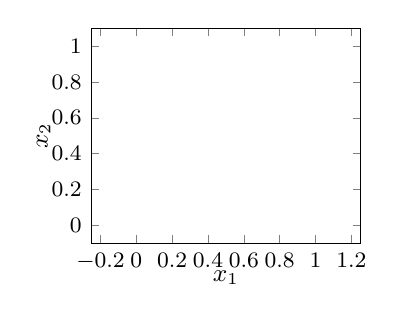
\begin{tikzpicture} 
\begin{axis}[view={\q}{20},axis equal,footnotesize,font=\footnotesize
  ,xlabel={$x_1$},ylabel={$x_2$},zlabel={$x_3$},label shift={-1.5ex} ]
    \threev[right]{2}{-1}{1}{\xv}
    \threev[right]{3.7}{-0.4}{2.3}{\xv'}
%    \threev[right]{1.2}{-1.3}{0.4}{\xv''}
%    \threev[right]{1.7}{-1.1}{0.8}{\xv'''}
\end{axis}
\end{tikzpicture}}
\end{center}


\item To explore further, let's say the second component of~\bv\ is in error by~1\% of~\bv, that is, by~\(0.1\).
As in the previous case, add \((0,0.1,0)\) to the right-hand side and solve to find now \(\xv''=(1.2,-1.3,0.4)\) which is quite different to both~\xv\ and~\(\xv'\), as illustrated below.
Compute its \idx{relative error} \(|\xv-\xv''|/|\xv|=0.43\)\,.
At 43\%, the relative error in solution~\(\xv''\) is also much larger than the 1\%~error in~\bv.
\begin{center}
\qview{-52}{-48}{\begin{tikzpicture} 
\begin{axis}[view={\q}{20},axis equal,footnotesize,font=\footnotesize
  ,xlabel={$x_1$},ylabel={$x_2$},zlabel={$x_3$},label shift={-1.5ex} ]
    \threev[right]{2}{-1}{1}{\xv}
    \threev[right]{3.7}{-0.4}{2.3}{\xv'}
    \node[right] at (axis cs:1.2,-1.3,0.4) {$\xv''$};
    \addplot3[quiver={u=1.2,v=-1.3,w=0.4},blue,-stealth] coordinates {(0,0,0)};
    \node[right] at (axis cs:1.7,-1.1,0.8) {$\xv'''$};
    \addplot3[quiver={u=1.7,v=-1.1,w=0.8},blue,-stealth] coordinates {(0,0,0)};
\end{axis}
\end{tikzpicture}}
\end{center}

\item Lastly, let's say the third component of~\bv\ is in error by~1\% of~\bv, that is, by~\(0.1\).
As in the previous cases, add \((0,0,0.1)\) to the right-hand side and solve to find now \(\xv'''=(1.7,-1.1,0.8)\) which, as illustrated above, is at least is roughly~\xv.
Compute its \idx{relative error} \(|\xv-\xv'''|/|\xv|=0.15\)\,.
At 15\%, the relative error in solution~\(\xv'''\) is significantly larger than the 1\%~error in~\bv.

\end{enumerate}
This example shows that the apparently innocuous matrix~\(A\) variously multiples measurement errors in~\bv\ by factors of at least up to~\(91\) when finding `the solution'~\xv\ to \(A\xv=\bv\)\,.
The matrix~\(A\) must, after all, be a bad matrix.
\cref{thm:erramp} shows this badness is quantified by its  condition number~\(152.27\), and its poor (estimated) reciprocal \(\verb|rcond(A)|=0.0031\). 
\end{example}




\begin{example}  
Consider solving the system of \idx{linear equation}s
\begin{equation*}
\begin{bmatrix} 0.4&0.4&-0.2&0.8
\\-0.2&0.8&-0.4&-0.4
\\0.4&-0.4&-0.8&-0.2
\\-0.8&-0.2&-0.4&0.4 \end{bmatrix}\xv
=\begin{bmatrix} -3\\3\\-9\\-1 \end{bmatrix}.
\end{equation*}
Use \script\ to explore the effect on the solution~\xv\ of 1\%~errors in the right-hand side vector.
\begin{solution} 
Enter the matrix and right-hand side vector into \script, then solve  with \cref{pro:unisol}:
\setbox\ajrqrbox\hbox{\qrcode{% errors
Q=[0.4 0.4 -0.2 0.8
  -0.2 0.8 -0.4 -0.4
  0.4 -0.4 -0.8 -0.2
  -0.8 -0.2 -0.4 0.4]
b=[-3;3;-9;-1]
rcond(Q)
x=Q\slosh b
x1=Q\slosh(b+[0.1;0;0;0])
relerr1=norm(x-x1)/norm(x)
s=svd(Q)
condQ=s(1)/s(4)
}}%
\marginajrbox%
\begin{verbatim}
Q=[0.4 0.4 -0.2 0.8
  -0.2 0.8 -0.4 -0.4
  0.4 -0.4 -0.8 -0.2
  -0.8 -0.2 -0.4 0.4]
b=[-3;3;-9;-1]
rcond(Q)
x=Q\b
\end{verbatim}
to find the solution \(\xv=(-4.6,5,7,-2.2)\).

Now see the effect on this solution of 1\%~errors in~\bv.
Since the length \(|\bv|=\verb|norm(b)|=10\) we find the solution for various changes to~\bv\ of size~\(0.1\).
\begin{itemize}
\item For example, adding the 1\%~error \((0.1,0,0,0)\) to~\bv, the \script\ commands
\begin{verbatim}
x1=Q\(b+[0.1;0;0;0])
relerr1=norm(x-x1)/norm(x)
\end{verbatim}
show the changed solution is \(\xv'=(-4.56,5.04,6.98,-2.12)\) which here is reasonably close to~\xv.
Indeed its relative error \(|\xv-\xv'|/|\xv|\) is computed to be~\(0.0100={}\)1\%.
Here the relative error in solution~\xv\ is exactly the same as the relative error in~\bv.

\item Exploring further, upon adding the 1\%~error \((0,0.1,0,0)\) to~\bv, analogous commands show the changed solution is \(\xv''=(-4.62,5.08,6.96,-2.24)\) which has relative error \(|\xv-\xv''|/|\xv|=0.0100={}\)1\% again.

\item Whereas, upon adding 1\%~error \((0,0,0.1,0)\) to~\bv, analogous commands show the changed solution is \(\xv'''=(-4.56,4.96,6.92,-2.22)\) which has relative error \(|\xv-\xv'''|/|\xv|=0.0100={}\)1\% again.

\item Lastly, upon adding 1\%~error \((0,0,0,0.1)\) to~\bv, analogous commands show the changed solution is \(\xv''''=(-4.68,4.98,6.96,-2.16)\) which has relative error \(|\xv-\xv''''|/|\xv|=0.0100={}\)1\% yet again.

\end{itemize}
In this example, and in contrast to the previous \cref{eg:ilsle}, throughout the relative error in solution~\xv\ is exactly the same as the relative error in~\bv.
The reason is that here the matrix~\(Q\) is an \idx{orthogonal matrix}---check by computing \verb|Q'*Q| (\cref{def:orthog}).
Being orthogonal, multiplication by~\(Q\) only rotates or reflects, and never stretches or distorts (\cref{thm:orthog:i}).
Consequently errors remain the same size when multiplied by such orthogonal matrices, as seen in this example, and as reflected in the condition number of~\(Q\) being one (as computed via \verb|s=svd(Q)| and then \verb|condQ=s(1)/s(4)|).
\end{solution}
\end{example}





The \idx{condition number} determines the reliability of the solution of a system of \idx{linear equation}s.
This is why we should always precede the computation of a solution with an estimate of the condition number such as that provided by the reciprocal~\index{rcond()@\texttt{rcond()}}\verb|rcond()| (\cref{pro:unisol}). 
The next theorem establishes that the condition number characterizes the amplification of errors that occurs in solving a linear system.
Hence solving a system of linear equations with a large condition number (small \verb|rcond|) means that errors are amplified by a large factor as happens in \cref{eg:ilsle}.

\begin{theorem}[error magnification] \label{thm:erramp}
Consider solving \(A\xv=\bv\) for \(n\times n\) matrix~\(A\) with full \(\rank A=n\)\,.  
Suppose the right-hand side \bv~has \idx{relative error} of size~\(\epsilon\), 
\begin{aside}
The symbol~\idx{$\epsilon$} is the Greek letter epsilon, and often denotes errors.
\end{aside}%
then the solution~\xv\ has relative error\({}\leq\epsilon\cond A\)\,, with equality in the worst case.
\end{theorem}

\begin{proof} 
Let the length of the right-hand side vector be \(b=|\bv|\).
Then the error in~\bv\ has size~\(\epsilon b\) since \(\epsilon\)~is the relative error.
Following \cref{pro:gensol},
let \(A=\usv\) be an \svd\ for matrix~\(A\).
Compute \(\zv=\tr U\bv\)\,: recall that multiplication by orthogonal~\(U\) preserves lengths (\cref{thm:orthog}), so not only is \(|\zv|=b\)\,, but also \zv~will be in error by an amount~\(\epsilon b\) since \bv~has this error. 
Consider solving \(S\yv=\zv\)\,: the diagonals of~\(S\) stretch and shrink both the `signal' and the `noise'.
The \emph{worst case} is when \(\zv=(b,0,\ldots,0,\epsilon b)\); that is, when all the `signal' happens to be in the first component of~\zv, and all the `noise', the error, is in the last component.
Then the intermediary \(\yv=(b/\sigma_1,0,\ldots,\epsilon b/\sigma_n)\).
Consequently, the intermediary has relative error \((\epsilon b/\sigma_n)/(b/\sigma_1)=\epsilon(\sigma_1/\sigma_n)=\epsilon\cond A \)\,.
Again because multiplication by orthogonal~\(V\) preserves lengths, the solution \(\xv=V\yv\) has the same relative error:  in the worst case this relative error is~\(\epsilon\cond A\)\,.
\end{proof}

\begin{example} 
Each of the following cases involves solving a linear system \(A\xv=\bv\) to determine quantities of interest~\xv\ from some measured quantities~\bv.
From the given information estimate the \idx{maximum} \idx{relative error} in~\xv,  if  possible, otherwise say so.
\begin{enumerate}
\item Quantities~\bv\ are measured to a relative error~\(0.001\), and matrix~\(A\) has condition number of ten.
\item Quantities~\bv\ are measured to three \idx{significant digits} and \index{rcond()@\texttt{rcond()}}\(\verb|rcond(A)|=0.025\)\,.
\item Measurements are accurate to two \idx{decimal places}, and matrix~\(A\) has condition number of twenty.
\item  Measurements are correct to two significant digits and \(\verb|rcond(A)|=0.002\)\,.
\end{enumerate}

\begin{solution} 
\begin{enumerate}
\item The relative error in~\xv\ could be as big as \(0.001\times10=0.01\)\,.
\item Recall that three significant digits means numbers such as~\(123\) or~\(0.123\) with an error of less than a half of the least significant digit, here~\(0.5\) or~\(0.0005\) respectively.
So measuring to three significant digits means the relative error could be as large as~\(0.005\).
Then here with \(\verb|rcond(A)|=0.025\)\,, matrix~\(A\) has condition number of roughly~\(40\), so the relative error of~\xv\ is less than \(0.005\times40=0.2\)\,; that is, up to~20\%.
\item There is not enough information as we cannot determine the \emph{relative} error in measurements~\bv.
\item Two significant digits means the relative error could be as large as~\(0.05\), whereas matrix~\(A\) has condition number of roughly \(1/0.002=500\) so the relative error of~\xv\ could be as big as \(0.05\times500=25\)\,; that is, the estimated solution~\xv\ is likely to be complete rubbish.
\end{enumerate}
\end{solution}
\end{example}




\begin{activity}
In some experiment the components of~\bv, \(|\bv|=5\)\,, are measured to two \idx{decimal places}.
We compute a vector~\xv\ by solving \(A\xv=\bv\)\,. 
For matrix~\(A\) we compute \index{rcond()@\texttt{rcond()}}\(\verb|rcond(A)|=0.02\)\,.
What is our estimate of the largest possible \idx{relative error} in~\xv?
\actposs[4]{5\%}{20\%}{2\%}{0.1\%}
\end{activity}




This issue of the amplification of errors occurs in other contexts.
The eminent mathematician  \index{Poincar\'e, Henri}Henri Poincar\'e (1854--1912) was the first to detect possible \idx{chaos} in the orbits of the \idx{planets}.
\begin{quoted}{Poincar\'e, 1903}
If we knew exactly the laws of nature and the situation of the universe at the initial moment, we could predict exactly the situation of that same universe at a succeeding moment.
But even if it were the case that the natural laws had no longer any secret for us, we could still only know the initial situation approximately. 
If that enabled us to predict the succeeding situation with the same approximation, that is all we require, and we should say that the phenomenon had been predicted, that it is governed by laws. 
But it is not always so; it may happen that small differences in the \idx{initial condition}s produce very great ones in the final phenomena. 
A small error in the former will produce an enormous error in the latter. 
Prediction becomes impossible, and we have the fortuitous phenomenon.
\end{quoted}
The analogue for us in solving linear equations such as \(A\xv=\bv\) is the following: it may happen that a small error in the elements of~\bv\ will produce an enormous error in the final~\xv.
The condition number warns when this happens by characterizing the amplification. 



\index{condition number|)}

\index{system|)}


\needspace{8\baselineskip}
\subsection{Prove the SVD \cref{thm:svd}}
\label{sec:psvdt}

% Maybe revise in light of the proof by Golub and van Loan p.70

\begin{quoted}{\index{Wiles, Andrew}Andrew Wiles, C1993}
When doing maths there's this great feeling.
You start with a problem that just mystifies you.
You can't understand it, it's so complicated, you just can't make head nor tail of it.
But then when you finally resolve it, you have this incredible feeling of how beautiful it is, how it all fits together so elegantly.
\end{quoted}


\begin{aside}
This proof may be delayed until the last week of a semester.
It may be given together with the closely related classic proof of \cref{thm:smevec} on the eigenvectors of symmetric matrices.  
\end{aside}
Two preliminary examples introduce the structure of the general proof that an \svd\ exists.  
As in this example prelude, the proof of a general singular value decomposition is similarly constructive.

\subsubsection{Prelude to the proof}

These first two examples are optional: their purpose is to introduce two key parts of the general proof in a definite setting.

\begin{example}[a \(2\times2\) case] \label{eg:2by2svdx}
Recall \cref{eg:2by2svd} factorized the matrix
\begin{equation*}
A=\begin{bmatrix} 10&2\\5&11 \end{bmatrix}=
\begin{bmatrix} \frac35&-\frac45\\\frac45&\frac35 \end{bmatrix}
\begin{bmatrix} 10\sqrt2&0\\0&5\sqrt2 \end{bmatrix}
\tr{\begin{bmatrix} \frac1{\sqrt2}&-\frac1{\sqrt2}\\ \frac1{\sqrt2}&\frac1{\sqrt2} \end{bmatrix}}.
\end{equation*}
We find this \idx{factorization}, \(A=\usv\), by maximizing~\(|A\vv|\) over all \idx{unit vector}s~\vv\ (all vectors of length one).


\begin{solution} 
In 2D, all unit vectors are of the form \(\vv=(\cos t,\sin t)\) for \(-\pi<t\leq\pi\)\,.  
The marginal picture plots these unit vectors~\vv\ in blue for 32 angles~\(t\).
\marginpar{\eRose{10/10}{2/10}{5/10}{11/10}}%
\begin{aside}
The \script[1]\ function \index{eigshow()@\texttt{eigshow()}}\texttt{eigshow(A)}\footnote{Download for R2017b and later.} provides an interactive alternative to this static view---click on the \texttt{eig/(svd)} button to make \texttt{eigshow(A)} show \texttt{svd/(eig)}.
\end{aside}%
Plotted in red from the end of each~\vv\ is the vector~\(A\vv\) (scaled down by a factor of ten for clarity).
Our aim is to find the~\vv\ that maximizes the length of the corresponding adjoined~\(A\vv\).
By inspection, the longest red vectors~\(A\vv\) occur towards the top-right or the bottom-left, either of these directions~\vv\ are what we first find.

Maximizing \(|A\vv|\) is the same as maximizing~\(|A\vv|^2\) which is what the following considers: since
\begin{eqnarray*}
A\vv&=&\begin{bmatrix} 10&2\\5&11 \end{bmatrix}
\begin{bmatrix} \cos t\\\sin t \end{bmatrix}
=\begin{bmatrix} 10\cos t+2\sin t\\5\cos t+11\sin t \end{bmatrix},
\\|A\vv|^2&=&(10\cos t+2\sin t)^2+(5\cos t+11\sin t)^2
\\&=&100\cos^2 t+40\cos t\,\sin t+4\sin^2 t
\\&&{}+25\cos^2 t+110\cos t\,\sin t+121\sin^2 t
\\&=&125(\cos^2t+\sin^2t)+150\sin t\,\cos t
\\&=&125+75\sin 2t \qquad(\text{shown in the margin}).
\end{eqnarray*}
\marginpar{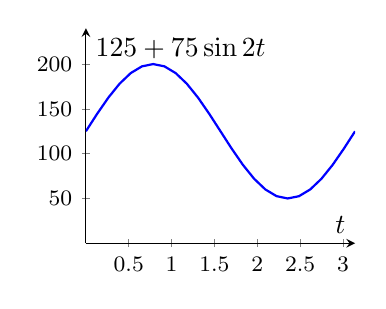
\begin{tikzpicture}
\begin{axis}[footnotesize,axis lines=middle
,xlabel={$t$},ylabel={$125+75\sin 2t$},ymin=0,ymax=240]
\addplot+[thick,no marks,domain=0:3.1415] {125+75*sin(deg(2*\x))};
\end{axis}
\end{tikzpicture}}%
Since the sine function has maximum of one at angle~\(\frac\pi2\)~(\(90^\circ\)), the maximum of~\(|A\vv|^2\) is~\(125+75=200\) for \(2t=\frac\pi2\)\,, that is, for \(t=\frac\pi4\) corresponding to unit vector \(\vv_1=(\cos\frac\pi4,\sin\frac\pi4)=(\frac1{\sqrt2},\frac1{\sqrt2})\)---this vector points to the top-right as identified from the previous marginal figure.
This vector is the first column of~\(V\).

Now multiply to find \(A\vv_1=(6\sqrt2,8\sqrt2)\).  
The length of this vector is \(\sqrt{72+128}=\sqrt{200}=10\sqrt 2=\sigma_1\) the first singular value.  
Normalize the vector~\(A\vv_1\) by \(A\vv_1/\sigma_1 =(6\sqrt2,8\sqrt2)/(10\sqrt2) =(\frac35,\frac45) =\uv_1\)\,, the first column of~\(U\).

The other column of~\(V\) must be orthogonal (at right-angles) to~\(\vv_1\) in order for matrix~\(V\) to be orthogonal.
\marginpar{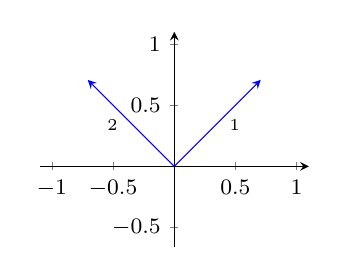
\begin{tikzpicture} 
\begin{axis}[axis equal, axis lines=middle
,footnotesize,font=\footnotesize,xmin=-1.1,xmax=1.1,ymax=1.1 ]
    \addplot[quiver={u=0.707,v=0.707},blue,-stealth] 
    coordinates {(0,0)};
    \node at (axis cs:0.5,0.34) {$\vv_1$};
    \addplot[quiver={u=-0.707,v=0.707},blue,-stealth] 
    coordinates {(0,0)};
    \node at (axis cs:-0.5,0.34) {$\vv_2$};
\end{axis}
\end{tikzpicture}}%
Thus set \(\vv_2=(-\frac1{\sqrt2},\frac1{\sqrt2})\) as shown in the marginal graph.
Now multiply to find \(A\vv_2=(-4\sqrt2,3\sqrt2)\):
magically, and a crucial part of the general proof, the vector~\(A\vv_2\) is orthogonal to~\(\uv_1\).
The length of \(A\vv_2=(-4\sqrt2,3\sqrt2)\) is \(\sqrt{32+18}=\sqrt{50}=5\sqrt2=\sigma_2\), the other singular value.
Normalize the vector to \(A\vv_2/\sigma_2 =(-4\sqrt2,3\sqrt2)/(2\sqrt2)=(-\frac45,\frac35)=\uv_2\)\,, the second column of~\(U\).

This construction establishes that here \(AV=US\)\,. 
Then post-multiply each side by~\(\tr V\) to find an \svd\ is \(A=\usv\).

In this example we could have chosen the negative of~\(\vv_1\) (angle \(t=-\frac{3\pi}4\)), and/or chosen the negative of~\(\vv_2\). 
The result would still be a valid \svd\ of the matrix~\(A\).
The orthogonal matrices in an \svd\ are not unique, and need not be. The singular values are unique.
\end{solution}
\end{example}





\begin{example}[a \(3\times1\) case] \label{eg:3x1svd}
\def\thr{\frac1{\sqrt 3}}
Find the following \svd\ for the \(3\times1\) matrix
\begin{equation*}
A=\begin{bmatrix} 1\\1\\1 \end{bmatrix}
=\begin{bmatrix} \thr&\cdot&\cdot\;
\\\thr&\cdot&\cdot
\\\thr&\cdot&\cdot \end{bmatrix}
\begin{bmatrix} \sqrt3\\0\\0 \end{bmatrix}
\tr{\begin{bmatrix} 1 \end{bmatrix}}=\usv,
\end{equation*}
where we do not worry about the elements denoted by dots as they are multiplied by the zeros in the `diagonal'~\(S=(\sqrt3,0,0)\).
\begin{solution} 
We seek to maximize \(|A\vv|^2\) but, since matrix~\(A\) is \(3\times1\), here vector~\vv\ is in~\(\RR^1\).  
Being of unit magnitude, there are two alternatives: \(\vv=(\pm 1)\). 
Each alternative gives the same \(|A\vv|^2=|(\pm1,\pm1,\pm1)|=3\)\,.  
Choosing one alternative, say \(\vv_1=(1)\), then fixes the matrix \(V=\begin{bmatrix} 1 \end{bmatrix}\).

Then \(A\vv_1=(1,1,1)\) which is of length~\(\sqrt3\).
This length is the singular value \(\sigma_1=\sqrt3\)\,.  
Dividing~\(A\vv_1\) by its length gives the unit vector \(\uv_1=(\thr,\thr,\thr)\), the first column of~\(U\).  
To find the other columns of~\(U\), consider the three standard unit vectors in~\(\RR^3\) (red in the illustration below), rotate them all together so that one lines up with~\(\uv_1\), and then the other two rotated unit vectors form the other two columns of~\(U\) (blue vectors below).  
Since the columns of~\(U\) are then orthonormal, \(U\)~is an orthogonal matrix (\cref{thm:orthog}).
\end{solution}
\begin{center}
\qview{55}{60}{\begin{tikzpicture} 
\begin{axis}[axis equal image,footnotesize,font=\footnotesize,view={\q}{20}]
    \addplot3[quiver={u=1,v=0,w=0},red,-stealth] coordinates {(0,0,0)};
    \addplot3[quiver={u=0,v=1,w=0},red,-stealth] coordinates {(0,0,0)};
    \addplot3[quiver={u=0,v=0,w=1},red,-stealth] coordinates {(0,0,0)};
    \node[left] at (axis cs:1,0,0) {$\vec e_1$};
    \node[below] at (axis cs:0,1,0) {$\vec e_2$};
    \node[right] at (axis cs:0,0,1) {$\vec e_3$};
\threev[above]{0.58}{0.58}{0.58}{\vec u_1}
\threev{0.58}{-0.79}{0.21}{};
\threev{-0.58}{-0.21}{0.79}{};
\end{axis}
\end{tikzpicture}}
\end{center}
\end{example}





\paragraph{Outline of the general proof} 
We use \idx{induction} 
\ifcsname r@sec:pi\endcsname (\cref{sec:pi}) \fi
on the \idx{size} \(m\times n\) of the matrix.
\begin{itemize}
\item First zero matrices have a trivial \svd, and
\(m\times 1\) and \(1\times n\) matrices have a straightforward \svd\ (as in \cref{eg:3x1svd}).
\item For any given \(m\times n\) matrix~\(A\), choose \(\vv_1\) to maximize~\(|A\vv|^2\) among all \idx{unit vector}s \(\vv\) in~\(\RR^n\).
\item Crucially, we then establish that for every vector~\vv\ orthogonal to~\(\vv_1\), the vector \(A\vv\) is orthogonal to~\(A\vv_1\).
\item Then rotate the \idx{standard unit vector}s to align one with~\(\vv_1\). Similarly for~\(A\vv_1\).  
\item This \idx{rotation} transforms the matrix~\(A\) to strip off the leading singular value, and effectively leave an \((m-1)\times(n-1)\) matrix.
\item  By induction on the size, an \svd\ exists for all sizes.
\end{itemize}
This proof corresponds closely to the proof of the spectral \cref{thm:smevec} for symmetric matrices of \cref{sec:sm}. 





\subsubsection{Detailed proof of the SVD \cref{thm:svd}}
\label{sec:dpsvdt}

Use \idx{induction} on the \idx{size} \(m\times n\) of the matrix~\(A\): we assume an \svd\ exists for all \((m-1)\times(n-1)\)~matrices, and prove that consequently an \svd\ must exist for all \(m\times n\)~matrices.  There are three base cases to establish: one for \(m\leq n\)\,, one for \(m\geq n\)\,, and one for matrix \(A=O\)\,; then the induction extends to all sized matrices.

\paragraph{Case $A=O_{m\times n}$:}
When \(m\times n\) matrix \(A=O_{m\times n}\) then choose \(U=I_m\) (orthogonal), \(S=O_{m\times n}\) (diagonal), and \(V=I_n\) (orthogonal) so then \(\usv=I_mO_{m\times n}\tr I_n=O_{m\times n}=A\)\,.  

Consequently, the rest of the proof only considers the non-trivial cases when the matrix~\(A\) is not all zero. 



\paragraph{Case $m\times 1$ ($n=1$):}
Here the \(m\times 1\) nonzero matrix \(A=\begin{bmatrix} \av_1 \end{bmatrix}\) for \(\av_1=(a_{11},a_{21},\ldots,a_{m1})\).
%%%% So far avoided using $\sum$ at all
%Set \(\sigma_1=|\av_1|=\sqrt{\sum_i a_{i1}^2}\) and unit vector \(\uv_1=\av_1/\sigma_1\).
Set the singular value \(\sigma_1=|\av_1|=\sqrt{a_{11}^2+a_{21}^2+\cdots+a_{m1}^2}\) and unit vector \(\uv_1=\av_1/\sigma_1\).
Set \(1\times 1\) orthogonal matrix \(V=\begin{bmatrix} 1 \end{bmatrix}\);
\(m\times 1\) \idx{diagonal matrix} 
%\(S=\begin{bmatrix} \sigma_1\\0\\\vdots\\0 \end{bmatrix}\); and
\(S=(\sigma_1,0,\ldots,0)\); and
\(m\times m\) orthogonal matrix \(U=\begin{bmatrix} \uv_1 &\uv_2&\cdots&\uv_m\end{bmatrix}\).
Matrix~\(U\) exists because we can take the orthonormal set of \idx{standard unit vector}s in~\(\RR^m\) and rotate them all together so that the first lines up with~\(\uv_1\): the other \((m-1)\)~unit vectors then become the other~\(\uv_j\).
Then an \svd\ for the \(m\times1\) matrix~\(A\) is
\begin{eqnarray*}
\usv
&=&\begin{bmatrix} \uv_1 &\uv_2&\cdots&\uv_m\end{bmatrix}
\begin{bmatrix} \sigma_1\\0\\\vdots\\0 \end{bmatrix}
\tr{1}
\\&=&\sigma_1{\uv_1}
=\begin{bmatrix} \av_1 \end{bmatrix}
=A\,.
\end{eqnarray*}

\paragraph{Case $1\times n$ ($m=1$):}
use an exactly complementary argument to the preceding \(m\times1\) case.
%Here \(1\times n\) nonzero matrix \(A=\begin{bmatrix} a_{1j} \end{bmatrix}\).
%Set \(\sigma_1=\sqrt{\sum_j a_{1j}^2}\) and unit vector \(\vv_1=(a_{1i})/\sigma_1\).
%Set \(1\times 1\) orthogonal matrix \(U=\begin{bmatrix} 1 \end{bmatrix}\);
%\(1\times n\) `diagonal' matrix \(S=\begin{bmatrix} \sigma_1&0&\cdots&0 \end{bmatrix}\); and
%\(n\times n\) orthogonal matrix \(V=\begin{bmatrix} \vv_1 &\vv_2&\cdots&\vv_n\end{bmatrix}\).
%Matrix~\(V\) exists because we can take the orthonormal set of standard unit vectors in~\(\RR^n\) and rotate them all together so that the first lines up with~\(\vv_1\): the other \((n-1)\)~unit vectors then become the other~\(\vv_j\).
%Then 
%\(\usv
%=1\begin{bmatrix} \sigma_1&0&\cdots&0 \end{bmatrix}
%\tr{\begin{bmatrix} \vv_1 &\vv_2&\cdots&\vv_n\end{bmatrix}}
%=\sigma_1\tr{\vv_1}
%=\begin{bmatrix} a_{1j} \end{bmatrix}
%=A
%\)



\paragraph{Induction}  
Assume  an \svd\ exists for all \((m-1)\times(n-1)\)~matrices: we proceed to prove that consequently an \svd\ must exist for all \(m\times n\)~matrices.
Consider any \(m\times n\) nonzero matrix~\(A\) with \(m,n\geq2\)\,.
Set vector~\(\vv_1\) in~\(\RR^n\) to be a \emph{unit vector} that maximizes~\(|A\vv|^2\) for unit vectors \(\vv\) in~\(\RR^n\); that is, vector~\(\vv_1\) achieves the \idx{maximum} in \(\max_{|\vv|=1}|A\vv|^2\).
\begin{enumerate}
\item \emph{Such a \idx{maximum} exists by the Extreme Value Theorem in Calculus.}
This theorem is proved in higher level analysis.

%Optional (omit as no real need): confirm that a maximum exists by bounding it.
%Let \(\uv:=A\vv\) so \(u_i=\sum_{n=1}^na_{ij}v_j\)\,.
%Then, upon setting \(a:=\max_{i,j}|a_{ij}|\) and using \(|v_j|\leq1\) as \(|\vv|=1\)\,,
%\begin{equation*}
%|u_i|\leq\sum_{n=1}^n|a_{ij}||v_j|
%\leq\sum_{n=1}^na\cdot1
%=na\,.
%\end{equation*}
%Consequently,
%\begin{equation*}
%|A\vv|^2=|\uv|^2=\sum_{i=1}^m u_i^2
%\leq\sum_{i=1}^m (na)^2 = mn^2a^2.
%\end{equation*}
%Such a bound corresponds to the existence of a maximum of~\(|A\vv|^2\): out of all the any unit vectors that achieve the maximum value, choose any one to be~\(\vv_1\).
%
As matrix~\(A\) is nonzero, there exists~\vv\ such that \(|A\vv|>0\)\,.
Since \(\vv_1\) maximizes \(|A\vv|\) it follows that \(|A\vv_1|>0\)\,.
%Observe that \(|A\vv_1|>0\) as matrix~\(A\) is nonzero.
%Let \(i^*,j^*\) achieve the maximum \(a:=\max_{i,j}|a_{ij}|\)\,: \(a>0\) as the matrix is not all zero. 
%Choosing the unit vector~\(\vv\) to be zero except for a one in the \(j^*\)th~position, the maximum \(|A\vv_1|\geq|A\vv|=|\av_{j^*}|\geq a>0\)\,.

\emph{The vector~\(\vv_1\) is not unique:} for example, the negative~\(-\vv_1\) is another unit vector that achieves the maximum value.  
Sometimes there are other unit vectors that achieve the maximum value. 
Choose any one of them. 

Nonetheless, the maximum value of~\(|A\vv|^2\) is unique, and so the following singular value~\(\sigma_1\) is unique.

\item \emph{Set the singular value \(\sigma_1:=|A\vv_1|>0\) and unit vector \(\uv_1:=(A\vv_1)/\sigma_1\) in~\(\RR^m\). 
For every unit vector~\vv\ orthogonal to~\(\vv_1\) we now prove that the vector~\(A\vv\) is orthogonal to~\(\uv_1\).}
Let \(\uv:=A\vv\) in~\(\RR^m\) and consider \(f(t):=|A(\vv_1\cos t+\vv\sin t)|^2\).
Since \(\vv_1\) achieves the maximum, and \(\vv_1\cos t+\vv\sin t\) is a unit vector for all~\(t\) (\cref{ex:univec}), then \(f(t)\)~must have a maximum at \(t=0\) (maybe at other~\(t\) as well), and so \(f'(0)=0\) (from the Calculus of a maximum).
On the other hand, 
\begin{eqnarray*}
f(t)&=&|A\vv_1\cos t+A\vv\sin t|^2
\\&=&|\sigma_1\uv_1\cos t+\uv\sin t|^2
\\&=&(\sigma_1\uv_1\cos t+\uv\sin t)\cdot(\sigma_1\uv_1\cos t+\uv\sin t)
\\&=&\sigma_1^2\cos^2 t+\sigma_1\uv\cdot\uv_12\sin t\,\cos t+|\uv|^2\sin^2 t
\,;
\end{eqnarray*}
differentiating~\(f(t)\) and evaluating at zero gives
\(f'(0)=\sigma_1\uv\cdot\uv_1\)\,.
As \(t=0\) is a maximum, this derivative is zero, so \(\sigma_1\uv\cdot\uv_1=0\)\,.
Since the singular value \(\sigma_1>0\)\,, we must have \(\uv\cdot\uv_1=0\) and so \(\uv_1\) and~\(\uv\) are orthogonal (\cref{def:orthovec}).

\item Consider the \idx{orthonormal set} of \idx{standard unit vector}s in~\(\RR^n\): rotate them so that the first unit vector lines up with~\(\vv_1\), and let the other \((n-1)\)~rotated unit vectors become the columns of the \(n\times(n-1)\) matrix~\(\bar V\).
Then set the \(n\times n\) matrix
\(V_1:=\begin{bmatrix}\vv_1&\bar V\end{bmatrix}\) which is orthogonal as its columns are orthonormal (\cref{thm:orthog:ii}).
Similarly set an \(m\times m\) \idx{orthogonal matrix}
\(U_1:=\begin{bmatrix}\uv_1&\bar U\end{bmatrix}\).
Compute the \(m\times n\) matrix
\begin{eqnarray*}
A_1:=\tr{U_1}AV_1
&=&\begin{bmatrix} \tr{\uv_1}\\\tr{\bar U} \end{bmatrix}A
\begin{bmatrix} \vv_1 &\bar V \end{bmatrix}
\\&=&\begin{bmatrix} \tr{\uv_1}A\vv_1 & \tr{\uv_1}A\bar V
\\\tr{\bar U}A\vv_1&\tr{\bar U}A\bar V \end{bmatrix}
\end{eqnarray*}
where
\begin{itemize}
\item the top-left entry \(\tr{\uv_1}A\vv_1=\tr{\uv_1}\sigma_1\uv_1=\sigma_1|\uv_1|^2=\sigma_1\)\,,
\item the bottom-left column \(\tr{\bar U}A\vv_1=\tr{\bar U}\sigma_1\uv_1=O_{m-1\times 1}\) as the columns of~\(\bar U\) are orthogonal to~\(\uv_1\),
\item the top-right row \(\tr{\uv_1}A\bar V=O_{1\times n-1}\) as each column of~\(\bar V\) is orthogonal to~\(\vv_1\) and hence each column of~\(A\bar V\) is orthogonal to~\(\uv_1\),
\item and set the bottom-right block \(B:=\tr{\bar U}A\bar V\) which is an \((m-1)\times(n-1)\) matrix as \(\tr{\bar U}\) is~\((m-1)\times m\) and \(\bar V\) is \(n\times(n-1)\).
\end{itemize}
Consequently, 
\begin{equation*}
A_1=\begin{bmatrix} \sigma_1&O_{1\times n-1}
\\O_{m-1\times 1}&B \end{bmatrix}.
\end{equation*}%
Note: rearranging \(A_1:=\tr{U_1}AV_1\) gives \(AV_1=U_1A_1\).

\item \emph{By induction assumption, \((m-1)\times(n-1)\) matrix~\(B\) has an \svd, and so we now construct an \svd\ for \(m\times n\) matrix~\(A\).}
Let \(B=\hat U\hat S\tr{\hat V}\) be an \svd\ for~\(B\).
Then construct (for appropriately sized zero matrices~\(O\))
%\begin{equation*}
%U:=U_1\begin{bmatrix} 1&O_{1\times m-1}\\O_{m-1\times 1}&\hat U \end{bmatrix},\quad
%V:=\begin{bmatrix} 1&O_{1\times n-1}\\O_{n-1\times 1}&\hat V\end{bmatrix}V_1,\quad
%S:=\begin{bmatrix} \sigma_1&O_{1\times n-1}\\O_{m-1\times 1}&\hat S \end{bmatrix}.
%\end{equation*}
\begin{equation*}
U:=U_1\begin{bmatrix} 1&O\\O&\hat U \end{bmatrix},\quad
V:=V_1\begin{bmatrix} 1&O\\O&\hat V\end{bmatrix},\quad
S:=\begin{bmatrix} \sigma_1&O\\O&\hat S \end{bmatrix}.
\end{equation*}
Matrices \(U\) and~\(V\) are orthogonal as each are the product of two orthogonal matrices (\cref{ex:orthoprod}).
Also, matrix~\(S\) is diagonal.
These form an \svd\ for matrix~\(A\) since
\begin{eqnarray*}
AV&=&AV_1\begin{bmatrix} 1&O\\O&\hat V\end{bmatrix}
=U_1A_1\begin{bmatrix} 1&O\\O&\hat V\end{bmatrix}
\\&=&U_1\begin{bmatrix} \sigma_1&O \\O&B \end{bmatrix}\begin{bmatrix} 1&O\\O&\hat V\end{bmatrix}
=U_1\begin{bmatrix} \sigma_1&O \\O&B\hat V \end{bmatrix}
\\&=&U_1\begin{bmatrix} \sigma_1&O \\O&\hat U\hat S \end{bmatrix}
=U_1\begin{bmatrix} 1&O \\O&\hat U \end{bmatrix}
\begin{bmatrix} \sigma_1&O \\O&\hat S \end{bmatrix}
\\&=&US.
\end{eqnarray*}
Hence \(A=\usv\). 
\end{enumerate}
By induction, an \svd\ exists for all \(m\times n\) matrices.
This argument establishes the \svd\ \cref{thm:svd}.







\sectionExercises



\begin{exercise}  
Using a \idx{factorization} of the left-hand side coefficient, quickly solve by hand the following equations.
% p=[2,3,5,7,11]; c=prod(p(ceil(5*rand(1,3)))),b=c*ceil(40+60*rand)
\begin{Parts}
\item \(18 x=1134\)
\begin{reduce}
\item \(42 x=2226\)
\item \(66 x=3234\)
\end{reduce}
\item \(70 x=3150\)
\item \(99 x=8118\)
\begin{reduce}
\item \(154 x=7854\)
\item \(175 x=14350\)
\end{reduce}
\item \(242 x=20086\)
\item \(245 x=12495\)
\begin{reduce}
\item \(363 x=25047\)
\item \(385 x=15785\)
\end{reduce}
\item \(539 x=28028\)
\end{Parts}
\end{exercise}




\begin{exercise} \label{ex:hsledvs} 
Find a \idx{general solution}, if a solution exists, of each of the following systems of \idx{linear equation}s using \cref{pro:gensol}.
Calculate by hand using the given \svd\ factorization; record your working.
% Change any part of this exercise => change a later question.
% u=randq(m), s=diag(-sort(-round(abs(randn(1,4).^2))/2),m,n), v=randq(n), x=v*s'*round(randn(m,1)*4)/2, A=u*s*v', b=A*x
\begin{enumerate}
\item \(\underbrace{\begin{bmatrix} -\frac{9}{5}&\frac{12}{5}
\\-4&-3 \end{bmatrix}}_{=\eAii}\xv
=\begin{bmatrix} -\frac{9}{5}
\\\frac{17}{2} \end{bmatrix}\) given the \svd
\begin{equation*}
\eAii=\begin{bmatrix} 0&1
\\1&0 \end{bmatrix}
\begin{bmatrix} 5&0
\\0&3 \end{bmatrix}
\tr{\begin{bmatrix} -\frac{4}{5}&-\frac{3}{5}
\\-\frac{3}{5}&\frac{4}{5} \end{bmatrix}}
\end{equation*}
\answer{\(\xv=(-1,-\frac{3}{2})\)}

\begin{reduce}
\item \(\underbrace{\begin{bmatrix} \frac{15}{13}&\frac{36}{13}
\\\frac{36}{13}&-\frac{15}{13} \end{bmatrix}}_{=\eAii}\xv
=\begin{bmatrix} \frac{54}{13}
\\-\frac{45}{26} \end{bmatrix}\) given the \svd
\begin{equation*}
\eAii=\begin{bmatrix} -\frac{12}{13}&\frac{5}{13}
\\\frac{5}{13}&\frac{12}{13} \end{bmatrix}
\begin{bmatrix} 3&0
\\0&3 \end{bmatrix}
\tr{\begin{bmatrix} 0&1
\\-1&0 \end{bmatrix}}
\end{equation*}
\answer{\(\xv=(0,\frac{3}{2})\)}

\item \(\underbrace{\begin{bmatrix} -0.96&1.28
\\-0.72&0.96 \end{bmatrix}}_{=\eAii}\xv
=\begin{bmatrix} 2.88
\\2.16 \end{bmatrix}\) given the \svd
\begin{equation*}
\eAii=\begin{bmatrix} \frac{4}{5}&\frac{3}{5}
\\\frac{3}{5}&-\frac{4}{5} \end{bmatrix}
\begin{bmatrix} 2&0
\\0&0 \end{bmatrix}
\tr{\begin{bmatrix} -\frac{3}{5}&-\frac{4}{5}
\\\frac{4}{5}&-\frac{3}{5} \end{bmatrix}}
\end{equation*}
\answer{\(\xv=(-1.08,1.44)-(0.8,0.6)t\)}
\end{reduce}

\item \(\underbrace{\begin{bmatrix} -\frac{5}{26}&-\frac{6}{13}
\\-\frac{12}{13}&\frac{5}{13} \end{bmatrix}}_{=\eAii}\xv
=\begin{bmatrix} -\frac{7}{13}
\\\frac{34}{13} \end{bmatrix}\) given the \svd
\begin{equation*}
\eAii=\begin{bmatrix} 0&1
\\1&0 \end{bmatrix}
\begin{bmatrix} 1&0
\\0&\frac{1}{2} \end{bmatrix}
\tr{\begin{bmatrix} -\frac{12}{13}&-\frac{5}{13}
\\\frac{5}{13}&-\frac{12}{13} \end{bmatrix}}
\end{equation*}
\answer{\(\xv=(-2,2)\)}

\item \(\underbrace{\begin{bmatrix} -\frac{2}{3}&\frac{23}{51}&\frac{22}{51}
\\\frac{1}{6}&\frac{7}{51}&-\frac{31}{51} \end{bmatrix}}_{=\eAii}\xv
=\begin{bmatrix} -\frac{115}{102}
\\-\frac{35}{102} \end{bmatrix}\) given the \svd
\begin{equation*}
\eAii=\begin{bmatrix} \frac{15}{17}&-\frac{8}{17}
\\-\frac{8}{17}&-\frac{15}{17} \end{bmatrix}
\begin{bmatrix} 1&0&0
\\0&\frac{1}{2}&0 \end{bmatrix}
\tr{\begin{bmatrix} -\frac{2}{3}&\frac{1}{3}&-\frac{2}{3}
\\\frac{1}{3}&-\frac{2}{3}&-\frac{2}{3}
\\\frac{2}{3}&\frac{2}{3}&-\frac{1}{3} \end{bmatrix}}
\end{equation*}
\answer{\(\xv=(\frac{10}{9},-\frac{25}{18},\frac{5}{9})-(\frac{2}{3},\frac{2}{3},\frac{1}{3})t\)}

\begin{reduce}
\item \(\underbrace{\begin{bmatrix} \frac{3}{35}&\frac{9}{35}&\frac{9}{70}
\\-\frac{4}{35}&-\frac{12}{35}&-\frac{6}{35} \end{bmatrix}}_{=\eAii}\xv
=\begin{bmatrix} \frac{3}{8}
\\-\frac{1}{2} \end{bmatrix}\) given the \svd
\begin{equation*}
\eAii=\begin{bmatrix} -\frac{3}{5}&\frac{4}{5}
\\\frac{4}{5}&\frac{3}{5} \end{bmatrix}
\begin{bmatrix} \frac{1}{2}&0&0
\\0&0&0 \end{bmatrix}
\tr{\begin{bmatrix} -\frac{2}{7}&-\frac{6}{7}&\frac{3}{7}
\\-\frac{6}{7}&\frac{3}{7}&\frac{2}{7}
\\-\frac{3}{7}&-\frac{2}{7}&-\frac{6}{7} \end{bmatrix}}
\end{equation*}
\answer{\(\xv=(\frac{5}{14},\frac{15}{14},\frac{15}{28})
+(-\frac{6}{7},\frac{3}{7},-\frac{2}{7})s
+(\frac{3}{7},\frac{2}{7},-\frac{6}{7})t\)}

\item \(\underbrace{\begin{bmatrix} \frac{7}{39}&-\frac{17}{39}
\\-\frac{22}{39}&-\frac{19}{39}
\\-\frac{4}{39}&-\frac{53}{78} \end{bmatrix}}_{=\eAii}\xv
=\begin{bmatrix} -\frac{1}{3}
\\-\frac{2}{3}
\\-\frac{2}{3} \end{bmatrix}\) given the \svd
\begin{equation*}
\eAii=\begin{bmatrix} -\frac{1}{3}&\frac{2}{3}&\frac{2}{3}
\\-\frac{2}{3}&-\frac{2}{3}&\frac{1}{3}
\\-\frac{2}{3}&\frac{1}{3}&-\frac{2}{3} \end{bmatrix}
\begin{bmatrix} 1&0
\\0&\frac{1}{2}
\\0&0 \end{bmatrix}
\tr{\begin{bmatrix}\frac{5}{13}&\frac{12}{13}
\\\frac{12}{13}&-\frac{5}{13} \end{bmatrix}}
\end{equation*}
\answer{\(\xv=(\frac{5}{13},\frac{12}{13})\)}
\end{reduce}


\item \(\underbrace{\begin{bmatrix} \frac{36}{119}&-\frac{11}{17}
\\\frac{164}{119}&-\frac{18}{17}
\\-\frac{138}{119}&-\frac{6}{17} \end{bmatrix}}_{=\eAii}\xv
=\begin{bmatrix} \frac{11}{17}
\\\frac{9}{17}
\\\frac{3}{17} \end{bmatrix}\) given the \svd
\begin{equation*}
\eAii=\begin{bmatrix} \frac{2}{7}&-\frac{3}{7}&-\frac{6}{7}
\\\frac{6}{7}&-\frac{2}{7}&\frac{3}{7}
\\-\frac{3}{7}&-\frac{6}{7}&\frac{2}{7} \end{bmatrix}
\begin{bmatrix} 2&0
\\0&1
\\0&0 \end{bmatrix}
\tr{\begin{bmatrix} \frac{15}{17}&\frac{8}{17}
\\-\frac{8}{17}&\frac{15}{17} \end{bmatrix}}
\end{equation*}
\answer{No solution.}

\item \(\underbrace{\begin{bmatrix} -\frac{17}{18}&-\frac{8}{9}&-\frac{8}{9}
\\1&\frac{2}{3}&-\frac{2}{3}
\\-\frac{11}{9}&\frac{8}{9}&-\frac{7}{9} \end{bmatrix}}_{=\eAii}\xv
=\begin{bmatrix} -\frac{17}{18}
\\\frac{5}{3}
\\-\frac{7}{18} \end{bmatrix}\) given the \svd
\begin{equation*}
\eAii=\begin{bmatrix} -\frac{2}{3}&-\frac{1}{3}&-\frac{2}{3}
\\\frac{1}{3}&\frac{2}{3}&-\frac{2}{3}
\\-\frac{2}{3}&\frac{2}{3}&\frac{1}{3} \end{bmatrix}
\begin{bmatrix} 2&0&0
\\0&\frac{3}{2}&0
\\0&0&1 \end{bmatrix}
\tr{\begin{bmatrix} \frac{8}{9}&\frac{1}{9}&-\frac{4}{9}
\\\frac{1}{9}&\frac{8}{9}&\frac{4}{9}
\\\frac{4}{9}&-\frac{4}{9}&\frac{7}{9} \end{bmatrix}}
\end{equation*}
\answer{\(\xv=(1,\frac{1}{2},-\frac{1}{2})\)}

\begin{reduce}
\item \(\underbrace{\begin{bmatrix} -\frac{10}{27}&-\frac{2}{27}&\frac{31}{54}
\\-\frac{4}{27}&\frac{10}{27}&\frac{17}{27}
\\-\frac{8}{27}&-\frac{7}{27}&\frac{7}{27} \end{bmatrix}}_{=\eAii}\xv
=\begin{bmatrix} \frac{83}{54}
\\\frac{49}{54}
\\\frac{17}{54} \end{bmatrix}\) given the \svd
\begin{equation*}
\eAii=\begin{bmatrix} -\frac{2}{3}&\frac{1}{3}&-\frac{2}{3}
\\-\frac{2}{3}&-\frac{2}{3}&\frac{1}{3}
\\-\frac{1}{3}&\frac{2}{3}&\frac{2}{3} \end{bmatrix}
\begin{bmatrix} 1&0&0
\\0&\frac{1}{2}&0
\\0&0&0 \end{bmatrix}
\tr{\begin{bmatrix} \frac{4}{9}&-\frac{4}{9}&\frac{7}{9}
\\-\frac{1}{9}&-\frac{8}{9}&-\frac{4}{9}
\\-\frac{8}{9}&-\frac{1}{9}&\frac{4}{9} \end{bmatrix}}
\end{equation*}
\answer{No solution.}

\item \(\underbrace{\begin{bmatrix} \frac{4}{33}&\frac{4}{11}&\frac{6}{11}
\\\frac{4}{33}&\frac{4}{11}&\frac{6}{11}
\\\frac{2}{33}&\frac{2}{11}&\frac{3}{11} \end{bmatrix}}_{=\eAii}\xv
=\begin{bmatrix} -\frac{7}{3}
\\-\frac{7}{3}
\\-\frac{7}{6} \end{bmatrix}\) given the \svd
\begin{equation*}
\eAii=\begin{bmatrix} \frac{2}{3}&-\frac{2}{3}&\frac{1}{3}
\\\frac{2}{3}&\frac{1}{3}&-\frac{2}{3}
\\\frac{1}{3}&\frac{2}{3}&\frac{2}{3} \end{bmatrix}
\begin{bmatrix} 1&0&0
\\0&0&0
\\0&0&0 \end{bmatrix}
\tr{\begin{bmatrix} \frac{2}{11}&-\frac{9}{11}&\frac{6}{11}
\\\frac{6}{11}&\frac{6}{11}&\frac{7}{11}
\\\frac{9}{11}&-\frac{2}{11}&-\frac{6}{11} \end{bmatrix}}
\end{equation*}
\answer{\(\xv=(-\frac{7}{11},-\frac{21}{11},-\frac{63}{22})+(-\frac{9}{11}.\frac{6}{11},-\frac{2}{11})s+(\frac{6}{11},\frac{7}{11},-\frac{6}{11})t\)}
\end{reduce}

\item \(\underbrace{\begin{bmatrix} -\frac{6}{11}&-\frac{1}{11}&\frac{81}{22}
\\\frac{7}{11}&\frac{3}{11}&\frac{27}{11}
\\-\frac{6}{11}&\frac{9}{22}&-\frac{9}{11} \end{bmatrix}}_{=\eAii}\xv
=\begin{bmatrix} -\frac{35}{2}
\\-\frac{41}{4}
\\\frac{15}{8} \end{bmatrix}\) given the \svd
\begin{equation*}
\eAii=\begin{bmatrix} \frac{9}{11}&\frac{6}{11}&\frac{2}{11}
\\\frac{6}{11}&-\frac{7}{11}&-\frac{6}{11}
\\-\frac{2}{11}&\frac{6}{11}&-\frac{9}{11} \end{bmatrix}
\begin{bmatrix} \frac{9}{2}&0&0
\\0&1&0
\\0&0&\frac{1}{2} \end{bmatrix}
\tr{\begin{bmatrix} 0&-1&0
\\0&0&-1
\\1&0&0 \end{bmatrix}}
\end{equation*}
\answer{\(\xv=(2,-\frac{7}{4},-\frac{9}{2})\)}


\end{enumerate}
\end{exercise}



\begin{exercise} \label{ex:csledvs} 
Find a \idx{general solution}, if a solution exists, of each of the following systems of \idx{linear equation}s.
Calculate by hand using the given \svd\ factorization; check the \svd\ and confirm your calculations with \script\ (\cref{pro:gensol}); then compare and contrast the two methods.
% Change any part of this exercise => change a later exercise.
% u=randq(m), s=diag(-sort(-round(abs(randn(1,4)*2))),m,n), v=randq(n), x=v*s'*round(randn(m,1)*4), A=u*s*v', b=A*x

\arraycolsep=0.2em % gives room for QR-code??
\begin{enumerate}
\item \(\underbrace{\begin{bmatrix} \frac{7}{180}&\frac{8}{45}&\frac{41}{180}
\\\frac{19}{180}&-\frac{22}{45}&\frac{101}{180}
\\-\frac{19}{180}&\frac{4}{45}&\frac{133}{180}
\\\frac{59}{60}&-\frac{2}{15}&\frac{91}{60} \end{bmatrix}}_{=\eAii}\xv
=\begin{bmatrix} -\frac{13}{40}
\\-\frac{9}{8}
\\-\frac{17}{20}
\\-\frac{15}{4} \end{bmatrix}\) given the \svd
\setbox\ajrqrbox\hbox{\qrcode{% SVD
U=[-1 3 3 -9
-3 -9 -1 -3
-3 -1 9 3
-9 3 -3 1]/10
S=[2 0 0
0 1/2 0
0 0 1/2
0 0 0]
V=[-4 4 -7
1 8 4
-8 -1 4]/9
}}%
\marginajrbox%
\begin{equation*}
\eAii=\begin{bmatrix} -\frac{1}{10}&\frac{3}{10}&\frac{3}{10}&-\frac{9}{10}
\\-\frac{3}{10}&-\frac{9}{10}&-\frac{1}{10}&-\frac{3}{10}
\\-\frac{3}{10}&-\frac{1}{10}&\frac{9}{10}&\frac{3}{10}
\\-\frac{9}{10}&\frac{3}{10}&-\frac{3}{10}&\frac{1}{10} \end{bmatrix}
\begin{bmatrix} 2&0&0
\\0&\frac{1}{2}&0
\\0&0&\frac{1}{2}
\\0&0&0 \end{bmatrix}
\tr{\begin{bmatrix} -\frac{4}{9}&\frac{4}{9}&-\frac{7}{9}
\\\frac{1}{9}&\frac{8}{9}&\frac{4}{9}
\\-\frac{8}{9}&-\frac{1}{9}&\frac{4}{9} \end{bmatrix}}
\end{equation*}
\answer{\(\xv=(-\frac{19}{12},\frac{1}{3},-\frac{17}{12})\)}


\begin{reduce}
\item \(\underbrace{\begin{bmatrix} \frac{79}{66}&\frac{7}{33}&-\frac{29}{33}
\\-\frac{65}{66}&-\frac{13}{33}&\frac{35}{33}
\\\frac{31}{66}&-\frac{29}{33}&-\frac{37}{33}
\\\frac{17}{66}&-\frac{23}{33}&-\frac{43}{33} \end{bmatrix}}_{=\eAii}\xv
=\begin{bmatrix} -\frac{22}{6}
\\\frac{20}{6}
\\-\frac{1}{6}
\\\frac{1}{6} \end{bmatrix}\) given the \svd
\setbox\ajrqrbox\hbox{\qrcode{% SVD
U=[-1 -1 -1 -1
1 1 -1 -1
-1 1 -1 1
-1 1 1 -1]/2
S=[8 0 0
0 4 0
0 0 1
0 0 0]/3
V=[-6 -6 -7
2 -9 6
9 -2 -6]/11
}}%
\marginajrbox%
\begin{equation*}
\eAii=\begin{bmatrix} -\frac{1}{2}&-\frac{1}{2}&-\frac{1}{2}&-\frac{1}{2}
\\\frac{1}{2}&\frac{1}{2}&-\frac{1}{2}&-\frac{1}{2}
\\-\frac{1}{2}&\frac{1}{2}&-\frac{1}{2}&\frac{1}{2}
\\-\frac{1}{2}&\frac{1}{2}&\frac{1}{2}&-\frac{1}{2} \end{bmatrix}
\begin{bmatrix} \frac{8}{3}&0&0
\\0&\frac{4}{3}&0
\\0&0&\frac{1}{3}
\\0&0&0 \end{bmatrix}
\tr{\begin{bmatrix} -\frac{6}{11}&-\frac{6}{11}&-\frac{7}{11}
\\\frac{2}{11}&-\frac{9}{11}&\frac{6}{11}
\\\frac{9}{11}&-\frac{2}{11}&-\frac{6}{11} \end{bmatrix}}
\end{equation*}
\answer{No solution.}


\item \(\underbrace{\begin{bmatrix} \frac{14}{15}&-\frac{14}{15}&\frac{7}{15}&-\frac{28}{15}
\\\frac{2}{5}&-\frac{8}{5}&-\frac{4}{5}&\frac{4}{5}
\\-\frac{6}{5}&-\frac{6}{5}&\frac{12}{5}&\frac{3}{5} \end{bmatrix}}_{=\eAii}\xv
=\begin{bmatrix} 0
\\4
\\27 \end{bmatrix}\) given the \svd
\setbox\ajrqrbox\hbox{\qrcode{% SVD
U=[0 -1 0
0 0 -1
-1 0 0]
S=[3 0 0 0
0 7/3 0 0
0 0 2 0]
V=[2 -2 -1 4
2 2 4 1
-4 -1 2 2
-1 4 -2 2]/5
}}%
\marginajrbox%
\begin{equation*}
\eAii=\begin{bmatrix} 0&-1&0
\\0&0&-1
\\-1&0&0 \end{bmatrix}
\begin{bmatrix} 3&0&0&0
\\0&\frac{7}{3}&0&0
\\0&0&2&0 \end{bmatrix}
\tr{\begin{bmatrix} \frac{2}{5}&-\frac{2}{5}&-\frac{1}{5}&\frac{4}{5}
\\\frac{2}{5}&\frac{2}{5}&\frac{4}{5}&\frac{1}{5}
\\-\frac{4}{5}&-\frac{1}{5}&\frac{2}{5}&\frac{2}{5}
\\-\frac{1}{5}&\frac{4}{5}&-\frac{2}{5}&\frac{2}{5} \end{bmatrix}}
\end{equation*}
\answer{\(\xv=(-\frac{16}{5},-\frac{26}{5},\frac{32}{5},\frac{13}{5})
+(\frac{4}{5},\frac{1}{5},\frac{2}{5},\frac{2}{5})t\)}
\end{reduce}


\item \(\underbrace{\begin{bmatrix} \frac{57}{22}&-\frac{3}{22}&-\frac{45}{22}&-\frac{9}{22}
\\-\frac{14}{11}&\frac{32}{11}&-\frac{4}{11}&-\frac{14}{11}
\\-\frac{9}{22}&-\frac{3}{22}&-\frac{45}{22}&\frac{57}{22} \end{bmatrix}}_{=\eAii}\xv
=\begin{bmatrix} 117
\\-72
\\63 \end{bmatrix}\) given the \svd
\setbox\ajrqrbox\hbox{\qrcode{% SVD
U=[-6 9 2
7 6 -6
-6 -2 -9]/11
S=[4 0 0 0
0 3 0 0
0 0 3 0]
V=[-1 1 1 1
1 1 -1 1
1 -1 1 1
-1 -1 -1 1]/2
}}%
\marginajrbox%
\begin{equation*}
\eAii=\begin{bmatrix} -\frac{6}{11}&\frac{9}{11}&\frac{2}{11}
\\\frac{7}{11}&\frac{6}{11}&-\frac{6}{11}
\\-\frac{6}{11}&-\frac{2}{11}&-\frac{9}{11} \end{bmatrix}
\begin{bmatrix} 4&0&0&0
\\0&3&0&0
\\0&0&3&0 \end{bmatrix}
\tr{\begin{bmatrix} -\frac{1}{2}&\frac{1}{2}&\frac{1}{2}&\frac{1}{2}
\\\frac{1}{2}&\frac{1}{2}&-\frac{1}{2}&\frac{1}{2}
\\\frac{1}{2}&-\frac{1}{2}&\frac{1}{2}&\frac{1}{2}
\\-\frac{1}{2}&-\frac{1}{2}&-\frac{1}{2}&\frac{1}{2} \end{bmatrix}}
\end{equation*}
\answer{\(\xv=(27,-12,-24,9)
+(\frac{1}{2},\frac{1}{2},\frac{1}{2},\frac{1}{2})t\)}


\item \(\underbrace{\begin{bmatrix} -\frac{2}{5}&-\frac{2}{5}&-\frac{26}{45}&\frac{26}{45}
\\\frac{11}{9}&\frac{11}{9}&-\frac{1}{3}&\frac{1}{3}
\\\frac{31}{90}&\frac{31}{90}&\frac{17}{90}&-\frac{17}{90}
\\\frac{4}{9}&\frac{4}{9}&-\frac{2}{9}&\frac{2}{9} \end{bmatrix}}_{=\eAii}\xv
=\begin{bmatrix} 3\\-6\\-3\\-2 \end{bmatrix}\) given the \svd
\setbox\ajrqrbox\hbox{\qrcode{% SVD
U=[2 8 3 2
-8 2 -2 3
-2 -3 8 2
-3 2 2 -8]/9
S=[2 0 0 0
0 1 0 0
0 0 0 0
0 0 0 0]
V=[-7 -1 1 -7
-7 -1 -1 7
1 -7 -7 -1
-1 7 -7 -1]/10
}}%
\marginajrbox%
\begin{equation*}
\eAii=\begin{bmatrix} \frac{2}{9}&\frac{8}{9}&\frac{1}{3}&\frac{2}{9}
\\-\frac{8}{9}&\frac{2}{9}&-\frac{2}{9}&\frac{1}{3}
\\-\frac{2}{9}&-\frac{1}{3}&\frac{8}{9}&\frac{2}{9}
\\-\frac{1}{3}&\frac{2}{9}&\frac{2}{9}&-\frac{8}{9} \end{bmatrix}
\begin{bmatrix} 2&0&0&0
\\0&1&0&0
\\0&0&0&0
\\0&0&0&0 \end{bmatrix}
\tr{\begin{bmatrix} -\frac{7}{10}&-\frac{1}{10}&\frac{1}{10}&-\frac{7}{10}
\\-\frac{7}{10}&-\frac{1}{10}&-\frac{1}{10}&\frac{7}{10}
\\\frac{1}{10}&-\frac{7}{10}&-\frac{7}{10}&-\frac{1}{10}
\\-\frac{1}{10}&\frac{7}{10}&-\frac{7}{10}&-\frac{1}{10} \end{bmatrix}}
\end{equation*}
\answer{No solution.}


\begin{reduce}
\item \(\underbrace{\begin{bmatrix} \frac{5}{14}&-\frac{41}{14}&\frac{1}{2}&-\frac{3}{2}
\\\frac{22}{7}&-\frac{4}{7}&0&2
\\-\frac{9}{14}&-\frac{13}{14}&\frac{5}{2}&-\frac{1}{2}
\\-\frac{2}{7}&-\frac{6}{7}&2&2 \end{bmatrix}}_{=\eAii}\xv
=\begin{bmatrix} -45
\\-50
\\18
\\20 \end{bmatrix}\) given the \svd
\setbox\ajrqrbox\hbox{\qrcode{% SVD
U=[4 2 -5 2
-4 5 -2 -2
4 2 2 -5
1 4 4 4]/7
S=[4 0 0 0
0 4 0 0
0 0 3 0
0 0 0 1]
V=[-1 1 -1 -1
-1 -1 1 -1
1 1 1 -1
-1 1 1 1]/2
}}%
\marginajrbox%
\begin{equation*}
\eAii=\begin{bmatrix} \frac{4}{7}&\frac{2}{7}&-\frac{5}{7}&\frac{2}{7}
\\-\frac{4}{7}&\frac{5}{7}&-\frac{2}{7}&-\frac{2}{7}
\\\frac{4}{7}&\frac{2}{7}&\frac{2}{7}&-\frac{5}{7}
\\\frac{1}{7}&\frac{4}{7}&\frac{4}{7}&\frac{4}{7} \end{bmatrix}
\begin{bmatrix} 4&0&0&0
\\0&4&0&0
\\0&0&3&0
\\0&0&0&1 \end{bmatrix}
\tr{\begin{bmatrix} -\frac{1}{2}&\frac{1}{2}&-\frac{1}{2}&-\frac{1}{2}
\\-\frac{1}{2}&-\frac{1}{2}&\frac{1}{2}&-\frac{1}{2}
\\\frac{1}{2}&\frac{1}{2}&\frac{1}{2}&-\frac{1}{2}
\\-\frac{1}{2}&\frac{1}{2}&\frac{1}{2}&\frac{1}{2} \end{bmatrix}}
\end{equation*}
\answer{\(\xv=(-\frac{33}{2},\frac{25}{2},\frac{17}{2},\frac{9}{2})\)}
\end{reduce}


\end{enumerate}
\end{exercise}



\begin{exercise}  
Find a \idx{general solution}, if possible, of each of the following systems of \idx{linear equation}s with \script\ and using \cref{pro:gensol}.
\begin{enumerate}
\itemsep=3ex %more space for QR codes??
% u=randq(m), s=diag(-sort(-round(abs(randn(1,min(m,n))*3))),m,n), v=randq(n), x=round(randn(n,1)*4), A=u*s*v', b=A*x
\item \(\begin{bmatrix} 2.4&1.6&1&-0.8
\\-1.2&3.2&-2&-0.4
\\-1.2&-0.8&2&-1.6
\\0.6&-1.6&-4&-0.8 \end{bmatrix}\xv
=\begin{bmatrix} -29.4
\\-12.4
\\13.2
\\-0.8 \end{bmatrix}\)
\setbox\ajrqrbox\hbox{\qrcode{% Ax=b
A=[2.4 1.6 1 -0.8
-1.2 3.2 -2 -0.4
-1.2 -0.8 2 -1.6
0.6 -1.6 -4 -0.8]
b=[-29.4;-12.4;13.2;-0.8]
}}%
\marginajrbox%
\answer{\(\xv=(-8,-6,1,2)\)}


\begin{reduce}
\item \(\begin{bmatrix} -0.7&-0.7&-2.5&-0.7
\\1&-2.2&0.2&-0.2
\\-1&1.4&-1.4&-2.6
\\2.6&-1.4&-1&-1.4 \end{bmatrix}\xv
=\begin{bmatrix} -4
\\2.4
\\3.2
\\0 \end{bmatrix}\)
\setbox\ajrqrbox\hbox{\qrcode{% Ax=b
A=[-0.7 -0.7 -2.5 -0.7
1 -2.2 0.2 -0.2
-1 1.4 -1.4 -2.6
2.6 -1.4 -1 -1.4]
b=[-4;2.4;3.2;0]
}}%
\marginajrbox%
\answer{\(\xv=(-1,-1,3,-3)\)}


\item \(\begin{bmatrix} -3.14&-1.18&0.46&-0.58
\\0.66&0.18&-0.06&2.22
\\-1.78&-2.54&-1.82&-5.26
\\0.58&1.06&-0.82&0.26 \end{bmatrix}\xv
=\begin{bmatrix} -17.38
\\-1.14
\\5.22
\\12.26 \end{bmatrix}\)
\setbox\ajrqrbox\hbox{\qrcode{% Ax=b
A=[-3.14 -1.18 0.46 -0.58
0.66 0.18 -0.06 2.22
-1.78 -2.54 -1.82 -5.26
0.58 1.06 -0.82 0.26]
b=[-17.38;-1.14;5.22;12.26]
}}%
\marginajrbox%
\answer{\(\xv=(3,5,-7,-2)\)}
\end{reduce}


\item \(\begin{bmatrix} 1.38&0.50&3.30&0.34
\\-0.66&-0.70&1.50&-2.38
\\-0.90&2.78&-0.54&0.10
\\0.00&1.04&-0.72&-1.60 \end{bmatrix}\xv
=\begin{bmatrix} -7.64
\\-7.72
\\-20.72
\\-20.56 \end{bmatrix}\)
\setbox\ajrqrbox\hbox{\qrcode{% Ax=b
A=[1.38 0.50 3.30 0.34
-0.66 -0.70 1.50 -2.38
-0.90 2.78 -0.54 0.10
0.00 1.04 -0.72 -1.60]
b=[-7.64;-7.72;-20.72;-20.56]
}}%
\marginajrbox%
\answer{\(\xv=(-4,-9,0,7)\)}


\item \(\begin{bmatrix} 1.32&1.40&1.24&-0.20
\\1.24&3.00&2.68&1.00
\\1.90&-1.06&-1.70&2.58
\\-1.30&0.58&0.90&-0.94 \end{bmatrix}\xv
=\begin{bmatrix} -5.28
\\2.04
\\6.30
\\2.50 \end{bmatrix}\)
\setbox\ajrqrbox\hbox{\qrcode{% Ax=b
A=[1.32 1.40 1.24 -0.20
1.24 3.00 2.68 1.00
1.90 -1.06 -1.70 2.58
-1.30 0.58 0.90 -0.94]
b=[-5.28;2.04;6.30;2.50]
}}%
\marginajrbox%
\answer{No solution.}

% u=randq(m), s=diag(-sort(-round(abs(randn(1,min(m,n))*2))),m,n), v=randq(n), x=v*s'*round(randn(m,1)*4), A=u*s*v', b=A*x
\begin{reduce}
\item \(\begin{bmatrix} 2.16&0.82&-2.06&0.72
\\-0.18&-0.56&1.84&-0.78
\\1.68&-0.14&0.02&-0.24
\\-1.14&-0.88&-2.48&0.66 \end{bmatrix}\xv
=\begin{bmatrix} -12.6
\\13.8
\\0.2
\\-32.6 \end{bmatrix}\)
\setbox\ajrqrbox\hbox{\qrcode{% Ax=b
A=[2.16 0.82 -2.06 0.72
-0.18 -0.56 1.84 -0.78
1.68 -0.14 0.02 -0.24
-1.14 -0.88 -2.48 0.66]
b=[-12.6;13.8;0.2;-32.6]
}}%
\marginajrbox%
\answer{\(\xv=(0.6,8.2,9.8,-0.6)
+(-0.1,0.3,-0.3,-0.9)t\)}


\item \(\begin{bmatrix} 0.00&-0.54&-0.72&0.90
\\0.40&0.74&0.32&-0.10
\\1.20&2.22&0.96&-0.30
\\-0.00&-0.18&-0.24&0.30 \end{bmatrix}\xv
=\begin{bmatrix} -1.8
\\-3.2
\\-9.6
\\-0.6 \end{bmatrix}\)
\setbox\ajrqrbox\hbox{\qrcode{% Ax=b
A=[0.00 -0.54 -0.72 0.90
0.40 0.74 0.32 -0.10
1.20 2.22 0.96 -0.30
-0.00 -0.18 -0.24 0.30]
b=[-1.8;-3.2;-9.6;-0.6]
}}%
\marginajrbox%
\answer{\(\xv=(-3.2,-3.4,0.8,-3.4)
+(0.8,-0.4,-0.2,-0.4)s
+(0.2,-0.4,0.8,0.4)t\)}
\end{reduce}

% m=ceil(rand*3)+2;n=ceil(rand*3)+2; a=round(randn(m,n)*3)+0, x=round(randn(1,n)*30)/10+0, b=a*x', svs=svd(a)'
\item \(\begin{bmatrix} 7&1&-1&4
\\2&4&-4&0
\\0&4&0&-1
\\-4&1&1&-1
\\-1&0&-1&3 \end{bmatrix}\xv
=\begin{bmatrix} 22.4\\11.2\\-6.1\\-8.3\\17.8 \end{bmatrix}\)
\setbox\ajrqrbox\hbox{\qrcode{% Ax=b
A=[7 1 -1 4
2 4 -4 0
0 4 0 -1
-4 1 1 -1
-1 0 -1 3]
b=[22.4;11.2;-6.1;-8.3;17.8]
}}%
\marginajrbox%
\answer{\(\xv=(0,-0.3,-3.1,4.9)\)}


\item \(\begin{bmatrix} 7&1&-1&4
\\2&4&-4&0
\\0&4&0&-1
\\-4&1&1&-1
\\-1&0&-1&3 \end{bmatrix}\xv
=\begin{bmatrix} -2.1\\2.2\\4.6\\-0.7\\5.5 \end{bmatrix}\)
\setbox\ajrqrbox\hbox{\qrcode{% Ax=b
A=[7 1 -1 4
2 4 -4 0
0 4 0 -1
-4 1 1 -1
-1 0 -1 3]
b=[-2.1;2.2;4.6;-0.7;5.5]
}}%
\marginajrbox%
\answer{No solution.}


\begin{reduce}
\item \(\begin{bmatrix} -1&0&-6&0&5
\\0&-3&2&1&7
\\0&2&-3&-2&2
\\0&-3&7&-5&0 \end{bmatrix}\xv
=\begin{bmatrix} 30.7
\\-17.0
\\21.3
\\-45.7 \end{bmatrix}\)
\setbox\ajrqrbox\hbox{\qrcode{% Ax=b
A=[-1 0 -6 0 5
0 -3 2 1 7
0 2 -3 -2 2
0 -3 7 -5 0]
b=[30.7;-17.0;21.3;-45.7]
}}%
\marginajrbox%
\answer{\(\xv=(0.18,3.35,-4.86,0.33,0.35)
\)\\\({}
+(0.91,-0.34,-0.21,-0.09,-0.07)t\) \twodp}


\item \(\begin{bmatrix} 1&6&1&1&-4
\\3&-2&0&-4&7
\\1&-3&-1&-5&-2
\\-1&4&-2&-1&-2 \end{bmatrix}\xv
=\begin{bmatrix} 4
\\-7
\\2
\\-3 \end{bmatrix}\)
\setbox\ajrqrbox\hbox{\qrcode{% Ax=b
A=[1 6 1 1 -4
3 -2 0 -4 7
1 -3 -1 -5 -2
-1 4 -2 -1 -2]
b=[4;-7;2;-3]
}}%
\marginajrbox%
\answer{\(\xv=(0.70,-0.54,1.16,0.34,-1.26)
\)\\\({}
+(-0.64,0.12,0.66,-0.37,0.10)t\) \twodp}
\end{reduce}


%\item \(\begin{bmatrix}  \end{bmatrix}\xv
%=\begin{bmatrix}  \end{bmatrix}\)
%\setbox\ajrqrbox\hbox{\qrcode{% Ax=b
%A=[]
%b=[]
%}}%
%\marginajrbox%
%\answer{\(\xv=()\)}
%
%
\end{enumerate}
\end{exercise}




\begin{exercise}  
Recall \cref{thm:fred,thm:feweqns} on the existence of none, one, or an infinite number of solutions to \idx{linear equation}s.
Use \cref{pro:gensol} to provide an alternative proof to each of these two theorems.
\end{exercise}





\begin{exercise}  
Write down the \idx{condition number} and the \idx{rank} of each of the matrices in \cref{ex:hsledvs} using the given \svd{}s.
\answer{\protect\begin{enumerate}[label=(\protect\alph*)]
\protect\item{}cond\({}=5/3\),  rank\({}=2\);
\protect\begin{reduce}
\protect\item{}cond\({}=1\),  rank\({}=2\);
\protect\item{}cond\({}=\infty\),  rank\({}=1\);
\protect\end{reduce}
\protect\item{}cond\({}=2\),  rank\({}=2\);
\protect\item{}cond\({}=2\),  rank\({}=2\);
\protect\begin{reduce}
\protect\item{}cond\({}=\infty\),  rank\({}=1\);
\protect\item{}cond\({}=2\),  rank\({}=2\);
\protect\end{reduce}
\protect\item{}cond\({}=2\),  rank\({}=2\);
\protect\item{}cond\({}=2\),  rank\({}=3\);
\protect\begin{reduce}
\protect\item{}cond\({}=\infty\),  rank\({}=2\);
\protect\item{}cond\({}=\infty\),  rank\({}=1\);
\protect\end{reduce}
\protect\item{}cond\({}=9\),  rank\({}=3\);
\protect\end{enumerate}}
\end{exercise}




\begin{reduce}
\begin{exercise}  
Write down the \idx{condition number} and the \idx{rank} of each of the matrices in \cref{ex:csledvs} using the given \svd{}s.
For each square matrix, compute \verb|rcond| and comment on its relation to the \idx{condition number}.
\answer{Since the \protect\verb|rcond| function uses heuristics, it may differ depending upon the software version.
\protect\begin{enumerate}[label=(\protect\alph*)]
\protect\item{}cond\({}=4\), rank\({}=3\), \protect\verb|rcond| dne;
\protect\item{}cond\({}=8\), rank\({}=3\), \protect\verb|rcond| dne;
\protect\item{}cond\({}=3/2\), rank\({}=3\), \protect\verb|rcond| dne;
\protect\item{}cond\({}=4/3\), rank\({}=3\), \protect\verb|rcond| dne;
\protect\item{}cond\({}=\infty\), rank\({}=2\), \protect\verb|rcond|\({}=0\);
\protect\item{}cond\({}=4\), rank\({}=4\), \protect\verb|rcond|\({}=0.1167\).
\protect\end{enumerate}}
\end{exercise}
\end{reduce}



\begin{exercise}  
In \script, use \verb|randn()| to generate some random matrices~\(A\) of chosen sizes, and some correspondingly sized random right-hand side vectors~\bv.
For each, find a \idx{general solution}, if possible, of the system \(A\xv=\bv\) with \script\ and using \cref{pro:gensol}.
Record each step, the \idx{condition number} and rank of~\(A\), and comment on what is interesting about the sizes you choose.
\end{exercise}


\begin{exercise} \label{ex:svdtrAA} 
Let \(m\times n\) matrix~\(A\) have the \svd\ \(A=\usv\).
Derive that the matrix \(\tr AA\) has an \svd\ \(\tr AA=V\bar S\tr V\), for what matrix~\(\bar S\)?
Derive that the matrix \(A\tr A\) has an \svd\ \(A\tr A=U\tilde S\tr U\), for what matrix~\(\tilde S\)?
\end{exercise}




\begin{exercise}  
Consider the problems in \cref{ex:hsledvs,ex:csledvs}.
For each of these problems comment on the applicability of the Unique Solution \cref{thm:ftim1}, and comment on how the solution(s) illustrate the theorem.
\answer{The theorem applies to the square matrix systems of \cref{ex:hsledvs,ex:csledvs}.
The cases with no zero singular value, full rank, have a unique solution.
The cases with a zero singular value, rank less than~\(n\), either have no solution or an infinite number.}
\end{exercise}



\begin{exercise}  
Recall \cref{def:invertible} says that a square matrix~\(A\) is \idx{invertible} if there exists a matrix~\(B\) such that \emph{both} \(AB=I\) \emph{and} \(BA=I\)\,.
We now see that we need only one of these to ensure the matrix is invertible.
\begin{enumerate}
\item Use \cref{thm:ftim1iii} to now prove that a square matrix~\(A\) is invertible if there exists a matrix~\(B\) such that \(BA=I\)\,.

\item Use the transpose and \cref{thm:ftim1v,thm:ranktr} to then prove that a square matrix~\(A\) is invertible if there exists a matrix~\(B\) such that \(AB=I\)\,.
\end{enumerate}
\end{exercise}




\begin{exercise}  
For each of the following systems, explore the effect on the solution of 1\%~errors in the right-hand side, and comment on the relation to the given \idx{condition number} of the matrix.
% for i=1:999, A=round(randn(2)*4)+0; if prod(abs(det(A))-[1,2,5,10])==0 & cond(A)<3, detA=det(A),condA=cond(A),[U,S,V]=svd(A); b=round(10*U(:,1)), break, end,end

\begin{enumerate}
\begin{reduce}
\item \(\begin{bmatrix} 1&0
\\-4&1 \end{bmatrix}\xv
=\begin{bmatrix} -2
\\10 \end{bmatrix}\), 
\(\cond=17.94\)
\end{reduce}

\item \(\begin{bmatrix} 2&-4
\\-2&-1 \end{bmatrix}\xv
=\begin{bmatrix} 10
\\0 \end{bmatrix}\), 
\(\cond=2\)

\item \(\begin{bmatrix} -3&1
\\-4&2 \end{bmatrix}\xv
=\begin{bmatrix} 6\\8 \end{bmatrix}\), 
\(\cond=14.93\)

\item \(\begin{bmatrix} -1&1
\\4&-5 \end{bmatrix}\xv
=\begin{bmatrix} -2
\\10 \end{bmatrix}\), 
\(\cond=42.98\)

\begin{reduce}
\item \(\begin{bmatrix} -1&-2
\\3&1 \end{bmatrix}\xv
=\begin{bmatrix} -5
\\9 \end{bmatrix}\), 
\(\cond=2.618\)
\end{reduce}

\end{enumerate}
\end{exercise}



\begin{exercise}  
For each of the following systems, use \script\ to explore the effect on the solution of \(0.1\)\%~errors in the right-hand side.
Record your commands and output, and comment on the relation to the  condition number of the matrix.
% for i=1:9999, A=round(randn(4)*5)+0; if abs(prod(abs(det(A))-[1,2,5,10,20,50,100]))<1e-7 & cond(A)>400, detA=det(A),condA=cond(A),[U,S,V]=svd(A); b=round(10*U(:,1))+0, break, end,end

\begin{enumerate}
%\itemsep=5ex

\item \(\begin{bmatrix} 1&2&2
\\-1&-1&0
\\0&3&1 \end{bmatrix}\xv
=\begin{bmatrix} -7
\\2
\\-7 \end{bmatrix}\)
\setbox\ajrqrbox\hbox{\qrcode{% system
A=[1 2 2
 -1 -1 0
 0 3 1]
b=[-7
 2
 -7]
}}%
\marginajrbox%

\begin{reduce}
\item \(\begin{bmatrix} -1&6&-1
\\0&1&3
\\-1&7&3 \end{bmatrix}\xv
=\begin{bmatrix} 6
\\2
\\8 \end{bmatrix}\)
\setbox\ajrqrbox\hbox{\qrcode{% system
A=[-1 6 -1
 0 1 3
 -1 7 3]
b=[6
 2
 8]
}}%
\marginajrbox%

\item \(\begin{bmatrix} 1&3&4&0
\\0&0&-5&5
\\3&1&0&8
\\1&2&1&5 \end{bmatrix}\xv
=\begin{bmatrix} 0
\\5
\\7
\\4 \end{bmatrix}\)
\setbox\ajrqrbox\hbox{\qrcode{% system
A=[1 3 4 0
 0 0 -5 5
 3 1 0 8
 1 2 1 5]
b=[0
 5
 7
 4]
}}%
\marginajrbox%
\end{reduce}

\item \(\begin{bmatrix} -3&-2&-2&-2
\\2&1&-5&-7
\\2&4&3&3
\\2&1&1&1 \end{bmatrix}\xv
=\begin{bmatrix} -3
\\-8
\\5
\\2 \end{bmatrix}\)
\setbox\ajrqrbox\hbox{\qrcode{% system
A=[-3 -2 -2 -2
 2 1 -5 -7
 2 4 3 3
 2 1 1 1]
b=[-3
 -8
 5
 2]
}}%
\marginajrbox%

% for i=1:9999, A=round(randn(5)*5)+0; if cond(A)>1000, detA=det(A),condA=cond(A),[U,S,V]=svd(A); b=round(10*U(:,1))+0, break, end,end

\item \(\begin{bmatrix} -1&6&-6&2&7
\\-7&4&3&1&-8
\\7&6&4&0&5
\\-8&3&3&2&4
\\2&0&-3&1&0 \end{bmatrix}\xv
=\begin{bmatrix} 5
\\-7
\\5
\\-2
\\1 \end{bmatrix}\)
\setbox\ajrqrbox\hbox{\qrcode{% system
A=[-1 6 -6 2 7
 -7 4 3 1 -8
 7 6 4 0 5
 -8 3 3 2 4
 2 0 -3 1 0]
b=[5
 -7
 5
 -2
 1]
}}%
\marginajrbox%

\begin{reduce}
\item \(\begin{bmatrix} 9&0&-10&-8&-1
\\9&3&-5&-4&4
\\-1&0&-3&-6&-6
\\4&6&0&-5&-14
\\-2&-1&-4&-7&5 \end{bmatrix}\xv
=\begin{bmatrix} 7
\\4
\\3
\\5
\\1 \end{bmatrix}\)
\setbox\ajrqrbox\hbox{\qrcode{% system
A=[9 0 -10 -8 -1
 9 3 -5 -4 4
 -1 0 -3 -6 -6
 4 6 0 -5 -14
 -2 -1 -4 -7 5]
b=[7
 4
 3
 5
 1]
}}%
\marginajrbox%
\end{reduce}


\end{enumerate}
\end{exercise}



\begin{exercise} \label{ex:ctrAA} 
For any \(m\times n\) matrix~\(A\), use an \svd\ \(A=\usv\) to prove that \(\rank(\tr AA)=\rank A\) and that \(\cond(\tr AA)=\cond(A)^2\)
(see \cref{ex:svdtrAA}).
\end{exercise}





%\begin{exercise}  
%Generalise \cref{thm:erramp} to a general solution of a system with \(m\times n\) matrix.
%\begin{comment}
%Consider whether this exercise is feasible??
%Not really as it either involves comparing sets of solutions with each other (impossible for most students), or involves dealing with inconsistencies which we do not do until later section.
%\end{comment}
%\end{exercise}
%





\begin{exercise}  
Recall \cref{eg:2by2svdx} introduced that finding a singular vector and singular value of a matrix~\(A\) came from maximizing~\(|A\vv|\).
Each of the following matrices, say~\(A\) for discussion, has plotted \(A\vv\) (red) adjoined the corresponding unit vector~\(\vv\) (blue).
For each case:
\begin{enumerate}
\def\theenumii{\roman{enumii}}
\item by inspection of the plot, estimate a singular vector~\(\vv_1\) that appears to maximize~\(|A\vv_1|\) (to one decimal place say);
\item estimate the corresponding singular value~\(\sigma_1\) by measuring~\(|A\vv_1|\) on the plot;
\item set the second singular vector~\(\vv_2\) to be orthogonal to~\(\vv_1\) by swapping components, and making one negative;
\item estimate the corresponding singular value~\(\sigma_2\) by measuring~\(|A\vv_2|\) on the plot;
\item compute the \idx{matrix-vector product}s \(A\vv_1\) and~\(A\vv_2\), and confirm they are orthogonal (approximately).
\end{enumerate}

\def\eRosesize{small}
\begin{Parts}
\item \(\eAii=\begin{bmatrix} 1&1\\0.2&1.4 \end{bmatrix}\) \eRose{1}{1}{0.2}{1.4}
\answer{\(\vv_1\approx(0.4,0.9)\), \(\sigma_1\approx1.9\), 
\(\vv_2\approx(0.9,-0.4)\), \(\sigma_2\approx0.6\).}

\item \(\eAii=\begin{bmatrix} 0&-1.3\\0.4&1.1 \end{bmatrix}\) \eRose{0}{-1.3}{0.4}{1.1}
\answer{\(\vv_1\approx(0.1,1.0)\), \(\sigma_1\approx1.7\), 
\(\vv_2\approx(1.0,-0.1)\), \(\sigma_2\approx0.3\).}

\item \(\eAii=\begin{bmatrix} 1.3&0.9\\1.4&0.9 \end{bmatrix}\) \eRose{1.3}{0.9}{1.4}{0.9}
\answer{\(\vv_1\approx(0.8,0.6)\), \(\sigma_1\approx2.3\), 
\(\vv_2\approx(0.6,-0.8)\), \(\sigma_2\approx0.0\).}

\item \(\eAii=\begin{bmatrix} 1.4&-0.4\\-1.6&0.9 \end{bmatrix}\) \eRose{1.4}{-0.4}{-1.6}{0.9}
\answer{\(\vv_1\approx(0.9,-0.4)\), \(\sigma_1\approx2.3\), 
\(\vv_2\approx(0.4,0.9)\), \(\sigma_2\approx0.3\).}

\end{Parts}
\end{exercise}






\begin{exercise} \label{ex:univec} 
Use properties of the \idx{dot product} to prove that when \(\vv_1\) and~\vv\ are orthogonal unit vectors the vector \(\vv_1\cos t+\vv\sin t\) is also a unit vector for all~\(t\)  (used in the proof of the \svd\ in \cref{sec:dpsvdt}).
\end{exercise}






\begin{exercise}  
In a few sentences, answer\slash discuss each of the following.
\begin{enumerate}
\item Why can factorization be useful in solving equations?

\item What is it about the matrices in an \svd\ that makes the factorization useful?

\item In solving linear equations, how does the \svd\ show that non-unique solutions arise in two ways?

\item Why is every condition number greater than or equal to one?

\item When using a computer, why do we often treat computed numbers of size about~\(10^{-16}\) as effectively zero? and computed numbers of size about~\(10^{16}\) as effectively infinity?

\item In estimating the relative error in the solution~\xv\ of \(A\xv=\bv\) in terms of the relative error of~\bv, how does the worst case error arise?

\item Why does \cref{pro:unisol} check the value of~\verb|rcond(A)| before computing a solution to \(A\xv=\bv\)?

\end{enumerate}
\end{exercise}


\begin{comment}%{ED498555.pdf}
why, what caused X?
how did X occur?
what-if? what-if-not?
how does X compare with Y?
what is the evidence for X?
why is X important?

Exercise Project on searching web pages (Higham, 2015a, pp.4--5) with authorities and hubs leads to SVD 
%(I referred to this topic somewhen at USQ??)
\end{comment}





\index{singular value decomposition|)}
\index{singular value|)}
\index{singular vector|)}




\include{Matrices/secSubsp}
%!TEX root = ../larxxia.tex


\section{Project to solve inconsistent equations}
\label{sec:asie}
\secttoc

\index{inconsistent equations|(}

\begin{comment}
 \cite[Ch.~7, 12]{Chartier2015}
\end{comment}

%\begin{quoted}{Mrs.\ La Touche \cite[p.87]{Higham1996}}
%I do hate sums.  There is no greater mistake than to call arithmetic an exact science.  There are \ldots\ hidden laws of Number which it requires a mind like mine to perceive.  For instance, if you add a sum from the bottom up, and then again from the top down, the result is always different.
%\end{quoted}
\begin{quoted}{\index{Duhem, Pierre}Pierre Duhem, 1906}
Agreement with experiment is the sole criterion of truth for a physical theory.
\end{quoted}

The scientific method is to infer general laws from data and then validate the laws.
This section addresses some aspects of the \idx{inference} of general laws from data.
A huge challenge is that data is typically corrupted by noise and errors.
%Another problem is that the `general law' sacrifices accuracy for simplicity.
So this section shows how the singular value decomposition (\svd) leads to understanding `\idx{least square} methods' for handling \text{noisy errors.}

As well as being fundamental to engineering, scientific and computational inference, approximately solving inconsistent equations also introduces the linear transformation of ``projection".



\subsection{Make a minimal change to the problem}
\label{sec:mmctp}

\begin{comment}
This first example introduces a new, linear algebra, view of approximation in a context that relates to students and one they know the answer.  
\end{comment}

\begin{example}[rationalize contradictions] \label{eg:fourwts}
I weighed myself the other day. 
I weighed myself four times, each time separated by a few minutes:  the scales reported my weight in kilograms~(kg) as~\(84.8\), \(84.1\), \(84.7\) and~\(84.4\)\,.
The measurements give four different weights!
What sense can we make of this apparently contradictory data?
Traditionally we just \idx{average} and say my weight is \(x\approx (84.8+84.1+84.7+84.4)/4=84.5\)\,kg.
Let's see this same answer from a new linear \text{algebra justification.}

In the linear algebra view my weight~\(x\) as an unknown.
The four experimental measurements give four equations for this one unknown:
\begin{equation*}
x=84.8\,,\quad
x=84.1\,,\quad
x=84.7\,,\quad
x=84.4\,.
\end{equation*}
Despite being manifestly impossible to satisfy all four equations, let's see what linear algebra can do for us.
Linear algebra writes these four equations as the matrix-vector system
\begin{equation*}
Ax=\bv\,,\quad\text{namely }
\begin{bmatrix} 1\\1\\1\\1 \end{bmatrix}x
=\begin{bmatrix} 84.8\\84.1\\84.7\\84.4 \end{bmatrix}.
\end{equation*}
The linear algebra \cref{pro:gensol} is to `solve' this system, despite its contradictions, via an \svd\ and some intermediaries:
\begin{equation*}
Ax=U\underbrace{S\overbrace{\tr Vx}^{=y}}_{=\zv}=\bv\,.
\end{equation*}

\begin{enumerate}
\item We are given that this particular matrix~\(A\) of a column of ones has an \svd\ of
\def\h{\frac12}
\begin{equation*}
A=\begin{bmatrix} 1\\1\\1\\1 \end{bmatrix}
=\begin{bmatrix} \h&\h&\h&\h
\\\h&\h&-\h&-\h
\\\h&-\h&-\h&\h
\\\h&-\h&\h&-\h \end{bmatrix}
\begin{bmatrix} 2\\0\\0\\0 \end{bmatrix}
\tr{\begin{bmatrix} 1 \end{bmatrix}}
=\usv
\end{equation*}
(perhaps check the columns of~\(U\) are orthonormal).

\item Solve \(U\zv=\bv\) by computing 
\begin{equation*}
\zv=\tr U\bv
=\begin{bmatrix} 
  \h&\h&\h&\h
\\\h&\h&-\h&-\h
\\\h&-\h&-\h&\h
\\\h&-\h&\h&-\h \end{bmatrix}
\begin{bmatrix} 84.8\\84.1\\84.7\\84.4 \end{bmatrix}
=\begin{bmatrix} 169\\-0.1\\0.2\\0.5 \end{bmatrix}.
\end{equation*}

\item  Now try to solve \(Sy=\zv\)\,, that is,
\begin{equation*}
\begin{bmatrix} 2\\0\\0\\0 \end{bmatrix}y
=\begin{bmatrix} 169\\-0.1\\0.2\\0.5 \end{bmatrix}.
\end{equation*}
We cannot because the last three components in the equation are impossible: we cannot satisfy any of
\begin{equation*}
0y=-0.1\,,\quad
0y=0.2\,,\quad
0y=0.5\,.
\end{equation*}
Instead of seeking an \emph{exact} solution, ask what is the \emph{\idx{smallest change}} we can make to~\(\zv=(169,-0.1,0.2,0.5)\)\ so that we can report a solution to a slightly different problem?
Answer: we \emph{have to} adjust the last three components to zero. 
Moreover, any adjustment to the first component is not needed, would make the change to~\zv\ bigger than necessary, and so we do not adjust the first component.
Hence we solve a slightly different problem, that of
\begin{equation*}
\begin{bmatrix} 2\\0\\0\\0 \end{bmatrix}y
=\begin{bmatrix} 169\\0\\0\\0 \end{bmatrix},
\end{equation*}
with solution \(y=84.5\)\,.
\emph{Let's treat this exact solution to a slightly different problem as an \emph{approximate} solution to the original problem.}

\item Lastly, solve \(\tr Vx=y\) by computing \(x=Vy=1y=y=84.5\)\,kg (upon including the physical units).
That is, this linear algebra procedure gives my weight as \(x=84.5\)\,kg (approximately).
\end{enumerate}
This linear algebra procedure recovers the traditional answer of averaging measurements.
\end{example}

The methodology of the previous \cref{eg:fourwts} illustrates how traditional averaging emerges from trying to make sense of apparently inconsistent information.
Importantly, the principle of making the smallest possible change to the intermediary~\zv\ is equivalent to making the smallest possible change to the original data vector~\bv.
The reason is that \(\bv=U\zv\) for an \idx{orthogonal matrix}~\(U\): since \(U\)~is an orthogonal matrix, multiplication by~\(U\) preserves \idx{distance}s and angles (\cref{thm:orthog}) and so the smallest possible change to~\bv\ is precisely the same \idx{magnitude} as the smallest possible change to~\zv.
Scientists and engineers implicitly use this same `\idx{smallest change}' approach to approximately solve many sorts of inconsistent \text{\idx{linear equation}s.}



\begingroup
\def\temp{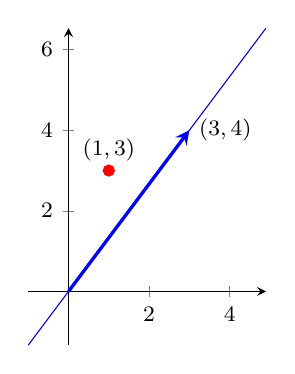
\begin{tikzpicture}
  \begin{axis}[small,font=\footnotesize
  ,axis equal image,axis lines=middle,samples=2 ,domain=-1:4.9]
  \addplot[blue,no marks]{4/3*x};
  \addplot[blue,very thick,quiver={u=3,v=4},-stealth]coordinates {(0,0)};
  \node[right] at (axis cs:3,4) {$(3,4)$};
  \addplot[red,mark=*] coordinates {(1,3)};
  \node[above] at (axis cs:1,3) {$(1,3)$};
  \end{axis}
\end{tikzpicture}}
\begin{activity}[\temp]
Consider the inconsistent equations \(3x=1\) and \(4x=3\) formed as the system (illustrated to the right)
\begin{equation*}
\begin{bmatrix} 3\\4 \end{bmatrix}x=\begin{bmatrix} 1\\3 \end{bmatrix},
\quad\text{and given }
\begin{bmatrix} 3\\4 \end{bmatrix}
=\begin{bmatrix} \frac35&\frac45\\\frac45&-\frac35 \end{bmatrix}
\begin{bmatrix} 5\\0 \end{bmatrix}
\tr{\begin{bmatrix} 1 \end{bmatrix}}
\end{equation*}
is an \svd\ \idx{factorization} of the \(2\times 1\) matrix.
Following the procedure of the previous \cref{eg:fourwts}, what is the `best' \idx{approximate solution} to these inconsistent equations?
\actposs[4]{\(x=3/5\)}{\(x=1/3\)}{\(x=4/7\)}{\(x=3/4\)}
\end{activity}
\endgroup



\begin{wrapfigure}r{0pt}
\qview{58}{63}{\begin{tikzpicture} 
\begin{axis}[small,font=\footnotesize,axis equal image,view={\q}{35}
  ,zmin=-2,zmax=2]
\addplot3[surf,domain=-1.5:1.5,opacity=0.5,samples=9] {y-x};
    \addplot3[quiver={u=1,v=1,w=0},blue,-stealth] 
    coordinates {(0,0,0)};
    \addplot3[quiver={u=-1,v=0,w=1},blue,-stealth] 
    coordinates {(0,0,0)};
    \addplot3[quiver={u=0,v=-1,w=-1},blue,-stealth] 
    coordinates {(0,0,0)};
    \addplot3[quiver={u=1,v=2,w=1},red,thick,-stealth] 
    coordinates {(0,0,0)};
    \node[] at (axis cs:1,2,1.5) {$\bv$};
\end{axis}
\end{tikzpicture}}
\end{wrapfigure}
\begin{example} \label{eg:rstp3}
Recall the \idx{table tennis} \idx{player rating} \cref{eg:rstp2}.
There we found that we could not solve the equations to find some ratings because the equations were \idx{inconsistent}.
In our new terminology of the previous \cref{sec:sbd}, the right-hand side vector~\bv\ is not in the \idx{column space} of the matrix~\(A\) (\cref{def:colsp}): 
the stereo picture to the right illustrates the 2D column space spanned by the three columns of~\(A\) and that the vector~\bv, of the results, lies outside the \text{column space.}

Now reconsider Step~3 in \cref{eg:rstp2}.
\begin{enumerate} \addtocounter{enumi}2
\item We need to interpret and `solve' \(S\yv=\zv\) which here is
\begin{equation*}
\begin{bmatrix} 1.7321&0&0
\\0&1.7321&0
\\0&0&0 \end{bmatrix}\yv=\begin{bmatrix} 
   -2.0412\\-2.1213\\0.5774
\end{bmatrix}.
\end{equation*}
The third line of this system says \(0y_3=0.5774\) which is impossible for any~\(y_3\): we cannot have zero on the left-hand side equalling \(0.5774\) on the right-hand side.
Instead of seeking an \emph{exact} solution, ask what is the \emph{\idx{smallest change}} we can make to~\(\zv=(-2.0412, -2.1213, 0.5774)\)\ so that we can report a solution, albeit to a slightly different problem?
Answer: we \emph{must} change the last component of~\zv\ to zero. 
Moreover, any change to the first two components is not needed, would make the change bigger than necessary, and so we do not change the first two components.
Hence we find an \idx{approximate solution} to the \idx{player rating}s via solving
\begin{equation*}
\begin{bmatrix} 1.7321&0&0
\\0&1.7321&0
\\0&0&0 \end{bmatrix}\yv=\begin{bmatrix} 
   -2.0412\\-2.1213\\0
\end{bmatrix}.
\end{equation*}
Here, via \verb|y=z(1:2)./diag(S(1:2,1:2))|, a general solution is that vector \(\yv=(-1.1785,-1.2247,y_3)\).
Varying the \idx{free variable}~\(y_3\) gives equally good approximate solutions.

\item Lastly, solve \(\tr V\xv=\yv\)\,, via computing \verb|x=V(:,1:2)*y|, to determine
\begin{eqnarray*}
\xv=V\yv&=&
\begin{bmatrix} 0.0000 & -0.8165 & 0.5774
\\ -0.7071 & 0.4082 & 0.5774
\\  0.7071 & 0.4082 & 0.5774
 \end{bmatrix}\begin{bmatrix} -1.1785\\-1.2247\\y_3 \end{bmatrix}
\\&=&\begin{bmatrix} 1\\\frac13\\-\frac43 \end{bmatrix}
+\frac{y_3}{\sqrt3}\begin{bmatrix} 1\\1\\1 \end{bmatrix}.
\end{eqnarray*}
\end{enumerate}
As before, it is only the relative ratings that are important so we  choose any particular (approximate) solution by setting~\(y_3\) to anything we like, such as zero.
The predicted ratings are then \(\xv=(1,\frac13,-\frac43)\) for Anne, Bob and Chris, respectively.
\end{example}

The reliability and likely error of such \idx{approximate solution}s are the province of Statistics courses.
We focus on the geometry and linear algebra of obtaining such a `best' approximate solution.



\begin{procedure}[\bfidx{approximate solution}]\label{pro:appsol}
    Obtain the so-called `\idx{least square}' approximate solution(s) of \idx{inconsistent} equations $A\xv=\bv$ using an \svd\ and via intermediate unknowns:
    \begin{enumerate}[ref=\ref{pro:appsol}(\alph*)]
    \item\label[step]{as:a0} factorize \(A=\usv\) and set \(r=\rank A\) (remembering that relatively small \idx{singular value}s are effectively zero);
        \item\label[step]{as:a1} solve \(U\zv=\bv\) by $\zv=\tr U\bv$;
    
        \item\label[step]{as:a2} disregard the inconsistent equations for \(i=r+1,\ldots,m\) as errors, set $y_i=z_i/\sigma_i$ for $i=1,\ldots,r$  (as these $\sigma_i> 0$), and otherwise $y_i$~is free for $i=r+1,\ldots,n$\,; 
    
        \item\label[step]{as:a4} solve \(\tr V\xv=\yv\) to obtain a general approximate solution as $\xv=V\yv$.
    \end{enumerate}
\end{procedure}




\begin{reduce}
\begin{example} \label{eg:twotcm} % adapted from Chong 2008, p.215
You are given the choice of two different types of concrete mix.
One type contains 40\%~cement, 40\%~gravel, and 20\%~sand; whereas the other type contains 20\%~cement, 10\%~gravel, and 70\%~sand.
How many kilograms of each type should you mix together to obtain a concrete mix as close as possible to \(3\)\,kg of cement, \(2\)\,kg of gravel, and \(4\)\,kg \text{of sand.}
\begin{solution} 
Let variables~\(x_1\) and~\(x_2\) be the as yet unknown amounts, in~kg, of each type of concrete mix. 
Then for the cement component we want \(0.4x_1+0.2x_2=3\), whereas for the gravel component we want \(0.4x_1+0.1x_2=2\), and for the sand component \(0.2x_1+0.7x_2=4\)\,.
These form the matrix-vector system \(A\xv=\bv\) for matrix and vector
\begin{equation*}
A=\begin{bmatrix} 0.4&0.2\\0.4&0.1\\0.2&0.7 \end{bmatrix},
\quad \bv=\begin{bmatrix} 3\\2\\4 \end{bmatrix}.
\end{equation*}
Apply \cref{pro:appsol}.
\begin{enumerate}
\item Enter the matrix~\(A\) and vector~\bv\ into \script\ with
\setbox\ajrqrbox\hbox{\qrcode{% round robin tournament
A=[0.4 0.2; 0.4 0.1; 0.2 0.7]
b=[3;2;4]
[U,S,V]=svd(A)
z=U'*b
y=z(1:2)./diag(S)
x=V*y
}}%
\marginajrbox%
\begin{verbatim}
A=[0.4 0.2; 0.4 0.1; 0.2 0.7]
b=[3;2;4]
\end{verbatim}
Then factorize matrix \(A=\usv\) with \verb|[U,S,V]=svd(A)|\,:
\begin{verbatim}
U =
  -0.4638  -0.5018  -0.7302
  -0.3681  -0.6405   0.6740
  -0.8058   0.5814   0.1123
S =
   0.8515        0
        0   0.4182
        0        0
V =
  -0.5800  -0.8146
  -0.8146   0.5800
\end{verbatim}
The system of equations \(A\xv=\bv\) for the mix becomes
\begin{equation*}
U\underbrace{S\overbrace{\tr V\xv}^{=\yv}}_{=\zv}
=\bv.
\end{equation*}
\item Solve \(U\zv=\bv\) by  \(\zv=\tr U\bv\) via computing \verb|z=U'*b| to get
\begin{verbatim}
z =
  -5.3510
  -0.4608
  -0.3932
\end{verbatim}

\item Now solve \(S\yv=\zv\).
But the last (third) row of the diagonal matrix~\(S\) is zero, whereas the last component of~\zv\ is nonzero: hence there is no exact solution. 
Instead we approximate by setting the last component of \zv\ to zero.
This approximation is the \emph{\idx{smallest change}} we can make to the required mix that \text{is possible.}

That is, since \(\rank A=2\) from the two nonzero singular values, so we approximately solve the system in \script\ by \verb|y=z(1:2)./diag(S)| (there are no free variables here):
\begin{verbatim}
y =
  -6.284
  -1.102
\end{verbatim}

\item Lastly solve \(\tr V\xv=\yv\) as \(\xv=V\yv\) by computing \verb|x=V*y|\,:
\begin{verbatim}
x =
   4.543
   4.479
\end{verbatim}
\end{enumerate}
Then interpret: from this solution \(\xv\approx(4.5,4.5)\) we need to mix close to 4.5\,kg of both the types of concrete to get as close as possible to the desired mix.
Multiplication, \(A\xv\) or~\verb|A*x|, tells us that the resultant mix is about \(2.7\)\,kg cement, \(2.3\)\,kg gravel, and \(4.0\)\,kg \text{of sand.}

Compute \verb|x=A\b| and find it directly gives exactly the same answer: \cref{sec:csap} discusses why~\verb|A\b| gives exactly the same `best' approximate solution. 
\end{solution}
\end{example}
\end{reduce}






\begin{example}[round robin tournament] \label{eg:roundrobin1}
Consider four players (or teams) that play in a round robin sporting event: Anne, Bob, Chris and Dee.
\cref{tbl:roundrobin1} summarizes the results of the six games played.
\begin{table}
\caption{the results of six games played in a round robin: the scores are games\slash goals\slash points scored by each when playing the others.  For example, Dee beat Anne 3~to~1.}
\label{tbl:roundrobin1}
\begin{center}
\begin{tabular}{l|cccc} \hline
&Anne& Bob& Chris& Dee\\ \hline
Anne & - & 3 & 3 & 1 \\
Bob & 2 & - & 2 & 4 \\
Chris & 0 & 1 & - & 2 \\
Dee & 3 & 0 & 3 & - \\ \hline
\end{tabular}
\end{center}
\end{table}%
From these results estimate the relative \idx{player rating}s of the four players.
As in many real-life situations, the information appears contradictory such as Anne beats Bob, who beats Dee, who in turn beats Anne.
Assume that the rating~\(x_i\) of player~\(i\) is to reflect, as best we can, the difference in scores upon playing player~\(j\):  that is, pose the difference in ratings, \(x_i-x_j\)\,, should equal the difference in the scores when \text{they play.}
\begin{solution} 
The first stage is to model the results by idealised mathematical equations.
From \cref{tbl:roundrobin1} six games were played with the following scores.  
Each game then generates the shown ideal equation for the difference between \text{two ratings.}
\begin{itemize}
\item Anne beats Bob 3-2, so \(x_1-x_2=3-2=1\)\,.
\item Anne beats Chris 3-0, so \(x_1-x_3=3-0=3\)\,.
\item Bob beats Chris 2-1, so \(x_2-x_3=2-1=1\)\,.
\item Anne is beaten by Dee 1-3, so \(x_1-x_4=1-3=-2\)\,.
\item Bob beats Dee 4-0, so \(x_2-x_4=4-0=4\)\,.
\item Chris is beaten by Dee 2-3, so \(x_3-x_4=2-3=-1\)\,.
\end{itemize}
These six equations form the linear system \(A\xv=\bv\) where
\begin{equation*}
A=\begin{bmatrix}    1 & -1 & 0 & 0
\\ 1 & 0 & -1 & 0
\\ 0 & 1 & -1 & 0
\\ 1 & 0 & 0 & -1
\\ 0 & 1 & 0 & -1
\\ 0 & 0 & 1 & -1
 \end{bmatrix},\quad
 \bv=\begin{bmatrix} 1\\ 3\\ 1\\ -2\\ 4\\ -1 \end{bmatrix}.
\end{equation*}
We cannot satisfy all these equations exactly, so we have to accept an approximate solution that estimates the ratings as best we can.
The second stage uses an \svd\ and \cref{pro:appsol} to `best' solve the equations.
\begin{enumerate}
\item Enter the matrix~\(A\) and vector~\bv\ into \script\ with
\setbox\ajrqrbox\hbox{\qrcode{% round robin tournament
A=[1  -1   0   0
   1   0  -1   0
   0   1  -1   0
   1   0   0  -1
   0   1   0  -1
   0   0   1  -1 ]
b=[1;3;1;-2;4;-1]
[U,S,V]=svd(A)
}}%
\marginajrbox%
\begin{verbatim}
A=[1  -1   0   0
   1   0  -1   0
   0   1  -1   0
   1   0   0  -1
   0   1   0  -1
   0   0   1  -1 ]
b=[1;3;1;-2;4;-1]
\end{verbatim}
Then factorize  matrix \(A=\usv\) with \verb|[U,S,V]=svd(A)| \twodp:
\begin{verbatim}
U =
  0.31 -0.26 -0.58 -0.26  0.64 -0.15
  0.07  0.40 -0.58  0.06 -0.49 -0.51
 -0.24  0.67  0.00 -0.64  0.19  0.24
 -0.38 -0.14 -0.58  0.21 -0.15  0.66
 -0.70  0.13  0.00  0.37  0.45 -0.40
 -0.46 -0.54 -0.00 -0.58 -0.30 -0.26
S =
  2.00     0     0     0
     0  2.00     0     0
     0     0  2.00     0
     0     0     0  0.00
     0     0     0     0
     0     0     0     0
V =
  0.00  0.00 -0.87 -0.50
 -0.62  0.53  0.29 -0.50
 -0.14 -0.80  0.29 -0.50
  0.77  0.28  0.29 -0.50
\end{verbatim}
Although the first three columns of \verb|U| and~\verb|V| may be different for you (because the first three singular values are all the same),  the eventual solution is the same.
The system of equations \(A\xv=\bv\) for the ratings becomes
\begin{equation*}
U\underbrace{S\overbrace{\tr V\xv}^{=\yv}}_{=\zv}
=\bv.
\end{equation*}

\item Solve \(U\zv=\bv\) by  \(\zv=\tr U\bv\) via computing \verb|z=U'*b| to get the \(\RR^6\) vector
\begin{verbatim}
z =
  -1.27
   2.92
  -1.15
   0.93
   1.76
  -4.07
\end{verbatim}

\item Now solve \(S\yv=\zv\).
But the last three rows of the diagonal matrix~\(S\) are zero, whereas the last three components of~\zv\ are nonzero: hence there is no exact solution. 
Instead we approximate by setting the last three components of \zv\ to zero.
This approximation is the \emph{\idx{smallest change}} we can make to the data of the game results that makes the \text{results consistent.}

That is, since \(\rank A=3\) from the three nonzero singular values, so we approximately solve the system in \script\ by \verb|y=z(1:3)./diag(S(1:3,1:3))|\,:
\begin{verbatim}
y =
  -0.63
   1.46
  -0.58
\end{verbatim}
The fourth component~\(y_4\) is arbitrary.

\item Lastly, solve \(\tr V\xv=\yv\) as \(\xv=V\yv\)\,. 
Obtain a particular solution in \script\ by computing \verb|x=V(:,1:3)*y|\,:
\begin{verbatim}
x =
   0.50
   1.00
  -1.25
  -0.25
\end{verbatim}
Add an arbitrary multiple of the fourth column of~\verb|V| to get a general solution
\begin{equation*}
\xv=\begin{bmatrix} \frac12\\1\\-\frac54\\-\frac14 \end{bmatrix}
+y_4\begin{bmatrix} -\frac12\\ -\frac12\\ -\frac12\\ -\frac12 \end{bmatrix}.
\end{equation*}
\end{enumerate}
The final stage is to interpret the solution for the application.
In this application the absolute ratings are not important, so we ignore~\(y_4\) (consider it zero).  
From the game results of \cref{tbl:roundrobin1} this analysis indicates the players' rankings are, in decreasing order, Bob, Anne, Dee, \text{and Chris.}
\end{solution}
\end{example}



\begin{table}
\begin{minipage}{\linewidth}
\hrulefill\\
Be aware of \index{Arrow, Kenneth}Kenneth Arrow's \idx{Impossibility Theorem} \cite[]{Arrow50}---one of the great theorems of the 20th~century: \emph{all 1D ranking systems are flawed!}  
\idx{Wikipedia}\footnote{\protect\url{https://en.wikipedia.org/wiki/Arrow\%27s\_impossibility\_theorem}}
 (2014) described the theorem this way (in the context of voting systems): that among 
\begin{quote}
three or more distinct alternatives (options), no rank order voting system can convert the ranked preferences of individuals into a community-wide (complete and transitive) ranking while also meeting [four sensible] criteria \ldots\ called unrestricted domain, non-dictatorship, Pareto efficiency, and independence of irrelevant alternatives.
\end{quote}
In rating sport players\slash teams:
\begin{itemize}
\item the ``distinct alternatives'' are the players\slash teams;
\item  the ``ranked preferences of individuals'' are the individual results of each game played; and 
\item the ``community-wide ranking'' is the assumption that we can rate each player\slash team by a one-dimensional numerical rating.
\end{itemize}
Arrow's theorem assures us that every such scheme must violate at least one of four sensible criteria.
Every ranking scheme is thus open to criticism. 
But every alternative scheme would also be open to criticism by also violating at least one of \text{the criteria.}
\end{minipage}
\end{table}


When rating players or teams based upon results, be clear the purpose.  
For example, is the purpose to summarize past performance? or to predict future contests?  
% should we remove these question marks??
If the latter, then my limited experience suggests that one should fit the win-loss record instead of the scores.
Explore the alternatives for your \text{favourite sport.}




\begin{comment}
Further applications include least square regression  \larsvii{p.92--4*} \holti{p.399--401}, least square approximations, and Fourier series \larsvii{p.275--281}.
\end{comment}



\begin{activity}
Listed below are four \idx{approximate solution}s to the system \(A\xv=\bv\)\,,
\begin{equation*}
\begin{bmatrix} 5&3\\3&-1\\1&1 \end{bmatrix}\begin{bmatrix} x\\y \end{bmatrix}=\begin{bmatrix} 9\\2\\10 \end{bmatrix}.
\end{equation*}
Setting vector \(\bv'=A\xv\) for each, which one minimizes the \idx{distance} between the original right-hand side \(\bv=(9,2,10)\) and the approximate~\(\bv'\)?
\actposs[4]{\(\xv=\begin{bmatrix} 1\\2 \end{bmatrix}\)}
{\(\xv=\begin{bmatrix} 1\\1 \end{bmatrix}\)}
{\(\xv=\begin{bmatrix} 2\\1 \end{bmatrix}\)}
{\(\xv=\begin{bmatrix} 2\\2 \end{bmatrix}\)}
\end{activity}



\begin{theorem}[\bfidx{smallest change}] \label{thm:appsol} 
All \idx{approximate solution}s obtained by \cref{pro:appsol} solve the linear \idx{system} \(A\xv=\bv'\) for the unique \idx{consistent} right-hand side vector~\(\bv'\) 
that minimizes the \idx{distance}~\(|\bv'-\bv|\).
\end{theorem}
(The dash on~\(\bv'\)\ is to suggest an approximation to~\bv.)
\begin{proof} 
Find an \svd\ \(A=\usv\) of \(m\times n\) matrix~\(A\).
Then \cref{pro:appsol} computes \(\zv=\tr U\bv\in\RR^m\), that is, \(\bv=U\zv\) as \(U\)~is orthogonal.
For any \(\bv'\in\RR^m\) let \(\zv'=\tr U\bv'\in\RR^m\), that is, \(\bv'=U\zv'\).
Then \(|\bv'-\bv|=|U\zv'-U\zv|=|U(\zv'-\zv)|=|\zv'-\zv|\) as multiplication by orthogonal~\(U\) preserves distances (\cref{thm:orthog}).
Thus minimizing~\(|\bv'-\bv|\) is equivalent to minimizing~\(|\zv'-\zv|\).
\cref{pro:appsol} seeks to solve the diagonal system \(S\yv=\zv\) for \(\yv\in\RR^n\). 
That is, for a matrix of \(\rank A=r\)
\begin{equation*}
\begin{bmatrix} \begin{matrix} \sigma_1&\cdots&0\\
\vdots&\ddots&\vdots\\
0&\cdots&\sigma_r \end{matrix} & 
O_{r\times (n-r)}\\\,\\
O_{(m-r)\times r}&O_{(m-r)\times (n-r)}
\\\,\end{bmatrix}\yv
=\begin{bmatrix} z_1\\\vdots\\z_r\\z_{r+1}\\\vdots\\z_m \end{bmatrix}.
\end{equation*}
\cref{pro:appsol} approximately solves this inconsistent system by adjusting the right-hand side to \(\zv'=(z_1,\ldots,z_r,0,\ldots,0)\in\RR^m\).
This change makes \(|\zv-\zv'|\) as small as possible because we \emph{must} zero the last \((m-r)\)~components of~\zv\ in order to obtain a consistent set of equations, and because any adjustment to the first \(r\)~components of~\zv\ would only increase~\(|\zv-\zv'|\).
Further, it is the only change to~\zv\ that does so, so \(\zv'\)~is the unique minimizer.
Hence the solution computed by \cref{pro:appsol} solves the consistent system \(A\xv=\bv'\) (with the unique \(\bv'=U\zv'\)) such that \(|\bv-\bv'|\) \text{is minimized.}
\end{proof}




\begin{example}[\idx{life expectancy}] \label{eg:lifeExpectancy}
\begin{table}
\caption{life expectancy in years of (white) \idx{female}s and males born in the given years  [\url{http://www.infoplease.com/ipa/A0005140.html}, 2014].  Used by \cref{eg:lifeExpectancy}.}
\label{tbl:lifeExpectancy}
\begin{equation*}
\begin{array}{lrrrrrrrr} \hline
\text{year}&1951&1961&1971&1981&1991&2001&2011\\\hline
\text{female}&72.0&74.2&75.5&78.2&79.6&80.2&81.1\\
\text{male}&66.3&67.5&67.9&70.8&72.9&75.0&76.3\\\hline
\end{array}
\end{equation*}
\end{table}
\begin{figure}
\centering
%\includegraphics[width=\linewidth]{lifeExpectancy}
\input{Matrices/lifeExpectancy.ltx}
\caption{the life expectancies in years of females and males born in the given years (\cref{tbl:lifeExpectancy}).  
Also plotted is the \idx{best straight line} fit to the female data obtained by \cref{eg:lifeExpectancy}.}
\label{fig:lifeExpectancy}
\end{figure}
\cref{tbl:lifeExpectancy} lists life expectancies of people born in a given year; \cref{fig:lifeExpectancy} plots the data points.
Over the decades the life expectancies have increased.
Let's quantify the overall trend to be able to draw, as in 
\cref{fig:lifeExpectancy}, the \idx{best straight line} to the 
female \idx{life expectancy}.
Solve the approximation problem with an \svd\ and confirm it gives the same solution as~\verb|A\b| in \script.
\begin{solution} 
Start by posing a mathematical model: let's suppose that the life expectancy~\(\ell\) is a straight line function of year of birth: \(\ell=x_1+x_2t\) where we need to find the coefficients \(x_1\) and~\(x_2\), and where \(t\)~counts the number of decades since~1951, the start of the data.
\cref{tbl:lifeExpectancy} then gives seven ideal equations to solve for \(x_1\) and~\(x_2\):
\begin{eqnarray*}
(1951)&&x_1+0x_2=72.0\,,
\\(1961)&&x_1+1x_2=74.2\,,
\\(1971)&&x_1+2x_2=75.5\,,
\\(1981)&&x_1+3x_2=78.2\,,
\\(1991)&&x_1+4x_2=79.6\,,
\\(2001)&&x_1+5x_2=80.2\,,
\\(2011)&&x_1+6x_2=81.1\,.
\end{eqnarray*}
Form these into the matrix-vector system \(A\xv=\bv\) where
\begin{equation*}
A= \begin{bmatrix} 1&0\\1&1\\1&2\\1&3\\1&4\\1&5\\1&6 \end{bmatrix},
\quad \bv=\begin{bmatrix}72.0\\74.2\\75.5\\78.2\\79.6\\80.2\\81.1\end{bmatrix}.
\end{equation*}
\cref{pro:appsol} then determines a best approximate solution.
\begin{enumerate}
\item Enter the matrix~\(A\) and vector~\bv\ into \script, and compute an \svd\ of \(A=\usv\) via \verb|[U,S,V]=svd(A)| \twodp:
\setbox\ajrqrbox\hbox{\qrcode{% life expectancy
A=[ones(7,1) (0:6)' ]
b=[72.0;74.2;75.5;78.2;79.6;80.2;81.1]
[U,S,V]=svd(A)
}}%
\marginajrbox%
\begin{verbatim}
U =
  0.02  0.68 -0.38 -0.35 -0.32 -0.30 -0.27
  0.12  0.52 -0.14  0.06  0.26  0.45  0.65
  0.22  0.36  0.89 -0.09 -0.08 -0.07 -0.05
  0.32  0.20 -0.10  0.88 -0.13 -0.15 -0.16
  0.42  0.04 -0.10 -0.14  0.81 -0.23 -0.28
  0.52 -0.12 -0.09 -0.16 -0.24  0.69 -0.39
  0.62 -0.28 -0.09 -0.19 -0.29 -0.40  0.50
S =
  9.80     0
     0  1.43
     0     0
     0     0
     0     0
     0     0
     0     0
V =
  0.23  0.97
  0.97 -0.23
\end{verbatim}
\item Solve \(U\zv=\bv\) to give this first intermediary \(\zv=\tr U\bv\) via the command \verb|z=U'*b|\,:
\begin{verbatim}
z =
   178.19
   100.48
    -0.05
     1.14
     1.02
     0.10
    -0.52
\end{verbatim}

\item Now solve approximately \(S\yv=\zv\)\,. 
From the two nonzero singular values in~\(S\) the matrix~\(A\) has rank~\(2\).
So the approximation is to discard\slash zero (as `errors') all but the first two elements of~\zv\ and find the best approximate~\yv\ via \verb|y=z(1:2)./diag(S(1:2,1:2))|\,:
\begin{verbatim}
y =
   18.19
   70.31
\end{verbatim}

\item Solve \(\tr V\xv=\yv\) by \(\xv=V\yv\) via \verb|x=V*y|\,:
\begin{verbatim}
x =
   72.61
    1.55
\end{verbatim}
\end{enumerate}
Compute \verb|x=A\b| to find it gives exactly the same answer: \cref{sec:csap} discusses why~\verb|A\b| gives exactly the same `best' approximate solution. 

Lastly, interpret the answer.
The approximation gives \(x_1=72.61\) and \(x_2=1.55\) \twodp.  
Since the ideal model was life expectancy \(\ell=x_1+x_2t\) we  determine a `best' approximate model is \(\ell\approx72.61+1.55\,t\) years where \(t\)~is the number of decades since 1951: this is the straight line drawn in \cref{fig:lifeExpectancy}.
That is, females tend to live an extra 1.55~years for every decade born after 1951.
For example, for females born in 2021, some seven decades after 1951, this model predicts a life expectancy of \(\ell\approx72.61+1.55\times7=83.46\)~years.
\end{solution}
\end{example}



\begin{activity}\label{eg:flowmeter}
In calibrating a vortex flowmeter the following flow rates were obtained for various applied voltages.
\begin{equation*}
\begin{array}{lrrrr}\hline
\text{voltage (V)}&1.18&1.85&2.43&2.81\\
\text{flow rate (litre/s)}&0.18&0.57&0.93&1.27\\\hline
\end{array}
\end{equation*}
Letting \(v_i\) be the voltages and \(f_i\)~the flow rates, which of the following is a reasonable model to seek? (for coefficients~\(x_1,x_2,x_3\))
\actposs{\(f_i=x_1+x_2v_i\)}
{\(f_i=x_1\)}
{\(v_i=x_1+x_2f_i\)}
{\(v_i=x_1+x_2f_i+x_3f_i^2\)}
\end{activity}



\begin{table}
\hrule
\begin{minipage}{\linewidth}
\paragraph{Power laws and the log-log plot}
Hundreds of power-laws have been identified in engineering, physics, biology and the social sciences.
These laws are typically detected via \idx{log-log plot}s.
A log-log plot is a two-dimensional graph of the numerical data that uses a logarithmic scale on both the horizontal and vertical axes, as in \cref{fig:orbitalPeriods}.
Then curvaceous relationships of the form $y=cx^a$ between the vertical variable,~$y$, and the horizontal variable,~$x$, appear as straight lines on a \idx{log-log plot}.
For example, below-left is plotted the three curves $y\propto x^2$,  $y\propto x^3$, and  $y\propto x^4$.
It is hard to tell which \text{is which.}
\begin{center} 
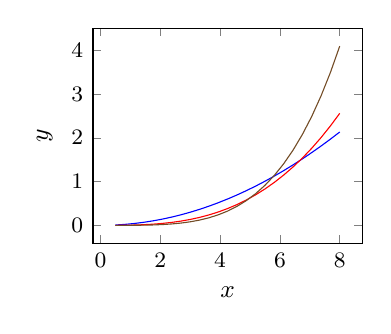
\begin{tikzpicture}
\begin{axis}[footnotesize,domain=0.5:8,no marks,xlabel={$x$},ylabel={$y$}]
\addplot+{x^2/30};
\addplot+{x^3/200};
\addplot+{x^4/1000};
\end{axis} 
\end{tikzpicture} \hfil
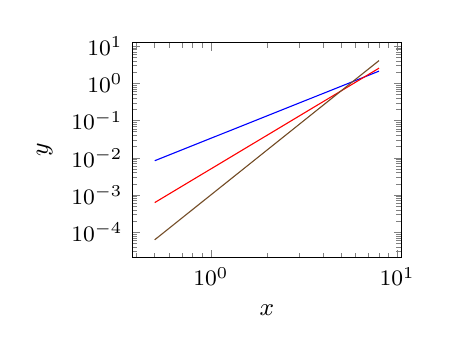
\begin{tikzpicture}
\begin{loglogaxis}[footnotesize,domain=0.5:8,no marks,xlabel={$x$},ylabel={$y$}]
\addplot+{x^2/30};
\addplot+{x^3/200};
\addplot+{x^4/1000};
\end{loglogaxis} 
\end{tikzpicture} 
\end{center}
However, plot the same curves on the above-right \idx{log-log plot} and it  distinguishes the curves as different straight lines: the steepest line is the curve with the largest exponent, $y\propto x^4$, whereas the least-steep line is the curve with the smallest exponent, $y\propto x^2$.

%\begin{verbatim}
%x=10.^(cumsum(1+rand(3,1))/5), y=x.^2.618/5
%x=round(x*10)/10, y=round(y*10)/10
%A=[log10(x) ones(3,1)]
%ab=A\log10(y)
%octave:35> A=[log10(x) ones(3,1)]
%A =
%   0.2553   1.0000
%   0.5185   1.0000
%   0.8261   1.0000
%octave:36> ab=A\log10(y)
%ab =
%   2.6437
%  -0.7162
%\end{verbatim}
For example, suppose you make three measurements that at $x=1.8,3.3,6.7$ the value of $y=0.9,4.6,29.1$, respectively.  
The graph below-left show the three data points~$(x,y)$.  
Find the power law curve $y=cx^a$ that explains these points.
\begin{center} 
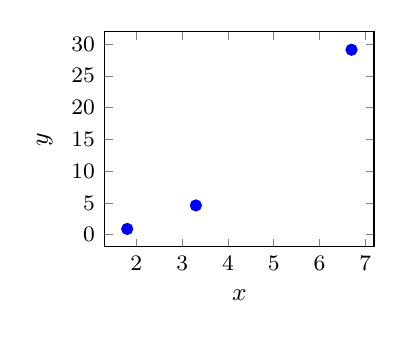
\begin{tikzpicture}
\begin{axis}[footnotesize,domain=0.5:8,xlabel={$x$},ylabel={$y$}]
\addplot+[only marks] coordinates {(1.8,0.9)(3.3,4.6)(6.7,29.1)};
\end{axis} 
\end{tikzpicture} \hfil
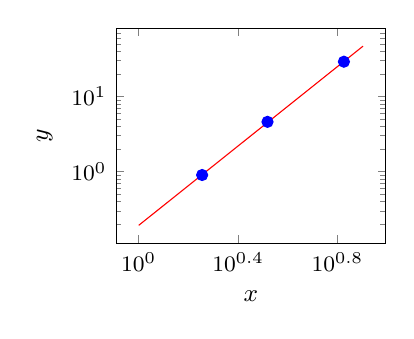
\begin{tikzpicture}
\begin{loglogaxis}[footnotesize,xlabel={$x$},ylabel={$y$},xtick={1,2.512,6.310}]
\addplot+[only marks] coordinates {(1.8,0.9)(3.3,4.6)(6.7,29.1)};
\addplot+[no marks] coordinates {(1,0.1922)(8,46.91)};
\end{loglogaxis} 
\end{tikzpicture} 
\end{center}
Take the \idx{logarithm} (to any base so let's choose base~$10$) of both sides of $y=cx^a$ to get $\log_{10} y=(\log_{10} c)+a(\log_{10} x)$, equivalently, $(\log_{10} y)=a(\log_{10} x)+b$ for constant $b=\log_{10} c$\,.
That is, there is a straight line relationship between $(\log_{10} y)$ and $(\log_{10} x)$, as illustrated above-right.
Here $\log_{10}x=0.26,0.52,0.83$ and $\log_{10}y=-0.04,0.66,1.46$, respectively \twodp.
Using the end points to estimate the slope gives $a=2.63$, the exponent in the power law.
Then the constant $b=-0.04-2.63\cdot0.26=-0.72$ so the coefficient $c=10^b=0.19$\,.
That is, via the \idx{log-log plot}, the power law $y=0.19\cdot 2.63^x$ explains the data.
Such log-log plots are not only used in \cref{eg:orbitalPeriods}, they are endemic in science \text{and engineering.}
\end{minipage}
\hrule
\end{table}




\begin{example}[planetary \idx{orbital period}s] \label{eg:orbitalPeriods}
\begin{table}
\caption{orbital periods for the eight \idx{planets} of the \idx{solar system}: the periods are in (Earth) days; the distance is the length of the semi-major axis of the orbits (\idx{Wikipedia}, 2014).
Used by \cref{eg:orbitalPeriods}.}
\label{tbl:orbitalPeriods}
% the original source of this data is not cited by Wikipedia
{\footnotesize[\protect\url{https://en.wikipedia.org/wiki/Orbital\_period}]}
\begin{equation*}
\begin{array}{p{12ex}rr} \hline
planet&\text{distance}&\text{period}\\
&\text{(Gigametres)}&\text{(days)}\\\hline
Mercury& 57.91 & 87.97 \\
Venus& 108.21 & 224.70 \\
Earth& 149.60& 365.26\\
Mars& 227.94& 686.97\\
Jupiter& 778.55& 4332.59\\
Saturn& 1433.45& 10759.22\\
Uranus& 2870.67& 30687.15\\
Neptune& 4498.54& 60190.03\\\hline
\end{array}
\end{equation*}
\end{table}%
\begin{figure}
\centering
\input{Matrices/orbitalPeriods.ltx}
\caption{the planetary periods as a function of the distance from the data of \cref{tbl:orbitalPeriods}: the graph is a \idx{log-log plot} to show the excellent power law.  
Also plotted is the power law fit computed by \cref{eg:orbitalPeriods}.}
\label{fig:orbitalPeriods}
\end{figure}%
\cref{tbl:orbitalPeriods} lists each \idx{orbital period} of the \idx{planets} of the \idx{solar system}; \cref{fig:orbitalPeriods} plots the data points as a function of the distance of the planets from the sun.
Let's infer \idx{Kepler's law} that the period grows as the distance to the power~\(3/2\): shown by the \idx{best straight line} fit in \cref{fig:orbitalPeriods}.
Use the data for the planets from Mercury to Uranus to infer the law with an \svd, confirm it gives the same solution as~\verb|A\b| in \script, and use the fit to predict Neptune's period from \text{its distance.}
\begin{solution} 
Start by posing a mathematical model: Kepler's law is a power law that the \(i\)th~period \(p_i=c_1d_i^{c_2}\) for some unknown coefficient~\(c_1\) and exponent~\(c_2\).  
Take logarithms (to any base so let's use base~\(10\)) and seek that 
\(\log_{10}p_i=\log_{10} c_1+c_2\log_{10}d_i\)\,; that is, seek unknowns \(x_1\) and~\(x_2\) such that \(\log_{10}p_i=x_1+x_2\log_{10}d_i\)\,.
The first seven rows of \cref{tbl:orbitalPeriods} then gives seven ideal linear equations to solve for \(x_1\) and~\(x_2\):
\begin{eqnarray*}
&&x_1+\log_{10}57.91\,x_2=\log_{10}87.97\,, %&\implies&x_1+1.76x_2=1.94\,,
\\&&x_1+\log_{10}108.21\,x_2=\log_{10}224.70\,, %&\implies&x_1+2.03x_2=2.35\,,
\\&&x_1+\log_{10}149.60\,x_2=\log_{10}365.26\,, %&\implies&x_1+2.17x_2=2.56\,,
\\&&x_1+\log_{10}227.94\,x_2=\log_{10}686.97\,, %&\implies&x_1+2.36x_2=2.84\,,
\\&&x_1+\log_{10}778.55\,x_2=\log_{10}4332.59\,, %&\implies&x_1+2.89x_2=3.64\,,
\\&&x_1+\log_{10}1433.45\,x_2=\log_{10}10759.22\,, %&\implies&x_1+3.16x_2=4.03\,,
\\&&x_1+\log_{10}2870.67\,x_2=\log_{10}30687.15\,. %&\implies&x_1+3.46x_2=4.49\,.
\end{eqnarray*}
Form these into the matrix-vector system \(A\xv=\bv\)\,:
for simplicity recorded here to two decimal places albeit computed more accurately,
\begin{equation*}
A= \begin{bmatrix}   1&1.76\\
   1&2.03\\
   1&2.17\\
   1&2.36\\
   1&2.89\\
   1&3.16\\
   1&3.46
 \end{bmatrix},
\quad \bv=\begin{bmatrix}   1.94\\
   2.35\\
   2.56\\
   2.84\\
   3.64\\
   4.03\\
   4.49
\end{bmatrix}.
\end{equation*}

\cref{pro:appsol} then determines a best approximate solution.
\begin{enumerate}
\item Enter these matrices in \script\ by the commands, for example,
\setbox\ajrqrbox\hbox{\qrcode{% planetary orbit periods
d=[   57.91
     108.21
     149.60
     227.94
     778.55
    1433.45
    2870.67];
p=[ 87.97
   224.70
   365.26
   686.97
  4332.59
 10759.22
 30687.15];
A=[ones(7,1) log10(d)]
b=log10(p)
[U,S,V]=svd(A)
}}%
\marginajrbox%
\begin{verbatim}
d=[   57.91
     108.21
     149.60
     227.94
     778.55
    1433.45
    2870.67];
p=[ 87.97
   224.70
   365.26
   686.97
  4332.59
 10759.22
 30687.15];
A=[ones(7,1) log10(d)]
b=log10(p)
\end{verbatim}
since the \script\ function \index{log10()@\texttt{log10()}}\verb|log10()| computes the logarithm to base~\(10\) of each component in its argument (\cref{tbl:mtlbmops}).
Then compute an \svd\ of \(A=\usv\) via \verb|[U,S,V]=svd(A)| \twodp:
\begin{verbatim}
U =
 -0.27 -0.57 -0.39 -0.38 -0.34 -0.32 -0.30
 -0.31 -0.40 -0.21 -0.09  0.27  0.45  0.65
 -0.32 -0.31  0.88 -0.10 -0.06 -0.04 -0.02
 -0.35 -0.19 -0.11  0.90 -0.10 -0.09 -0.09
 -0.41  0.14 -0.08 -0.11  0.80 -0.25 -0.30
 -0.45  0.31 -0.06 -0.11 -0.26  0.67 -0.41
 -0.49  0.51 -0.04 -0.11 -0.31 -0.41  0.47
S =
  7.38     0
     0  0.55
     0     0
     0     0
     0     0
     0     0
     0     0
V =
 -0.35 -0.94
 -0.94  0.35
\end{verbatim}
\item Solve \(U\zv=\bv\) to give this first intermediary \(\zv=\tr U\bv\) via the command \verb|z=U'*b|\,:
\begin{verbatim}
z =
  -8.5507
   0.6514
   0.0002
   0.0004
   0.0005
  -0.0018
   0.0012
\end{verbatim}

\item Now solve approximately \(S\yv=\zv\)\,. 
From the two nonzero singular values in~\(S\) the matrix~\(A\) has rank two.
So the approximation is to discard\slash zero all but the first two elements of~\zv\ (as an error, here all small in value).
Then find the best approximate~\yv\ via the command \verb|y=z(1:2)./diag(S(1:2,1:2))|\,:
\begin{verbatim}
y =
  -1.1581
   1.1803
\end{verbatim}

\item Solve \(\tr V\xv=\yv\) by \(\xv=V\yv\) via \verb|x=V*y|\,:
\begin{verbatim}
x =
  -0.6980
   1.4991
\end{verbatim}
\end{enumerate}
Also check that computing \verb|x=A\b| gives exactly the same `best' approximate solution. 

Lastly, interpret the answer.
The approximation gives \(x_1=-0.6980\) and \(x_2=1.4991\)\,.  
Since the ideal model was the log of the period \(\log_{10}p=x_1+x_2\log_{10}d\) we determine a `best' approximate model is \(\log_{10}p\approx-0.6980+1.4991\log_{10}d\)\,. 
Raising ten to the power of both sides gives the power law that the period \(p\approx0.2005\,d^{1.4991}\)~days: this is the straight line drawn in \cref{fig:orbitalPeriods}.
The exponent~\(1.4991\) is within~\(0.1\)\% of the exponent~\(3/2\) that is \text{Kepler's law.}

For example, for Neptune with a semi-major axis distance of \(4498.542\)\,Gm, using the `best' model predicts Neptune's period\[10^{-0.6980+1.4991\log_{10}4498.542}=60019\text{ days.}\]
This prediction is pleasingly close to the observed period of \(60190\)~days.
\end{solution}
\end{example}





\begin{compute}
There are two separate important computational issues.
\begin{itemize}
\item Many books \idx{approximate solution}s of \(A\xv=\bv\) by solving the associated \idx{normal equation} \((\tr AA)\xv=(\tr A\bv)\).  
For \emph{theoretical purposes} this \idx{normal equation} is very useful.  
However, in practical computation avoid the normal equation because forming~\(\tr AA\), and then manipulating it, is both expensive and error enhancing (especially in large problems).
For example, \(\cond(\tr AA)=(\cond A)^2\) (\cref{ex:ctrAA}) so matrix~\(\tr AA\) typically has a much worse \idx{condition number} than matrix~\(A\) (\cref{pro:unisol}).
To paraphrase Cleve Molar: Almost anything you can do with~\(\tr AA\) can be done without it [via the \svd].


\item The last two examples observe that \verb|A\b| gives an answer that was identical to what the \svd\ procedure gives.
Thus \verb|A\b| can serve as a very useful short-cut to finding a best \idx{approximate solution}.
For non-square matrices with more rows than columns (more equations than variables), \verb|A\b| generally does this (without comment as \script\ assume you know what you are doing).
For other scenarios \verb|A\b| does something different, so \text{be wary.}
\end{itemize}
\end{compute}



\begin{comment}
\nakos{\S8.9} has some useful applications to USA NRL rating of quarterbacks---using data from \emph{The Sports Illustrated 19xx Sports Almanac}.
\end{comment}




\needspace{7\baselineskip}
\subsection{Compute the smallest appropriate solution}
\label{sec:csap}

\begin{quoted}{\index{Moler, Cleve}\parbox[t]{0.5\linewidth}{Cleve Moler, \emph{The world's simplest impossible problem} (1990)}}
I'm thinking of two numbers.  Their average is three.  What are the numbers?
\end{quoted}

\begin{comment}
Chapter~20 of the book by \cite{Higham1996} has some aspects of this section (including pseudo-inverse).
Matlab and Octave currently differ in that octave returns the smallest solution, but matlab returns a solution with at least \(m\)~nonzero elements??
\end{comment}

\paragraph{The \script\ operation \texttt{A$\backslash$b}}
\cref{eg:lifeExpectancy,eg:orbitalPeriods} observe that \verb|A\b|\index{A\slosh@\texttt{A\slosh}} gives an answer identical to the best \idx{approximate solution} given by the \svd\ \cref{pro:appsol}.
But there are just as many circumstances when \verb|A\b| is not `the approximate answer' that you want.
Beware.


\begin{example} 
Use \verb|x=A\b| to `solve' the problems of \cref{eg:fourwts,eg:rstp3,eg:roundrobin1}.
\begin{itemize}
\item With \script[2], observe the answer returned is the \emph{particular} solution determined by the \svd\ \cref{pro:appsol} (whether approximate or exact): 
respectively \(84.5\)\,kg; 
ratings \((1,\frac13,-\frac43)\); and 
ratings \((\frac12,1,-\frac54,-\frac14)\). %norm=1.70
\item With \script[1] (R2013b), the computed answers are often different: 
respectively \(84.5\)\,kg (the same); 
ratings \index{NaN@\texttt{NaN}}\index{Inf@\texttt{Inf}}\((\verb|NaN|,\verb|Inf|,\verb|Inf|)\) with a warning; 
and ratings \((\tfrac34,\tfrac54,-1,0)\) with a warning. %norm=1.77
\end{itemize}
How do we make sense of such differences in computed answers?
\end{example}

Recall that systems of linear equations may not have \idx{unique solution}s (as in the rating examples): what does~\verb|A\b|\index{A\slosh@\texttt{A\slosh}} compute when there are an infinite number of solutions?
\begin{itemize}
\item For systems of equations with the number of equations not equal to the number of variables, \(m\neq n\)\,, the \script[2] operation~\verb|A\b| computes for you the \emph{\idx{smallest solution}}
(that is, a solution that is of least \idx{magnitude}, smallest norm)
of all valid solutions (\cref{thm:smallsoln}): often `exact' when \(m<n\)\,, or approximate when \(m>n\) (\cref{thm:appsol}).  
Using~\verb|A\b| is the most efficient computationally, but using the \svd\ helps us understand what \text{it does.}

\item \script[1] (R2013b etc.) does something different with~\verb|A\b| in the case of fewer equations than variables, \(m<n\)\,. 
\script[1]'s different `answer' does reinforce that a choice of one solution among many is a subjective decision.
But \script[2]'s choice of the smallest valid solution is often \text{more appealing.}

\end{itemize}

\begin{theorem}[\bfidx{smallest solution}] \label{thm:smallsoln}
Obtain the {smallest solution}, whether exact or as an approximation, to a system of \idx{linear equation}s by invoking \cref{pro:gensol} or \cref{pro:appsol}, respectively, and then setting to \idx{zero} the \idx{free variable}s, that is, \(y_{r+1}=\cdots=y_n=0\).
\end{theorem}
\begin{proof} 
%Direct from \svd\ and that orthogonal matrices are rotations.
We obtain all possible solutions, whether exact (\cref{pro:gensol}) or approximate (\cref{pro:appsol}), from solving \(\xv=V\yv\)\,.
Since multiplication by orthogonal~\(V\) preserves lengths (\cref{thm:orthog}), the lengths of~\xv\ and~\yv\ are the same: consequently, \(|\xv|^2=|\yv|^2=y_1^2+\cdots+y_r^2+y_{r+1}^2+\cdots+y_n^2\).  
Now, in both \cref{pro:gensol} and \cref{pro:appsol} the variables \hlist yr\ are fixed but \(y_{r+1},\ldots,y_n\) are free to vary.
Hence the smallest \(|\yv|^2\)~is obtained by setting \(y_{r+1}=\cdots=y_n=0\)\,. 
Then this gives the particular solution~\(\xv=V\yv\)\ of smallest~\(|\xv|\).
\end{proof}

\begin{wrapfigure}r{0pt}
\qview{28}{33}{\begin{tikzpicture}
    \begin{axis}[footnotesize,font=\footnotesize,view={\q}{30}
    ,xlabel=$x_1$,ylabel=$x_2$,zlabel={$x_3$},label shift={-1.5ex}]
    \addplot3[blue,domain=-0.333:1.333,samples=2,thick] 
    ({1+x},{1/3+x},{-4/3+x});
    \addplot3[red,mark=*] coordinates {(0,0,0) (1,1/3,-4/3)};
    \end{axis}
\end{tikzpicture}}
\end{wrapfigure}
\begin{example} 
In the \idx{table tennis} ratings of \cref{eg:rstp3} the procedure found the ratings were any of
\begin{equation*}
\xv=\begin{bmatrix} 1\\\frac13\\-\frac43 \end{bmatrix}
+\frac{y_3}{\sqrt3}\begin{bmatrix} 1\\1\\1 \end{bmatrix},
\end{equation*}
as illustrated in stereo below (blue).
Verify \(|\xv|\) is a \idx{minimum} only when the \idx{free variable} \(y_3=0\) (a disc in the plot).

\begin{solution} 
\begin{eqnarray*}
|\xv|^2&=&\xv\cdot\xv
\\&=&\left(\begin{bmatrix} 1\\\frac13\\-\frac43 \end{bmatrix}
+\frac{y_3}{\sqrt3}\begin{bmatrix} 1\\1\\1 \end{bmatrix}\right)
\cdot\left(\begin{bmatrix} 1\\\frac13\\-\frac43 \end{bmatrix}
+\frac{y_3}{\sqrt3}\begin{bmatrix} 1\\1\\1 \end{bmatrix}\right)
\\&=&\begin{bmatrix} 1\\\frac13\\-\frac43 \end{bmatrix}\cdot\begin{bmatrix} 1\\\frac13\\-\frac43 \end{bmatrix}
+\frac{2y_3}{\sqrt3}\begin{bmatrix} 1\\1\\1 \end{bmatrix}\cdot\begin{bmatrix} 1\\\frac13\\-\frac43 \end{bmatrix}
+\frac{y_3^2}{3}\begin{bmatrix} 1\\1\\1 \end{bmatrix}
\cdot\begin{bmatrix} 1\\1\\1 \end{bmatrix}
\\&=&\tfrac{26}9+0y_3+y_3^2
=\tfrac{26}9+y_3^2
\end{eqnarray*}
This quadratic is minimized for \(y_3=0\)\,.
Hence the length~\(|\xv|\) is minimized by the free variable \(y_3=0\)\,.
\end{solution}
\end{example}


\begin{reduce}
\begin{wrapfigure}r{0pt}
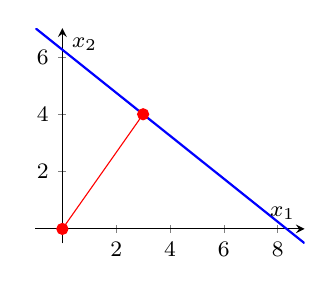
\begin{tikzpicture}
  \begin{axis}[footnotesize,font=\footnotesize
  ,xlabel={$x_1$}, ylabel={$x_2$}
  ,axis lines=middle ,samples=2 ,domain=-1:9]
  \addplot[blue,no marks,thick]{(25-3*x)/4};
  \addplot[red,mark=*] coordinates {(0,0)(3,4)};
  \end{axis}
\end{tikzpicture}
\end{wrapfigure}
\begin{example}[closest point to the origin] 
What is the point on the line \(3x_1+4x_2=25\) that is closest to the origin?
I am sure you could think of several methods, perhaps inspired by the marginal graph, but here use an \svd\ and \cref{thm:smallsoln}.
Confirm the \script[2] computation~\verb|A\b|\index{A\slosh@\texttt{A\slosh}} gives this same closest point, but \script[1] gives a different `answer' (one that is not relevant here).

\begin{solution} 
The point on the line \(3x_1+4x_2=25\) closest to the origin, is the smallest solution of \(3x_1+4x_2=25\)\,.  
Rephrase as the matrix vector system \(A\xv=b\) for matrix \(A=\begin{bmatrix} 3&4 \end{bmatrix}\) and \(b=25\), and apply \cref{pro:gensol}.
\begin{enumerate}
\item Factorize \(A=\usv\) in \script\ via \verb|[U,S,V]=svd([3 4])|\,:
\begin{verbatim}
U =  1
S =
   5   0
V =
   0.6000  -0.8000
   0.8000   0.6000
\end{verbatim}
\item Solve \(Uz=b=25\) which here gives \(z=25\)\,.
\item Solve \(S\yv=z=25\) with general solution here of \(\yv=(5,y_2)\). 
Obtain the smallest solution with free variable \(y_2=0\)\,.
\item Solve \(\tr V\xv=\yv\) by \(\xv=V\yv=V(5,0)=(3,4)\).  
\end{enumerate}
This is the smallest solution and hence the point on the line closest to the origin (as plotted).

Computing \verb|x=A\b|, which here is simply \verb|x=[3 4]\25|, gives answer \(\xv=(3,4)\) in \script[2]; as determined by the \svd, this point is the closest on the line to the origin.
In \script[1] (R2017b), \verb|x=[3 4]\25| gives \(\xv=(0,6.25)\) which the marginal graph shows is a valid solution, but not the \text{smallest solution.}
\end{solution}
\end{example}
\end{reduce}




\begin{activity}
What is the closest point to the origin of the plane \(2x+3y+6z=98\)\,? 
Use the following \svd:
\begin{equation*}
\begin{bmatrix} 2&3&6 \end{bmatrix}
=\begin{bmatrix} 1 \end{bmatrix}
\begin{bmatrix} 7&0&0 \end{bmatrix}
\tr{\begin{bmatrix} \frac27&-\frac37&-\frac67
\\\frac37&\frac67&-\frac27
\\\frac67&-\frac27&\frac37 \end{bmatrix}}.
\end{equation*}
\actposs[4]{\((4,6,12)\)}{\((2,3,6)\)}{\((-3,6,-2)\)}{\((-12,-4,6)\)}
\end{activity}





\begin{table}
\caption{As well as the \script\ commands and operations listed in \cref{tbl:mtlbpre,tbl:mtlbbasics,tbl:mtlbops,tbl:mtlbmops,tbl:mtlbsvd}  we may invoke these functions for drawing images---functions which are otherwise not needed.\index{Matlab@\textsc{Matlab}|textbf}\index{Octave|textbf}} \label{tbl:mtlbimag}
\hrule
\begin{minipage}{\linewidth}
\begin{itemize}

\item \index{reshape()@\texttt{reshape()}}\verb|reshape(A,p,q)| for a \(m\times n\) matrix\slash vector~\(A\), provided \(mn=pq\)\,, generates a \(p\times q\) matrix with \idx{entries} taken column-wise from~\(A\).  
Either \(p\) or~\(q\) can be~\verb|[]| in which case \script\ uses \(p=mn/q\) or \(q=mn/p\) respectively.

\item \index{colormap()@\texttt{colormap()}}\verb|colormap(gray)| \script\ usually draws graphs with colour, but for many images we need greyscale; this command changes the current figure to 64~shades of grey.  

(\verb|colormap(jet)| is the default, \verb|colormap(hot)| is good for both colour and greyscale reproductions, \verb|colormap('list')| lists the available colormaps you can try.)

\item \index{imagesc()@\texttt{imagesc()}}\verb|imagesc(A)| where \(A\)~is a \(m\times n\) matrix of values draws an \(m\times n\) image in the current figure window using the values of~\(A\) (scaled to fit) to determine the colour from the current colormap (e.g., greyscale).

\item \index{log()@\texttt{log()}}\verb|log(x)| where \(x\)~is a  matrix, vector or scalar computes the natural \idx{logarithm} to the base~\(e\) of each element, and returns the result(s) as a correspondingly sized matrix, vector or scalar.

\item \index{exp()@\texttt{exp()}}\verb|exp(x)| where \(x\)~is a  matrix, vector or scalar computes the \idx{exponential} of each element, and returns the result(s) as a correspondingly sized matrix, vector or scalar.%
\footnote{In advanced linear algebra, for application to differential equations and Markov chains, we define the exponential of a matrix, denoted~\(\exp A\) or~\(e^A\).  
This mathematical function is \emph{not} the same as \script's \texttt{exp(A)}, instead one computes \texttt{expm(A)} to get~\(e^A\).}

\end{itemize}
\end{minipage}
\hrule
\end{table}









%\begin{comment}
%Some applications of the smallest solution: perhaps computer tomography as it needs to to the greyest solution to the data.
%Any image??
%\cite{Anton6} [\S11.18] develops computed tomography but only in the over-measured case.
%\end{comment}

\begin{example}[computed tomography] \label{eg:ctscan}
\ 
\begin{quoted}{\idx{Wikipedia}, 2015}
A \index{CT scan}\textsc{ct}-scan, also called  \idx{X-ray}  \idx{computed tomography} (X-ray \textsc{ct}) or computerized axial {tomography} scan (\textsc{cat} scan), makes use of computer-processed combinations of many X-ray images taken from different angles to produce cross-sectional (tomographic) images (virtual 'slices') of specific areas of a scanned object, allowing the user to see inside the object without cutting.
\footnote{\protect\url{https://en.wikipedia.org/wiki/CT\_scan}}
\end{quoted}
Importantly for medical diagnosis and industrial purposes, the computed tomography answer must not have artificial features.
Artificial features must not be generated because of deficiencies in the measurements.
If there is any ambiguity about the answer, then the answer computed should be the `greyest'---the `greyest' corresponds to the mathematical \idx{smallest solution}.

\def\temp#1{\begin{tikzpicture} 
\begin{axis}[small,axis equal image
  ,axis lines=none,ymax=3.8,ymin=-0.5]
  \addplot[] coordinates {(0,0)(3,0)(3,1)(0,1)(0,2)(3,2)(3,3)(0,3)
  (0,0)(1,0)(1,3)(2,3)(2,0)(3,0)(3,3)};
  \node at (axis cs:0.5,0.5) {$r_3$};
  \node at (axis cs:1.5,0.5) {$r_6$};
  \node at (axis cs:2.5,0.5) {$r_9$};
  \node at (axis cs:0.5,1.5) {$r_2$};
  \node at (axis cs:1.5,1.5) {$r_5$};
  \node at (axis cs:2.5,1.5) {$r_8$};
  \node at (axis cs:0.5,2.5) {$r_1$};
  \node at (axis cs:1.5,2.5) {$r_4$};
  \node at (axis cs:2.5,2.5) {$r_7$};
\ifnum#1>0
  \addplot[blue,quiver={u=4,v=0},-stealth] coordinates {(-0.5,0.5)(-0.5,1.5)(-0.5,2.5)};
  \addplot[blue,quiver={u=0,v=4},-stealth] coordinates {(0.5,-0.5)(1.5,-0.5)(2.5,-0.5)};
  \node[right] at (axis cs:0.5,3.5) {$f_1$};
  \node[right] at (axis cs:1.5,3.5) {$f_2$};
  \node[right] at (axis cs:2.5,3.5) {$f_3$};
  \node[above] at (axis cs:3.5,0.5) {$f_6$};
  \node[above] at (axis cs:3.5,1.5) {$f_5$};
  \node[above] at (axis cs:3.5,2.5) {$f_4$};
\fi
\end{axis}
\end{tikzpicture}}
\needlines7
\begin{wrapfigure}[7]r{0pt} \temp0 \end{wrapfigure}
Let's analyse a toy example, as real-life examples have millions of unknowns and equations.%
\footnote{For those interested in reading further, \cite{Kress2015} [\S8] introduces the advanced, highly mathematical, approach to computerized tomography.}
Suppose we divide a cross-section of a body into nine squares (large pixels) in a \(3\times3\) grid.
Inside each square the body's material has some unknown density represented by transmission factors, \hlist r9\ as shown to the right.
The \textsc{ct}-scan\index{CT scan} is to find these transmission factors.
The factor~\(r_j\) is the fraction of the incident \idx{X-ray} that emerges after passing through the \(j\)th~square: typically, smaller~\(r_i\) corresponds to higher density in \text{the body.}

\needlines8
\begin{wrapfigure}[8]r{0pt} \temp1 \end{wrapfigure}
As indicated next to the right, six \idx{X-ray} measurements are made through the body where \hlist f6\ denote the fraction of energy in the measurements relative to the incident power of the X-ray beam.
Thus we need to solve six equations for the nine unknown transmission factors:
\begin{eqnarray*}
&&
r_1r_2r_3=f_1\,,\quad
r_4r_5r_6=f_2\,,\quad
r_7r_8r_9=f_3\,,\quad
\\&&
r_1r_4r_7=f_4\,,\quad
r_2r_5r_8=f_5\,,\quad
r_3r_6r_9=f_6\,.\quad
\end{eqnarray*}
Turn such \idx{nonlinear equation}s into linear equations that we can handle by taking the \idx{logarithm} (to any base, but here say the \idx{natural logarithm} to base~\(e\)) of both sides of all equations
(computers almost always use ``\idx{log}'' to denote the \idx{natural logarithm}, so we do too.  Herein, unsubscripted ``log'' means the same as ``ln''):
\begin{equation*}
r_ir_jr_k=f_l \iff (\ln r_i)+(\ln r_j)+(\ln r_k)=(\ln f_l).
\end{equation*}
That is, letting new unknowns \(x_i=\ln r_i\) and new right-hand sides \(b_i=\ln f_i\)\,, we solve six linear equations for nine unknowns:
\begin{eqnarray*}&&
x_1+x_2+x_3=b_1\,,\quad
x_4+x_5+x_6=b_2\,,\quad
x_7+x_8+x_9=b_3\,,
\\&&
x_1+x_4+x_7=b_4\,,\quad
x_2+x_5+x_8=b_5\,,\quad
x_3+x_6+x_9=b_6\,.
\end{eqnarray*}
This forms the matrix-vector system \(A\xv=\bv\) for \(6\times9\) matrix
\begin{equation*}
A=\begin{bmatrix} 
 1&1&1&0&0&0&0&0&0 \\
 0&0&0&1&1&1&0&0&0 \\
 0&0&0&0&0&0&1&1&1 \\
 1&0&0&1&0&0&1&0&0 \\
 0&1&0&0&1&0&0&1&0 \\
 0&0&1&0&0&1&0&0&1 \end{bmatrix}.
\end{equation*}
For example, let's find an answer for the factors when the measurements give vector \(\sloppy\bv=(-0.91, -1.04, -1.54, -1.52, -1.43, -0.53)\) (all negative as they are the logarithms of fractions~\(f_i\) less than~one)
\setbox\ajrqrbox\hbox{\qrcode{% simple CT scan
A=[1 1 1 0 0 0 0 0 0 
 0 0 0 1 1 1 0 0 0 
 0 0 0 0 0 0 1 1 1
 1 0 0 1 0 0 1 0 0 
 0 1 0 0 1 0 0 1 0 
 0 0 1 0 0 1 0 0 1 ]
b=[-0.91 -1.04 -1.54 -1.52 -1.43 -0.53]'
x=A\slosh b
r=reshape(exp(x),3,3)
colormap(gray),imagesc(r)
}}%
\marginajrbox%
\begin{verbatim}
A=[1 1 1 0 0 0 0 0 0 
 0 0 0 1 1 1 0 0 0 
 0 0 0 0 0 0 1 1 1
 1 0 0 1 0 0 1 0 0 
 0 1 0 0 1 0 0 1 0 
 0 0 1 0 0 1 0 0 1 ]
b=[-0.91 -1.04 -1.54 -1.52 -1.43 -0.53]'
x=A\b
r=reshape(exp(x),3,3)
colormap(gray),imagesc(r)
\end{verbatim}

\index{colormap()@\texttt{colormap()}}%

\def\temp#1#2#3#4#5#6#7#8#9{\begin{tikzpicture}
\begin{axis}[tiny,axis equal image,colormap/blackwhite,axis lines=none]
\addplot[patch,patch type=rectangle
,point meta min={0},point meta max={1}
,table/row sep=\\,patch table with point meta={%
8 9 13 12   #1\\
4 5 9 8     #2\\
0 1 5 4     #3\\
9 10 14 13  #4\\
5 6 10 9    #5\\
1 2 6 5     #6\\
10 11 15 14 #7\\
6 7 11 10   #8\\
2 3 7 6     #9\\
}]
table[row sep=\\] {
x y \\
0 0\\% 0
1 0\\% 1
2 0\\% 2
3 0\\% 3
0 1\\% 4
1 1\\% 5
2 1\\% 6
3 1\\% 7
0 2\\% 8
1 2\\% 9
2 2\\% 10
3 2\\% 11
0 3\\% 12
1 3\\% 13
2 3\\% 14
3 3\\% 15
};
\end{axis}
\end{tikzpicture}}%
\begin{itemize}
\item 
The answer from \script[2] is \twodp
\begin{equation*}
\xv=
(-.42,-.39,-.09,-.47,-.44,-.14,-.63,-.60,-.30).
\end{equation*}
These are logarithms so to get the corresponding physical transmission factors compute the \idx{exponential} of each component, denoted as \(\exp(\xv)\),
\begin{equation*}
\rv=\exp(\xv)=(.66,.68,.91,.63,.65,.87,.53,.55,.74),
\end{equation*}
although it is perhaps more appealing to put these factors into the shape of the \(3\times3\) array of pixels as in (and as illustrated to the right)
\begin{align*}&
\begin{bmatrix} r_1&r_4&r_7\\r_2&r_5&r_8\\r_3&r_6&r_9 \end{bmatrix}
=\begin{bmatrix} 0.66&0.63&0.53
\\0.68&0.65&0.55
\\0.91&0.87&0.74
 \end{bmatrix}.
&&\raisebox{-5ex}{\temp{0.66}{0.68}{0.91}{0.63}{0.65}{0.87}{0.53}{0.55}{0.74}}
\end{align*}
\script[2]'s answer predicts that there is less transmitting, more absorbing, denser, material to the top-right; and more transmitting, less absorbing, less dense, material to the bottom-left.

\item 
However, the answer from \script[1]'s \verb|A\b|\index{A\slosh@\texttt{A\slosh}} is \twodp
\begin{equation*}
\xv=\small(-0.91,0,0,-0.61,-1.43,1.01,0,0,-1.54),
\end{equation*}
as illustrated below in the leftmost picture.  This is quite a different answer!%
\footnote{\script[1] does give a warning in this instance (\index{Rank deficient, \ldots@\texttt{Rank deficient, \ldots}}\texttt{Warning: Rank deficient, \ldots}), but it does not always. 
For example, it does not warn of issues when you ask it to solve \(\frac12(x_1+x_2)=3\) via \texttt{[0.5 0.5]\slosh 3}: it simply computes the `answer' \(\xv=(6,0)\).}
\begin{center}
\temp{0.40}{1.00}{1.00}{0.54}{0.24}{2.74}{1.00}{1.00}{0.21}
\hfil
%\temp{0.22}{1.00}{1.85}{1.00}{0.24}{1.48}{1.00}{1.00}{0.21}
%\hfil
\temp{0.22}{1.85}{1.00}{1.00}{0.35}{1.00}{1.00}{0.37}{0.59}
\hfil
\temp{0.40}{1.00}{1.00}{1.48}{0.24}{1.00}{0.37}{1.00}{0.59}
\hfil
\temp{0.22}{0.67}{2.74}{1.00}{0.35}{1.00}{1.00}{1.00}{0.21}
\end{center}
Furthermore, \script[1] could give other `answers' as illustrated in the other pictures above. 
Reordering the rows in the matrix~\(A\) and right-hand side~\bv\  does not change the system of equations.
But after such reordering the answer from \script[1]'s \verb|x=A\b|\index{A\slosh@\texttt{A\slosh}}  variously predicts each of the above \text{four pictures.}
\end{itemize}


The reason for such multiplicity of mathematically valid answers is that the problem is underdetermined.  
There are nine unknowns but only six equations, so in linear algebra there are typically an infinity of valid answers (as in \cref{thm:feweqns}): just five of these are illustrated above.
\emph{In this application to \textsc{ct}-scans} we add the additional information that we desire the answer that is the `greyest', the most `washed out', the answer with fewest features.
Finding the answer~\xv\ that minimizes~\(|\xv|\) is a reasonable way to quantify this desire.%
\footnote{Another possibility is to increase the number of measurements in order to increase the number of equations to match the number of unknown pixels.
However, measurements are often prohibitively expensive.
Further, increasing the number of measurements tempts us to increase the resolution by having more smaller pixels: in which case we again have to deal with the same issue of more variables than known equations.}

The \svd\ procedure guarantees that we find such a smallest answer.
\cref{pro:appsol} in \script\ gives the following process to satisfy the experimental measurements expressed in \(A\xv=\bv\)\,.
\begin{enumerate}
\item First, find an \svd, \(A=\usv\), via \verb|[U,S,V]=svd(A)| and get \twodp
\setbox\ajrqrbox\hbox{\qrcode{% svd CT scan
[U,S,V]=svd(A)
z=U'*b
y=z(1:5)./diag(S(1:5,1:5))
x=V(:,1:5)*y
}}%
\marginajrbox%
\begin{small}
\begin{verbatim}
U =
 -0.41 -0.00  0.82 -0.00  0.00  0.41
 -0.41 -0.00 -0.41 -0.57 -0.42  0.41
 -0.41 -0.00 -0.41  0.57  0.42  0.41
 -0.41  0.81 -0.00  0.07 -0.09 -0.41
 -0.41 -0.31 -0.00 -0.45  0.61 -0.41
 -0.41 -0.50  0.00  0.38 -0.52 -0.41
S =
  2.45     0     0     0     0     0     0     0     0
     0  1.73     0     0     0     0     0     0     0
     0     0  1.73     0     0     0     0     0     0
     0     0     0  1.73     0     0     0     0     0
     0     0     0     0  1.73     0     0     0     0
     0     0     0     0     0  0.00     0     0     0
V =
 -0.33  0.47  0.47  0.04 -0.05  0.03 -0.58 -0.21 -0.25
 -0.33 -0.18  0.47 -0.26  0.35 -0.36  0.49 -0.27 -0.07
 -0.33 -0.29  0.47  0.22 -0.30  0.33  0.09  0.47  0.33
 -0.33  0.47 -0.24 -0.29 -0.29 -0.48  0.11  0.37  0.26
 -0.33 -0.18 -0.24 -0.59  0.11  0.41 -0.24 -0.27  0.38
 -0.33 -0.29 -0.24 -0.11 -0.54  0.07  0.13 -0.10 -0.64
 -0.33  0.47 -0.24  0.37  0.19  0.45  0.47 -0.16 -0.00
 -0.33 -0.18 -0.24  0.07  0.59 -0.05 -0.25  0.53 -0.31
 -0.33 -0.29 -0.24  0.55 -0.06 -0.40 -0.22 -0.37  0.32
\end{verbatim}
\end{small}


\item Solve \(U\zv=\bv\) by \verb|z=U'*b| to find
\begin{equation*}
\zv=(2.85,-0.52, 0.31, 0.05,-0.67,-0.00).
\end{equation*}

\item Because the sixth \idx{singular value} is zero, ignore the sixth equation: because \(z_6=0.00\) \twodp\ this is only a small inconsistency error.
Now set $y_i=z_i/\sigma_i$ for \(i=1,\ldots,5\) and \emph{for the smallest magnitude answer set the free variables} \(y_6=y_7=y_8=y_9=0\) (\cref{thm:smallsoln}).
Obtain the nonzero values via \verb|y=z(1:5)./diag(S(1:5,1:5))| to find
\begin{equation*}
\yv=(1.16,-0.30, 0.18, 0.03,-0.39,0,0,0,0)
\end{equation*}

\item 
\begin{figbox}{\temp{0.66}{0.68}{0.91}{0.63}{0.65}{0.87}{0.53}{0.55}{0.74}}
Then,  via \verb|x=V(:,1:5)*y|, solve \(\tr V\xv=\yv\) to determine the \idx{smallest solution} is
\(\sloppy\xv= (-0.42,-0.39,-0.09,-0.47,-0.44,-0.14,-0.63,-0.60,-0.30)\).
This is the same answer as computed by \script[2]'s \verb|A\b| to give the pixel image shown that has minimal artifices.
\end{figbox}
\end{enumerate}
In practice, \emph{each} slice of a real \textsc{ct}-scan\index{CT scan} would involve finding the absorption of tens of millions of pixels.
That is, a \textsc{ct}-scan needs to best solve many systems of tens of millions of equations in tens of millions of unknowns!
\end{example}



%\begin{example}[one layer neural network] 
%Not appropriate here.
%
%Artificial \idx{neural network}s are often invoked in machine learning, artificial intelligence, knowledge discovery, and data mining.
%In essence, neural networks attempt to fit data (knowledge) by a computational procedure---one that can be understood mathematically.
%A common computational model of a neuron is that of the \idx{sigmoidal function} \(g(x)=1/(1+e^{-x})\) as plotted to the right.
%\marginpar{%
%\begin{tikzpicture}[baseline]
%  \begin{axis}[footnotesize,font=\footnotesize
%  ,xlabel={$x$}, ylabel={$1/(1+e^{-x})$}
%  ,axis x line=middle , axis y line=middle
%  ,thick,samples=21
%  ,domain=-6:6,ymin=0,ymax=1.3
%  ]
%  \addplot[blue,no marks]{1/(1+exp(-x))};
%  \end{axis}
%\end{tikzpicture}
%}%
%Perhaps the simplest nontrivial neural network is a single layer network with a single input: mathematically we put \(n\)~neurons in a single layer with combined output by seeking a function of the form
%\begin{equation*}
%y=c_1g(a_1x-b_1)+c_2g(a_2x-b_2)+\cdots+c_ng(a_nx-b_n).
%\end{equation*}
%??
%\end{example}





\needspace{9\baselineskip}
\subsection{Orthogonal projection resolves vector components}
\label{sec:proj}
\index{orthogonal projection|(}


\begin{comment}
\cite[p.738]{HughesHallett2013} \pooliv{p.27--8}
onto a vector, parallel and perpendicular components, work done
\pooliv{p.382}
orthogonal projections onto subspace, orthogonal decomposition thm,
\end{comment}

Reconsider the task of making a minimal change to the right-hand side of a \idx{system} of \idx{linear equation}s, and let's connect it to the so-called orthogonal projection.
This important connection occurs because of the geometry that the closest point on a line or plane to another given point is the one which forms a right-angle; that is, it forms an \text{orthogonal vector.}

This optional section does usefully support least square approximation, and provides examples of transformations for the next \cref{sec:ilt}.
Such orthogonal projections are extensively used in applications.


\needlines6
\subsubsection{Project onto a direction}
%\label{sec:poad}

\begingroup% delimits definition of \temp
\newcommand{\temp}[1]{\begin{tikzpicture}
  \begin{axis}[footnotesize,font=\footnotesize
  ,axis equal image,axis lines=middle
  ,samples=2 ,domain=-1:9]
  \addplot[blue,no marks]{x/2};
  \addplot[blue,very thick,quiver={u=2,v=1},-stealth]coordinates {(0,0)};
  \node[below] at (axis cs:2,1) {$\av$};
  \addplot[red,quiver={u=3,v=4},-stealth]coordinates {(0,0)};
  \node[right] at (axis cs:3,4) {$\bv$};
  \ifnum#1>0
  \addplot[red,mark=*] coordinates {(3,4)(4,2)};
  \node[below] at (axis cs:4,2) {$\bv'$};
  \fi
  \ifnum#1>1
  \node[left] at (axis cs:2,3) {$|\bv|$};
  \node[above] at (axis cs:1.5,0.75) {$\theta$};  
  \fi
  \ifnum#1>2
  \addplot+[yellow!95!black,mark=*,mark size=6] coordinates {(1,8)};
  \fi
  \end{axis}
\end{tikzpicture}}
\begin{wrapfigure}r{0pt} \temp0 \end{wrapfigure}
\begin{example} \label{eg:incon1}
Consider `solving' the \idx{inconsistent system} \(\av x=\bv\) where \(\av=(2,1)\) and \(\bv=(3,4)\); that is, solve
\begin{equation*}
\begin{bmatrix} 2\\1 \end{bmatrix}x=\begin{bmatrix} 3\\4 \end{bmatrix}.
\end{equation*}
As illustrated to the right, the impossible task is to find some multiple of the vector \(\av=(2,1)\) (all multiples plotted) that equals \(\bv=(3,4)\).
It cannot be done.
Question: how may we change the right-hand side vector~\bv\ so that the task is possible?  
A partial answer is to replace~\bv\ by some vector~\(\bv'\) which is in the \idx{column space} of matrix \(A=\begin{bmatrix} \av \end{bmatrix}\).
But we could choose any~\(\bv'\) in the column space, so any answer for the multiple~\(x\) would be possible! Surely any answer is not acceptable.

\begin{wrapfigure}r{0pt} \temp1 \end{wrapfigure}
Instead, often the preferred answer is, out of all vectors in the column space of matrix \(A=\begin{bmatrix} \av \end{bmatrix}\),  find the vector~\(\bv'\) in the column space \emph{which is closest to}~\bv---as illustrated to the right here where it looks like \(\bv'=(4,2)\).

The \svd\ approach of \cref{pro:appsol} to find~\(\bv'\) and~\(x\) is the following.
\begin{enumerate}
\item Use \verb|[U,S,V]=svd([2;1])| to find here the \svd\ factorization \begin{equation*}
A=\usv=\begin{bmatrix} 0.89&-0.45\\0.45&0.89 \end{bmatrix} \begin{bmatrix} 2.24\\0 \end{bmatrix}\tr{\begin{bmatrix} 1 \end{bmatrix}}\quad \twodp.
\end{equation*}
\item Then \(\zv=\tr U\bv=(4.47,2.24)\).
\item Treat the second component of \(Sy=\zv\) as an error---it is the magnitude \(|\bv-\bv'|\)---to deduce \(y=4.47/2.24=2.00\) \twodp\ from the first component.
\item Then  \(x=Vy=1y=2\) solves the changed problem.
\end{enumerate}
From this solution, the vector \(\bv'=\av x=(2,1)2=(4,2)\), as is recognizable in the graphs.
\end{example}

\begin{wrapfigure}r{0pt} \temp2 \end{wrapfigure}
Now let's derive the same result but with two differences:
firstly, use more elementary arguments, not the \svd; 
and secondly, derive the result for general vectors~\av\ and~\bv\ (although continuing to use the same illustration).
Start with the crucial observation that the closest point\slash vector~\(\bv'\) in the \idx{column space} of \(A=\begin{bmatrix} \av \end{bmatrix}\) is such that \(\bv-\bv'\) is at \idx{right-angles}, orthogonal, to~\av.
(If \(\bv-\bv'\) were not orthogonal, then we would be able to slide~\(\bv'\) along the line \(\Span\{\av\}\) to reduce the \idx{length} of \(\bv-\bv'\).)
Thus we form a right-angle triangle with hypotenuse of length~\(|\bv|\) and angle~\(\theta\) as shown to the right.
Trigonometry then gives the adjacent length \(|\bv'|=|\bv|\cos\theta\)\,.
But the angle~\(\theta\) is that between the given vectors~\av\ and~\bv, so the dot product gives the \idx{cosine} as \(\cos\theta={\av\cdot\bv}/({|\av||\bv|})\)  (\cref{thm:anglev}).
Hence the adjacent length \begin{equation*}
|\bv'|=|\bv|\cos\theta
=|\bv|\frac{\av\cdot\bv}{|\av||\bv|}=\frac{\av\cdot\bv}{|\av|}\,.
\end{equation*}
To approximately solve \(\av x=\bv\)\,, replace the inconsistent \(\av x=\bv\) by the \idx{consistent} \(\av x=\bv'\)\,.
Then as \(x\) is a scalar we solve this consistent equation via the ratio of lengths,  \(x=|\bv'|/|\av|={\av\cdot\bv}/|\av|^2\).
For \cref{eg:incon1}, this gives `solution' \(x=(2,1)\cdot(3,4)/(2^2+1^2)=10/5=2\) \text{as before.}

\needlines8
\begin{wrapfigure}[7]r{0pt} \temp3 \end{wrapfigure}
A crucial part of such solutions is the general formula for \(\bv'=\av x=\av(\av\cdot\bv)/|\av|^2\).
Geometrically the formula gives the `shadow'~\(\bv'\) of vector~\bv\ when projected by a `sun' high above the line of the vector~\av, as illustrated schematically to the right.
As such, the formula is called an \text{orthogonal projection.}
\vspace{1\baselineskip}

\endgroup% delimits definition of \temp



\begin{definition}[orthogonal projection onto 1D] \label{def:orthproj1}
Let \(\uv,\vv\in\RR^n\) and vector \(\uv\neq\ov\)\,, then the \bfidx{orthogonal projection} of~\vv\ onto~\uv\ is
\begin{subequations}\label{eqs:}%
\begin{equation}
\proj_\uv(\vv):=\uv\frac{\uv\cdot\vv}{|\uv|^2}\,.
\label{eq:orthproj1a}
\end{equation}
In the special but common case when~\uv\ is a \idx{unit vector},
\begin{equation}
\proj_\uv(\vv):=\uv(\uv\cdot\vv).
\label{eq:orthproj1b}
\end{equation}
\end{subequations}
\end{definition}


\newcommand{\projuv}[9]{\begin{tikzpicture}
  \begin{axis}[footnotesize%,font=\footnotesize
  ,axis equal ,axis x line=none , axis y line=none
  ,samples=2 ]
  \addplot[black,mark=*]coordinates {(0,0)};
  \addplot[red,quiver={u=#1,v=#2},-stealth]coordinates {(0,0)};
  \node[right] at (axis cs:#1,#2) {$\vec #9$};
  \addplot[blue,quiver={u=#3,v=#4},-stealth]coordinates {(0,0)};
  \node[right] at (axis cs:#3,#4) {$\vec #8$};
  \ifnum#7>0
  \addplot[red,mark=*] coordinates {(#1,#2)(#5,#6)};
  \node[right] at (axis cs:#5,#6) {$\proj_{\vec #8}(\vec #9)$};
  \addplot[brown,thick,quiver={u=#5,v=#6},-stealth]coordinates {(0,0)};
  \fi
  \end{axis}
\end{tikzpicture}}
\begin{example} 
For the following pairs of vectors: draw the named orthogonal projection; and for the given \idx{inconsistent system}, determine whether the `best' \idx{approximate solution} is in the range \(x<-1\)\,, \(-1<x<0\)\,, \(0<x<1\)\,, or \(1<x\)\,.
\begin{Parts}
\item \(\proj_\uv(\vv)\) and \(\uv x=\vv\)\\
\projuv4134{1.92}{2.56}0uv
\item \(\proj_\qv(\pv)\) and \(\qv x=\pv\)\\
\projuv132{-2}{-1}{1}0qp
\end{Parts}
\begin{solution} \ \\
\begin{Parts}
\item \projuv4134{1.92}{2.56}1uv\\
Draw a line perpendicular to~\uv\ that passes through the tip of~\vv.
Then \(\proj_\uv(\vv)\) is the shown brown vector.
To `best solve' \(\uv x=\vv\)\,, approximate the equation \(\uv x=\vv\) by \(\uv x=\proj_\uv(\vv)\).
Since \(\proj_\uv(\vv)\) is smaller than~\uv\ and the same direction, \(0<x<1\)\,.
\aqed

\item \projuv132{-2}{-1}{1}1qp\\
Vector~\qv\ in \(\proj_\qv(\pv)\) gives the direction of a line, so we can and do project onto the negative direction of~\qv.
To `best solve' \(\qv x=\pv\)\,, approximate the equation \(\qv x=\pv\) by \(\qv x=\proj_\qv(\pv)\).
Since the brown vector \(\proj_\qv(\pv)\) is smaller than~\qv\ and in the opposite direction, \(-1<x<0\)\,.
\aqed

\end{Parts} 
\end{solution}
\end{example}




\begin{example} \label{eg:projline}
For the following pairs of vectors: 
compute the given orthogonal projection; 
and hence find the `best' \idx{approximate solution} to the given \idx{inconsistent system}.
\begin{enumerate}
\item Find \(\proj_\uv(\vv)\) for vectors \(\uv=(3,4)\) and \(\vv=(4,1)\), and hence best solve \(\uv x=\vv\)\,.
\begin{solution} 
\begin{equation*}
\proj_\uv(\vv)=(3,4)\frac{(3,4)\cdot(4,1)}{|(3,4)|^2}
=(3,4)\frac{16}{25}
=(\tfrac{48}{25},\tfrac{64}{25}).
\end{equation*}
Approximate equation \(\uv x=\vv\) by \(\uv x=\proj_\uv(\vv)\), that is, \((3,4)x=(\tfrac{48}{25},\tfrac{64}{25})\) with solution \(x=\tfrac{16}{25}\) (from either component, or the ratio of lengths).
\end{solution}

\begin{reduce}
\item Find \(\proj_\sv(\rv)\) for vectors \(\rv=(1,3)\) and \(\sv=(2,-2)\), and hence best solve \(\sv x=\rv\)\,.
\begin{solution} 
\begin{equation*}
\proj_\sv(\rv)=(2,-2)\frac{(2,-2)\cdot(1,3)}{|(2,-2)|^2}
=(2,-2)\frac{-4}{8}
=(-1,1).
\end{equation*}
Approximate equation \(\sv x=\rv\) by \(\sv x=\proj_\sv(\rv)\), that is, \((2,-2)x=(-1,1)\) with solution \(x=-1/2\)  (from either component, or the ratio of lengths).
\end{solution}
\end{reduce}

\item Find \(\proj_\pv(\qv)\) for vectors \(\pv=(\tfrac13,\tfrac23,\tfrac23)\) and \(\qv=(3,2,1)\), and best solve \(\pv x=\qv\)\,.
\begin{solution} 
Vector~\pv\ is a unit vector, so we use the simpler formula that
\begin{eqnarray*}
\proj_\pv(\qv)&=& (\tfrac13,\tfrac23,\tfrac23)\big[(\tfrac13,\tfrac23,\tfrac23)\cdot(3,2,1)\big]
\\&=&(\tfrac13,\tfrac23,\tfrac23)\big[1+\tfrac43+\tfrac23\big] 
\\&=&(\tfrac13,\tfrac23,\tfrac23)3
=(1,2,2).
\end{eqnarray*}
Then `best solve' equation \(\pv x=\qv\) by the approximation \(\pv x=\proj_\pv(\qv)\), that is, \((\tfrac13,\tfrac23,\tfrac23)x=(1,2,2)\) with solution \(x=3\) (from any component, or the ratio of lengths).
\end{solution}
\end{enumerate}
\end{example}




\begin{activity}
Use projection to best solve the inconsistent equation \((1,4,8)x=(4,4,2)\). 
The best answer is which of the following?
\actposs[4]{\(x=4/9\)}{\(x=10/13\)}{\(x=4\)}{\(x=21/4\)}
\end{activity}











\subsubsection{Project onto a subspace}
\index{subspace|(}

The previous subsection develops a geometric view of the `best' solution to the \idx{inconsistent system} \(\av x=\bv\)\,.
The discussion introduced that the conventional `best' solution---that determined by \cref{pro:appsol}---is to replace~\bv\ by its projection~\(\proj_{\av}(\bv)\), namely to solve \(\av x=\proj_{\av}(\bv)\).
The rationale is that this is the \emph{smallest} change to the right-hand side~\bv\ that enables the equation to be solved.  
This subsection introduces that solving inconsistent equations in more variables may be viewed as an analogous projection onto \text{a subspace.}



\begin{definition}[project onto a subspace] \label{def:orthproj}
Let \WW\ be a \(k\)-\idx{dimension}al \idx{subspace} of~\(\RR^n\) with an \idx{orthonormal basis} \(\{\hlist\wv k\}\).
For every vector \(\vv\in\RR^n\), the \bfidx{orthogonal projection} of vector~\vv\ onto subspace~\WW\ is
\begin{equation*}
\proj_\WW(\vv)=\wv_1(\wv_1\cdot\vv)+\wv_2(\wv_2\cdot\vv)+\cdots+\wv_k(\wv_k\cdot\vv).
%\label{eq:orthproj}
\end{equation*}
\end{definition}

\begin{example} \label{eg:orthproj}
\begin{enumerate}[ref=\ref{eg:orthproj}(\alph*)]
\item 
Let \XX\ be the \(xy\)-plane in \(xyz\)-space, find \(\proj_\XX(3,-4,2)\).

\begin{figbox}{\qview{58}{62}{\begin{tikzpicture} 
\begin{axis}[footnotesize,axis equal image
,font=\footnotesize,view={\q}{20}
,xlabel={$x$},ylabel={$y$},zlabel={$z$},label shift={-2ex}
,domain=0:5,y domain=-5:0]
    \addplot3[surf,blue,opacity=0.3,samples=2] {0};
    \addplot3[quiver={u=3,v=-4,w=2},red,-stealth,thick] 
    coordinates {(0,0,0)};
    \node[right,red] at (axis cs:3,-4,2) {$(3,-4,2)$};
    \addplot3[red,dotted] coordinates {(3,-4,2)(3,-4,0)};
    \addplot3[quiver={u=3,v=-4,w=0},brown,-stealth,thick] 
    coordinates {(0,0,0)};
    \node[right,brown] at (axis cs:3,-4,0) {$(3,-4,0)$};
\end{axis}
\end{tikzpicture}}}
\begin{solution} 
An orthonormal basis for the \(xy\)-plane (blue plane in the stereo picture to the right) are the two unit vectors \(\iv=(1,0,0)\) and \(\jv=(0,1,0)\). 
Hence
\begin{align*}
\proj_\WW(3,-4,2)
&=\iv(\iv\cdot(3,-4,2))+\jv(\jv\cdot(3,-4,2))
\\&=\iv (3+0+0)+\jv (0-4+0) 
\\&=(3,-4,0)
\qquad(\text{shown in brown}).
\end{align*}
That is, just set the third component of~\((3,-4,2)\) to zero.
\end{solution}
\end{figbox}


%\item Set subspace \(\WW=\Span\{(1,2,2)\clb (2,1,-2)\}\) and determine \(\proj_\WW(3,-4,2)\).
%\begin{solution} 
%Although the two vectors in the span are orthogonal (blue to the rightal picture), they are not unit vectors.  
%Normalize the vectors by dividing by their length \(\sqrt{1^2+2^2+2^2}=\sqrt{2^2+1^2+(-2)^2}=3\) to find the vectors \(\wv_1=(\frac13,\frac23,\frac23)\) and  \(\wv_2=(\frac23,\frac13,-\frac23)\) are an orthonormal basis for~\WW\ (blue plane).
%\marginpar{\begin{tikzpicture} 
%\begin{axis}[footnotesize,axis equal image,font=\tiny,view={65}{30}
%,domain=-1:3,y domain=-4:2,zmax=2,zmin=-2]
%    \addplot3[quiver={u=1,v=2,w=2},blue,-stealth,thick] 
%    coordinates {(0,0,0)};
%    \addplot3[quiver={u=2,v=1,w=-2},blue,-stealth,thick] 
%    coordinates {(0,0,0)};
%    \addplot3[surf,blue,opacity=0.3,samples=2] {-2*x+2*y};
%    \addplot3[quiver={u=3,v=-4,w=2},red,-stealth,thick] 
%    coordinates {(0,0,0)};
%    \node[below,red,font=\tiny] at (axis cs:3,-4,2) {$\quad(3,-4,2)$};
%    \addplot3[red,dotted] coordinates {(3,-4,2)(-5/9,-4/9,2/9)};
%    \addplot3[quiver={u=-5/9,v=-4/9,w=2/9},brown,-stealth,thick] 
%    coordinates {(0,0,0)};
%\end{axis}
%\end{tikzpicture}}
%Hence 
%\begin{eqnarray*}
%&&\proj_\WW(3,-4,2)
%\\&=&\wv_1(\wv_1\cdot(3,-4,2))+\wv_2(\wv_2\cdot(3,-4,2))
%\\&=&\wv_1(1-\tfrac83+\tfrac43)+\wv_2(2-\tfrac43-\tfrac43)
%\\&=&-\tfrac13\wv_1-\tfrac23\wv_2
%\\&=&-\tfrac13(\tfrac13,\tfrac23,\tfrac23)-\tfrac23(\tfrac23,\tfrac13,-\tfrac23)
%\\&=&\tfrac19(-5,-4,2).
%\end{eqnarray*}
%\end{solution}
%
\item 
\def\temp#1{\qview{73}{77}{\begin{tikzpicture} 
\begin{axis}[small,axis equal image
,font=\footnotesize,view={\q}{30}
,domain=0:3,y domain=-2:2,zmax=1,zmin=-2]
    \addplot3[quiver={u=2,v=-2,w=1},blue,-stealth,thick] 
    coordinates {(0,0,0)};
    \addplot3[quiver={u=2,v=1,w=-2},blue,-stealth,thick] 
    coordinates {(0,0,0)};
    \addplot3[surf,opacity=0.3,samples=9] {-x/2-y};
    \addplot3[quiver={u=3,v=2,w=1},red,-stealth,thick] 
    coordinates {(0,0,0)};
    \node[above,red] at (axis cs:3,1,1) {$(3,2,1)\ $};
\ifnum#1=2
    \addplot3[red,dotted] coordinates {(3,2,1)(2,0,-1)};
    \addplot3[quiver={u=2,v=0,w=-1},brown,-stealth,thick] 
    coordinates {(0,0,0)};
\fi
\end{axis}
\end{tikzpicture}}}%

\begin{figbox}{\temp1}
For the subspace \(\WW=\Span\{(2,-2,1)\clb (2,1,-2)\}\), determine the \(\proj_\WW(3,2,1)\) (illustrated to the right).
\end{figbox}

\begin{figbox}{\temp2}
\begin{solution} 
Although the two vectors in the span are orthogonal (blue in the stereo picture above), they are not unit vectors.  
Normalize the vectors by dividing by their length \(\sqrt{2^2+(-2)^2+1^2}=\sqrt{2^2+1^2+(-2)^2}=3\) to find the vectors \(\wv_1=(\frac23,-\frac23,\frac13)\) and  \(\wv_2=(\frac23,\frac13,-\frac23)\) are an orthonormal basis for~\WW\ (a plane).
Hence 
\begin{align*}
\proj_\WW(3,2,1)
&=\wv_1(\wv_1\cdot(3,2,1))+\wv_2(\wv_2\cdot(3,2,1))
\\&=\wv_1(2-\tfrac43+\tfrac13)
+\wv_2(2+\tfrac23-\tfrac23)
\\&=\wv_1+2\wv_2
\\&=(\tfrac23,-\tfrac23,\tfrac13)+2(\tfrac23,\tfrac13,-\tfrac23)
\\&=(2,0,-1) 
\qquad(\text{shown in brown}).
\end{align*}%
\end{solution}
\end{figbox}

\item\label[example]{eg:orthproj:iii} Recall the \idx{table tennis} ranking \cref{eg:rstp2,eg:rstp3}.
To rank the players we seek to solve the matrix-vector system, $A\xv=\bv$\,,
    \begin{displaymath}
        \begin{bmatrix}
            1&-1&0\\ 1&0&-1\\ 0&1&-1
        \end{bmatrix}\xv=
        \begin{bmatrix}
            1\\ 2\\ 2
        \end{bmatrix}.
    \end{displaymath}
Letting \AA~denote the \idx{column space} of matrix~\(A\), determine \(\proj_\AA(\bv)\).
\begin{solution} \
\def\temp#1{\qview{18}{22}{\begin{tikzpicture} 
\begin{axis}[axis equal image,view={\q}{30}
,small,font=\footnotesize,zmin=-2,zmax=2]
    \addplot3[surf,domain=-1:2,y domain=-1:3,opacity=0.3,samples=9] {y-x};
\def\threevcol{red}
\threev[right]121{\bv}
\ifnum#1=1
    \addplot3[quiver={u=1,v=1,w=0},blue,-stealth,thick] 
    coordinates {(0,0,0)};
    \addplot3[quiver={u=-1,v=0,w=1},blue,-stealth,thick] 
    coordinates {(0,0,0)};
    \addplot3[quiver={u=0,v=-1,w=-1},blue,-stealth,thick] 
    coordinates {(0,0,0)};
\else
    \addplot3[quiver={u=0.408,v=-0.408,w=-0.816},blue,-stealth,thick] 
    coordinates {(0,0,0)};
    \node[below,blue] at (axis cs:0.408,-0.408,-0.816) {$\uv_1$};
    \addplot3[quiver={u=-0.707,v=-0.707,w=0},blue,-stealth,thick] 
    coordinates {(0,0,0)};
    \node[below,blue] at (axis cs:-0.707,-0.707,0) {$\uv_2$};
\fi
\ifnum#1=3
    \addplot3[red,dotted] coordinates {(1,2,1)(2/3,7/3,5/3)};
    \addplot3[quiver={u=2/3,v=7/3,w=5/3},brown,-stealth,thick] 
    coordinates {(0,0,0)};
\fi
\end{axis}
\end{tikzpicture}}}%

\begin{figbox}{\temp1}
We need to find an orthonormal basis for the column space (the illustrated plane spanned by the three shown column vectors)---an \svd\ gives it to us.
\cref{eg:rstp} found an \svd\  \(A=\usv\), in \script\ via  \verb|[U,S,V]=svd(A)|, to be
\end{figbox}
\begin{verbatim}
U =
    0.4082   -0.7071    0.5774
   -0.4082   -0.7071   -0.5774
   -0.8165   -0.0000    0.5774
S =
    1.7321         0         0
         0    1.7321         0
         0         0    0.0000
V =
    0.0000   -0.8165    0.5774
   -0.7071    0.4082    0.5774
    0.7071    0.4082    0.5774
\end{verbatim}
\begin{figbox}{\temp2}
Since there are only two nonzero singular values, the column space~\AA\ is 2D and spanned by the first two orthonormal columns of matrix~\(U\):
that is, an orthonormal basis for~\AA\ is the two vectors (as illustrated)
\begin{eqnarray*}
&&\uv_1=\begin{bmatrix} 0.4082\\-0.4082\\-0.8165 \end{bmatrix}
=\frac1{\sqrt6}\begin{bmatrix} 1\\-1\\-2 \end{bmatrix},
\\&&\uv_2=\begin{bmatrix} -0.7071\\-0.7071\\-0.0000 \end{bmatrix}
=\frac1{\sqrt2}\begin{bmatrix} -1\\-1\\0 \end{bmatrix}.
\end{eqnarray*}
\end{figbox}

\begin{figbox}{\temp3}
Hence the projection of the right-hand side~\bv\ onto the column space~\AA\ is
\begin{align*}
&\proj_\AA(1,2,2)
\\&=\uv_1(\uv_1\cdot(1,2,2))+\uv_2(\uv_2\cdot(1,2,2))
\\&=\uv_1(1-2-4)/\sqrt6
+\uv_2(-1-2+0)/\sqrt2
\\&=-\tfrac5{\sqrt6}\uv_1-\tfrac3{\sqrt2}\uv_2
\\&=\tfrac16(-5,5,10)+\tfrac12(3,3,0)
\\&=\tfrac13(2,7,5) 
\qquad(\text{shown in brown}).
\end{align*}%
\end{figbox}

\end{solution}


\item Find the projection of the vector \((1,2,2)\) onto the plane \(2x-\frac12y+4z=6\)\,.
\begin{solution} 
This plane is not a subspace as it does not pass through the origin.
\cref{def:orthproj} only defines projection onto a subspace so we cannot answer this problem (as yet). 
\end{solution}


\item\label[example]{eg:orthogproj:v} 
\def\temp#1{\qview{63}{67}{\begin{tikzpicture} 
\begin{axis}[small,axis equal image,font=\footnotesize,view={\q}{30}
,xlabel={$x$},ylabel={$y$},zlabel={$z$},label shift={-1.5ex}
,domain=-1.4:1.4,y domain=-0.4:2.4]
    \addplot3[surf,opacity=0.3,samples=9] {-1/2*x+y/8};
\def\threevcol{red}\threevec[left]122
\ifnum#1>1
    \addplot3[quiver={u=0.111,v=0.991,w=0.068},blue,-stealth,thick] 
    coordinates {(0,0,0)};
    \node[below,blue] at (axis cs:0.111,0.991,0.068) {$\uv_2$};
    \addplot3[quiver={u=-0.889,v=0.068,w=0.453},blue,-stealth,thick] 
    coordinates {(0,0,0)};
    \node[right,blue] at (axis cs:-0.889,0.068,0.453) {$\uv_3$};
\fi
\ifnum#1=3
    \addplot3[red,dotted] coordinates {(1,2,2)(1/9,10/9,2/9)};
    \addplot3[quiver={u=1/9,v=10/9,w=2/9},brown,-stealth,thick] 
    coordinates {(0,0,0)};
\fi
\end{axis}
\end{tikzpicture}}}%
\begin{figbox}{\temp1}
Use an \svd\ to find the projection of the vector \((1,2,2)\) onto the plane \(2x-\frac12y+4z=0\) (illustrated to the right).
\vspace{3\baselineskip}
\end{figbox}

\begin{solution} 
This plane does pass through the origin so it forms a subspace, call it~\PP\ (illustrated above).
To project we need two orthonormal basis vectors.
Recall that a normal to the plane is its vectors of coefficients, here~\((2,-\tfrac12,4)\), so we need to find two orthonormal vectors which are orthogonal to~\((2,-\tfrac12,4)\).
Further, recall that the columns of an orthogonal matrix are orthonormal (\cref{thm:orthog:ii}), so use an \svd\ to find orthonormal vectors to~\((2,-\tfrac12,4)\).
In \script,  compute an \svd\ with \verb|[U,S,V]=svd([2;-1/2;4])| to find
\setbox\ajrqrbox\hbox{\qrcode{% project onto plane
[U,S,V]=svd([2;-1/2;4])
cs=U(:,2:3)'*[1;2;2]
proj=U(:,2:3)*cs
}}%
\marginajrbox%
\begin{verbatim}
U =
  -0.4444   0.1111  -0.8889
   0.1111   0.9914   0.0684
  -0.8889   0.0684   0.4530
S =
   4.5000
        0
        0
V = -1
\end{verbatim}

\begin{figbox}{\temp2}
The first column~\(\uv_1=(-4,1,-8)/9\) of orthogonal matrix~\(U\) is in the direction of a normal to the plane as it must since it must be in the span of~\((2,-\tfrac12,4)\).
Since matrix~\(U\) is orthogonal, the last two columns (say \(\uv_2\) and~\(\uv_3\), drawn in blue below) are not only orthonormal, but also orthogonal to~\(\uv_1\) and hence an orthonormal basis for the plane~\PP.
\end{figbox}

Hence the projection of the given vector onto the plane is
\begin{align*}
\proj_\PP(1,2,2)
&=\uv_2(\uv_2\cdot(1,2,2))+\uv_3(\uv_3\cdot(1,2,2))
\\&=2.2308\,\uv_2+0.1539\,\uv_3
\\&=2.2308(0.1111,0.9914,0.0684)
\\&{}+0.1539(-0.8889,0.0684,0.4530)
\\&=(0.1111,2.2222,0.2222)
\\&=\tfrac19(1,10,2)
\qquad(\text{shown in brown}).
\end{align*}
\begin{figbox}{\temp3}
This answer may be computed in \script\ via the two dot products \verb|cs=U(:,2:3)'*[1;2;2]|, giving the two coefficients \(2.2308\) and~\(0.1539\), and then the linear combination \verb|proj=U(:,2:3)*cs|\,.
\vspace{1\baselineskip}
\end{figbox}

\end{solution}
\end{enumerate}
\end{example}



\begin{activity}
Determine which of the following is \(\proj_\WW(1,1,-2)\) for the subspace \(\WW=\Span\{(2,3,6), (-3,6,-2)\}\).
\actposs[4]{\((-\frac57,\frac37,-\frac87)\)}
{\((-\frac17,\frac97,\frac47)\)}
{\((\frac17,-\frac97,-\frac47)\)}
{\((\frac57,-\frac37,\frac87)\)}
\end{activity}




\cref{eg:orthproj:iii} determines the orthogonal projection of the given \idx{table tennis} results \(\bv=(1,2,2)\) onto the \idx{column space} of matrix~\(A\) is the vector \(\bv'=\tfrac13(2,7,5)\).
Recall that \cref{eg:rstp3} invokes \cref{pro:appsol} to find the `approximate' solution of the impossible \(A\xv=\bv\) to be \(\xv=(1,\frac13,-\frac43)\).
Now see that \(A\xv
=\big(1-\frac13,1-(-\frac43),\frac13-(-\frac43)\big)
=(\frac23,\frac73,\frac53)
=\bv'\).
That is, the \idx{approximate solution} method of \cref{pro:appsol} solved the problem \(A\xv=\proj_\AA(\bv)\).
The following \cref{thm:lsqproj} confirms that this is no accident: orthogonally projecting the right-hand side onto the column space of the matrix in a system of linear equations is equivalent to solving the system with the \idx{smallest change} to the right-hand side that makes \text{it \idx{consistent}.}


\begin{theorem}[] \label{thm:lsqproj}
The `\idx{least square}' solution/s of the \idx{system} \(A\xv=\bv\) determined by \cref{pro:appsol} is/are the solution/s of \(A\xv=\proj_{\AA}(\bv)\) where \AA~denotes the \idx{column space} of~\(A\).
\end{theorem}

\begin{proof} 
For any \(m\times n\) matrix~\(A\), \cref{pro:appsol} first finds an \svd\ \(A=\usv\) and sets \(r=\rank A\)\,.
Second, it computes \(\zv=\tr U\bv\) but disregards~\(z_i\) for \(i=r+1,\ldots,m\) as errors.
%Such disregard is equivalent to setting \(z_i=0\) for \(i=r+1,\ldots,m\) instead of using the \(z_i\)~determined from~\bv.
That is, instead of using \(\zv=\tr U\bv\), \cref{pro:appsol} solves the equations with \(\zv'=(\hlist zr,0,\ldots,0)\). 
%Let \(m\times r\)~matrix \(W=\begin{bmatrix} \uv_1&\uv_2&\cdots&\uv_r \end{bmatrix}\) be the first \(r\)~columns of~\(U\).
This vector~\(\zv'\) corresponds to a modified right-hand side~\(\bv'\) satisfying \(\zv'=\tr U\bv'\); that is, \(\bv'=U\zv'\) as matrix~\(U\) is orthogonal.
Recalling \(\uv_i\)~denotes the \(i\)th~column of~\(U\) and that components \(z_i=\uv_i\cdot\bv\) from  \(\zv=\tr U\bv\),
the matrix-vector product \(\bv'=U\zv'\) is the linear combination (\cref{eg:lcmatvec})
\begin{eqnarray*}
\bv'&=&\uv_1z'_1+\uv_2z'_2+\cdots+\uv_rz'_r+\uv_{r+1}0+\cdots+\uv_m0
\\&=&\uv_1(\uv_1\cdot\bv)+\uv_2(\uv_2\cdot\bv)+\cdots+\uv_r(\uv_r\cdot\bv)
\\&=&\proj_{\Span\{\hlist\uv r\}}(\bv),
\end{eqnarray*}
by \cref{def:orthproj} since the columns~\(\uv_i\) of~\(U\) are orthonormal (\cref{thm:orthog}).
\cref{thm:rowcolD} establishes that this span is the column space~\AA\ of matrix~\(A\).
Hence, \(\bv'=\proj_\AA(\bv)\) and so \cref{pro:appsol} solves the system \(A\xv=\proj_\AA(\bv)\).
\end{proof}


\begin{example} \label{eg:fourwts2}
Recall \cref{eg:fourwts} rationalizes four apparently contradictory weighings: in~kg the weighings are~\(84.8\), \(84.1\), \(84.7\) and~\(84.4\)\,.
Denoting the `uncertain' weight by~\(x\),  we write these weighings as the inconsistent matrix-vector system
\begin{equation*}
Ax=\bv\,,\quad\text{namely }
\begin{bmatrix} 1\\1\\1\\1 \end{bmatrix}x
=\begin{bmatrix} 84.8\\84.1\\84.7\\84.4 \end{bmatrix}.
\end{equation*}
Let's see that the orthogonal projection of the right-hand side onto the \idx{column space} of~\(A\) is the same as the minimal change of \cref{eg:fourwts}, which in turn is the well known \idx{average}.

To find the orthogonal projection, observe matrix~\(A\) has one column \(\av_1=(1,1,1,1)\) so by \cref{def:orthproj1} the orthogonal projection
\begin{align*}&
\proj_{\Span\{\av_1\}}(84.8,84.1,84.7,84.4)
\\&=\av_1\frac{\av_1\cdot(84.8,84.1,84.7,84.4)}{|\av_1|^2}
\\&=\av_1\frac{84.8+84.1+84.7+84.4}{1+1+1+1}
\\&=\av_1\cdot 84.5
\\&=(84.5,84.5,84.5,84.5).
\end{align*}
The projected system \(Ax=(84.5,84.5,84.5,84.5)\) is now consistent. Its solution is \(x=84.5\)\,kg.
As in \cref{eg:fourwts}, this solution is the well-known averaging of the four weights.
\end{example}


\begin{example} \label{eg:roundrobin2}
Recall the round robin tournament amongst four players of \cref{eg:roundrobin1}.
To estimate the \idx{player rating}s of the four players from the results of six matches we want to solve the \idx{inconsistent system}
 \(A\xv=\bv\) where
\begin{equation*}
A=\begin{bmatrix}    1 & -1 & 0 & 0
\\ 1 & 0 & -1 & 0
\\ 0 & 1 & -1 & 0
\\ 1 & 0 & 0 & -1
\\ 0 & 1 & 0 & -1
\\ 0 & 0 & 1 & -1
 \end{bmatrix},\quad
 \bv=\begin{bmatrix} 1\\ 3\\ 1\\ -2\\ 4\\ -1 \end{bmatrix}.
\end{equation*}
Let's see that the orthogonal projection of~\bv\ onto the column space of~\(A\) is the same as the minimal change of \cref{eg:roundrobin1}.

An \svd\ finds an orthonormal basis for the column space~\AA\ of matrix~\(A\): \cref{eg:roundrobin1} uses the \svd\ \twodp
\setbox\ajrqrbox\hbox{\qrcode{% project tournament
A=[1 -1  0  0
   1  0 -1  0
   0  1 -1  0
   1  0  0 -1
   0  1  0 -1
   0  0  1 -1 ]
b=[1;3;1;-2;4;-1]
[U,S,V]=svd(A)
cs=U(:,1:3)'*b
projb=U(:,1:3)*cs
A*[0.50;1.00;-1.25;-0.25]
}}%
\marginajrbox%
\begin{verbatim}
U =
  0.31 -0.26 -0.58 -0.26  0.64 -0.15
  0.07  0.40 -0.58  0.06 -0.49 -0.51
 -0.24  0.67  0.00 -0.64  0.19  0.24
 -0.38 -0.14 -0.58  0.21 -0.15  0.66
 -0.70  0.13  0.00  0.37  0.45 -0.40
 -0.46 -0.54 -0.00 -0.58 -0.30 -0.26
S =
  2.00     0     0     0
     0  2.00     0     0
     0     0  2.00     0
     0     0     0  0.00
     0     0     0     0
     0     0     0     0
V = ...
\end{verbatim}
As there are three nonzero singular values in~\verb|S|, the first three columns of~\verb|U| are an orthonormal basis for the column space~\AA.
Letting \(\uv_j\)~denote the columns of~\verb|U|, \cref{def:orthproj} gives the orthogonal projection \twodp
\begin{eqnarray*}
\proj_\AA(\bv)
&=&\uv_1(\uv_1\cdot\bv)+\uv_2(\uv_2\cdot\bv)+\uv_3(\uv_3\cdot\bv)
\\&=&-1.27\,\uv_1+2.92\,\uv_2-1.15\,\uv_3
\\&=&(-0.50,1.75,2.25,0.75,1.25,-1.00).
\end{eqnarray*}
Compute these three dot products in \script\ via \verb|cs=U(:,1:3)'*b|, and then compute the \idx{linear combination} with \verb|projb=U(:,1:3)*cs|\,.
To confirm that \cref{pro:appsol} solves \(A\xv=\proj_\AA(\bv)\) we check that the ratings found by \cref{eg:roundrobin1}, \(\xv=(\frac12,1,-\frac54,-\frac14)\), satisfy \(A\xv=\proj_\AA(\bv)\): in \script\ compute \verb|A*[0.50;1.00;-1.25;-0.25]| and see the product is~\(\proj_\AA(\bv)\).
\end{example}


\cref{sec:ilt} uses orthogonal projection as an example of a linear transformation. 
The section shows that a linear transformation always corresponds to multiplying by a specific matrix, which for orthogonal projection is here~\(W\tr W\).


There is an useful feature of \cref{eg:orthogproj:v,eg:roundrobin2}.
In both we use \script\ to compute the projection in two steps: 
letting matrix~\(W\) denote the matrix of appropriate columns of orthogonal~\verb|U| (respectively \(W=\verb|U(:,2:3)|\) and \(W=\verb|U(:,1:3)|\)), first the examples compute \verb|cs=W'*b|, that is, the vector \(\cv=\tr W\bv\)\,; and second the examples compute \verb|proj=W*cs|, that is, \(\proj_\WW(\bv)=W\cv\)\,.
Combining these two steps into one (using associativity) gives
\begin{equation*}
\proj_\WW(\bv)=W\cv=W(\tr W)\bv=(W\tr W)\bv\,.
\end{equation*}
The interesting feature is that the orthogonal projection formula of \cref{def:orthproj} is equivalent to the multiplication by matrix~\((W\tr W)\) for an appropriate matrix~\(W\).%
\footnote{However, to minimize computation time compute \(\proj_\WW(\vv)\) via the two matrix-vector products in~\(W(\tr W\vv)\) because computing the projection matrix~\(W\tr W\) and then the product~\((W\tr W)\vv\) involves many more computations.  Like the inverse~\(A^{-1}\), a projection matrix~\(W\tr W\) is crucial theoretically  rather than practically.}



\begin{theorem}[orthogonal projection matrix] \label{thm:projmat}
Let \WW\ be a \(k\)-\idx{dimension}al \idx{subspace} of~\(\RR^n\) with an \idx{orthonormal basis} \(\{\hlist\wv k\}\), then for every vector \(\vv\in\RR^n\), the \idx{orthogonal projection}
\begin{equation}
\proj_\WW(\vv)=(W\tr W)\vv
\end{equation}
for the \(n\times k\) matrix \(W=\begin{bmatrix} \wv_1&\wv_2&\cdots&\wv_k \end{bmatrix}\).
\end{theorem}

\begin{proof} 
Directly from \cref{def:orthproj},
\begin{eqnarray*}
\proj_\WW(\vv)&=&\wv_1(\wv_1\cdot\vv)+\wv_2(\wv_2\cdot\vv)+\cdots+\wv_k(\wv_k\cdot\vv)
\\&&(\text{then using that \(\wv\cdot\vv=\tr\wv\vv\), \cref{eg:trdp}})
\\&=&\wv_1\tr\wv_1\vv+\wv_2\tr\wv_2\vv+\cdots+\wv_k\tr\wv_k\vv
\\&=&\left(\wv_1\tr\wv_1+\wv_2\tr\wv_2+\cdots+\wv_k\tr\wv_k\right)\vv.
\end{eqnarray*}
Let the components of the vector \(\wv_j=(w_{1j},w_{2j},\ldots,w_{nj})\), then from the matrix product \cref{def:matprod}, the \(k\)~products in the sum 
\def\ww#1{\begin{bmatrix} 
w_{1#1}w_{1#1}& w_{1#1}w_{2#1}&\cdots& w_{1#1}w_{n#1} \\
w_{2#1}w_{1#1}& w_{2#1}w_{2#1}&\cdots& w_{2#1}w_{n#1} \\
\vdots&\vdots&&\vdots\\
w_{n#1}w_{1#1}& w_{n#1}w_{2#1}&\cdots& w_{n#1}w_{n#1} 
\end{bmatrix}}
\begin{eqnarray*}
&&\wv_1\tr\wv_1+\wv_2\tr\wv_2+\cdots+\wv_k\tr\wv_k
\\&=& \ww1
\\&&{}+\ww2
\\&&{}+\cdots
\\&&{}+\ww k.
\end{eqnarray*}
So the \((i,j)\)th entry of this sum is
\begin{align*}
&w_{i1}w_{j1}+w_{i2}w_{j2}+\cdots+w_{ik}w_{jk}
\\&=w_{i1}(\tr W)_{1j}+w_{i2}(\tr W)_{2j}+\cdots+w_{ik}(\tr W)_{kj} \,,
\end{align*}
which, from \cref{def:matprod} again, is the \((i,j)\)th~entry of the product~\(W\tr W\).
Hence \(\proj_\WW(\vv)=(W\tr W)\vv\)\,.
\end{proof}



\begin{example} \label{eg:projlinem}
Find the matrices of the following orthogonal projections (from \cref{eg:projline}), and use the matrix to find the given projection.
\begin{enumerate}
\item \(\proj_\uv(\vv)\) for vector \(\uv=(3,4)\) and \(\vv=(4,1)\).
\begin{solution} 
First, normalize~\uv\ to the unit vector \(\wv=\uv/|\uv|=(3,4)/5\). Second, the matrix is
\begin{equation*}
W\tr W=\wv\tr\wv=\begin{bmatrix} \frac35\\[1ex] \frac45 \end{bmatrix}\begin{bmatrix} \frac35&\frac45 \end{bmatrix}
=\begin{bmatrix} \frac9{25}&\frac{12}{25}\\[1ex]
\frac{12}{25}&\frac{16}{25} \end{bmatrix}.
\end{equation*}
Then the projection
\begin{equation*}
\proj_\uv(\vv) =(W\tr W)\vv
=\begin{bmatrix} \frac9{25}&\frac{12}{25}\\[1ex]
\frac{12}{25}&\frac{16}{25} \end{bmatrix}\begin{bmatrix} 4\\1 \end{bmatrix}
=\begin{bmatrix} 48/25\\64/25 \end{bmatrix}
\end{equation*}
\end{solution}

\begin{reduce}
\item \(\proj_\sv(\rv)\) for vector \(\sv=(2,-2)\) and \(\rv=(1,1)\).
\begin{solution} 
Normalize~\sv\ to the unit vector \(\wv=\sv/|\sv|=(2,-2)/(2\sqrt2)=(1,-1)/\sqrt2\), then the matrix is
\begin{equation*}
W\tr W=\wv\tr\wv=\begin{bmatrix} \frac1{\sqrt2}\\[1ex] -\frac1{\sqrt2} \end{bmatrix}\begin{bmatrix} \frac1{\sqrt2}&-\frac1{\sqrt2} \end{bmatrix}
=\begin{bmatrix} \frac12&-\frac12\\[1ex]
-\frac12&\frac12 \end{bmatrix}.
\end{equation*}
Consequently the projection
\begin{equation*}
\proj_\sv(\rv)=(W\tr W)\rv
=\begin{bmatrix} \frac12&-\frac12\\[1ex]
-\frac12&\frac12 \end{bmatrix}\begin{bmatrix} 1\\1 \end{bmatrix}
=\begin{bmatrix} 0\\0 \end{bmatrix}=\ov\,.
\end{equation*}
\end{solution}
\end{reduce}

\item \(\proj_\pv(\qv)\) for vector \(\pv=(\tfrac13,\tfrac23,\tfrac23)\) and \(\qv=(3,3,0)\).
\begin{solution} 
Vector~\pv\ is already a unit vector so the matrix is
\begin{equation*}
W\tr W=\pv\tr\pv=\begin{bmatrix} \tfrac13\\[1ex]\tfrac23\\[1ex]\tfrac23 \end{bmatrix}
\begin{bmatrix} \tfrac13&\tfrac23&\tfrac23 \end{bmatrix}
=\begin{bmatrix} \tfrac19&\tfrac29&\tfrac29\\[1ex]
\tfrac29&\tfrac49&\tfrac49\\[1ex]
\tfrac29&\tfrac49&\tfrac49 \end{bmatrix}.
\end{equation*}
Then the projection
\begin{equation*}
\proj_\pv(\qv)=(W\tr W)\qv
=\begin{bmatrix} \tfrac19&\tfrac29&\tfrac29\\[1ex]
\tfrac29&\tfrac49&\tfrac49\\[1ex]
\tfrac29&\tfrac49&\tfrac49 \end{bmatrix}
\begin{bmatrix} 3\\3\\0 \end{bmatrix}
=\begin{bmatrix} 1\\2\\2 \end{bmatrix}.
\end{equation*}
\end{solution}
\end{enumerate}
\end{example}




\begin{activity}
The projection \(\proj_\uv(\vv)\) for vectors \(\uv=(2,6,3)\) and \(\vv=(1,4,8)\) could be done by premultiplying by which of the following matrices?
\actposs[4]{\(\begin{bmatrix} \frac{4}{49}&\frac{12}{49}&\frac{6}{49}
\\\frac{12}{49}&\frac{36}{49}&\frac{18}{49}
\\\frac{6}{49}&\frac{18}{49}&\frac{9}{49} \end{bmatrix}\)}
{\(\begin{bmatrix} \frac{2}{63}&\frac{8}{63}&\frac{16}{63}
\\\frac{2}{21}&\frac{8}{21}&\frac{16}{21}
\\\frac{1}{21}&\frac{4}{21}&\frac{8}{21} \end{bmatrix}\)}
{\(\begin{bmatrix} \frac{2}{63}&\frac{2}{21}&\frac{1}{21}
\\\frac{8}{63}&\frac{8}{21}&\frac{4}{21}
\\\frac{16}{63}&\frac{16}{21}&\frac{8}{21} \end{bmatrix}\)}{
\(\begin{bmatrix} \frac{1}{81}&\frac{4}{81}&\frac{8}{81}
\\\frac{4}{81}&\frac{16}{81}&\frac{32}{81}
\\\frac{8}{81}&\frac{32}{81}&\frac{64}{81} \end{bmatrix}\)}
\end{activity}





\begin{example} 
Find the matrices of the following orthogonal projections.
\begin{enumerate}
\item \(\proj_\XX(\vv)\) where \XX\ is the \(xy\)-plane in \(xyz\)-space.
\begin{solution} 
The two unit vectors \(\iv=(1,0,0)\) and \(\jv=(0,1,0)\) form an orthonormal basis, so matrix
\begin{equation*}
W=\begin{bmatrix} \iv&\jv \end{bmatrix}
=\begin{bmatrix} 1&0\\0&1\\0&0 \end{bmatrix},
\end{equation*}
hence the matrix of the projection is
\begin{equation*}
W\tr W=\begin{bmatrix} 1&0\\0&1\\0&0 \end{bmatrix}
\begin{bmatrix} 1&0&0\\0&1&0 \end{bmatrix}
=\begin{bmatrix} 1&0&0\\0&1&0\\0&0&0 \end{bmatrix}.
\end{equation*}
\end{solution}

\item \(\proj_\WW(\vv)\) for the subspace \(\WW=\Span\{(2,-2,1)\clb (2,1,-2)\}\).
\begin{solution} 
The two given vectors are orthogonal, so \(\wv_1=(\frac23,-\frac23,\frac13)\) and  \(\wv_2=(\frac23,\frac13,-\frac23)\) form an orthonormal basis for~\WW. 
Then let matrix
\begin{equation*}
W=\begin{bmatrix} \wv_1&\wv_2 \end{bmatrix}
=\frac13\begin{bmatrix} 2&2\\-2&1\\1&-2 \end{bmatrix}.
\end{equation*}
Hence the matrix of the projection is
\begin{equation*}
W\tr W
=\frac13\begin{bmatrix} 2&2\\-2&1\\1&-2 \end{bmatrix}
\frac13\begin{bmatrix} 2&-2&1\\ 2&1&-2\end{bmatrix}
=\frac19\begin{bmatrix} 8&-2&-2\\-2&5&-4\\-2&-4&5 \end{bmatrix}.
\end{equation*}
\end{solution}


\item The orthogonal projection onto the \idx{column space} of matrix
\begin{equation*}
A=\begin{bmatrix} 1&-1&0\\ 1&0&-1\\ 0&1&-1 \end{bmatrix}.
\end{equation*}

\begin{solution} 
The \svd\ of \cref{eg:orthproj:iii} determines an orthonormal basis of the column space is \(\uv_1=(1,-1,-2)/\sqrt6\) and \(\uv_2=(-1,-1,0)/\sqrt2\).
Hence the matrix of the projection is
\begin{equation*}
W\tr W 
= \begin{bmatrix} \frac1{\sqrt6}&-\frac1{\sqrt2}\\-\frac1{\sqrt6}&-\frac1{\sqrt2}\\-\frac2{\sqrt6}&0 \end{bmatrix}
\begin{bmatrix} \frac1{\sqrt6}&-\frac1{\sqrt6}&-\frac2{\sqrt6}\\ -\frac1{\sqrt2}&-\frac1{\sqrt2}&0\end{bmatrix}
=\begin{bmatrix} \frac23&\frac13&-\frac13\\\frac13&\frac23&\frac13\\-\frac13&\frac13&\frac23 \end{bmatrix}.
\end{equation*}
Alternatively, recall the \svd\ of matrix~\(A\) from \cref{eg:rstp}, and recall that the first two columns of~\verb|U| are the orthonormal basis vectors.  
Hence matrix \(W=\verb|U(:,1:2)|\) and so \script\ computes the matrix of the projection,~\(W\tr W\), via \verb|WWT=U(:,1:2)*U(:,1:2)'| to give the answer
\setbox\ajrqrbox\hbox{\qrcode{% project matrix tournament
A=[1 -1  0
   1  0 -1
   0  1 -1]
[U,S,V]=svd(A)
WWT=U(:,1:2)*U(:,1:2)'
}}%
\marginajrbox%
\begin{verbatim}
WWT =
    0.6667    0.3333   -0.3333
    0.3333    0.6667    0.3333
   -0.3333    0.3333    0.6667
\end{verbatim}
\end{solution}


\begin{reduce}
\item The orthogonal projection onto the plane \(2x-\frac12y+4z=0\)\,.
\begin{solution} 
The \svd\ of  \cref{eg:orthogproj:v}  determines an orthonormal basis is the last two columns of
\begin{verbatim}
U =
  -0.4444   0.1111  -0.8889
   0.1111   0.9914   0.0684
  -0.8889   0.0684   0.4530
\end{verbatim}
Hence \script\ computes the matrix of the projection with \verb|WWT=U(:,2:3)*U(:,2:3)'| giving the answer
\setbox\ajrqrbox\hbox{\qrcode{% project matrix onto plane
n=[2;-1/2;4]
[U,S,V]=svd(n)
proj=U(:,2:3)*U(:,2:3)'
}}%
\marginajrbox%
\begin{verbatim}
WWT =
   0.8025   0.0494  -0.3951
   0.0494   0.9877   0.0988
  -0.3951   0.0988   0.2099
\end{verbatim}
\end{solution}
\end{reduce}
\end{enumerate}
\end{example}



\index{subspace|)}






\begin{reduce}
\subsubsection{Orthogonal decomposition separates}

\begin{comment}
\pooliv{p.384} does not seem to define the orthogonal space~\(\WW^\perp\).
\larsvii{p.260--8} has quick development and nice problems---defines orthogonal subspaces but probably confusing for us to do so here as only interested in orthog complement.
\nakos{pp.516--22} has straightforward development.
%Could this subsubsection be shorter?? perhaps (Nakos-like):
\end{comment}

\index{orthogonal decomposition|(}

Because orthogonal projection has such a close connection to the geometry underlying important tasks such as `least square' approximation (\cref{thm:lsqproj}), this section develops further some orthogonal properties.

For any \idx{subspace}~\WW\ of interest, it is often useful to be able to discuss the set of vectors orthogonal to all those in~\WW, called the \idx{orthogonal complement}.
Such a set forms a subspace, called~\(\WW^\perp\), read as ``W~\idx{perp}'', as illustrated below and defined by \cref{def:orthsubsp}.
\begin{enumerate}
\item 
\begin{figbox}{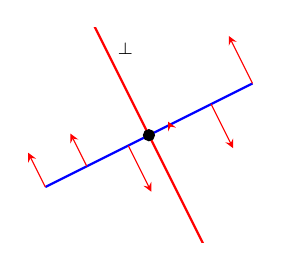
\begin{tikzpicture}%
  \begin{axis}[footnotesize,font=\footnotesize
  ,axis equal ,axis x line=none ,axis y line=none
  ,samples=6, domain=-1:1, ymax=1, ymin=-1]
  \addplot[black,mark=*]coordinates {(0,0)};
  \addplot[blue,thick] {x/2};
  \node[below] at (axis cs:1,0.5) {$\WW$};
  \addplot[red,thick] {-2*x};
  \node[right] at (axis cs:-0.4,0.8) {$\WW^\perp$};
  \addplot[red,
  quiver={u=-cos(9950*exp(x))/3,v=cos(9950*exp(x))*2/3}, 
  -stealth,update limits] {x/2};
  \end{axis}
\end{tikzpicture}}
Given the blue subspace~\WW\ in~\(\RR^2\) (the origin is a black dot), consider the set of all vectors at \idx{right-angles} to~\WW\ (drawn arrows).  Move the base of these vectors to the origin, and then they all lie in the red subspace~\(\WW^\perp\).
\vspace{2\baselineskip}
\end{figbox}


\item 
\begin{figbox}{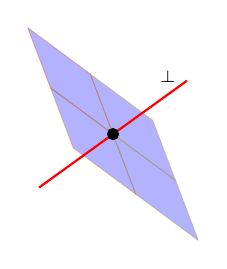
\begin{tikzpicture}%
\begin{axis}[width=15em,height=15em,scale only axis
,axis equal image,view={70}{30},font=\footnotesize
,domain=-2:2
,axis x line=none ,axis y line=none,axis z line=none]
  \addplot3[black,mark=*]coordinates {(0,0,0)};
  \addplot3[surf,blue,opacity=0.3,samples=3] {-x/2-y};
  \node[below] at (axis cs:1,0.5,-1) {$\WW$};
  \addplot3[red,thick] ({x/2},{x},{x});
  \node[left] at (axis cs:1,2,2) {$\WW^\perp$};
\end{axis}
\end{tikzpicture}}
Given the blue plane subspace~\WW\ in~\(\RR^3\) (the origin is a black dot),  the red line subspace~\(\WW^\perp\) contains all vectors orthogonal to~\WW\ (when drawn with their base at the origin).
\vspace{2.5\baselineskip}
\end{figbox}

\item 
\begin{figbox}{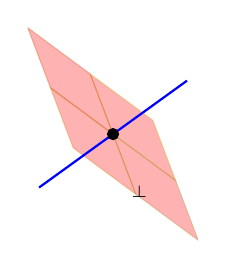
\begin{tikzpicture}%
\begin{axis}[width=15em,height=15em,scale only axis
,axis equal image,view={70}{30},font=\footnotesize
,domain=-2:2
,axis x line=none ,axis y line=none,axis z line=none]
  \addplot3[black,mark=*]coordinates {(0,0,0)};
  \addplot3[surf,red,opacity=0.3,samples=3] {-x/2-y};
  \node[below] at (axis cs:1,0.5,-1) {$\WW^\perp$};
  \addplot3[blue,thick] ({x/2},{x},{x});
  \node[left] at (axis cs:1,2,2) {$\WW$};
\end{axis}
\end{tikzpicture}}
Conversely, given the blue line subspace~\WW\ in~\(\RR^3\) (the origin is a black dot),  the red plane subspace~\(\WW^\perp\) contains all vectors orthogonal to~\WW\ (when drawn with their base at the origin).
\vspace{2.5\baselineskip}
\end{figbox}
\end{enumerate}



\begin{activity}
Given the above qualitative description of an \idx{orthogonal complement}, which of the following red lines is the \idx{orthogonal complement} to the shown (blue) \idx{subspace}~\WW?
\def\temp#1{\begin{tikzpicture}
  \begin{axis}[footnotesize,font=\footnotesize,ymin=-1.1,ymax=1.1
  ,axis equal ,axis lines=middle,samples=2, domain=-1:1]
  \addplot[blue,thick] {-x*2/3};
  \node[below] at (axis cs:1,-0.67) {$\WW$};
  \ifcase#1\addplot[red,thick] {3/2*x};
  \or\addplot[red,thick] {3/2*x+1/2};
  \or\addplot[red,thick] {2/3*x};
  \or\addplot[red,thick] {x-1/3};
  \fi
  \end{axis}
\end{tikzpicture}}
\actposs{\temp0}{\temp1}{\temp2}{\temp3}
\end{activity}




\begin{definition}[orthogonal complement] \label{def:orthsubsp}
Let \WW\ be a \(k\)-\idx{dimension}al \idx{subspace} of~\(\RR^n\).
The set of all vectors \(\uv\in\RR^n\) (together with~\ov) that are each orthogonal to all vectors in~\WW\ is called the \bfidx{orthogonal complement}~\(\WW^\perp\) (``W-\idx{perp}''); that is,
\begin{equation*}
\WW^\perp=\{\uv\in\RR^n : \uv\cdot\wv=0\text{ for all }\wv\in\WW\}.
\end{equation*}
\end{definition}


\begin{example}[\idx{orthogonal complement}] \label{eg:orthsubsp}
\ 
\begin{enumerate}[ref=\ref{eg:orthsubsp}(\alph*)]
\item\label[example]{eg:orthsubsp:a} Given the subspace \(\WW=\Span\{(3,4)\}\), find its orthogonal complement \(\WW^\perp\). 

\begin{figbox}{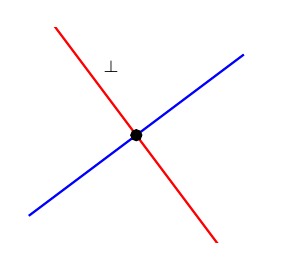
\begin{tikzpicture}
  \begin{axis}[footnotesize,font=\footnotesize
  ,axis equal,axis lines=none
  ,samples=2, domain=-1:1, ymax=1, ymin=-1]
  \addplot[black,mark=*]coordinates {(0,0)};
  \addplot[blue,thick] {x*3/4};
  \node[below] at (axis cs:1,0.75) {$\WW$};
  \addplot[red,thick] {-4/3*x};
  \node[right] at (axis cs:-0.4,0.6) {$\WW^\perp$};
  \end{axis}
\end{tikzpicture}}
\begin{solution} 
Every vector in~\WW\ is of the form \(\wv=(3c,4c)\).
For any vector \(\vv=(u,v)\in\RR^2\) the dot product 
\begin{equation*}
\wv\cdot\vv
=(3c,4c)\cdot(u,v)
=c(3u+4v).
\end{equation*}
This dot product is zero for all~\(c\) if and only if \(3u+4v=0\)\,. 
That is, when \(u=-4v/3\)\,. 
Hence \(\vv=(-\tfrac43v,v)=(-\tfrac43,1)v\), for every~\(v\), and so \(\WW^\perp=\Span\{(-\tfrac43,1)\}\).
\end{solution}
\end{figbox}


\item 
\begin{figbox}{\qview{18}{22}{\begin{tikzpicture} 
\begin{axis}[small,scale only axis
,axis equal image,font=\footnotesize
,xlabel={$v_1$},ylabel={$v_2$},zlabel={$v_3$},label shift={-2ex}
,domain=-1:1,view={\q}{25} ]
  \addplot3[black,mark=*]coordinates {(0,0,0)};
  \addplot3[surf,red,opacity=0.3,samples=3] {-x*4/7+y*4/7};
  \node[below] at (axis cs:1,-1,-1.1) {$\WW^\perp$};
  \addplot3[blue,thick] ({x},{-x},{7*x/4});
  \node[above] at (axis cs:1,-1,1.7) {$\WW$};
\end{axis}
\end{tikzpicture}}}
Describe the \idx{orthogonal complement}~\(\XX^\perp\) to the subspace \(\XX=\Span\{(4,-4,7)\}\).
\begin{solution} 
Every vector in~\WW\ is of the form \(\wv=(4,-4,7)c\).
Seek all vectors~\vv\ such that \(\wv\cdot\vv=0\)\,.  
For vectors \(\vv=(v_1,v_2,v_3)\) the dot product
\begin{align*}
\wv\cdot\vv
&=c(4,-4,7)\cdot(v_1,v_2,v_3)
\\&=c(4v_1-4v_2+7v_3)
\end{align*}
is zero for all~\(c\) if and only if \(4v_1-4v_2+7v_3=0\)\,. 
That is, the orthogonal complement is all vectors~\vv\ in the plane \(4v_1-4v_2+7v_3=0\)  (illustrated in stereo).
\end{solution}
\end{figbox}


\item Describe the \idx{orthogonal complement} of the set \(\WW=\{(t,t^2): t\in\RR\}\).
\begin{solution} 
It does not exist as an orthogonal complement is only defined for a subspace, and the parabola~\((t,t^2)\) is not a subspace.
\end{solution}



\item Given the subspace \(\WW=\Span\{(2,-2,1)\clb (2,1,-2)\}\), determine the \idx{orthogonal complement} of~\WW.
\begin{solution} 
Let \(\wv_1=(2,-2,1)\) and \(\wv_2=(2,1,-2)\) then all vectors \(\wv\in\WW\) are of the form \(\wv=c_1\wv_1+c_2\wv_2\) for all~\(c_1\) and~\(c_2\).
Every vector \(\vv\in\WW^\perp\) must satisfy, for all~\(c_1\) and~\(c_2\),
\begin{equation*}
\wv\cdot\vv=(c_1\wv_1+c_2\wv_2)\cdot\vv
=c_1\wv_1\cdot\vv+c_2\wv_2\cdot\vv
=0\,.
\end{equation*}
The only way to be zero for all~\(c_1\) and~\(c_2\) is for \emph{both} \(\wv_1\cdot\vv=0\) and \(\wv_2\cdot\vv=0\)\,.
For vectors \(\vv=(v_1,v_2,v_3)\) these two equations become the pair
\begin{eqnarray*}
2v_1-2v_2+v_3=0 \quad\text{and}\quad 2v_1+v_2-2v_3=0\,.
\end{eqnarray*}
Adding twice the second to the first, and subtracting the first from the second give the equivalent pair
\par\begin{figbox}{\qview{68}{72}{\begin{tikzpicture} 
\begin{axis}[small,font=\footnotesize,axis equal image,view={\q}{30}
,xlabel={$v_1$},ylabel={$v_2$},zlabel={$v_3$},label shift={-2ex}
,domain=-2:2,y domain=-2:2,zmax=2,zmin=-2]
    \addplot3[quiver={u=2,v=-2,w=1},blue,-stealth,thick] 
    coordinates {(0,0,0)};
    \addplot3[quiver={u=2,v=1,w=-2},blue,-stealth,thick] 
    coordinates {(0,0,0)};
    \addplot3[surf,blue,opacity=0.3,samples=3] {-x/2-y};
    \node[right] at (axis cs:-2,-1,1.5) {$\WW$};
    \addplot3[red,thick] ({x},{2*x},{2*x});
    \node[left] at (axis cs:1,2,2) {$\WW^\perp$};
\end{axis}
\end{tikzpicture}}}
\begin{equation*}
6v_1-3v_3=0\quad\text{and}\quad 3v_2-3v_3=0\,.
\end{equation*}
Both are satisfied for all \(v_3=t\) with \(v_1=t/2\) and \(v_2=t\)\,.
Therefore all possible \(\vv\)~in the complement~\(\WW^\perp\) are those in the form of the line \(\vv=(\tfrac12t,t,t)\).
That is, \(\WW^\perp=\Span\{(\tfrac12,1,1)\}\) (as illustrated in stereo).
\aqed
\end{figbox}
\end{solution}

\end{enumerate}
\end{example}



\begin{activity}
Which of the following vectors are in the \idx{orthogonal complement} of the vector space spanned by~\((3,-1,1)\)?
\actposs[4]{\((3,5,-4)\)}{\((-1,-1,1)\)}{\((1,3,-1)\)}{\((6,-2,2)\)}
\end{activity}



\begin{example} 
Prove \(\{\ov\}^\perp=\RR^n\) and \((\RR^n)^\perp=\{\ov\}\)\,.
\begin{solution} 
\begin{itemize}
\item The only vector in \(\{\ov\}\) is \(\wv=\ov\).
Since all vectors \(\vv\in\RR^n\) satisfy \(\wv\cdot\vv=\ov\cdot\vv=0\)\,, by \cref{def:orthsubsp} \(\{\ov\}^\perp=\RR^n\).

\item Certainly, \(\ov\in(\RR^n)^\perp\) as \(\wv\cdot\ov=0\) for all vectors \(\wv\in\RR^n\).
Establish there are no others by \idx{contradiction}.
Assume a nonzero vector \(\vv\in(\RR^n)^\perp\).
Now set \(\wv=\vv\in\RR^n\), then \(\wv\cdot\vv=\vv\cdot\vv=|\vv|^2\neq0\) as \(\vv\)~is nonzero.
Consequently, a nonzero~\(\vv\) cannot be in the complement.
Thus \((\RR^n)^\perp=\{\ov\}\).
\end{itemize}
\end{solution}
\end{example}




%\begin{theorem}[orthogonal complement] \label{thm:orthsubsp}
%Let \WW\ be a \(k\)-dimensional \idx{subspace} of~\(\RR^n\), 
%then \(\proj_\WW(\vv)=\ov\) for all \(\vv\in\WW^\perp\), and \(\WW^\perp\)~is a subspace of~\(\RR^n\).
%\end{theorem}
%
%\begin{proof} 
%To prove \cref{thm:orthsubsp}, recall that \cref{thm:projmat} establishes that solving \(\proj_\WW(\vv)=\ov\) for~\vv\ is identical to solving the matrix equation \((W\tr W)\vv=\ov\)\,.  
%All these solutions form the nullspace \(\Null(W\tr W)\) which is a subspace (\cref{thm:homosubsp}).
%Consequently, \(\WW^\perp\) is a subspace.
%\end{proof}
%
%
%The preceding proof used that the orthogonal complement is the nullspace of~\(W\tr W\).
%But it is often more useful to know the simpler property that the orthogonal complement is the nullspace of~\(\tr W\).

These examples find that \idx{orthogonal complement}s are lines, planes, or the entire space.  
These indicate that an orthogonal complement is generally a \idx{subspace} as proved next.

\begin{theorem}[orthogonal complement is a subspace] \label{thm:perpnull}
For every \idx{subspace}~\WW\ of~\(\RR^n\),  the \idx{orthogonal complement}~\(\WW^\perp\) is a \idx{subspace} of~\(\RR^n\).
Further, the \idx{intersection} \(\WW\cap\WW^\perp=\{\ov\}\); that is, the \idx{zero vector} is the only vector in both~\WW\ and~\(\WW^\perp\).
\end{theorem}

\begin{proof} 
Recall the \cref{def:subspace} of a subspace: we need to establish that~\(\WW^\perp\) has the zero vector, and is closed under addition and scalar multiplication.
We invoke its \cref{def:orthsubsp}.
\begin{itemize}
\item For all \(\wv\in\WW\), \(\ov\cdot\wv=0\) and so \(\ov\in\WW^\perp\).
\item Let \(\vv_1,\vv_2\in\WW^\perp\), then for all \(\wv\in\WW\) the dot product  \((\vv_1+\vv_2)\cdot\wv=\vv_1\cdot\wv+\vv_2\cdot\wv=0+0=0\) and so \(\vv_1+\vv_2\in\WW^\perp\).
\item Let scalar \(c\in\RR\) and \(\vv\in\WW^\perp\), then for all \(\wv\in\WW\) the dot product  \((c\vv)\cdot\wv=c(\vv\cdot\wv)=c0=0\) and so \(c\vv\in\WW^\perp\).
\end{itemize}
Hence, by \cref{def:subspace}, \(\WW^\perp\)~is a subspace.

Further, as they are both subspaces, the zero vector is in both~\WW\ and~\(\WW^\perp\).
Let vector~\uv\ be any vector in both~\WW\ and~\(\WW^\perp\).
As \(\uv\in\WW^\perp\), by \cref{def:orthsubsp} \(\uv\cdot\wv=0\) for all \(\wv\in\WW\).
But \(\uv\in\WW\) also, so using this for~\wv\ in the previous equation gives \(\uv\cdot\uv=0\)\,; that is, \(|\uv|^2=0\)\,.
Hence vector~\uv\ has to be the zero vector (\cref{thm:veclen0}).
That is, \(\WW\cap\WW^\perp=\{\ov\}\).
\end{proof}

\begin{activity}
Vectors in which of the following (red) sets form the \idx{orthogonal complement} to the shown (blue) \idx{subspace}~\WW?
\def\temp#1{\begin{tikzpicture}
  \begin{axis}[footnotesize,font=\footnotesize,ymin=-1.1,ymax=1.1
  ,axis equal,axis lines=middle,samples=2, domain=-1.4:1.4]
  \addplot[blue,thick] {2*x};
  \node[right] at (axis cs:0.5,1) {$\WW$};
  \ifcase#1\addplot[red,thick] {-x/2};
  \or\addplot[red,thick,samples=11,smooth] {x^2/3-x/2};
  \or\addplot[red,thick,samples=9,mark=*,only marks] {-x/2};
  \or\addplot[red,thick,mark=*,domain=-0.5:0.8] {-x/2};
  \fi
  \end{axis}
\end{tikzpicture}}
\actposs{\temp0}{\temp1}{\temp2}{\temp3}
\end{activity}


When \idx{orthogonal complement}s arise, they are often usefully written as the nullspace of a matrix.


\begin{theorem}[\idx{nullspace} complementarity] \label{thm:nulltrw}
For every \(m\times n\) matrix~\(A\), the \idx{column space} of~\(A\) has \(\Null(\tr A)\) as its \idx{orthogonal complement} in~\(\RR^m\).
That is, identifying the columns of matrix \(A=\begin{bmatrix} \av_1&\av_2&\cdots&\av_n \end{bmatrix}\), and denoting the \idx{column space} by \(\AA=\Span\{\hlist\av n\}\), then the \idx{orthogonal complement} \(\AA^\perp=\Null(\tr A)\).
Further, \(\Null(A)\) in~\(\RR^n\) is the orthogonal complement of the \idx{row space} of~\(A\).
\begin{center}
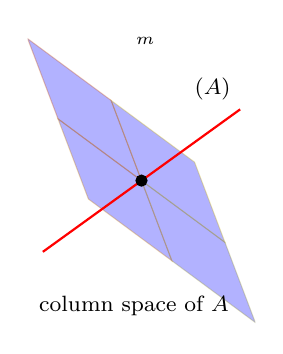
\begin{tikzpicture} 
\begin{axis}[width=20em,height=20em,scale only axis
,axis equal image,view={70}{30},font=\footnotesize
,domain=-2:2
,axis x line=none ,axis y line=none,axis z line=none]
  \addplot3[black,mark=*]coordinates {(0,0,0)};
  \node[right] at (axis cs:-1,0,3) {$\RR^m$};
  \addplot3[surf,blue,opacity=0.3,samples=3] {-x/2-y};
  \node[left] at (axis cs:2,1.6,-2.5) {column space of $A$};
  \addplot3[red,thick] ({x/2},{x},{x});
  \node[above] at (axis cs:1,2,2) {$\Null(\tr A)\qquad\ $};
\end{axis}
\end{tikzpicture}
\hfil
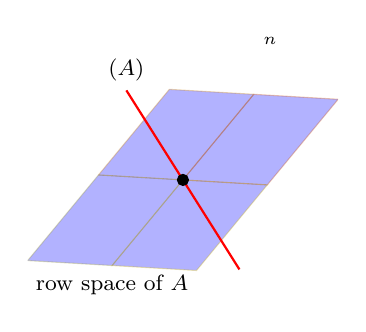
\begin{tikzpicture} 
\begin{axis}[width=15em,height=15em,scale only axis
,axis equal image,font=\footnotesize
,domain=-1:1,view={40}{25}
,axis x line=none ,axis y line=none,axis z line=none]
  \addplot3[black,mark=*]coordinates {(0,0,0)};
  \node[right] at (axis cs:0,1,1) {$\RR^n$};
  \addplot3[surf,blue,opacity=0.3,samples=3] {x/4+y/2};
  \node[below] at (axis cs:0,-1,-0.5) {row space of $A$};
  \addplot3[red,thick] ({-x/4},{-x/2},{x});
  \node[above] at (axis cs:-0.25,-0.5,1) {$\Null(A)$};
\end{axis}
\end{tikzpicture}
\end{center}
\end{theorem}

\begin{proof} 
First, by \cref{def:orthsubsp}, any vector \(\vv\in\AA^\perp\) is orthogonal to all vectors in the column space of~\(A\), in particular it is orthogonal to the columns of~\(A\):
\begin{align*}
& \av_1\cdot\vv=0,\ \av_2\cdot\vv=0,\ \ldots,\ \av_k\cdot\vv=0
\\&\iff \tr\av_1\vv=0,\ \tr\av_2\vv=0,\ \ldots,\ \tr\av_k\vv=0
\\&\iff\begin{bmatrix} \tr\av_1\\\tr\av_2\\\vdots\\\tr\av_k \end{bmatrix}\vv=\ov
\\&\iff \tr A\vv=\ov
\\&\iff\vv\in\Null(\tr A).
\end{align*}
That is, \(\AA^\perp\subseteq\Null(\tr A)\).
Second, for any \(\vv\in\Null(\tr A)\),
recall that by \cref{def:colsp} for any vector~\(\wv\) in the column space of~\(A\), there exists a linear combination \(\wv=\lincomb c\av n\). 
Then
\begin{align*}
\wv\cdot\vv&=(\lincomb c\av n)\cdot\vv
\\&=c_1(\av_1\cdot\vv)+c_2(\av_2\cdot\vv)+\cdots+c_n(\av_n\cdot\vv)
\\&=c_10+c_20+\cdots+c_n0
\quad(\text{from above}\iff)
\\&=0\,,
\end{align*}
and so by \cref{def:orthsubsp} vector \(\vv\in\AA^\perp\); that is, \(\Null(\tr A)\subseteq\AA^\perp\).
Putting these two together, \(\Null(\tr A)=\AA^\perp\).

Lastly, that the \(\Null(A)\) in~\(\RR^n\) is the orthogonal complement of the \idx{row space} of~\(A\) follows from applying the above result to the matrix~\(\tr A\).
\end{proof}



\begin{example} \label{eg:nulltrw}
\ 
\begin{enumerate}[ref=\ref{eg:nulltrw}(\alph*)]
\item\label[example]{eg:nulltrw:a} Let the subspace \(\WW=\Span\{(2,-1)\}\). Find the \idx{orthogonal complement}~\(\WW^\perp\). 

\begin{figbox}{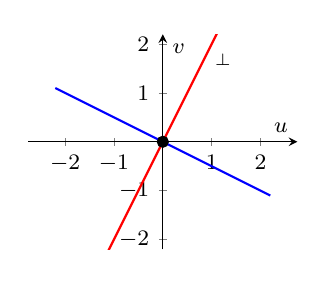
\begin{tikzpicture}
  \begin{axis}[footnotesize,font=\footnotesize
  ,axis equal ,axis lines=middle ,xlabel={$u$},ylabel={$v$}
  ,samples=2, domain=-2.2:2.2, ymax=2.2, ymin=-2.2]
  \addplot[black,mark=*]coordinates {(0,0)};
  \addplot[blue,thick] {-x/2};
  \node[below] at (axis cs:2,-1) {$\WW$};
  \addplot[red,thick] {2*x};
  \node[below] at (axis cs:1,2) {\quad$\WW^\perp$};
  \end{axis}
\end{tikzpicture}}
\begin{solution} 
Here the subspace~\WW\ is the column space of the matrix \(W=\begin{bmat} 2\\-1 \end{bmat}\).
To find \(\WW^\perp=\Null(\tr W)\), solve \(\tr W\vv=\ov\)\,, that is, for vectors \(\vv=(u,v)\)
\begin{equation*}
\begin{bmatrix} 2&-1 \end{bmatrix}\vv=2u-v=0\,.
\end{equation*}
All solutions are \(v=2u\) (as illustrated).
Hence \(\vv=(u,2u)=(1,2)u\), and so \(\WW^\perp=\Span\{(1,2)\}\).
\end{solution}
\end{figbox}


\item\label[example]{eg:nulltrw:b} Describe the subspace of~\(\RR^3\) whose \idx{orthogonal complement} is the plane \(-\tfrac12x-y+2z=0\)\,. 

\begin{figbox}{\qview{38}{42}{\begin{tikzpicture} 
\begin{axis}[footnotesize,scale only axis
,xlabel={$x$},ylabel={$y$},zlabel={$z$},label shift={-2ex}
,axis equal image,font=\footnotesize
,domain=-1:1,view={\q}{25}
]
  \addplot3[black,mark=*]coordinates {(0,0,0)};
  \addplot3[surf,red,opacity=0.3,samples=3] {x/4+y/2};
  \node[below] at (axis cs:0,-1,-0.5) {$\WW^\perp$};
  \addplot3[blue,thick] ({-x/4},{-x/2},{x});
  \node[above] at (axis cs:-0.25,-0.5,1) {$\WW$};
\end{axis}
\end{tikzpicture}}}
\begin{solution} 
The equation of the plane in \(\RR^3\) may be written 
\begin{equation*}
\begin{bmatrix} -\tfrac12&-1&2 \end{bmatrix}
\begin{bmatrix} x\\y\\z \end{bmatrix}=0\,,
\end{equation*}
that is  \(\tr W\vv=0\)
for matrix \(W=\begin{bmatrix} \wv_1 \end{bmatrix}\) and vectors \(\wv_1=(-\tfrac12,-1,2)\) and \(\vv=(x,y,z)\).
Since the plane is the nullspace of matrix~\(\tr W\), the plane must be the orthogonal complement of the line \(\WW=\Span\{\wv_1\}\) (as illustrated below).
\end{solution}
\end{figbox}


\item\label[example]{eg:nulltrw:c} Find the \idx{orthogonal complement} to the \idx{column space} of matrix
\begin{equation*}
A=\begin{bmatrix} 1&-1&0\\ 1&0&-1\\ 0&1&-1 \end{bmatrix}.
\end{equation*}
\begin{solution} 
The required orthogonal complement is the nullspace of~\(\tr A\).
Recall from \cref{sec:isle} that for such small problems we find all solutions of \(\tr A\vv=\ov\) by algebraic elimination; that is,
\begin{eqnarray*}
\begin{bmatrix} 1&1&0\\-1&0&1\\ 0&-1&-1 \end{bmatrix}\vv=\ov
&\iff&
\begin{cases}
v_1+v_2=0\,,\\
-v_1+v_3=0\,,\\
-v_2-v_3=0\,,
\end{cases}
\\&\iff&\begin{cases}
v_2=-v_1\,,\\
v_3=v_1\,,\\
-v_2-v_3=v_1-v_1=0\,.
\end{cases}
\end{eqnarray*}
Therefore all solutions of \(\tr A\vv=\ov\) are of the form \(v_1=t\)\,, \(v_2=-v_1=-t\) and \(v_3=v_1=t\); that is, \(\vv=(1,-1,1)t\).
Hence the orthogonal complement is \(\Span\{(1,-1,1)\}\).
\end{solution}

\item\label[example]{eg:nulltrw:d} Describe the \idx{orthogonal complement} of the subspace spanned by the four vectors \((1,1,0,1,0,0)\), \((-1,0,1,0,1,0)\), \((0,-1,-1,0,0,1)\) and \((0,0,0,-1,-1,-1)\).
\begin{solution} 
Arrange these vectors as the four columns of a matrix, say
\setbox\ajrqrbox\hbox{\qrcode{% orth comp
A=[1  -1   0   0
   1   0  -1   0
   0   1  -1   0
   1   0   0  -1
   0   1   0  -1
   0   0   1  -1 ]
[U,S,V]=svd(A)
}}%
\marginajrbox%
\begin{equation*}
A=\begin{bmatrix}    1 & -1 & 0 & 0
\\ 1 & 0 & -1 & 0
\\ 0 & 1 & -1 & 0
\\ 1 & 0 & 0 & -1
\\ 0 & 1 & 0 & -1
\\ 0 & 0 & 1 & -1
 \end{bmatrix},
\end{equation*}
then seek \(\Null(\tr A)\), the solutions of \(\tr A\xv=\ov\).
Adapt \cref{pro:gensol} to solve \(\tr A\xv=\ov\)\,:
\begin{enumerate}
\item \cref{eg:roundrobin1} computed an \svd\ \(A=\usv\) for this matrix~\(A\), which gives the \svd\ \(\tr A=V\tr S\tr U\) for the transpose where \twodp
\begin{verbatim}
U =
  0.31 -0.26 -0.58 -0.26  0.64 -0.15
  0.07  0.40 -0.58  0.06 -0.49 -0.51
 -0.24  0.67  0.00 -0.64  0.19  0.24
 -0.38 -0.14 -0.58  0.21 -0.15  0.66
 -0.70  0.13  0.00  0.37  0.45 -0.40
 -0.46 -0.54 -0.00 -0.58 -0.30 -0.26
S =
  2.00     0     0     0
     0  2.00     0     0
     0     0  2.00     0
     0     0     0  0.00
     0     0     0     0
     0     0     0     0
V = ...
\end{verbatim}

\item \(V\zv=\ov\) determines \(\zv=\ov\)\,.
\item \(\tr S\yv=\zv=\ov\) determines \(y_1=y_2=y_3=0\) as there are three nonzero singular values, and \(y_4\), \(y_5\) and~\(y_6\) are free variables; that is, \(\yv=(0,0,0,y_4,y_5,y_6)\).
\item Denoting the columns of~\(U\) by \hlist\uv 6, the solutions of \(\tr U\xv=\yv\) are \(\xv=U\yv=\uv_4y_4+\uv_5y_5+\uv_6y_6\).
\end{enumerate}
That is, the orthogonal complement is the three dimensional subspace \(\Span\{\uv_4,\uv_5,\uv_6\}\) in~\(\RR^6\),  where \twodp\
\begin{eqnarray*}
&&\uv_4=(-0.26,0.06,-0.64,0.21,0.37,-0.58),
\\&&\uv_5=(0.64,-0.49,0.19,-0.15,0.45,-0.30), 
\\&&\uv_6=(-0.15,-0.51,0.24,0.66,-0.40,-0.26).
\end{eqnarray*}
\end{solution}

\end{enumerate}
\end{example}


In the previous \cref{eg:nulltrw:d} there are three nonzero \idx{singular value}s in the first three rows of~\(S\).
These three nonzero singular values determine that the first three columns of~\(U\) form a basis for the \idx{column space} of~\(A\).
The example argues that the remaining three columns of~\(U\) form a basis for the \idx{orthogonal complement} of the column space.
That is, all six of the columns of the orthogonal~\(U\) are used in either the column space or its complement.
This is \text{generally true.}

\begin{activity}
A given matrix~\(A\) has \idx{column space}~\WW\ such that \(\dim\WW=4\) and \(\dim\WW^\perp=3\)\,.  
What \idx{size} could the matrix be?
\actposs[4]{\(7\times5\)}{\(3\times4\)}{\(4\times3\)}{\(7\times3\)}
\end{activity}



\begin{example} \label{eg:orthrank}
Recall the cases of \cref{eg:nulltrw}.
\begin{description}
\item[\ref{eg:nulltrw:a}] \(\dim\WW+\dim\WW^\perp=1+1=2=\dim\RR^2\).
\item[\ref{eg:nulltrw:b}] \(\dim\WW+\dim\WW^\perp=1+2=3=\dim\RR^3\).
\item[\ref{eg:nulltrw:c}] \(\dim\WW+\dim\WW^\perp=2+1=3=\dim\RR^3\).
\item[\ref{eg:nulltrw:d}] \(\dim\WW+\dim\WW^\perp=3+3=6=\dim\RR^6\).
\end{description}
\end{example}

Recall the Rank \cref{thm:rank} connects the  dimension of a space with the dimensions of a \idx{nullspace} and \idx{column space} of a matrix.
Since a \idx{subspace} is closely connected to matrices, and its orthogonal complement is connected to nullspaces, then the Rank Theorem should say something \text{general here.}



\begin{theorem} \label{thm:orthrank}
Let \WW\ be a \idx{subspace} of~\(\RR^n\), then \(\dim\WW+\dim\WW^\perp=n\)\,; equivalently, \(\dim\WW^\perp=n-\dim\WW\).
\end{theorem}

\begin{proof} 
Let the columns of a matrix~\(W\) form an orthonormal basis for the subspace~\WW\ (\cref{thm:obaseexists} asserts a basis exists).
\cref{thm:nulltrw} establishes that \(\WW^\perp=\Null(\tr W)\).
Equating dimensions of both sides, 
\begin{eqnarray*}
\dim\WW^\perp&=&\nullity(\tr W) 
\quad(\text{from \cref{def:nullity}})
\\&=&n-\rank(\tr W)
\quad(\text{from Rank \cref{thm:rank}})
\\&=&n-\rank(W)
\quad(\text{from \cref{thm:ranktr}})
\\&=&n-\dim\WW
\quad(\text{from \cref{pro:ospan}}),
\end{eqnarray*}
as required.
\end{proof}


Since the \idx{dimension} of the whole space is the sum of the dimension of a \idx{subspace} plus the dimension of its \idx{orthogonal complement}, surely we must be able to separate vectors into two corresponding \idx{components}.

\begin{example} \label{eg:perp2}
Recall from \cref{eg:orthsubsp:a} that subspace \(\WW=\Span\{(3,4)\}\) has \idx{orthogonal complement} \(\WW^\perp=\Span\{(-4,3)\}\), as illustrated.

\begin{figbox}{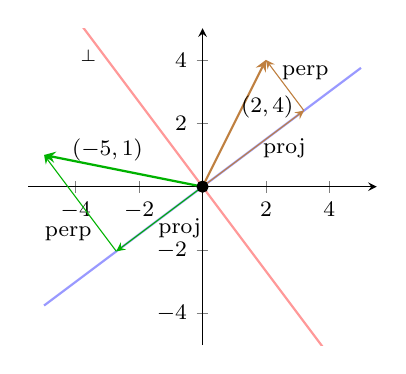
\begin{tikzpicture}%
[baseline={([yshift={-\ht\strutbox}]current bounding box.north)}]
  \begin{axis}[small,font=\footnotesize
  ,axis equal image,axis lines=middle
  ,samples=2, domain=-5:5, xmin=-5.5, xmax=5.5, ymax=5, ymin=-5]
  \addplot[black,mark=*]coordinates {(0,0)};
  \addplot[blue,thick,opacity=0.4] {x*3/4};
  \node[right] at (axis cs:4,3) {$\WW$};
  \addplot[red,thick,opacity=0.4] {-4/3*x};
  \node[left] at (axis cs:-3,4) {$\WW^\perp$};
  %
  \addplot[brown,-stealth,quiver={u=2,v=4},thick] coordinates {(0,0)};
  \addplot[brown,-stealth,quiver={u=16/5,v=12/5}] coordinates {(0,0)};
  \addplot[brown,-stealth,quiver={u=-6/5,v=8/5}] coordinates {(16/5,12/5)};
  \node[] at (axis cs:1.3,2.5) {\qquad $(2,4)$};
  \node[right] at (axis cs:1.6,1.2) {proj};
  \node[right] at (axis cs:2.2,3.6) {perp};
  %
  \addplot[green!70!black,-stealth,quiver={u=-5,v=1},thick] coordinates {(0,0)};
  \addplot[green!70!black,-stealth,quiver={u=-2.72,v=-2.04}] coordinates {(0,0)};
  \addplot[green!70!black,-stealth,quiver={u=-2.28,v=3.04}] coordinates {(-2.72,-2.04)};
  \node[above] at (axis cs:-3,0.5) {$(-5,1)$};
  \node[right] at (axis cs:-1.7,-1.3) {proj};
  \node[left] at (axis cs:-3.2,-1.5) {perp};
  \end{axis}
\end{tikzpicture}}
As shown, for example,  write the brown vector \((2,4)=(3.2,2.4)+(-1.2,1.6)=\proj_\WW(2,4)+\Perp\), where here the vector \(\Perp=(-1.2,1.6)\in\WW^\perp\).
Indeed, any vector can be written as a component in subspace~\WW\ and a component in the orthogonal complement~\(\WW^\perp\) (\cref{thm:odt}).
\quad For another example,  write the green vector \((-5,1)=(-2.72,-2.04)+(-2.28,3.04)=\proj_\WW(-5,1)+\Perp\), where in this case the vector \(\Perp=(-2.28,3.04)\in\WW^\perp\).
\aqed
\end{figbox}
\end{example}



\begin{activity}
Let \idx{subspace} \(\WW=\Span\{(1,1)\}\) and its \idx{orthogonal complement} \(\WW^\perp=\Span\{(1,-1)\}\).  
Which of the following writes vector \((5,-9)\) as a sum of two vectors, one from each of~\WW\ and~\(\WW^\perp\)?
\actposs{\((-2,-2)+(7,-7)\)}
{\((5,5)+(0,-14)\)}
{\((7,7)+(-2,2)\)}
{\((9,-9)+(-4,0)\)}
\end{activity}




Further, such a separation can be done for any pair of complementary \idx{subspace}s~\WW\ and~\(\WW^\perp\) within any space~\(\RR^n\).
To proceed, let's define what is meant by ``\Perp'' in such a context.


\begin{definition}[perpendicular component] \label{def:perpn}
Let \WW\ be a \idx{subspace} of~\(\RR^n\).
For every vector \(\vv\in\RR^n\), the \bfidx{perpendicular component} of~\vv\  to~\WW\ is the vector
\(\Perp_\WW(\vv):=\vv-\proj_{\WW}(\vv)\).
\end{definition}

%From \cref{thm:nulltrw} we know the orthogonal complement~\(\WW^\perp\) is the \idx{nullspace} of~\(\tr W\) for matrix~\(W\) whose columns are an orthonormal basis for~\WW.
%The following examples use this to find \(\Perp_\WW(\vv)\). 



\begin{example} \label{eg:perpn}
\begin{enumerate}[ref=\ref{eg:perpn}(\alph*)]
\item\label[example]{eg:perpn:a} Let the subspace~\WW\ be the span of \((-2,-3,6)\).  
Find the \idx{perpendicular component} to~\WW\ of the vector \((4,1,3)\).
Verify the perpendicular component lies in the plane \(-2x-3y+6z=0\)\,.
\begin{solution} 
Projection is easiest with a unit vector.
Obtain a unit vector to span~\WW\ by normalizing the basis vector to \(\wv_1=(-2,-3,6)/\sqrt{2^2+3^2+6^2}=(-2,-3,6)/7\)\,.
Then
\begin{eqnarray*}
\Perp_\WW(4,1,3)&=&(4,1,3)-\wv_1(\wv_1\cdot(4,1,3))
\\&=&(4,1,3)-\wv_1(-8-3+18)/7
\\&=&(4,1,3)-\wv_1=(30,10,15)/7\,.
\end{eqnarray*}
\begin{figbox}{\qview{48}{52}{\begin{tikzpicture} 
\begin{axis}[small,axis equal image,font=\footnotesize
,xlabel={$x$},ylabel={$y$},zlabel={$z$},label shift={-2ex}
,domain=-5:5,view={\q}{25} ]
  \addplot3[black,mark=*]coordinates {(0,0,0)};
  \addplot3[surf,red,opacity=0.2,samples=3] {x*2/6+y*3/6};
  \node[below] at (axis cs:5,-5,0) {$\WW^\perp$};
  \addplot3[blue,thick] ({-x*2/6},{-x*3/6},{x});
  \node[above] at (axis cs:-1.66,-2.5,5) {$\WW$};
  \addplot3[quiver={u=4,v=1,w=3},brown,-stealth,thick] coordinates {(0,0,0)};
  \node[above,font=\tiny] at (axis cs:4,1,3) {$(4,1,3)$};
  \addplot3[quiver={u=30/7,v=10/7,w=15/7},brown,-stealth,thick] coordinates {(0,0,0)};
  \addplot3[quiver={u=-2/7,v=-3/7,w=6/7},brown] coordinates {(30/7,10/7,15/7)};
  \node[below,font=\tiny] at (axis cs:4.29,1.43,2.14) {perp};%{$(\frac{30}7,\frac{10}7,\frac{15}7)$};
\end{axis}
\end{tikzpicture}}}
For \((x,y,z)=(30,10,15)/7\) we find
\begin{align*}
-2x-3y+6z&=\tfrac17(-60-30+90)\\&=\tfrac170=0\,.
\end{align*}
Hence \(\Perp_\WW(4,1,3)\) lies in the plane \(-2x-3y+6z=0\) (which is the orthogonal complement~\(\WW^\perp\), as illustrated in stereo to the right).
\aqed

\end{figbox}
\end{solution}


\item\label[example]{eg:perpn:b} For the vector \((-5,-1,6)\) find its \idx{perpendicular component} to the subspace~\WW\ spanned by~\((-2,-3,6)\).
Verify the perpendicular component lies in the plane \(-2x-3y+6z=0\)\,.
\begin{solution} 
As in the previous case, use the basis vector \(\wv_1=(-2,-3,6)/7\)\,.
Then
\begin{eqnarray*}
\Perp_\WW(-5,-1,6)&=&(-5,-1,6)-\wv_1(\wv_1\cdot(-5,-1,6))
\\&=&(-5,-1,6)-\wv_1(10+3+36)/7
\\&=&(-5,-1,6)-\wv_17=(-3,2,0).
\end{eqnarray*}

\begin{figbox}{\qview{8}{12}{\begin{tikzpicture} 
\begin{axis}[small,axis equal image,font=\footnotesize
,xlabel={$x$},ylabel={$y$},zlabel={$z$},label shift={-2ex}
,domain=-5:5,view={\q}{20} ]
  \addplot3[black,mark=*]coordinates {(0,0,0)};
  \addplot3[surf,red,opacity=0.2,samples=3] {x*2/6+y*3/6};
  \node[below] at (axis cs:5,-5,0) {$\WW^\perp$};
  \addplot3[blue,thick] ({-x*2/6},{-x*3/6},{x});
  \node[below] at (axis cs:+1.66,+2.5,-5) {$\WW$};
  \addplot3[quiver={u=-5,v=-1,w=6},brown,-stealth,thick] coordinates {(0,0,0)};
  \node[right,font=\tiny] at (axis cs:-5,-1,6) {$(-5,-1,6)$};
  \addplot3[quiver={u=-3,v=2,w=0},brown,-stealth,thick] coordinates {(0,0,0)};
  \addplot3[quiver={u=-2,v=-3,w=6},brown] coordinates {(-3,2,0)};
  \node[below,font=\tiny] at (axis cs:-3,2,0) {perp};%{$(-3,2,0)$};
\end{axis}
\end{tikzpicture}}}
For \((x,y,z)=(-3,2,0)\) we find \(-2x-3y+6z=6-6+0=0\)\,.
Hence \(\Perp_\WW(-5,-1,6)\) lies in the plane \(-2x-3y+6z=0\) (which is the orthogonal complement~\(\WW^\perp\), as illustrated to the right in stereo).
\aqed
\end{figbox}
\end{solution}

\item\label[example]{eg:perpn:c} Let the subspace \(\XX=\Span\{(2,-2,1)\clb (2,1,-2)\}\).
Determine the \idx{perpendicular component} of each of the two vectors \(\yv=(3,2,1)\) and \(\zv=(3,-3,-3)\).
\begin{solution} 
Computing \(\proj_\XX\) needs an orthonormal basis for~\XX\ (\cref{def:orthproj}).
The two vectors in the span are orthogonal, so normalize them to \(\wv_1=(2,-2,1)/3\) and \(\wv_2=(2,1,-2)/3\).
\begin{itemize}
\item Then for the first vector \(\yv=(3,2,1)\) (illustrated below in brown),
\begin{eqnarray*}
\Perp_\XX(\yv)
&=&\yv-\proj_\XX(\yv)
\\&=&\yv-\wv_1(\wv_1\cdot\yv)-\wv_2(\wv_2\cdot\yv)
\\&=&\yv-\wv_1(6-4+1)/3-\wv_2(6+2-2)/3
\\&=&\yv-\wv_1-2\wv_2
\\&=&(3,2,1)-(2,-2,1)/3-(4,2,-4)/3
\\&=&(1,2,2)
\end{eqnarray*}
\begin{center}
\qview{63}{67}{\begin{tikzpicture} 
\begin{axis}[small,font=\footnotesize,view={\q}{30},axis equal image
,xlabel={$x_1$},ylabel={$x_2$},zlabel={$x_3$},label shift={-2ex}
,domain=-3:3,y domain=-3:3,zmax=3,zmin=-3]
  \addplot3[quiver={u=2,v=-2,w=1},blue,-stealth] coordinates {(0,0,0)};
  \addplot3[quiver={u=2,v=1,w=-2},blue,-stealth] coordinates {(0,0,0)};
  \addplot3[surf,blue,opacity=0.3,samples=3] {-x/2-y};
  \node[left] at (axis cs:0,-2.5,2) {$\XX$};
  \addplot3[red,thick,opacity=0.2] ({x/2},{x},{x});
%
  \addplot3[quiver={u=3,v=2,w=1},brown,-stealth,thick] coordinates {(0,0,0)};
  \node[below] at (axis cs:3,2,1) {$\yv$};
  \addplot3[quiver={u=2,v=0,w=-1},brown] coordinates {(1,2,2)};
  \addplot3[quiver={u=1,v=2,w=2},brown,-stealth,thick] coordinates {(0,0,0)};
  \node[above] at (axis cs:1,2,2) {perp};%{$(1,2,2)$\hspace*{1em}};
%
  \addplot3[quiver={u=3,v=-3,w=-3},green!70!black,-stealth,thick] coordinates {(0,0,0)};
  \node[above] at (axis cs:3,-3,-3) {\quad$\zv$};
  \addplot3[quiver={u=4,v=-1,w=-1},green!70!black] coordinates {(-1,-2,-2)};
  \addplot3[quiver={u=-1,v=-2,w=-2},green!70!black,-stealth,thick] coordinates {(0,0,0)};
  \node[above] at (axis cs:-1,-2,-2) {perp\hspace*{1em}};
\end{axis}
\end{tikzpicture}}
\end{center}


\item For the second vector \(\zv=(3,-3,-3)\) (green in the picture above),
\begin{eqnarray*}
\Perp_\XX(\zv)
&=&\zv-\proj_\XX(\zv)
\\&=&\zv-\wv_1(\wv_1\cdot\zv)-\wv_2(\wv_2\cdot\zv)
\\&=&\zv-\wv_1(6+6-3)/3-\wv_2(6-3+6)/3
\\&=&\zv-3\wv_1-3\wv_2
\\&=&(3,-3,-3)-(2,-2,1)-(2,1,-2)
\\&=&(-1,-2,-2).
\end{eqnarray*}
\aqed
\end{itemize}
\end{solution}

\end{enumerate}
\end{example}


As seen in all these examples, the \idx{perpendicular component} of a vector always lies in the orthogonal complement to the \idx{subspace}  (as suggested by the naming).


\begin{theorem}[perpendicular component is orthogonal] \label{thm:perpn}
Let \WW\ be a \idx{subspace} of~\(\RR^n\) and let \(\vv\)~be any vector in~\(\RR^n\), then the \idx{perpendicular component} \(\Perp_\WW(\vv)\in\WW^\perp\).
\end{theorem}

\begin{proof} 
Let vectors \hlist\wv k\ form an orthonormal basis for the subspace~\WW\ (a basis exists by \cref{thm:obaseexists}).
Let the \(n\times k\) matrix \(W=\begin{bmatrix} \wv_1&\wv_2&\cdots&\wv_k \end{bmatrix}\) so subspace~\WW\ is the column space of matrix~\(W\), then \cref{thm:nulltrw} asserts we just need to check that \(\tr W\Perp_\WW(\vv)=\ov\)\,.
Consider 
\begin{eqnarray*}
\tr W\Perp_\WW(\vv)
&=&\tr W\left[\vv-\proj_\WW(\vv)\right]
\quad(\text{from \cref{def:perpn}})
\\&=&\tr W\left[\vv-(W\tr W)\vv\right]
\quad(\text{from \cref{thm:projmat}})
\\&=&\tr W\vv-\tr W(W\tr W)\vv
\quad(\text{by distributivity})
\\&=&\tr W\vv-(\tr WW)\tr W\vv 
\quad(\text{by associativity})
\\&=&\tr W\vv-I_k\tr W\vv 
\quad(\text{only if }\tr WW=I_k)
\\&=&\tr W\vv-\tr W\vv =\ov\,.
\end{eqnarray*}
Hence \(\Perp_\WW(\vv)\in\Null(\tr W)\) and so is in~\(\WW^\perp\) (by \cref{thm:nulltrw}).

But this proof only holds if \(\tr WW=I_k\)\,.
To establish this identity, use the same argument as in the proof of \cref{thm:orthog:0}$\iff$\ref{thm:orthog:ii}:
\begin{eqnarray*}
\tr WW
&=&\begin{bmatrix} \tr\wv_1\\\tr\wv_2\\\vdots\\\tr\wv_k \end{bmatrix}
\begin{bmatrix} \wv_1&\wv_2&\cdots&\wv_k \end{bmatrix}
=\begin{bmatrix} \tr\wv_1\wv_1&\tr\wv_1\wv_2&\cdots&\tr\wv_1\wv_k 
\\ \tr\wv_2\wv_1&\tr\wv_2\wv_2&\cdots&\tr\wv_2\wv_k 
\\\vdots&\vdots&\ddots&\vdots
\\ \tr\wv_k\wv_1&\tr\wv_k\wv_2&\cdots&\tr\wv_k\wv_k \end{bmatrix}
\\&=&\begin{bmatrix} \wv_1\cdot\wv_1&\wv_1\cdot\wv_2&\cdots&\wv_1\cdot\wv_k 
\\ \wv_2\cdot\wv_1&\wv_2\cdot\wv_2&\cdots&\wv_2\cdot\wv_k 
\\\vdots&\vdots&\ddots&\vdots
\\ \wv_k\cdot\wv_1&\wv_k\cdot\wv_2&\cdots&\wv_k\cdot\wv_k \end{bmatrix}
=I_k
\end{eqnarray*}
as vectors \hlist\wv k\ are an orthonormal set (from \cref{def:orthoset}, the dot product \(\wv_i\cdot\wv_j=0\) for \(i\neq j\) and \(|\wv_i|^2=\wv_i\cdot\wv_i=1\)).
%First show \(\Perp_\WW(\vv)\) is orthogonal to each basis vector.
%Let \(\wv_j\)~be any of the \(k\)~vectors in the orthonormal basis, then the dot product
%\begin{eqnarray*}
%&&\wv_j\cdot\Perp_\WW(\vv)
%\\&=&\wv_j\cdot\left[\vv-\proj_{\WW}(\vv)\right]
%\\&=&\wv_j\cdot\left[\vv-\wv_1(\wv_1\cdot\vv)-\cdots-\wv_k(\wv_k\cdot\vv)\right]
%\\&=&\wv_j\cdot\vv-(\wv_j\cdot\wv_1)(\wv_1\cdot\vv)-\cdots-(\wv_j\cdot\wv_k)(\wv_k\cdot\vv).
%\end{eqnarray*}
%By orthogonality of the basis vectors, almost all the dot products \(\wv_j\cdot\wv_1,\ldots,\wv_j\cdot\wv_k\) are zero; the exception is \(\wv_j\cdot\wv_j=|\wv_j|^2=1\) as they are unit vectors.
%Hence the dot product
%\begin{eqnarray*}
%&&\wv_j\cdot\Perp_\WW(\vv)
%\\&=&\wv_j\cdot\vv-0(\wv_1\cdot\vv)-\cdots-1(\wv_j\cdot\vv)-\cdots-0(\wv_k\cdot\vv)
%\\&=&\wv_j\cdot\vv-(\wv_j\cdot\vv)
%\\&=&0\,.
%\end{eqnarray*}
%Because the dot products are zero for all~\(j\), \(\Perp_\WW(\vv)\) is orthogonal to all the vectors \hlist\wv k\,.
%
%Second, consider any vector \(\wv\in\WW\)\,: it must be a linear combination of the orthonormal basis vectors, say
%\begin{equation*}
%\wv=\lincomb c\wv k\,,
%\end{equation*}
%for some coefficients \hlist ck.
%Then the dot product
%\begin{eqnarray*}
%&&\wv\cdot\Perp_\WW(\vv)
%\\&=&(\lincomb c\wv k)\cdot\Perp_\WW(\vv)
%\\&=&c_1\wv_1\cdot\Perp_\WW(\vv)
%+c_2\wv_2\cdot\Perp_\WW(\vv)
%+\cdots+c_k\wv_k\cdot\Perp_\WW(\vv)
%\\&=&c_10+c_20+\cdots+c_k0
%\\&=&0\,.
%\end{eqnarray*}
%Because the dot product is zero for all~\(\wv\in\WW\), \(\Perp_\WW(\vv)\) lies in~\(\WW^\perp\) (\cref{def:orthsubsp}).
\end{proof}


\begin{example} 
The previous examples' calculation of the \idx{perpendicular component} confirm that \(\vv=\proj_\WW(\vv)+\Perp_\WW(\vv)\), where we now know that \(\Perp_\WW\) is orthogonal to~\WW:
\begin{description}
\item[\cref{eg:perp2}] \((2,4)=(3.2,2.4)+(-1.2,1.6)\) and 
\\\((-5,1)=(-2.72,-2.04)+(-2.28,3.04)\);
\item[\cref{eg:perpn:b}] \((-5,-1,6)=(-2,-3,6)+(-3,2,0)\);
\item[\cref{eg:perpn:c}] \((3,2,1)=(2,0,-1)+(1,2,2)\) and 
\\\((3,-3,-3)=(4,-1,-1)+(-1,-2,-2)\).
\end{description}
\end{example}

Given any \idx{subspace}~\WW, this theorem indicates that every vector can be written as a sum of two vectors: one in the subspace~\WW; and one in its \idx{orthogonal complement}~\(\WW^\perp\).


\begin{theorem}[orthogonal decomposition] \label{thm:odt}
Let \WW\ be a \idx{subspace} of~\(\RR^n\) and vector \(\vv\in\RR^n\), then there exist unique vectors \(\wv\in\WW\) and \(\nv\in\WW^\perp\) such that vector \(\vv=\wv+\nv\)\,; this particular sum is called an \bfidx{orthogonal decomposition} of~\vv.
\end{theorem}

\begin{proof} 
First establish existence.  
By \cref{def:perpn}, \(\Perp_\WW(\vv)=\vv-\proj_\WW(\vv)\), so it follows that \(\vv=\proj_\WW(\vv)+\Perp_\WW(\vv)=\wv+\nv\) when we set \(\wv=\proj_\WW(\vv)\in\WW\) and \(\nv=\Perp_\WW(\vv)\in\WW^\perp\).

 Second establish uniqueness by \idx{contradiction}.
Suppose there is another decomposition \(\vv=\wv'+\nv'\) where \(\wv'\in\WW\) and \(\nv'\in\WW^\perp\).
Then \(\wv+\nv=\vv=\wv'+\nv'\).
Rearranging gives \(\wv-\wv'=\nv'-\nv\)\,.
By closure of a subspace under vector addition (\cref{def:subspace}), the left-hand side is in~\WW\ and the right-hand side is in~\(\WW^\perp\), so the two sides must be both in~\WW\ and~\(\WW^\perp\).
The zero vector is the only common vector to the two subspaces (\cref{thm:perpnull}), so \(\wv-\wv'=\nv'-\nv=\ov\)\,, and hence both \(\wv=\wv'\) and \(\nv=\nv'\).
That is, the decomposition must \text{be unique.}
\end{proof}


\end{reduce}
\newcommand{\projxv}[9]{\begin{tikzpicture}
  \begin{axis}[footnotesize
  ,axis equal ,axis x line=none , axis y line=none
  ,samples=2 ]
  \addplot[black,mark=*]coordinates {(0,0)};
  \addplot[red,quiver={u=#1,v=#2},-stealth]coordinates {(0,0)};
  \node[right] at (axis cs:#1,#2) {$\vec #9$};
  \addplot[blue,quiver={u=#3,v=#4},-stealth]coordinates {(0,0)};
  \node[right] at (axis cs:#3,#4) {$\vec #8$};
  \ifnum#7>0
  \addplot[black] coordinates {(#5/2,#6/2)} node {proj};
  \addplot[brown,thick,quiver={u=#5,v=#6},-stealth]coordinates {(0,0)};
  \addplot[black] coordinates {(#1/2+#5/2,#2/2+#6/2)} node {perp};
  \addplot[brown,thick,quiver={u=#1-#5,v=#2-#6},-stealth]coordinates {(#5,#6)};
  \fi
  \end{axis}
\end{tikzpicture}}
\begin{reduce}
\begin{example} 
For each pair of the shown subspaces \(\XX=\Span\{\xv\}\) and  vectors~\vv, draw the decomposition of vector~\vv\ into the sum of vectors in~\XX\ and~\(\XX^\perp\).
\begin{Parts}
\item \projxv{-0.8}{-1.6}{-1.7}{-1.3}{ -1.2769}{-0.97642}0xv
\item \projxv{-0.8}{ 1.1}{ 0.9}{-0.3}{-1.05}{ 0.35}0xv
\end{Parts}
\begin{solution} 
In each case, the two brown vectors shown are the decomposition, with \(\text{proj}\in\XX\) and \(\text{perp}\in\XX^\perp\).
\begin{Parts}
\item \projxv{-0.8}{-1.6}{-1.7}{-1.3}{ -1.2769}{-0.97642}1xv
\item \projxv{-0.8}{ 1.1}{ 0.9}{-0.3}{-1.05}{ 0.35}1xv
\end{Parts} 
\end{solution}
\end{example}

In two or even three dimensions, that a decomposition has such a nice physical picture is appealing.
What is powerful is that the same decomposition works in any number of dimensions: it works no matter how complicated the scenario, no matter how much data.
In particular, the next \cref{thm:bapr} gives a geometric view of the `\idx{least square}' solution of \cref{pro:appsol}: 
in that procedure the minimal change of the right-hand side~\bv\ to make the \idx{linear equation} \(A\xv=\bv\) \idx{consistent} (\cref{thm:appsol}) is also to be viewed as the projection of the right-hand side~\bv\ to the \emph{closest} point in the column space of the matrix.
That is, the `least square' procedure solves \(A\xv=\proj_\AA(\bv)\).

\begin{theorem}[best approximation] \label{thm:bapr}
For every vector~\vv\ in~\(\RR^n\), and every \idx{subspace}~\WW\ in~\(\RR^n\),  \(\proj_\WW(\vv)\) is the closest vector in~\WW\ to~\vv; that is,  \(|\vv-\proj_\WW(\vv)|\leq|\vv-\wv|\) for every \(\wv\in\WW\).\end{theorem}

\begin{center}
\qview{28}{33} {\begin{tikzpicture} 
\begin{axis}[small,scale only axis
,axis equal image,font=\footnotesize
,domain=-1.5:1.5,view={\q}{25},axis lines=none
]
  \addplot3[black,mark=*]coordinates {(0,0,0)};
  \node[right] at (axis cs:-1,1.5,1) {$\RR^n$};
  \addplot3[surf,blue,opacity=0.3,samples=3] {x/3+y/2};
  \node[below] at (axis cs:1.5,0,0.5) {$\WW$};
  \addplot3[blue,thick,quiver={u=-1,v=-1,w=1},-stealth] coordinates {(0,0,0)};
  \addplot3[left] coordinates{(-1,-1,1)} node {$\vv$};
  \addplot3[blue,thick,quiver={u=-45/49,v=-43/49,w=-55/49},-stealth] coordinates {(0,0,0)};
  \addplot3[below] coordinates{(-45/49,-43/49,-55/49)} node {$\proj_\WW(\vv)$};
  \addplot3[blue,quiver={u=1,v=-1.5,w=-5/12},-stealth] coordinates {(0,0,0)};
  \addplot3[below] coordinates{(1,-1.5,-5/12)} node {$\wv$};
  \addplot3[red] coordinates {(-1,-1,1)(1,-1.5,-5/12)(-45/49,-43/49,-55/49)(-1,-1,1)}; 
\end{axis}
\end{tikzpicture}}
\end{center}
\begin{proof} 
For any vector \(\wv\in\WW\), consider the triangle formed by the three vectors \(\vv-\proj_\WW(\vv)\), \(\vv-\wv\) and \(\wv-\proj_\WW(\vv)\) (the stereo illustration above schematically plots this triangle in red).
This is a right-angle triangle as \(\wv-\proj_\WW(\vv)\in\WW\) by closure of the subspace~\WW, and as \(\vv-\proj_\WW(\vv)=\Perp_\WW(\vv)\in\WW^\perp\).
Then Pythagoras tells us
\begin{eqnarray*}
|\vv-\wv|^2&=&|\vv-\proj_\WW(\vv)|^2+|\wv-\proj_\WW(\vv)|^2
\\&\geq&|\vv-\proj_\WW(\vv)|^2.
\end{eqnarray*}
Hence \(|\vv-\wv| \geq|\vv-\proj_\WW(\vv)|\) for every \(\wv\in\WW\).
\end{proof}




\begin{comment}
There are many other appealing applications of this theory to approximation and model reduction:  quasi-steady-state models, quasi-stationary, (perturbed eigenvalue problems), etc?? 
Possibly include as a subsubsection??    
\end{comment}


\index{orthogonal decomposition|)}
\end{reduce}
\index{orthogonal projection|)}







\sectionExercises


\begin{exercise}  
During an experiment on the strength of beams, you and your partner measure the length of a crack in the beam.
With vernier callipers you measure, in millimetres, the crack as \(17.8\)\,mm~long, whereas your partner measures it as \(18.4\)\,mm~long.
\begin{itemize}
\item Write this information as a simple matrix-vector equation for the as yet to be decided length~\(x\), and involving the matrix \(A=\begin{bmat} 1\\1 \end{bmat}\).
\item Confirm that an \svd\ of this \(2\times1\) matrix is
\begin{equation*}
A=\begin{bmatrix} \frac1{\sqrt2}&-\frac1{\sqrt2}
\\\frac1{\sqrt2}&\frac1{\sqrt2} \end{bmatrix}
\begin{bmatrix} \sqrt2\\0 \end{bmatrix}
\tr{\begin{bmatrix} 1 \end{bmatrix}}.
\end{equation*}
\item Use the \svd\ to `best' solve the inconsistent equations and estimate the length of the crack is \(x\approx 18.1\)\,mm---the average of the two measurements.
\end{itemize}
\end{exercise}



\begin{exercise}  
In measuring the amount of butter to use in cooking a recipe you weigh a container to have~\(207\)\,g (grams), then a bit later weigh it at~\(211\)\,g.  
Wanting to be more accurate you weigh the butter container a third time and find~\(206\)\,g.
\begin{itemize}
\item Write this information as a simple matrix-vector equation for the as yet to be decided weight~\(x\), and involving the matrix \(B=\begin{bmat} 1\\1\\1 \end{bmat}\).
\item Confirm that an \svd\ of this \(3\times1\) matrix is
\begin{equation*}
B=\begin{bmatrix} \frac1{\sqrt3}&-\frac1{\sqrt2}&\frac1{\sqrt6}
\\\frac1{\sqrt3}&0&-\frac2{\sqrt6}
\\\frac1{\sqrt3}&\frac1{\sqrt2}&\frac1{\sqrt6}\end{bmatrix}
\begin{bmatrix} \sqrt3\\0\\0 \end{bmatrix}
\tr{\begin{bmatrix} 1 \end{bmatrix}}.
\end{equation*}
\item Use the \svd\ to `best' solve the inconsistent equations and estimate the butter container weighs \(x\approx 208\)\,g---the average of the three measurements.
\end{itemize}
\end{exercise}


\begin{comment}
Some of the following adapted from Chong, Ch.~12.
\end{comment}


\begin{exercise}  
An astro-geologist wants to measure the mass of a space rock.
The lander accelerates the rock by applying different forces, and the astro-geologist measures the resulting acceleration.
For the three forces of~\(1\), \(2\) and~\(3\)\,N (Newtons) the measured accelerations are~\(0.0027\), \(0.0062\) and~\(0.0086\,\text{m}/\text{s}^2\), respectively. 
Using \idx{Newton's law} that \(F=ma\)\,, formulate a system of three equations for the unknown mass~\(m\), and solve using \cref{pro:appsol} to best estimate the mass of the \text{space rock.}
\answer{\(341.7\)\,kg}
\end{exercise}


\begin{exercise}  
A school experiment aims to measure the acceleration of gravity~\(g\).
Dropping a ball from a height, a camera takes a burst of photographs of the falling ball, one every \(0.2\)~seconds.
From the photographs the ball falls~\(0.21\), \(0.79\) and~\(1.77\)\,m after times~\(0.2\), \(0.4\) and~\(0.6\)\,s, respectively.
Physical laws say that the distance fallen \(s=\tfrac12gt^2\) at time~\(t\).
Use this law to formulate a system of three equations for gravity~\(g\), and solve using \cref{pro:appsol} to best estimate~\(g\).
\answer{\(9.847\,\text{m}/\text{s}^2\)}
\end{exercise}


\begin{exercise}  
A spring under different loads stretches to different lengths according to \idx{Hooke's law} that the length \(L=a+bF\) where \(F\)~is the applied load (force), \(a\)~is the unknown rest length of the spring, and \(b\)~is the unknown stiffness of the spring.
An experiment applies the load forces~\(15\), \(30\) and~\(40\)\,N, and measures that the resultant spring length is \(35\), \(48\) and~\(61\)\,mm.
Formulate this as a system of three equations, and solve using \cref{pro:appsol} to best estimate the spring parameters~\(a\) and~\(b\).
\answer{\(a=18.92\)\,mm and \(b=1.026\)\,mm/N}
\end{exercise}


\begin{exercise}  \label{ex:threebanks}
\begin{table}
\caption{stock prices (in~\$) of three banks, each a week apart (for \cref{ex:threebanks}).}
\label{tbl:threebanks}
\begin{equation*}
\begin{array}{rrrr}
\hline
\text{week}&\textsc{anz}&\textsc{wbc}&\textsc{cba}
\\\hline
1&29.86&32.22&81.05\\
2&30.88&32.86&82.95\\
3&31.32&33.37&83.99\\
4&31.16&33.45&85.34\\
\hline
\end{array}
\end{equation*}
\end{table}
\cref{tbl:threebanks} lists the share price of three banks. 
The prices fluctuate from week to week as shown.
Suspecting that these three prices \emph{tend} to move up and down together according to the rule \(\textsc{cba}\approx a\cdot\textsc{wbc}+b\cdot\textsc{anz}\), use the share prices to formulate a system of four equations, and solve using \cref{pro:appsol} to best estimate the coefficients~\(a\) and~\(b\).
%\begin{verbatim}
%p=[1 29.86 32.22 81.05
%2 30.88 32.86 82.95
%3 31.32 33.37 83.99
%4 31.16 33.45 85.34]
%cs=p(:,2:3)\p(:,4)
%\end{verbatim}
\answer{\(\textsc{cba}\approx 2.9\textsc{wbc}-0.4\textsc{anz}\)}
\end{exercise}





% roundRobin.m generates more scenarios for a round robin of any number of players.

\begin{exercise}  
Consider three sporting teams that play each other in a round robin  event: Newark, Yonkers, and Edison:
Yonkers beat Newark, 2~to~0;
Edison beat Newark 5~to~2; and
Edison beat Yonkers 3~to~2.
Assuming the teams can be rated, and  based upon the scores, write three equations that ideally relate the team ratings.  
Use \cref{pro:appsol} to estimate \text{the ratings.}
\answer{To within an arbitrary constant: Newark, \(-1.67\); Yonkers, \(0.33\); Edison, \(1.33\).}

Recall that to `rate' teams we seek to assign a (real) number to their ability in the competition.  These unknown numbers are to be determined from equations formed from the results of each of the games.
\end{exercise}



\begin{reduce}
\begin{exercise}  
Consider three sporting teams that play each other in a round robin  event: Adelaide, Brisbane, and Canberra:
Adelaide beat Brisbane, 5~to~1;
Canberra beat Adelaide 5~to~0; and
Brisbane beat Canberra 2~to~1.
Assuming the teams can be rated, and  based upon the scores, write three equations that ideally relate the team ratings.  
Use \cref{pro:appsol} to estimate \text{the ratings.}
\answer{To within an arbitrary constant: Adelaide, \(-0.33\); Brisbane, \(-1.00\); Canberra, \(1.33\).}
\end{exercise}
\end{reduce}



\begin{exercise} \label{ex:roundrobin4} 
Consider four sporting teams that play each other in a round robin  event: Acton, Barbican, Clapham, and Dalston.
\cref{tbl:roundrobin4} summarizes the results of the six matches played.
\begin{table}
\caption{the results of six matches played in a round robin: the scores are games\slash goals\slash points scored by each when playing the others.  For example, Clapham beat Acton 4~to~2. \cref{ex:roundrobin4} rates these teams.}
\label{tbl:roundrobin4}
\begin{center}
\begin{tabular}{l|cccc} \hline
&Acton& Barbican& Clapham& Dalston\\ \hline
Acton & - & 2 & 2 & 6 \\
Barbican & 2 & - & 2 & 6 \\
Clapham & 4 & 4 & - & 5 \\
Dalston & 3 & 1 & 0 & - \\ \hline
\end{tabular}
\end{center}
\end{table}%
Assuming the teams can be rated, and  based upon the scores, write six equations that ideally relate the team ratings.  
Use \cref{pro:appsol} to estimate \text{the ratings.}
\answer{To within an arbitrary constant: 
Acton, \(0.25\); 
Barbican, \(0.75\); 
Clapham, \(2.25\); 
Dalston, \(-3.25\).}
\end{exercise}



\begin{exercise} \label{ex:roundrobin5} 
Consider five sporting teams that play each other in a round robin  event: Atlanta, Boston, Concord, Denver, and Frankfort.
\cref{tbl:roundrobin5} summarizes the results of the ten matches played.
\begin{table}
\caption{the results of ten matches played in a round robin: the scores are games\slash goals\slash points scored by each when playing the others.  For example, Atlanta beat Concord 3~to~2.  \cref{ex:roundrobin5} rates these teams.}
\label{tbl:roundrobin5}
\begin{center}
\begin{tabular}{@{}l|ccccc@{}} \hline
&Atlanta& Boston& Concord& Denver&Frankfort\\ \hline
Atlanta & - & 3 & 3 & 2 & 5 \\
Boston & 2 & - & 2 & 3 & 8 \\
Concord & 2 & 7 & - & 6 & 1 \\
Denver & 2 & 2 & 1 & - & 5 \\ 
Frankfort& 2 & 3 & 6 & 7 & - \\\hline
\end{tabular}
\end{center}
\end{table}%
Assuming the teams can be rated, and  based upon the scores, write ten equations that ideally relate the team ratings.  
Use \cref{pro:appsol} to estimate \text{the ratings.}
\answer{To within an arbitrary constant: 
Atlanta, \(1.0\); 
Boston, \(0.0\); 
Concord, \(0.8\); 
Denver, \(-1.6\); 
Frankfort, \(-0.2\).}
\end{exercise}




\begin{exercise} \label{ex:roundrobin6} 
Consider six sporting teams in a weekly competition: Algeria, Botswana, Chad, Djibouti, Ethiopia, and Gabon.
In the first week of competition 
Algeria beat Botswana 3~to~0, 
Chad and Djibouti drew 3~all, and 
Ethiopia beat Gabon 4~to~2.
In the second week of competition 
Chad beat Algeria 4~to~2, 
Botswana beat Ethiopia 4~to~2,
Djibouti beat Gabon 4~to~3.
In the third week of competition 
Algeria beat Ethiopia 4~to~1, 
Botswana beat Djibouti 3~to~1,
Chad drew with Gabon 2~all.
Assuming the teams can be rated, and  based upon the scores after the first three weeks, write nine equations that ideally relate the ratings of the six teams.  
Use \cref{pro:appsol} to estimate the ratings.
%\begin{verbatim}
%A=[1 -1 0 0 0 0
%0 0 1 -1 0 0
%0 0 0 0 1 -1
%-1 0 1 0 0 0
%0 1 0 0 -1 0
%0 0 0 1 0 -1
%1 0 0 0 -1 0
%0 1 0 -1 0 0
%0 0 1 0 0 -1]
%b=[3;0;2;2;2;1;3;2;0]
%[U,S,V]=svd(A)
%z=U'*b
%r=sum(diag(S)>1e-8)
%y=z(1:r)./diag(S(1:r,1:r))
%x=V(:,1:r)*y
%\end{verbatim}
\answer{To within an arbitrary constant: 
Algeria, \(1.4\); 
Botswana, \(0.4\); 
Chad, \(0.6\); 
Djibouti, \(-0.4\); 
Ethiopia, \(-0.8\); 
Gabon, \(-1.2\).}
\end{exercise}



\begin{reduce}
\begin{exercise}  
In calibrating a vortex flowmeter the following flow rates were obtained for various applied voltages.\footnote{Adapted from \url{https://www.che.udel.edu/pdf/FittingData.pdf}, 2016}
\setbox\ajrqrbox\hbox{\qrcode{% flowmeter
volt=[ 0.97
   1.29
   1.81
   2.41
   2.85
   3.09
   3.96 ]
flow=[ 0.01
   0.27
   0.59
   0.94
   1.21
   1.36
   2.14 ]
}}%
\marginajrbox%
\begin{equation*}
\begin{array}{lrrrrrrrr}\hline
\text{voltage (V)}&0.97&1.29&1.81&2.41&2.85&3.09&3.96\\
\text{flow rate (litre/s)}&0.01&0.27&0.59&0.94&1.21&1.36&2.14\\\hline
\end{array}
\end{equation*}
Use \cref{pro:appsol} to find the \idx{best straight line} that gives the flow rate as a function of the applied voltage.
Plot both the data and the fitted straight line.
\answer{\(\text{flow-rate}=-0.658+0.679\,\text{voltage}\) (3.d.p)}
\end{exercise}
\end{reduce}





\paragraph{Discover power laws}
\cref{ex:metabolism,ex:riverLength,ex:riverLength2,ex:coastlength} use \idx{log-log plot}s as examples of the scientific \idx{inference} of some surprising patterns in nature.  
These are simple examples of what, in modern parlance, might be termed `\idx{data mining}', `\idx{knowledge discovery}' or `\idx{artificial intelligence}'.

\begin{exercise} \label{ex:metabolism} 
\cref{tbl:metabolism} lists data on the body weight and heat 
production of various \index{elephant}mammals. 
As in \cref{eg:orbitalPeriods}, use this data to discover \idx{Kleiber's power law} that \((\text{heat})\propto(\text{weight})^{3/4}\).  
Graph the data on a \idx{log-log plot}, fit a \idx{best straight line}, check the correspondence between neglected parts of the right-hand side and the quality of the graphical fit, describe the power law.
% see metabolism.m
\setbox\ajrqrbox\hbox{\qrcode{% animal weight and heat production
animal=['mouse'
'rat'
'cat'
'dog'
'goat'
'sheep'
'cow'
'elephant']
bw=[ 1.95e-2
     2.70e-1
     3.62e+0
     1.28e+1
     2.58e+1
     5.20e+1
     5.34e+2
     3.56e+3 ]
hp=[ 3.06e+0
     2.61e+1
     1.56e+2
     4.35e+2
     7.50e+2
     1.14e+3
     7.74e+3
     4.79e+4 ]
}}%
\marginajrbox%
\begin{table}
\caption{the body weight and heat production of various mammals \cite[]{Kleiber1947}.  Recall that numbers written as~\(x\textsc{e}n\) denote the number \(x\cdot10^n\).}
\label{tbl:metabolism}
\begin{equation*}
\begin{array}{p{12ex}rr} \hline
animal&\text{body weight}&\text{heat prod.}\\
&(\text{kg})&\text{(kcal/day)}\\\hline
mouse&   1.95\textsc{e}{-}2 & 3.06\textsc{e}{+}0 \\
rat  &   2.70\textsc{e}{-}1 & 2.61\textsc{e}{+}1 \\
cat  &   3.62\textsc{e}{+}0 & 1.56\textsc{e}{+}2 \\
dog  &   1.28\textsc{e}{+}1 & 4.35\textsc{e}{+}2 \\
goat &   2.58\textsc{e}{+}1 & 7.50\textsc{e}{+}2 \\
sheep&   5.20\textsc{e}{+}1 & 1.14\textsc{e}{+}3 \\
cow  &   5.34\textsc{e}{+}2 & 7.74\textsc{e}{+}3 \\
elephant&3.56\textsc{e}{+}3 & 4.79\textsc{e}{+}4 \\
\hline
\end{array}
\end{equation*}
\end{table}%
\end{exercise}




\begin{exercise} \label{ex:riverLength} 
\cref{tbl:riverLength} lists data on \idx{river length}s and \index{area}\idx{basin area}s of some Russian rivers. 
As in \cref{eg:orbitalPeriods}, use this data to discover \idx{Hack's exponent} in the power law that \(\text{(length)}\propto(\text{area})^{0.58}\).  
Graph the data on a \idx{log-log plot}, fit a \idx{best straight line}, check the correspondence between neglected parts of the right-hand side and the quality of the graphical fit, describe the \text{power law.}
\setbox\ajrqrbox\hbox{\qrcode{% Russian river areas and lengths
river=['Moscow'
'Protva'
'Vorya'
'Dubna'
'Istra'
'Nara'
'Pakhra'
'Skhodnya'
'Volgusha'
'Pekhorka'
'Setun'
'Yauza']
area=[17640;4640;1160;5474;2120;2170;2720;259;265;513;187;452]
length=[502;275;99;165;112;156;129;47;40;42;38;41]
}}%
\marginajrbox%
\begin{table}
\caption{river length and basin area for some Russian rivers \cite[p.154]{Arnold2014}.}
\label{tbl:riverLength}
\begin{equation*}
\begin{array}{p{12ex}rr} \hline
river&\text{basin area}&\text{length}\\
&(\text{km}^2)&\text{(km)}\\\hline
Moscow& 17640 & 502 \\
Protva& 4640 & 275 \\
Vorya& 1160 & 99 \\
Dubna& 5474 & 165 \\
Istra& 2120 & 112 \\
Nara& 2170 & 156 \\
Pakhra& 2720 & 129 \\
Skhodnya& 259 & 47 \\
Volgusha& 265 & 40 \\
Pekhorka& 513 & 42 \\
Setun& 187 & 38 \\
Yauza& 452 & 41 \\
\hline
\end{array}
\end{equation*}
\end{table}%
\end{exercise}

\begin{exercise} \label{ex:riverLength2} 
Find for another country some \idx{river length} and \idx{basin area} data akin to that of \cref{ex:riverLength}.
Confirm, or otherwise, \idx{Hack's exponent} for your data.  
Write a short report.
\end{exercise}


\begin{exercise} \label{ex:coastlength} 
The \idx{basin area} to \idx{river length} relationship of a river is expected to be \((\text{length})\propto(\text{area})^{1/2}\), so it is a puzzle as to why one consistently finds \idx{Hack's exponent} (e.g., \cref{ex:riverLength}).
The puzzle may be answered by the surprising notion that rivers do not have a well defined length!
\index{Richardson, L.~F.}L.~F.~Richardson first established this remarkable notion for \idx{coastline}s.

\cref{tbl:coastLength} lists data on the length of the west coast of Britain computed by using measuring sticks of various lengths: as one uses a smaller and smaller measuring stick, more and more bays and inlets are resolved and measured which increases the computed coast length. 
% see coastlength.m
\setbox\ajrqrbox\hbox{\qrcode{% coast vs measuring length
stick=[  10.4
         30.2
         99.6
        202.
        532.
        933. ]
coast=[ 2845
        2008
        1463
        1138
         929
         914 ]
}}%
\marginajrbox%
As in \cref{eg:orbitalPeriods}, use this data to discover the power law that the \(\text{coast-length}\propto(\text{stick-length})^{-1/4}\).
Hence as the measuring stick length goes to `zero', the coast length goes to `\idx{infinity}'!  
Graph the data on a \idx{log-log plot}, fit a \idx{best straight line}, check the correspondence between neglected parts of the right-hand side and the quality of the graphical fit, describe the \text{power law.}
\begin{table}
\caption{given a measuring stick of some length, compute the length of the west coast of Britain \cite[Plate~33]{Mandelbrot1982}.}
\label{tbl:coastLength}
\begin{equation*}
\begin{array}{rr} \hline
\text{stick length}&\text{coast length}\\
(\text{km})&\text{(km)}\\\hline
     10.4 & 2845 \\
     30.2 & 2008 \\
     99.6 & 1463 \\
    202.\ & 1138 \\
    532.\ &  929 \\
    933.\ &  914 \\
\hline
\end{array}
\end{equation*}
\end{table}%
\end{exercise}




\begin{exercise} \label{ex:top25USA} 
% see MM13Top25USA.* files
\begin{table}
\caption{a selection of nine of the US universities ranked in 2013 by \emph{The Center for Measuring University Performance} [\url{http://mup.asu.edu/research_data.html}].  
Among others, these particular nine universities are listed by the Center in the following order.  
The other three columns give just three of the attributes used to create their ranked list.}
\label{tbl:top25USA}
\begin{equation*}
\begin{array}{p{17em}rrr}
\hline
Institution& 
\parbox{4em}{\raggedright Research fund(M\$)}& 
\parbox{4em}{\raggedright Faculty awards} & 
\parbox{4em}{\raggedright Median \textsc{sat u/g}}\\
\hline
Stanford University&868&45&1455\\
Yale University&654&45&1500\\
University of California, San Diego&1004&35&1270\\
University of Pittsburgh, Pittsburgh&880&22&1270\\
Vanderbilt University&535&19&1440\\
Pennsylvania State University, University Park&677&20&1195\\
Purdue University, West Lafayette&520&22&1170\\
University of Utah&410&12&1110\\
University of California, Santa Barbara&218&11&1205\\
\hline
\end{array}
\end{equation*}
\end{table}%
\cref{tbl:top25USA} lists nine of the US universities ranked by some organization in 2013, in the order they list.%
\footnote{I neither condone nor endorse such naive one dimensional ranking of complex multi-faceted institutions.  This exercise simply illustrates a technique that deconstructs such a credulous endeavour.}
The table also lists three of the attributes used to generate the ranked list.
Find a formula that approximately reproduces the listed ranking from the three \text{given attributes.}
\begin{enumerate}
\item Pose the rank of the \(i\)th institution is a linear function of the attributes and a constant, say the rank \(i=x_1f_i+x_2a_i+x_3s_i+x_4\) where \(f_i\)~denotes the funding, \(a_i\)~denotes the awards, and \(s_i\)~denotes the \textsc{sat}.
\item Form a system of nine equations that we would ideally solve to find the coefficients \(\xv=(x_1,x_2,x_3,x_4)\).
\setbox\ajrqrbox\hbox{\qrcode{% uni data
fas=[
 868  45 1455
 654  45 1500
1004  35 1270
 880  22 1270
 535  19 1440
 677  20 1195
 520  22 1170
 410  12 1110
 218  11 1205 ]
}}%
\marginajrbox%
\item Enter the data into \script\ and find a best approximate solution (you should find the formula is roughly that rank\({}\approx 97-0.01f_i-0.07a_i-0.01s_i\)).
\item Discuss briefly how well the approximation reproduces the ranking of the list.
\end{enumerate}
\end{exercise}





\begin{comment}
Might be nice to show \(1/f\) structure of music, Voss \& Clark.  However, probably too data hungry, and too hard to explain the Fourier transform to the power spectrum.  
Could it be done after orthogonal diagonalization?

Exercises involving higher-D inference.
\end{comment}





%\begin{exercise}[\idx{voting paradox}] \label{ex:votepara} 
%\cite{Saari2015} introduced a voting paradox via \cref{tbl:scvp}.
%\begin{table}
%\caption{in some social club we count the number of people who rank in a particular order the three candidates for an election to president. 
%The three candidates are Alice, Bob, and Chris, and  $\succ$~means ``is preferred to''.}
%\label{tbl:scvp}
%\begin{center}
%\begin{tabular}{lcc@{${}\succ{}$}c@{${}\succ{}$}c}
%\hline
%&{number}&\multicolumn3c{ranking}
%\\\hline
%group 1&2&Alice& Bob& Chris \\
%group 2&6&Alice& Chris& Bob \\
%group 3&0&Chris& Alice& Bob \\
%group 4&4&Chris& Bob& Alice \\
%group 5&4&Bob& Chris& Alice \\
%group 6&3&Bob& Alice& Chris \\\hline
%\end{tabular}
%\end{center}
%\end{table}%
%Three people stand for president of a social club: Alice~\(A\), Bob~\(B\), and Chris~\(C\).
%The nineteen voters in the club all fall into one of six groups: for example, \cref{tbl:scvp} indicates two voters prefer Alice over Bob and prefer Bob over Chris, whereas six voters prefer Alice over Chris and prefer Chris over Bob, and so on.
%Various outcomes may arise depending upon the voting system.
%\begin{itemize}
%\item If each voter allocates one vote for their single preferred candidate, then 
%\begin{itemize}
%\item groups 1 and~2 vote for Alice giving her \(2+6=8\) votes,
%\item groups 5 and~6 give Bob \(4+3=7\) votes, and 
%\item groups 3 and~4 give Chris \(0+4=4\) votes.
%\end{itemize}
%Consequently, Alice is president.
%
%\item If each voter allocates two votes, one for each of their two most preferred candidates, then
%\begin{itemize}
%\item groups 1, 2, 3 and~6 allocate votes for Alice giving her \(2+6+0+3=11\) votes,
%\item groups 1, 4, 5 and~6 give Bob \(2+4+4+3=13\) votes, and
%\item groups 2, 3, 4 and~5 give Chris \(6+0+4+4=14\) votes.
%\end{itemize}
%Consequently, Chris is president.
%
%\item If the club uses the so-called \idx{Borda count} in which each voter gives two points to their most preferred candidate, one point to their second candidate, and none to their least preferred, then
%\begin{itemize}
%\item Alice receives two points each from groups~1 and~2, one point each from groups~3 and~6, and none from groups~4 and~5, giving her \(2(2+6)+(0+3)=19\) points,
%\item from groups 5 and~6, and groups~1 and~4 Bob receives \(2(4+3)+(2+4)=20\) points, and
%\item from groups 3 and~4, and groups~2 and~5 Chris receives \(2(0+4)+(6+4)=18\) points.
%\end{itemize}
%Consequently, Bob is president.
%
%\item Alternatively, the club might a pairwise comparison of the three candidates to resolve the preferred president.
%\begin{itemize}
%\item \cref{tbl:scvp} shows that groups 1, 2 and~3 prefer Alice to Bob, whereas groups~4, 5 and~6 prefer Bob to Alice: that is, compared to the \(2+6+0=8\) people who prefer Alice to Bob,  the majority of \(4+4+3=11\) people prefer Bob to Alice.
%\item The table also shows groups~1, 5 and~6 prefer Bob to Chris, whereas groups~2, 3 and~4 prefer  Chris to Bob: that is, the majority of \(6+0+4=10\) people prefer Chris to Bob.
%\item Lastly, the table shows groups~1, 2 and~6 prefer Alice to Chris, whereas groups~3, 4 and~5 prefer Chris to Alice: that is, the majority of \(2+6+3=11\) people prefer Alice to Chris.
%\end{itemize}
%In crazy circularity, the club collectively prefers Bob over Alice, Chris over Bob, and Alice over Chris.
%Such pairwise comparisons are not helping here.
%\end{itemize}
%
%\cite{Saari2015} comments that the Borda count appears to be the most robust to paradoxes.
%\end{exercise}





% smallest solutions

\begin{exercise}  
For each of the following lines and planes,
use an \svd\ to find the point closest to the origin in the line or plane.
For the lines in 2D, draw a graph to show the answer is correct.
%a=0+round(randn(1,3)*3),b=0+round(randn*3),x=a\b
\begin{Parts}
\item \(5x_1-12x_2=169\)
\answer{\(\xv=(5,-12)\)}

\item \(x_1-2x_2=5\)
\answer{\(\xv=(1,-2)\)}

\begin{reduce}
\item \(-x+y=-1\)
\answer{\((x,y)=(\frac12,-\frac12)\)}

\item \(-2p-3q=5\)
\answer{\((p,q)=(-0.7692,-1.1539)\)}
\end{reduce}

\item \(2x_1-3x_2+6x_3=7\)
\answer{\(\xv=(\frac27,-\frac37,\frac67)\)}

\begin{reduce}
\item \(x_1+4x_2-8x_3=27\)
\answer{\(\xv=(\frac13,\frac43,-\frac83)\)}

\item \(2u_1-5u_2-3u_3=-2\)
\answer{\(\uv=(-0.1053,0.2632,0.1579)\)}
\end{reduce}

\item \(q_1+q_2-5q_3=2\)
\answer{\(\qv=(0.0741,0.0741,-0.3704)\)}

\end{Parts}
\end{exercise}



\begin{exercise}  
Following the \idx{computed tomography} \cref{eg:ctscan}, predict the densities in the body if the fraction of \idx{X-ray} energy measured in the six paths is \(\sloppy\fv=(0.9, 0.2, 0.8, 0.9, 0.8, 0.2)\) respectively.  
Draw an image of your predictions.  Which region is the most absorbing (least transmitting)?
%\begin{verbatim}
%A=[1 1 1 0 0 0 0 0 0 
% 0 0 0 1 1 1 0 0 0 
% 0 0 0 0 0 0 1 1 1
% 1 0 0 1 0 0 1 0 0 
% 0 1 0 0 1 0 0 1 0 
% 0 0 1 0 0 1 0 0 1 ]
%b=log([0.9 0.2 0.8 0.9 0.8 0.2]')
%x=A\b
%r=reshape(exp(x),3,3)
%\end{verbatim}
\answer{The middle bottom is most absorbing.}
\end{exercise}

\needlines8
\begin{wrapfigure}[8]r{0pt}
\begin{tikzpicture} 
\begin{axis}[small,font=\footnotesize
,axis equal image,axis lines=none, xmin=-1.2]
  \addplot[] coordinates {(0,0)(3,0)(3,1)(0,1)(0,2)(3,2)(3,3)(0,3)
  (0,0)(1,0)(1,3)(2,3)(2,0)(3,0)(3,3)};
  \node at (axis cs:0.5,0.5) {\large$r_3$};
  \node at (axis cs:1.5,0.5) {\large$r_6$};
  \node at (axis cs:2.5,0.5) {\large$r_9$};
  \node at (axis cs:0.5,1.5) {\large$r_2$};
  \node at (axis cs:1.5,1.5) {\large$r_5$};
  \node at (axis cs:2.5,1.5) {\large$r_8$};
  \node at (axis cs:0.5,2.5) {\large$r_1$};
  \node at (axis cs:1.5,2.5) {\large$r_4$};
  \node at (axis cs:2.5,2.5) {\large$r_7$};
  \addplot[blue,quiver={u=4,v=0},-stealth] coordinates {(-0.5,0.5)(-0.5,1.5)(-0.5,2.5)};
  \addplot[blue,quiver={u=0,v=4},-stealth] coordinates {(0.5,-0.5)(1.5,-0.5)(2.5,-0.5)};
  \addplot[blue,quiver={u=-3.2,v=-3.2},-stealth] coordinates {(3,3)(2.5,3.5)(3.5,2.5)};
  \node[right] at (axis cs:0.5,3.5) {$f_1$};
  \node[right] at (axis cs:1.5,3.5) {$f_2$};
  \node[right] at (axis cs:2.5,3.5) {$f_3$};
  \node[above] at (axis cs:3.5,0.5) {$f_6$};
  \node[above] at (axis cs:3.5,1.5) {$f_5$};
  \node[above] at (axis cs:3.5,2.5) {$f_4$};
  \node[left] at (axis cs:-0.2,-0.2) {$f_8$};
  \node[left] at (axis cs:-0.7,+0.3) {$f_7$};
  \node[left] at (axis cs:+0.3,-0.7) {$f_9$};
\end{axis}
\end{tikzpicture}
\end{wrapfigure}
\begin{exercise} \label{ex:ctscan3x3d} 
In an effort to remove the need for requiring the `smallest', most washed out, \textsc{ct}-scan\index{CT scan}, you make three more measurements, as illustrated to the right, so that you obtain nine equations for the nine unknowns.
%\begin{verbatim}
%A=[1 1 1 0 0 0 0 0 0 
% 0 0 0 1 1 1 0 0 0 
% 0 0 0 0 0 0 1 1 1
% 1 0 0 1 0 0 1 0 0 
% 0 1 0 0 1 0 0 1 0 
% 0 0 1 0 0 1 0 0 1 
% 0 1 0 1 0 0 0 0 0
% 0 0 1 0 1 0 1 0 0
% 0 0 0 0 0 1 0 1 0]
%b=log([0.05 0.35 0.33 0.31 0.05 0.36 0.07 0.32 0.51]')
%x=A\b
%r=reshape(exp(x),3,3)
%\end{verbatim}

\begin{enumerate}
\item Write down the nine equations for the transmission factors in terms of the fraction of X-ray energy measured after passing through the body.
Take \idx{logarithm}s to form a system of linear equations.

\fixwrapenum

\item Encode the matrix~\(A\) of the system and check \index{rcond()@\texttt{rcond()}}\verb|rcond(A)|: curses, \verb|rcond| is terrible, so we must still use an \svd.

\item Suppose the measured fractions of X-ray energy are \(\sloppy\fv=(0.05, 0.35, 0.33, 0.31, 0.05, 0.36, 0.07, 0.32, 0.51)\).
\setbox\ajrqrbox\hbox{\qrcode{% measured factors
f=[0.05 0.35 0.33 0.31 0.05 0.36 0.07 0.32 0.51]'
}}%
\marginajrbox%
Use an \svd\ to find the `greyest' transmission factors consistent with the measurements.

\item Which part of the body is predicted to be the most absorbing?

\end{enumerate}
\answer{\(\rv=(0.70, 0.14, 0.51, 0.50, 0.70, 1.00, 0.90, 0.51, 0.71)\) so the middle left is the most absorbing.}
\end{exercise}


\needlines8
\begin{wrapfigure}[8]r{0pt}
\begin{tikzpicture} 
\begin{axis}[small,font=\footnotesize
,axis equal image,axis lines=none ]
  \addplot[] coordinates {(0,0)(4,0)(4,1)(0,1)(0,2)(4,2)(4,3)(0,3)(0,4)(4,4)
(4,0)(3,0)(3,4)(2,4)(2,0)(1,0)(1,4)(0,4)(0,0)};
  \node at (axis cs:0.5,0.5) {\normalsize $r_4$};
  \node at (axis cs:1.5,0.5) {\normalsize $r_8$};
  \node at (axis cs:2.5,0.5) {\normalsize $r_{12}$};
  \node at (axis cs:3.5,0.5) {\normalsize$r_{16}$};
  \node at (axis cs:0.5,1.5) {\normalsize$r_3$};
  \node at (axis cs:1.5,1.5) {\normalsize$r_7$};
  \node at (axis cs:2.5,1.5) {\normalsize$r_{11}$};
  \node at (axis cs:3.5,1.5) {\normalsize$r_{15}$};
  \node at (axis cs:0.5,2.5) {\normalsize$r_2$};
  \node at (axis cs:1.5,2.5) {\normalsize$r_6$};
  \node at (axis cs:2.5,2.5) {\normalsize$r_{10}$};
  \node at (axis cs:3.5,2.5) {\normalsize$r_{14}$};
  \node at (axis cs:0.5,3.5) {\normalsize$r_1$};
  \node at (axis cs:1.5,3.5) {\normalsize$r_5$};
  \node at (axis cs:2.5,3.5) {\normalsize$r_{9}$};
  \node at (axis cs:3.5,3.5) {\normalsize$r_{13}$};
  \addplot[blue,quiver={u=5,v=0},-stealth] coordinates {(-0.5,0.5)(-0.5,1.5)(-0.5,2.5)(-0.5,3.5)};
  \addplot[blue,quiver={u=0,v=5},-stealth] coordinates {(0.5,-0.5)(1.5,-0.5)(2.5,-0.5)(3.5,-0.5)};
  \addplot[blue,quiver={u=-4.2,v=-4.2},-stealth] coordinates {(4,4)(3.5,4.5)(4.5,3.5)(5,3)(3,5)};
  \node[right] at (axis cs:0.5,4.5) {$f_1$};
  \node[right] at (axis cs:1.5,4.5) {$f_2$};
  \node[right] at (axis cs:2.5,4.5) {$f_3$};
  \node[right] at (axis cs:3.5,4.5) {$f_4$};
  \node[above] at (axis cs:4.5,0.5) {$f_8$};
  \node[above] at (axis cs:4.5,1.5) {$f_7$};
  \node[above] at (axis cs:4.5,2.5) {$f_6$};
  \node[above] at (axis cs:4.5,3.5) {$f_5$};
  \node[left] at (axis cs:-0.1,-0.2) {$f_{11}$};
  \node[left] at (axis cs:-0.6,+0.3) {$f_{10}$};
  \node[left] at (axis cs:+0.4,-0.7) {$f_{12}$};
  \node[left] at (axis cs:-1.1,+0.8) {$f_{9}$};
  \node[left] at (axis cs:+0.9,-1.2) {$f_{13}$};
\end{axis}
\end{tikzpicture}
\end{wrapfigure}
\begin{exercise} \label{ex:ctscan4x4d} 
Use a little higher resolution in \idx{computed tomography}: suppose the two dimensional `body' is notionally divided into sixteen regions as illustrated to the right.
Suppose a \textsc{ct}-scan\index{CT scan} takes thirteen measurements of the intensity of an \idx{X-ray} after passing through the shown paths, and that the fraction of the \idx{X-ray} energy that is measured is \(\sloppy\fv=(0.29, 0.33, 0.07, 0.35, 0.36, 0.07, 0.31, 0.32, 0.62, 0.40, 0.06, 0.47, 0.58)\).
\setbox\ajrqrbox\hbox{\qrcode{% measured factors
f=[0.29
0.33
0.07
0.35
0.36
0.07
0.31
0.32
0.62
0.40
0.06
0.47
0.58]
}}%
\marginajrbox%
%\begin{verbatim}
%A=[1 1 1 1 0 0 0 0 0 0 0 0 0 0 0 0 
%   0 0 0 0 1 1 1 1 0 0 0 0 0 0 0 0 
%   0 0 0 0 0 0 0 0 1 1 1 1 0 0 0 0
%   0 0 0 0 0 0 0 0 0 0 0 0 1 1 1 1
%   1 0 0 0 1 0 0 0 1 0 0 0 1 0 0 0
%   0 1 0 0 0 1 0 0 0 1 0 0 0 1 0 0
%   0 0 1 0 0 0 1 0 0 0 1 0 0 0 1 0
%   0 0 0 1 0 0 0 1 0 0 0 1 0 0 0 1
%   0 1 0 0 1 0 0 0 0 0 0 0 0 0 0 0
%   0 0 1 0 0 1 0 0 1 0 0 0 0 0 0 0
%   0 0 0 1 0 0 1 0 0 1 0 0 1 0 0 0
%   0 0 0 0 0 0 0 1 0 0 1 0 0 1 0 0
%   0 0 0 0 0 0 0 0 0 0 0 1 0 0 1 0 ]
%b=log([0.29
%0.33
%0.07
%0.35
%0.36
%0.07
%0.31
%0.32
%0.62
%0.40
%0.06
%0.47
%0.58])
%x=A\b
%r=reshape(exp(x),4,4)
%\end{verbatim}

\begin{enumerate}
\item Write down the thirteen equations for the sixteen transmission factors in terms of the fraction of \idx{X-ray} energy measured after passing through the body.
Take \idx{logarithm}s to form a system of linear equations.

\fixwrapenum

\item Encode the matrix~\(A\) of the system and find it has rank twelve.
\item Use an \svd\ to find the `greyest' transmission factors consistent with the measurements.
\item In which square pixel is the `lump' of dense material?
\end{enumerate}
\answer{Pixel ten is the most absorbing, \(r_{10}\approx 0.25\).}
\end{exercise}










\begin{exercise}  
This exercise is for those who, in Calculus courses, have studied constrained optimization with \idx{Lagrange multiplier}s. 
In some applications we would like to solve as best we can \(A\xv=\bv\) but only for unknowns~\xv\ of limited \idx{magnitude}.
So the aim of this exercise is to derive how to use the \svd\ to find the vector~\xv\ that minimizes \(|A\xv-\bv|\) such that the length \(|\xv|\leq\alpha\) for some given prescribed largest allowable magnitude~\(\alpha\).
\begin{enumerate}
\item As a first simpler problem, you are given vector \(\zv\in\RR^n\) and \(n\times n\) diagonal matrix \(S=\diag(\hlist\sigma n)\), with real \(\hlist\sigma n>0\)\,.
Minimize \(|S\yv-\zv|^2\) such that \(|\yv|^2\leq\alpha^2\) for some given magnitude~\(\alpha\).
Consider the two following possible cases.
\begin{itemize}
\item Solve \(S\yv^*-\zv=\ov\): if \(|\yv^*|\leq\alpha\), then this solution is the desired minimum.
\item Otherwise, when \(|\yv^*|>\alpha\), use a Lagrange multiplier~\(\lambda\) to find the components of vector~\yv\ (as a function of~\(\lambda\) and~\zv) that minimizes \(|S\yv-\zv|^2\) such that \(|\yv|^2=\alpha^2\):  show that the multiplier~\(\lambda\) satisfies a polynomial equation of degree~\(2n\).
\end{itemize}

\item What can be further deduced if one or more \(\sigma_j=0\)\,?
% Generally \(y_j=0\), or alternatively \(\lambda=0\).

\item Hence use an \svd\ of \(n\times n\) real matrix~\(A\) to find the vector \(\xv\in\RR^n\)\ that minimizes \(|A\xv-\bv|\) such that the length \(|\xv|\leq\alpha\) for some given magnitude~\(\alpha\).
Use that multiplication by orthogonal matrices preserves lengths.
Report on \text{all cases.}
\end{enumerate}
\end{exercise}






\begin{exercise}  
For each pair of vectors, draw the \idx{orthogonal projection} \(\proj_\uv(\vv)\).
%\begin{verbatim}
%for i=1:8
%u=round(randn(2,1)*20)/10;
%v=round(randn(2,1)*20)/10;
%puv=v*(u'*v)/norm(v)^2;
%u=num2str(u); v=num2str(v); puv=num2str(puv);
%disp(['\item \projuv{',u(1,:),'}{',u(2,:),'}{',v(1,:),'}{',v(2,:),'}{',puv(1,:),'}{',puv(2,:),'}0uv'])
%end
%\end{verbatim}
\begin{Parts}
\item \projuv{-0.4}{ 0.5}{  -2}{-1.7}{0.014514}{0.012337}0uv
\item \projuv{-1.7}{ 1.5}{-0.3}{-2.4}{0.15846}{ 1.2677}0uv
\begin{reduce}
\item \projuv{-1.2}{-0.9}{ 1.8}{-1.2}{-0.41538}{ 0.27692}0uv
\item \projuv{0.5}{0.7}{0.6}{1.9}{0.24635}{ 0.7801}0uv
\end{reduce}
\item \projuv{-2.7}{-2.2}{-2.8}{ 0.9}{-1.8062}{0.58058}0uv
\item \projuv{ 2.2}{-1.7}{-0.2}{ 0.9}{0.46353}{-2.0859}0uv
\begin{reduce}
\item \projuv{4.3}{2.5}{-0.7}{ 0.4}{ 2.1646}{-1.2369}0uv
\item \projuv{-1.5}{-2.1}{  -1}{-1.3}{-1.5725}{-2.0442}0uv
\end{reduce}
\end{Parts}
\end{exercise}




\begin{exercise}  
For the following pairs of vectors: compute the \idx{orthogonal projection} \(\proj_\uv(\vv)\); and hence find the `best' approximate solution to the inconsistent system \(\uv\,x=\vv\).

%\begin{verbatim}
%n=3
%u=0+round(randn(1,n)*3), v=0+round(randn(1,n)*3), proj=u*dot(u,v)/dot(u,u), x=u'\v'
%\end{verbatim}
\begin{Parts}
\item \(\uv=(2,1)\), \(\vv=(2,0)\)
\answer{\(\proj_\uv(\vv)=(1.6,0.8)\), \(x=0.8\)}

\item \(\uv=(4,-1)\), \(\vv=(-1,1)\)
\answer{\twodp\ \(\proj_\uv(\vv)=(-1.18,0.29)\), \(x=-0.29\)}

\begin{reduce}
\item \(\uv=(6,0)\), \(\vv=(-1,-1)\)
\answer{\twodp\ \(\proj_\uv(\vv)=-\ev_1\), \(x=-0.17\)}

\item \(\uv=(2,-2)\), \(\vv=(-1,2)\)
\answer{\(\proj_\uv(\vv)=(-1.5,1.5)\), \(x=-0.75\)}
\end{reduce}

\item \(\uv=(4,5,-1)\), \(\vv=(-1,2,-1)\)
\answer{\twodp\ \(\proj_\uv(\vv)=(0.67,0.83,-0.17)\), \(x=0.17\)}

\item \(\uv=(-3,2,2)\), \(\vv=(0,1,-1)\)
\answer{\(\proj_\uv(\vv)=\ov\), \(x=0\)}

\item \(\uv=(0,2,0)\), \(\vv=(-2,1,1)\)
\answer{\(\proj_\uv(\vv)=\ev_2\), \(x=0.5\)}

\item \(\uv=(-1,-7,5)\), \(\vv=(1,1,-1)\)
\answer{\twodp\ \(\proj_\uv(\vv)=(0.17,1.21,-0.87)\), \(x=-0.17\)}

\begin{reduce}
\item \(\uv=(2,4,0,-1)\), \(\vv=(0,2,-1,0)\)
\answer{\twodp\ \(\proj_\uv(\vv)=(0.76,1.52,0,-0.38)\), \(x=0.38\)}

\item \(\uv=(3,-6,-3,-2)\), \(\vv=(-1,1,0,1)\)
\answer{\twodp\ \(\proj_\uv(\vv)=(-0.57,1.14,0.57,0.38)\), \(x=-0.19\)}

\item \(\uv=(1,2,1,-1,-4)\), \(\vv=(1,-1,2,-2,1)\)
\answer{\twodp\ \(\proj_\uv(\vv)=(-0.04,-0.09,-0.04,0.04,0.17)\), \(x=-0.04\)}

\item \(\uv=(-2,2,-1,3,2)\), \(\vv=(-1,2,2,2,0)\)
\answer{\twodp\ \(\proj_\uv(\vv)=(-0.91,0.91,-0.45,1.36,0.91)\), \(x=0.45\)}
\end{reduce}

\end{Parts}
\end{exercise}




\begin{exercise}  
For each of the following \idx{subspace}s~\WW\ (given as the span of orthogonal vectors), and the given vectors~\vv, find the \idx{orthogonal projection} \(\proj_\WW(\vv)\). 

%\begin{verbatim}
%n=3
%w1=quads(ceil(6*rand),randperm(n)).*sign(randn(1,n)), do w2=quads(ceil(6*rand),randperm(n)).*sign(randn(1,n)); until dot(w1,w2)==0, w2=w2, v=0+round(randn(1,n)*3), format bank, proj=w1*dot(w1,v)/dot(w1,w1)+w2*dot(w2,v)/dot(w2,w2), format short
%\end{verbatim}
\begin{Parts}
\item \(\WW=\Span\{(-6,-6,7)\clb(2,-9,-6)\}\), \(\vv=(0,1,-2)\)
\answer{\twodp\ \(\proj_\WW(\vv)=(1.04,0.77,-1.31)\)}

\begin{reduce}
\item \(\WW=\Span\{(4,-7,-4)\clb(1,-4,8)\}\), \(\vv=(0,-4,-1)\)
\answer{\twodp\ \(\proj_\WW(\vv)=(1.68,-3.16,-0.79)\)}

\item \(\WW=\Span\{(-6,-3,-2)\clb(-2,6,-3)\}\), \(\vv=(3,-2,-3)\)
\answer{\twodp\ \(\proj_\WW(\vv)=(1.10,-0.73,0.80)\)}
\end{reduce}

\item \(\WW=\Span\{(1,8,-4)\clb(-8,-1,-4)\}\), \(\vv=(-2,2,0)\)
\answer{\twodp\ \(\proj_\WW(\vv)=(-1.21,1.21,-1.38)\)}

\item \(\WW=\Span\{(-1,2,-2)\clb(-2,1,2)\clb(2,2,1)\}\), \(\vv=(3,-1,1)\)
\answer{\(\proj_\WW(\vv)=\vv\)}

\begin{reduce}
\item \(\WW=\Span\{(-2,4,-2,5)\clb(-5,-2,-4,-2)\}\), \(\vv=(1,-2,-1,-3)\)
\answer{\twodp\ \(\proj_\WW(\vv)=(0.02,-2.24,0.20,-2.71)\)}

\item \(\WW=\Span\{(6,2,-4,5)\clb(-5,2,-4,2)\}\), \(\vv=(3,3,2,7)\)
\answer{\twodp\ \(\proj_\WW(\vv)=(4.08,1.14,-2.27,3.03)\)}
\end{reduce}

\item \(\WW=\Span\{(-1,3,1,5)\clb(-3,-1,-5,1)\}\), \(\vv=(-3,2,3,-2)\)
\answer{\twodp\ \(\proj_\WW(\vv)=(0.78,0.44,1.44,0)\)}

\item \(\WW=\Span\{(-1,5,3,-1)\clb(-1,-1,1,-1)\}\), \(\vv=(0,-2,-5,-5)\)
\answer{\twodp\ \(\proj_\WW(\vv)=(0.06,-3.28,-1.17,0.06)\)}

\begin{reduce}
\item \(\WW=\Span\{(-1,1,-1,1)\clb(-1,1,1,-1)\clb( 1,1,1,1)\}\), \(\vv=(0,1,1,2)\)
\answer{\(\proj_\WW(\vv)=(0.5,1.5,0.5,1.5)\)}

\item \(\WW=\Span\{(2,-2,-4,-5)\clb(-4,4,1,-4)\clb(2,-1,4,-2)\}\), \(\vv=(2,-3,1,0)\)
\answer{\twodp\ \(\proj_\WW(\vv)=(2.68,-2.24,0.88,0.06)\)}
\end{reduce}

\item \(\WW=\Span\{(1,4,-2,-2)\clb (-4,1,4,-4)\clb (-2,4,2,5)\}\), \(\vv=(-2,-4,3,-1)\)
\answer{\twodp\ \(\proj_\WW(\vv)=(-2.06,-4.01,2.94,-1.00)\)}

%\item \(\WW=\Span\{()\clb()\}\), \(\vv=()\)
%\answer{\twodp\ \(\proj_\WW(\vv)=()\)}
%
\end{Parts}  
%\begin{verbatim}
%n=4
%w1=quins(ceil(6*rand),randperm(n)).*sign(randn(1,n)), do w2=quins(ceil(6*rand),randperm(n)).*sign(randn(1,n)); until dot(w1,w2)==0, w2=w2, v=0+round(randn(1,n)*3), format bank, proj=w1*dot(w1,v)/dot(w1,w1)+w2*dot(w2,v)/dot(w2,w2), format short
%w1=quins(ceil(6*rand),randperm(n)).*sign(randn(1,n)), do w2=quins(ceil(6*rand),randperm(n)).*sign(randn(1,n)); until dot(w1,w2)==0, w2=w2, do w3=quins(ceil(6*rand),randperm(n)).*sign(randn(1,n)); until norm([dot(w1,w3),dot(w2,w3)])==0, w3=w3, v=0+round(randn(1,n)*3), format bank, proj=w1*dot(w1,v)/dot(w1,w1)+w2*dot(w2,v)/dot(w2,w2)+w3*dot(w3,v)/dot(w3,w3), format short
%\end{verbatim}
\end{exercise}





\begin{exercise} \label{ex:orprmat} 
For each of the following matrices, compute an \svd\ in \script\ to find an \idx{orthonormal basis} for the \idx{column space} of the matrix, and then compute the matrix of the \idx{orthogonal projection} onto the \idx{column space}.
%\begin{verbatim}
%m=ceil(4*rand+1), n=ceil(4*rand+1), r=ceil(min(m,n)*rand), A=round(randn(m,r)*3)*round(randn(n,r)*3)', [U,S,V]=svd(A); format bank, sv=diag(S)', r=rank(S), proj=U(:,1:r)*U(:,1:r)', format short
%\end{verbatim}
\begin{Parts}
\item \(\eAii=\begin{bmatrix} 0&-2&4
\\4&-1&-14
\\1&-1&-2 \end{bmatrix}\)
\answer{\twodp\ \(\protect\begin{bmat} 0.88&-0.08&0.31
\protect\\-0.08&0.95&0.21
\protect\\0.31&0.21&0.17 \protect\end{bmat}\)}

\item \(\eAii=\begin{bmatrix} -3&4
\\-1&5
\\-3&-1 \end{bmatrix}\)
\answer{\twodp\ \(\protect\begin{bmat} 0.57&0.40&0.29
\protect\\0.40&0.63&-0.27
\protect\\0.29&-0.27&0.80 \protect\end{bmat}\)}

\begin{reduce}
\item \(\eAii=\begin{bmatrix} -3&11&6
\\12&19&3
\\-30&5&15 \end{bmatrix}\)
\answer{\twodp\ \(\protect\begin{bmat} 0.25&0.37&0.22
\protect\\0.37&0.81&-0.11
\protect\\0.22&-0.11&0.93 \protect\end{bmat}\)}

\item \(\eAii=\begin{bmatrix} -8&4&-2
\\-24&12&-6
\\-16&8&-4 \end{bmatrix}\)
\answer{\twodp\ \(\protect\begin{bmat} 0.07&0.21&0.14
\protect\\0.21&0.64&0.43
\protect\\0.14&0.43&0.29 \protect\end{bmat}\)}

\item \(\eAii=\begin{bmatrix} -3&0&-5
\\-1&-4&1 \end{bmatrix}\)
\answer{\(I_2\)}

\item \(\eAii=\begin{bmatrix} -5&5&5
\\4&-4&-4
\\-1&1&1
\\5&-5&-5 \end{bmatrix}\)
\answer{\twodp\ \(\protect\begin{bmat} 0.37&-0.30&0.07&-0.37
\protect\\-0.30&0.24&-0.06&0.30
\protect\\0.07&-0.06&0.01&-0.07
\protect\\-0.37&0.30&-0.07&0.37 \protect\end{bmat}\)}
\end{reduce}

\item \(\eAii=\begin{bmatrix} 12&0&10&5
\\-26&-5&5&0
\\-1&-2&-16&1
\\-29&-9&29&8 \end{bmatrix}\)
\answer{\twodp\ \(\protect\begin{bmat} 0.63&-0.42&0.05&0.23
\protect\\-0.42&0.51&0.05&0.26
\protect\\0.05&0.05&0.99&-0.03
\protect\\0.23&0.26&-0.03&0.86 \protect\end{bmat}\)}

\item \(\eAii=\begin{bmatrix} -12&4&8&16&8
\\15&-5&-10&-20&-10 \end{bmatrix}\)
\answer{\twodp\ \(\protect\begin{bmat} 0.39&-0.49
\protect\\-0.49&0.61 \protect\end{bmat}\)}

\item \(\eAii=\begin{bmatrix} 1&26&-13&10
\\-13&2&9&10
\\-4&-2&4&2
\\-21&32&1&28
\\-1&-9&5&-3 \end{bmatrix}\)
\answer{\twodp\ \(\protect\begin{bmat} 0.66&-0.30&-0.16&0.21&-0.25
\protect\\-0.30&0.39&0.15&0.33&0.13
\protect\\-0.16&0.15&0.06&0.08&0.06
\protect\\0.21&0.33&0.08&0.79&-0.06
\protect\\-0.25&0.13&0.06&-0.06&0.09 \protect\end{bmat}\)}

\item \(\eAii=\begin{bmatrix} 51&-15&-19&-35&11
\\-7&2&5&6&-5
\\14&-17&-2&-8&-4
\\10&-12&-2&-6&-2
\\-40&30&14&27&-4 \end{bmatrix}\)
\answer{\twodp\ \(\protect\begin{bmat} 0.99&0.06&-0.03&-0.06&-0.05
\protect\\0.06&0.54&0.36&0.13&0.32
\protect\\-0.03&0.36&0.52&0.29&-0.19
\protect\\-0.06&0.13&0.29&0.18&-0.20
\protect\\-0.05&0.32&-0.19&-0.20&0.76 \protect\end{bmat}\)}

%\item \(\eAii=\begin{bmatrix}  \end{bmatrix}\)
%\answer{\twodp\ \(\protect\begin{bmat}  \protect\end{bmat}\)}

\end{Parts}
\end{exercise}




\begin{exercise} \label{ex:aicebcb} 
Generally, each of the following systems of equations are inconsistent.
Use your answers to the previous \cref{ex:orprmat} to find the right-hand side vector~\(\bv'\) that is the closest vector to the given right-hand side among all the vectors in the \idx{column space} of the matrix.  
What is the \idx{magnitude} of the \idx{difference} between~\(\bv'\) and the given right-hand side?
Hence write down a system of \emph{consistent} equations that best approximates the original system.
%\begin{verbatim}
%b=A*randn(size(A,2),1); b=0+round(b+norm(b)*randn(size(b))/10), format bank, bd=A*(A\b), dist=norm(b-bd), format short
%\end{verbatim}
\begin{Parts}
%\verb|A=[0 -2 4;4 -1 -14;1 -1 -2]|
\item \(\begin{bmatrix} 0&-2&4
\\4&-1&-14
\\1&-1&-2 \end{bmatrix}\xv
=\begin{bmatrix} 6\\-19\\-3 \end{bmatrix}\)
\answer{\twodp\ \(\bv'=(5.84,-19.10,-2.58)\), 
difference~\(0.46\)}

\item \(\begin{bmatrix} 0&-2&4
\\4&-1&-14
\\1&-1&-2 \end{bmatrix}\xv
=\begin{bmatrix} 2\\-8\\-1 \end{bmatrix}\)
\answer{\twodp\ \(\bv'=(2.08,-7.95,-1.21)\), 
difference~\(0.23\)}

%\verb|A=[-3 4;-1 5;-3 -1]|
\item \(\begin{bmatrix} -3&4
\\-1&5
\\-3&-1 \end{bmatrix}\xv
=\begin{bmatrix} 9\\11\\-1 \end{bmatrix}\)
\answer{\twodp\ \(\bv'=(9.27,10.75,-1.18)\), 
difference~\(0.41\)}

\item \(\begin{bmatrix} -3&4
\\-1&5
\\-3&-1 \end{bmatrix}\xv
=\begin{bmatrix} -1\\2\\-3 \end{bmatrix}\)
\answer{\twodp\ \(\bv'=(-0.65,1.68,-3.24)\), 
difference~\(0.53\)}

\begin{reduce}
%\verb|A=[-3 11 6;12 19 3;-30 5 15]|
\item \(\begin{bmatrix} -3&11&6
\\12&19&3
\\-30&5&15 \end{bmatrix}\xv
=\begin{bmatrix} 3\\5\\-3 \end{bmatrix}\)
\answer{\twodp\ \(\bv'=(1.96,5.52,-2.69)\), 
difference~\(1.21\)}

\item \(\begin{bmatrix} -3&11&6
\\12&19&3
\\-30&5&15 \end{bmatrix}\xv
=\begin{bmatrix} 5\\27\\-14 \end{bmatrix}\)
\answer{\twodp\ \(\bv'=(8.21,25.40,-14.96)\), 
difference~\(3.71\)}

%\verb|A=[-3 0 -5;-1 -4 1]|
\item \(\begin{bmatrix} -3&0&-5
\\-1&-4&1 \end{bmatrix}\xv
=\begin{bmatrix} -9\\10 \end{bmatrix}\)
\answer{\twodp\ \(\bv'=(-9,10)\), 
difference~\(0\)}

\item \(\begin{bmatrix} -3&0&-5
\\-1&-4&1 \end{bmatrix}\xv
=\begin{bmatrix} 6\\3 \end{bmatrix}\)
\answer{\twodp\ \(\bv'=(6,3)\), 
difference~\(0\)}

%\verb|A=[-5 5 5;4 -4 -4;-1 1 1;5 -5 -5]|
\item \(\begin{bmatrix} -5&5&5
\\4&-4&-4
\\-1&1&1
\\5&-5&-5 \end{bmatrix}\xv
=\begin{bmatrix} 5\\-6\\1\\-6 \end{bmatrix}\)
\answer{\twodp\ \(\bv'=(7.00,-5.50,1.38,-7.00)\), 
difference~\(2.32\)}

\item \(\begin{bmatrix} -5&5&5
\\4&-4&-4
\\-1&1&1
\\5&-5&-5 \end{bmatrix}\xv
=\begin{bmatrix} -6\\6\\-2\\5 \end{bmatrix}\)
\answer{\twodp\ \(\bv'=(-6.38,5.00,-1.25,6.38)\), 
difference~\(1.90\)}
\end{reduce}

%\verb|A=[12 0 10 5;-26 -5 5 0;-1 -2 -16 1;-29 -9 29 8]|
\item \(\begin{bmatrix} 12&0&10&5
\\-26&-5&5&0
\\-1&-2&-16&1
\\-29&-9&29&8 \end{bmatrix}\xv
=\begin{bmatrix}  4\\-45\\27\\-98 \end{bmatrix}\)
\answer{\twodp\ \(\bv'=(0.71,-48.77,27.40,-96.00)\), 
difference~\(5.40\)}

\item \(\begin{bmatrix} 12&0&10&5
\\-26&-5&5&0
\\-1&-2&-16&1
\\-29&-9&29&8 \end{bmatrix}\xv
=\begin{bmatrix} -11\\-4\\18\\-37 \end{bmatrix}\)
\answer{\twodp\ \(\bv'=(-12.77,-6.03,18.22,-35.92)\), 
difference~\(2.91\)}

%\item \(\begin{bmatrix}  \end{bmatrix}\xv
%=\begin{bmatrix}  \end{bmatrix}\)
%\answer{\twodp\ \(\bv'=()\), 
%difference~\(\)}
%
\end{Parts}
\end{exercise}



\begin{exercise}  
\cref{thm:appsol,thm:lsqproj}, and some examples and exercises, solve an inconsistent system of equations by some specific `best approximation' that forms a consistent system of equations to solve.
Describe briefly the key idea of this `best approximation'.
Discuss other possibilities for a `best approximation' that might be developed.
%\answer{It is smallest change to the RHS.  Could also change the matrix by some smallest amount.  Could use a different measure of change: infinity-norm, 1-norm, sparse 0-norm, etc.}
\end{exercise}





\begin{exercise}  
For any matrix~\(A\), suppose you know an \idx{orthonormal basis} for the \idx{column space} of~\(A\).
Form the matrix~\(W\) from all the vectors of the orthonormal basis.
What is the result of the product~\((W\tr W)A\)\,?
Explain why.
\end{exercise}





\begin{exercise}  
For each of the following \idx{subspace}s, draw its \idx{orthogonal complement} on the plot.
\newcommand{\temp}{\begin{tikzpicture}
\begin{axis}[footnotesize,font=\footnotesize
,axis equal image,axis lines=middle
,xmax=5.5,ymax=5.5,xmin=-5,ymin=-5.2]
\pgfmathparse{90*rand}\edef\z{\pgfmathresult}
\addplot+[no marks,samples=2,domain=-5:4.5] ({\x*cos(\z)},{\x*sin(\z)}) node[right] {$\mathbb{\eAii}$};
\end{axis}
\end{tikzpicture}}
\begin{Parts}
\item \temp
\item \temp
\item \temp
\item \temp
\end{Parts}
\end{exercise}





\begin{exercise}  
Describe the \idx{orthogonal complement} of each of the sets given below, if the set has one.
\begin{enumerate}
\item \(\mathbb{\eAii}=\Span\{(-1,2)\}\)
\answer{The line \(x=2y\)}

\item \(\mathbb{\eAii}=\Span\{(5,-1)\}\)
\answer{The line \(y=5x\)}

\begin{reduce}
\item \(\mathbb{\eAii}=\Span\{(1,9,-9)\}\)
\answer{The plane \(x+9y-9z=0\)}

\item \(\mathbb{\eAii}\) is the plane \(-4x_1+4x_2+5x_3=0\)
\answer{The line \(\Span\{(-4,4,5)\}\)}
\end{reduce}

\item \(\mathbb{\eAii}\) is the plane \(5x+2y+3z=3\)
\answer{It is not a subspace as it does not include~\ov, and so does not have an orthogonal complement.}

\item \(\mathbb{\eAii}=\Span\{(-5,5,-3)\clb (-2,1,1)\}\)
\answer{The line \(\Span\{(8,11,5)\}\)}

\item \(\mathbb{\eAii}=\Span\{(-2,2,8)\clb (5,3,5)\}\)
\answer{The line \Span\{(7,-25,8)\}}

\item \(\mathbb{\eAii}=\Span\{(6,5,1,-3)\}\)
\answer{The hyper-plane \(6x_1+5x_2+x_3-3x_4=0\)}


\end{enumerate}
\end{exercise}





\begin{exercise}  
Compute, using \script\ when necessary, an \idx{orthonormal basis} for the \idx{orthogonal complement}, if it exists, to each of the following sets.
Use that the orthogonal complement is the \idx{nullspace} of the transpose of a matrix of \idx{column vector}s.
% (\cref{thm:nulltrw}).

\sloppy%??
\begin{enumerate}
\item The \(\RR^3\) vectors in the plane \(-6x+2y-3z=0\)\,.
\answer{\(\{(-\frac67,\frac27,-\frac37)\}\) is one possibility.}

\item The \(\RR^3\) vectors in the plane \(x+4y+8z=0\)\,.
\answer{\(\{(\frac19,\frac49,\frac89)\}\) is one possibility.}

\begin{reduce}
\item The \(\RR^3\) vectors in the plane \(3x+3y+2z=9\).%
\answer{This plane is not a subspace (does not include~\ov), so does not have an orthogonal complement.}

%\begin{verbatim}
%m=3,n=3
%u=round(randn(m,m)*3); v=round(randn(n,n)*3); s=diag(round(randn(m+n,1)),m,n); A=u*s*v', At=A', [u,s,v]=svd(A); r=rank(A), format bank,basis=u(:,r+1:end)',format short
%\end{verbatim}

\item The span of vectors \((-3,11,-25)\), \((24,32,-40)\), \((-8,-8,8)\).%
\answer{\(\{(-0.41,0.82,0.41)\}\) \twodp.}
\end{reduce}

\item The span of vectors \((3,-2,1)\), \((-3,2,-1)\), \((-9,6,-3)\), \((-6,4,-2)\).%
\answer{\(\{(-0.53,-0.43,0.73), (0.28,0.73,0.63)\}\) is one possibility \twodp.}

\item The span of vectors \((26,-2,-4,20)\), \((23,-3,2,6)\), \((2,-2,8,-16)\), \((21,-5,12,-16)\).%
\answer{\(\{(-0.12,-0.98,-0.17,0.02), (-0.20,-0.11,0.87,0.43)\}\) is one possibility \twodp.}

\item The span of vectors \((7,-5,1,-6,-4)\), \((6,-4,-2,-8,-4)\), \((-5,5,-15,-10,0)\), \((8,-6,4,-4,-4)\).%
\answer{\(\{(-0.73,-0.30,0.29,-0.22,-0.50), (-0.18,-0.33,0.24,-0.43,0.79), (-0.06,-0.74,-0.51,0.43,0.06)\}\) is one possibility \twodp.}

\begin{reduce}
\item The column space of matrix
\(\begin{bmat} 2&-1&2&6
\\-9&11&-12&-22
\\-7&-6&-15&-46
\\7&-23&2&-14
\\0&-2&2&0 \end{bmat}\).%
\answer{\(\{(0.89,0.20,0.02,0.02,0.41), (-0.23,0.68,-0.49,0.45,0.17)\}\) is one possibility \twodp.}


%\begin{verbatim}
%A=0+round(randn(2,4)*4),[u,s,v]=svd(A);format bank,v(:,3:4)',format short
%\end{verbatim}

\item  The \idx{intersection} in \(\RR^4\) of the two hyper-planes \(4x_1+x_2-2x_3+5x_4=0\) and \(-4x_1-x_2-7x_3+2x_4=0\)\,.%
\answer{\(\{(-0.05,-0.91,0.25,0.32), (-0.58,0.35,0.45,0.58)\}\)  is one possibility \twodp.}
\end{reduce}

\item  The \idx{intersection} in \(\RR^4\) of the two hyper-planes \(-3x_1+x_2+4x_3-7x_4=0\) and \(-6x_2-x_3-2x_4=0\)\,.%
\answer{\(\{(0.45,-0.22,0.83,0.25), (-0.82,-0.20,0.26,0.47)\}\)  is one possibility \twodp.}

\end{enumerate}
\end{exercise}







\begin{exercise}  
For the \idx{subspace} \(\XX=\Span\{\xv\}\) and the vector~\vv, draw the decomposition of~\vv\ into the sum of vectors in~\XX\ and~\(\XX^\perp\).
%\begin{verbatim}
%for i=1:8
%x=randn(2,1); x=round(x/sqrt(norm(x))*20)/10;
%v=randn(2,1); v=round(v/sqrt(norm(x))*20)/10;
%pxv=v*(x'*v)/norm(v)^2;
%x=num2str(x); v=num2str(v); pxv=num2str(pxv);
%disp(['\item \projxv{',x(1,:),'}{',x(2,:),'}{',v(1,:),'}{',v(2,:),'}{',pxv(1,:),'}{',pxv(2,:),'}0xv'])
%end
%\end{verbatim}
\begin{Parts}
\item \projxv{0.6}{2.3}{0.8}{1.9}{0.91294}{ 2.1682}0xv
\begin{reduce}
\item \projxv{-0.7}{-1.2}{-3}{-4}{-0.828}{-1.104}0xv
\item \projxv{-1.6}{ 1.2}{1.6}{ -3}{-0.8526}{ 1.5986}0xv
\end{reduce}
\item \projxv{ 1.8}{-0.1}{1.2}{  1}{ 1.0131}{0.84426}0xv
\item \projxv{-1.9}{-0.2}{-1.5}{ 0.7}{-1.4836}{0.69234}0xv
\item \projxv{-1.7}{-0.9}{-0.5}{ 1.9}{  0.1114}{-0.42332}0xv
\begin{reduce}
\item \projxv{-0}{-2}{-2.2}{-0.8}{-0.64234}{-0.23358}0xv
\item \projxv{1}{1}{1.4}{0.4}{ 1.1887}{0.33962}0xv
\end{reduce}
\end{Parts}
\end{exercise}




\begin{exercise}  
For each of the following vectors, find the \idx{perpendicular component} to the \idx{subspace} \(\WW=\Span\{(4,-4,7)\}\).  
Verify that the perpendicular component lies in the plane \(4x-4y+7z=0\)\,.
\begin{Parts}
\item \((4,2,4)\)
\answer{\(\frac1{9}(20,34,8)\)}

\item \((0,1,-2)\)
\answer{\(\frac1{9}(8,1,-4)\)}

\begin{reduce}
\item \((0,-2,-2)\)
\answer{\(\frac1{27}(8,-62,-40)\)}

\item \((-2,-1,1)\)
\answer{\(\frac1{27}(-58,-23,20)\)}
\end{reduce}

\item \((5,1,5)\)
\answer{\(\frac1{27}(67,95,16)\)}

\item \((p,q,r)\)
\answer{\(\frac1{81}(65p+16q-28r, 16p+65q+28r, -28p+28q+32r)\)}

\end{Parts}
\end{exercise}




\begin{exercise}  
For each of the following vectors, find the \idx{perpendicular component} to the \idx{subspace} \(\WW=\Span\{(1,5,5,7), (-5,1,-7,5)\}\).  
%\begin{verbatim}
%w=[1 5 5 7;-5 1 -7 5]'/10
%Q=eye(4)-w*w'
%v=0+round(randn(4,5)*3),format bank,Q*v,ans',format short,v'
%\end{verbatim}

\begin{Parts}
\item \((1,2,-1,-1)\)
\answer{\((0.96,2.06,-1.02,-0.88)\)}

\item \((-2,4,5,0)\)
\answer{\((-3.48,2.06,1.38,-1.96)\)}

\item \((2,-6,1,-3)\)
\answer{\((0.54,-3.42,0.54,1.98)\)}

\item \((p,q,r,s)\)
\answer{\(\frac1{100}(74p-40r+18s,
74q-18r-40s,
-40p-18q+26r,
18p-40q+26s)\)}

\end{Parts}
\end{exercise}




\begin{exercise} \label{ex:perpn} 
Let \WW\ be a {subspace} of~\(\RR^n\) and let \(\vv\)~be any vector in~\(\RR^n\). 
Prove that \(\Perp_\WW(\vv)=(I_n-W\tr W)\vv\) where the columns of the matrix~\(W\) are an \idx{orthonormal basis} for~\WW.
\end{exercise}



\begin{reduce}
\begin{exercise}  
For each of the following vectors in~\(\RR^2\), write the vector as the \idx{orthogonal decomposition} with respect to the subspace \(\WW=\Span\{(3,4)\}\).  
%u=0+round(randn(1,2)*4), uw=w*dot(w,u), un=u-uw
\begin{Parts}
\item \((-2,4)\)
\answer{\((-2,4)=(\frac6{5},\frac{8}{5})+(-\frac{16}{5},\frac{12}{5})\)}

\item \((-3,3)\)
\answer{\((-3,3)=(\frac9{25},\frac{12}{25})+(-\frac{84}{25},\frac{63}{25})\)}

\item \((0,0)\)
\answer{\((0,0)=(0,0)+(0,0)\)}

\item \((3,1)\)
\answer{\((3,1)=(\frac{39}{25},\frac{52}{25})+(\frac{36}{25},-\frac{27}{25})\)}

\end{Parts}
\end{exercise}




\begin{exercise}  
For each of the following vectors in~\(\RR^3\), write the vector as the \idx{orthogonal decomposition} with respect to the subspace \(\WW=\Span\{(3,-6,2)\}\).  
%w=[3,-6,2]/7;u=0+round(randn(1,3)*4), format bank,uw=w*dot(w,u), un=u-uw,format short
\begin{Parts}
\item \((-5,4,-5)\)
\answer{\((-3,6,-2)+(-2,-2,-3)\)}

\item \((0,5,-1)\)
\answer{\((-1.96,3.92,-1.31)+(1.96,1.08,0.31)\) \twodp}

\item \((1,-1,-2)\)
\answer{\((0.31,-0.61,0.20)+(0.69,-0.39,-2.20)\) \twodp}

\item \((-3,1,-1)\)
\answer{\((-1.04,2.08,-0.69)+(-1.96,-1.08,-0.31)\) \twodp}

\end{Parts}
\end{exercise}





\begin{exercise}  
For each of the following vectors in~\(\RR^4\), write the vector as the \idx{orthogonal decomposition} with respect to the subspace \(\WW=\Span\{(3,-1,9,3)\clb (-9,3,3,1)\}\).  
%w=[3 -1 9 3;-9 3 3 1]/10;u=0+round(randn(1,3)*4), format bank,uw=u*w'*w, un=u-uw,format short
\begin{Parts}
\item \((5,-5,1,-3)\)
\answer{\((6,-2,0,0)+(-1,-3,1,-3)\)}

\item \((-4,-2,5,5)\)
\answer{\((-3,1,6,2)+(-1,-3,-1,3)\)}

\item \((2,-1,-4,-3)\)
\answer{\((2.1,-0.7,-4.5,-1.5)+(-0.1,-0.3,0.5,-1.5)\)}

\item \((5,4,0,3)\)
\answer{\((3.3,-1.1,0.9,0.3)+(1.7,5.1,-0.9,2.7)\)}

\end{Parts}
\end{exercise}



\begin{exercise}  
The vector \((-3,4)\) has an \idx{orthogonal decomposition} \((1,2)+(-4,2)\).  
Draw in~\(\RR^2\) the possibilities for the \idx{subspace}~\WW\ and its \idx{orthogonal complement}.
\answer{Either \(\WW=\Span\{(1,2)\}\) and \(\WW^\perp=\Span\{(-2,1)\}\), or vice-versa.}
\end{exercise}



\begin{exercise}  
The vector \((2,0,-3)\) in~\(\RR^3\) has an \idx{orthogonal decomposition} \((2,0,0)+(0,0,-3)\).  
Describe the possibilities for the \idx{subspace}~\WW\ and its \idx{orthogonal complement}.
\answer{Use \(xyz\)-space.  Either \(\WW\) is \(x\)-axis, or \(xy\)-plane, and \(\WW^\perp\) corresponding complement, or vice-versa.}
\end{exercise}



\begin{exercise}  
The vector \((0,-2,5,0)\) in~\(\RR^4\) has an \idx{orthogonal decomposition} \((0,-2,0,0)+(0,0,5,0)\).  
Describe the possibilities for the \idx{subspace}~\WW\ and its \idx{orthogonal complement}.
\answer{Use \(x_1x_2x_3x_4\)-space.  Either \(\WW\) is \(x_2\)-axis, or \(x_1x_2x_4\)-space, or any plane in \(x_1x_2x_4\)-space that contains the \(x_2\)-axis, and \(\WW^\perp\) corresponding complement, or vice-versa.}
\end{exercise}
\end{reduce}








\begin{exercise}  
In a few sentences, answer\slash discuss each of the following.
\begin{enumerate}
\item How does rating sports teams often lead to an inconsistent system of linear equations?

\item For an inconsistent system of equations, \(A\xv=\bv\), why does solving \(A\xv=\bv'\) for a slightly different right-hand side~\(\bv'\) give a reasonable approximate solution?

\item How does \cref{pro:appsol} ensure that we approximate an inconsistent system, \(A\xv=\bv\), by making the smallest change to the right-hand side~\bv?

\item Why does attempting to solve an inconsistent system of equations have so many applications in science and engineering?

\item In solving systems of equations, \(A\xv=\bv\), that have many possible solutions, the command~\verb|A\b| in \script\ computes one answer for you: how is it that \script[1]\ and \script[2]\ often give different answers?  Search for information about what `answers' they \text{each compute.}

\item What causes \cref{pro:gensol,pro:appsol} to give the smallest solution when all free variables are set to zero?

\item Why should the smallest solution be the `best' answer for computed tomography?

\item What causes an orthogonal projection to be relevant to approximately solving an inconsistent system of equations?

% not appropriate as we do not count ops
%\item In calculating an orthogonal projection onto the space~\WW\ with an {orthonormal basis} \(\{\hlist\wv k\}\) one can form the \(n\times k\) matrix \(W=\begin{bmatrix} \wv_1&\wv_2&\cdots&\wv_k \end{bmatrix}\) and compute either \(\proj_\WW(\vv)=W(\tr W\vv)\) or \(\proj_\WW(\vv)=(W\tr W)\vv\).  Count the number of multiplications needed for each alternative: which is preferable?  why?

\item Why is the concept of orthogonal complement relevant to matrices?  and to linear equations?

\end{enumerate}
\end{exercise}

\begin{comment}%{ED498555.pdf}
why, what caused X?
how did X occur?
what-if? what-if-not?
how does X compare with Y?
what is the evidence for X?
why is X important?
\end{comment}


\index{inconsistent equations|)}

\include{Matrices/secLinTran}
\makeanswers

%!TEX root = ../larxxia.tex

\chapter{Approximate matrices}
\label{ch:am}

\minitoc



This chapter 
develops how concepts associated with \idx{length} and \idx{distance} not only apply to vectors but also apply to matrices.  
More advanced courses on linear algebra place these in a unifying framework that also encompasses much you see both in solving differential equations (and integral equations) and in problems involving complex numbers (such as those in electrical engineering or \text{quantum physics).}

This chapter could be studied any time after \cref{ch:m} to help the transition to more abstract linear algebra.  
It also is good revision of the \svd, rank, orthogonality, and so~on.



\begin{comment} 
Huge applications of \svd{}s to video compression, experimental errors, and other areas.
Introduce digital \idx{image compression} by \svd{}s \pooliv{p.607--8} \holti{p.336--7}  \cite[\S07]{Davis99a}.
\cite{Higham86} mentions applications of \idx{polar decomposition} to the Orthogonal Procrustes problem.
\end{comment}







\endinput


\include{EigSym/secIntro}
\include{EigSym/secProps}
\makeanswers

%!TEX root = ../larxxia.tex

\chapter{Approximate matrices}
\label{ch:am}

\minitoc



This chapter 
develops how concepts associated with \idx{length} and \idx{distance} not only apply to vectors but also apply to matrices.  
More advanced courses on linear algebra place these in a unifying framework that also encompasses much you see both in solving differential equations (and integral equations) and in problems involving complex numbers (such as those in electrical engineering or \text{quantum physics).}

This chapter could be studied any time after \cref{ch:m} to help the transition to more abstract linear algebra.  
It also is good revision of the \svd, rank, orthogonality, and so~on.



\begin{comment} 
Huge applications of \svd{}s to video compression, experimental errors, and other areas.
Introduce digital \idx{image compression} by \svd{}s \pooliv{p.607--8} \holti{p.336--7}  \cite[\S07]{Davis99a}.
\cite{Higham86} mentions applications of \idx{polar decomposition} to the Orthogonal Procrustes problem.
\end{comment}







\endinput


\include{ApproxMat/secRelate}
\include{ApproxMat/secRegular}
\makeanswers

%!TEX root = ../larxxia.tex

\chapter{Approximate matrices}
\label{ch:am}

\minitoc



This chapter 
develops how concepts associated with \idx{length} and \idx{distance} not only apply to vectors but also apply to matrices.  
More advanced courses on linear algebra place these in a unifying framework that also encompasses much you see both in solving differential equations (and integral equations) and in problems involving complex numbers (such as those in electrical engineering or \text{quantum physics).}

This chapter could be studied any time after \cref{ch:m} to help the transition to more abstract linear algebra.  
It also is good revision of the \svd, rank, orthogonality, and so~on.



\begin{comment} 
Huge applications of \svd{}s to video compression, experimental errors, and other areas.
Introduce digital \idx{image compression} by \svd{}s \pooliv{p.607--8} \holti{p.336--7}  \cite[\S07]{Davis99a}.
\cite{Higham86} mentions applications of \idx{polar decomposition} to the Orthogonal Procrustes problem.
\end{comment}







\endinput


\include{Determinants/secGeometry}
\include{Determinants/secExpand}
\makeanswers

%!TEX root = ../larxxia.tex

\chapter{Approximate matrices}
\label{ch:am}

\minitoc



This chapter 
develops how concepts associated with \idx{length} and \idx{distance} not only apply to vectors but also apply to matrices.  
More advanced courses on linear algebra place these in a unifying framework that also encompasses much you see both in solving differential equations (and integral equations) and in problems involving complex numbers (such as those in electrical engineering or \text{quantum physics).}

This chapter could be studied any time after \cref{ch:m} to help the transition to more abstract linear algebra.  
It also is good revision of the \svd, rank, orthogonality, and so~on.



\begin{comment} 
Huge applications of \svd{}s to video compression, experimental errors, and other areas.
Introduce digital \idx{image compression} by \svd{}s \pooliv{p.607--8} \holti{p.336--7}  \cite[\S07]{Davis99a}.
\cite{Higham86} mentions applications of \idx{polar decomposition} to the Orthogonal Procrustes problem.
\end{comment}







\endinput


\include{EigGen/secFind}
\include{EigGen/secLinInd}
\include{EigGen/secDiag}
\makeanswers

%!TEX root = ../larxxia.tex

\chapter{Approximate matrices}
\label{ch:am}

\minitoc



This chapter 
develops how concepts associated with \idx{length} and \idx{distance} not only apply to vectors but also apply to matrices.  
More advanced courses on linear algebra place these in a unifying framework that also encompasses much you see both in solving differential equations (and integral equations) and in problems involving complex numbers (such as those in electrical engineering or \text{quantum physics).}

This chapter could be studied any time after \cref{ch:m} to help the transition to more abstract linear algebra.  
It also is good revision of the \svd, rank, orthogonality, and so~on.



\begin{comment} 
Huge applications of \svd{}s to video compression, experimental errors, and other areas.
Introduce digital \idx{image compression} by \svd{}s \pooliv{p.607--8} \holti{p.336--7}  \cite[\S07]{Davis99a}.
\cite{Higham86} mentions applications of \idx{polar decomposition} to the Orthogonal Procrustes problem.
\end{comment}







\endinput



%!TEX root = ../larxxia.tex

\chapter{Approximate matrices}
\label{ch:am}

\minitoc



This chapter 
develops how concepts associated with \idx{length} and \idx{distance} not only apply to vectors but also apply to matrices.  
More advanced courses on linear algebra place these in a unifying framework that also encompasses much you see both in solving differential equations (and integral equations) and in problems involving complex numbers (such as those in electrical engineering or \text{quantum physics).}

This chapter could be studied any time after \cref{ch:m} to help the transition to more abstract linear algebra.  
It also is good revision of the \svd, rank, orthogonality, and so~on.



\begin{comment} 
Huge applications of \svd{}s to video compression, experimental errors, and other areas.
Introduce digital \idx{image compression} by \svd{}s \pooliv{p.607--8} \holti{p.336--7}  \cite[\S07]{Davis99a}.
\cite{Higham86} mentions applications of \idx{polar decomposition} to the Orthogonal Procrustes problem.
\end{comment}







\endinput



%!TEX root = larxxia.tex

%\backmatter

\bibliographystyle{agsm}
\IfFileExists{ajr.sty}
{\bibliography{bibexport,ajr,bib}}
{\bibliography{bibexport}}

\IfFileExists{\jobname.ind}{\input{\jobname.ind}}{}



\end{document}
